\documentclass[twoside]{book}

% Packages required by doxygen
\usepackage{fixltx2e}
\usepackage{calc}
\usepackage{doxygen}
\usepackage[export]{adjustbox} % also loads graphicx
\usepackage{graphicx}
\usepackage[utf8]{inputenc}
\usepackage{makeidx}
\usepackage{multicol}
\usepackage{multirow}
\PassOptionsToPackage{warn}{textcomp}
\usepackage{textcomp}
\usepackage[nointegrals]{wasysym}
\usepackage[table]{xcolor}

% Font selection
\usepackage[T1]{fontenc}
\usepackage[scaled=.90]{helvet}
\usepackage{courier}
\usepackage{amssymb}
\usepackage{sectsty}
\renewcommand{\familydefault}{\sfdefault}
\allsectionsfont{%
  \fontseries{bc}\selectfont%
  \color{darkgray}%
}
\renewcommand{\DoxyLabelFont}{%
  \fontseries{bc}\selectfont%
  \color{darkgray}%
}
\newcommand{\+}{\discretionary{\mbox{\scriptsize$\hookleftarrow$}}{}{}}

% Page & text layout
\usepackage{geometry}
\geometry{%
  a4paper,%
  top=2.5cm,%
  bottom=2.5cm,%
  left=2.5cm,%
  right=2.5cm%
}
\tolerance=750
\hfuzz=15pt
\hbadness=750
\setlength{\emergencystretch}{15pt}
\setlength{\parindent}{0cm}
\setlength{\parskip}{0.2cm}
\makeatletter
\renewcommand{\paragraph}{%
  \@startsection{paragraph}{4}{0ex}{-1.0ex}{1.0ex}{%
    \normalfont\normalsize\bfseries\SS@parafont%
  }%
}
\renewcommand{\subparagraph}{%
  \@startsection{subparagraph}{5}{0ex}{-1.0ex}{1.0ex}{%
    \normalfont\normalsize\bfseries\SS@subparafont%
  }%
}
\makeatother

% Headers & footers
\usepackage{fancyhdr}
\pagestyle{fancyplain}
\fancyhead[LE]{\fancyplain{}{\bfseries\thepage}}
\fancyhead[CE]{\fancyplain{}{}}
\fancyhead[RE]{\fancyplain{}{\bfseries\leftmark}}
\fancyhead[LO]{\fancyplain{}{\bfseries\rightmark}}
\fancyhead[CO]{\fancyplain{}{}}
\fancyhead[RO]{\fancyplain{}{\bfseries\thepage}}
\fancyfoot[LE]{\fancyplain{}{}}
\fancyfoot[CE]{\fancyplain{}{}}
\fancyfoot[RE]{\fancyplain{}{\bfseries\scriptsize Generated on Sun Nov 1 2015 17\+:26\+:30 for Arduino Smart\+Object Libraries by Doxygen }}
\fancyfoot[LO]{\fancyplain{}{\bfseries\scriptsize Generated on Sun Nov 1 2015 17\+:26\+:30 for Arduino Smart\+Object Libraries by Doxygen }}
\fancyfoot[CO]{\fancyplain{}{}}
\fancyfoot[RO]{\fancyplain{}{}}
\renewcommand{\footrulewidth}{0.4pt}
\renewcommand{\chaptermark}[1]{%
  \markboth{#1}{}%
}
\renewcommand{\sectionmark}[1]{%
  \markright{\thesection\ #1}%
}

% Indices & bibliography
\usepackage{natbib}
\usepackage[titles]{tocloft}
\setcounter{tocdepth}{3}
\setcounter{secnumdepth}{5}
\makeindex

% Hyperlinks (required, but should be loaded last)
\usepackage{ifpdf}
\ifpdf
  \usepackage[pdftex,pagebackref=true]{hyperref}
\else
  \usepackage[ps2pdf,pagebackref=true]{hyperref}
\fi
\hypersetup{%
  colorlinks=true,%
  linkcolor=blue,%
  citecolor=blue,%
  unicode%
}

% Custom commands
\newcommand{\clearemptydoublepage}{%
  \newpage{\pagestyle{empty}\cleardoublepage}%
}


%===== C O N T E N T S =====

\begin{document}

% Titlepage & ToC
\hypersetup{pageanchor=false,
             bookmarks=true,
             bookmarksnumbered=true,
             pdfencoding=unicode
            }
\pagenumbering{roman}
\begin{titlepage}
\vspace*{7cm}
\begin{center}%
{\Large Arduino Smart\+Object Libraries \\[1ex]\large 1.\+0 }\\
\vspace*{1cm}
{\large Generated by Doxygen 1.8.10}\\
\vspace*{0.5cm}
{\small Sun Nov 1 2015 17:26:30}\\
\end{center}
\end{titlepage}
\clearemptydoublepage
\tableofcontents
\clearemptydoublepage
\pagenumbering{arabic}
\hypersetup{pageanchor=true}

%--- Begin generated contents ---
\chapter{Arduino}
\label{md__r_e_a_d_m_e}
\hypertarget{md__r_e_a_d_m_e}{}
Some libraries for Arduino to extend the standard libraries. This project collects a set of libraries for Arduino boards I have developed for different works. The idea is to create a smart-\/object capable of interfacing with external devices (sensors, L\+E\+Ds, switches, etc.) Smart-\/object libraries¶

The Arduino Smart Object libraries are a collection of classes and functionality to model and to program the behavior of a smart-\/object based on a Arduino board. These libraries strive to provide an access easy access to the Arduino resource. All classes, structures and functions are defined into the smrtobj namespace and they are grouped according to the type of action or device used (e.\+g. input / output from the device, network, file access, etc.). These libraries have the following structure\+:


\begin{DoxyItemize}
\item defines some interfaces (virtual classes) to model a generic entity;
\item defines some base types (classes) to model simple operations and actions on Arduino device;
\item defines complex types that extend base classes and can implement one or more interfaces.
\end{DoxyItemize}

The smart-\/object libraries are\+:


\begin{DoxyItemize}
\item Smrt\+Obj\+Data\+: generic data as average and G\+P\+S position;
\item Smrt\+Obj\+I\+O\+: input/output operations from/to analog or digital pins;
\item Smrt\+Obj\+Str\+Parser\+: string parser;
\item Smrt\+Obj\+Time\+: timer. They handle the problem of roll over for the time counter. 
\end{DoxyItemize}
\chapter{Hierarchical Index}
\section{Class Hierarchy}
This inheritance list is sorted roughly, but not completely, alphabetically\+:\begin{DoxyCompactList}
\item \contentsline{section}{smrtobj\+:\+:data\+:\+:Avg\+Value}{\pageref{classsmrtobj_1_1data_1_1_avg_value}}{}
\item \contentsline{section}{smrtobj\+:\+:data\+:\+:G\+P\+S\+Position}{\pageref{classsmrtobj_1_1data_1_1_g_p_s_position}}{}
\item \contentsline{section}{smrtobj\+:\+:timer\+:\+:Interval}{\pageref{classsmrtobj_1_1timer_1_1_interval}}{}
\begin{DoxyCompactList}
\item \contentsline{section}{smrtobj\+:\+:timer\+:\+:Interval\+Micro\+Seconds}{\pageref{classsmrtobj_1_1timer_1_1_interval_micro_seconds}}{}
\item \contentsline{section}{smrtobj\+:\+:timer\+:\+:Interval\+Seconds}{\pageref{classsmrtobj_1_1timer_1_1_interval_seconds}}{}
\end{DoxyCompactList}
\item \contentsline{section}{smrtobj\+:\+:io\+:\+:L\+E\+D\+Array}{\pageref{classsmrtobj_1_1io_1_1_l_e_d_array}}{}
\item \contentsline{section}{smrtobj\+:\+:io\+:\+:Output\+Device}{\pageref{classsmrtobj_1_1io_1_1_output_device}}{}
\begin{DoxyCompactList}
\item \contentsline{section}{smrtobj\+:\+:io\+:\+:Digital\+Actuator}{\pageref{classsmrtobj_1_1io_1_1_digital_actuator}}{}
\end{DoxyCompactList}
\item Sensor\begin{DoxyCompactList}
\item \contentsline{section}{smrtobj\+:\+:i2c\+:\+:A\+D\+S1100}{\pageref{classsmrtobj_1_1i2c_1_1_a_d_s1100}}{}
\item \contentsline{section}{smrtobj\+:\+:i2c\+:\+:I\+A\+Q2000}{\pageref{classsmrtobj_1_1i2c_1_1_i_a_q2000}}{}
\item \contentsline{section}{smrtobj\+:\+:i2c\+:\+:T\+C\+S34725}{\pageref{classsmrtobj_1_1i2c_1_1_t_c_s34725}}{}
\end{DoxyCompactList}
\item \contentsline{section}{smrtobj\+:\+:io\+:\+:Sensor}{\pageref{classsmrtobj_1_1io_1_1_sensor}}{}
\begin{DoxyCompactList}
\item \contentsline{section}{smrtobj\+:\+:io\+:\+:Analog\+Sensor}{\pageref{classsmrtobj_1_1io_1_1_analog_sensor}}{}
\begin{DoxyCompactList}
\item \contentsline{section}{smrtobj\+:\+:io\+:\+:M\+C\+P9700\+A}{\pageref{classsmrtobj_1_1io_1_1_m_c_p9700_a}}{}
\end{DoxyCompactList}
\end{DoxyCompactList}
\item \contentsline{section}{smrtobj\+:\+:io\+:\+:Sensor\+Temperature}{\pageref{classsmrtobj_1_1io_1_1_sensor_temperature}}{}
\begin{DoxyCompactList}
\item \contentsline{section}{smrtobj\+:\+:io\+:\+:M\+C\+P9700\+A}{\pageref{classsmrtobj_1_1io_1_1_m_c_p9700_a}}{}
\end{DoxyCompactList}
\item Signal\begin{DoxyCompactList}
\item \contentsline{section}{smrtobj\+:\+:i2c\+:\+:I2\+C\+Interface}{\pageref{classsmrtobj_1_1i2c_1_1_i2_c_interface}}{}
\begin{DoxyCompactList}
\item \contentsline{section}{smrtobj\+:\+:i2c\+:\+:A\+D\+S1100}{\pageref{classsmrtobj_1_1i2c_1_1_a_d_s1100}}{}
\item \contentsline{section}{smrtobj\+:\+:i2c\+:\+:D\+S130\+R\+T\+C}{\pageref{classsmrtobj_1_1i2c_1_1_d_s130_r_t_c}}{}
\item \contentsline{section}{smrtobj\+:\+:i2c\+:\+:I\+A\+Q2000}{\pageref{classsmrtobj_1_1i2c_1_1_i_a_q2000}}{}
\item \contentsline{section}{smrtobj\+:\+:i2c\+:\+:P\+C\+A9548\+A}{\pageref{classsmrtobj_1_1i2c_1_1_p_c_a9548_a}}{}
\item \contentsline{section}{smrtobj\+:\+:i2c\+:\+:T\+C\+A6507}{\pageref{classsmrtobj_1_1i2c_1_1_t_c_a6507}}{}
\item \contentsline{section}{smrtobj\+:\+:i2c\+:\+:T\+C\+S34725}{\pageref{classsmrtobj_1_1i2c_1_1_t_c_s34725}}{}
\end{DoxyCompactList}
\end{DoxyCompactList}
\item \contentsline{section}{smrtobj\+:\+:io\+:\+:Signal}{\pageref{classsmrtobj_1_1io_1_1_signal}}{}
\begin{DoxyCompactList}
\item \contentsline{section}{smrtobj\+:\+:io\+:\+:Analog\+Input}{\pageref{classsmrtobj_1_1io_1_1_analog_input}}{}
\begin{DoxyCompactList}
\item \contentsline{section}{smrtobj\+:\+:io\+:\+:Analog\+Sensor}{\pageref{classsmrtobj_1_1io_1_1_analog_sensor}}{}
\end{DoxyCompactList}
\item \contentsline{section}{smrtobj\+:\+:io\+:\+:Digital\+Input}{\pageref{classsmrtobj_1_1io_1_1_digital_input}}{}
\item \contentsline{section}{smrtobj\+:\+:io\+:\+:Digital\+Output}{\pageref{classsmrtobj_1_1io_1_1_digital_output}}{}
\begin{DoxyCompactList}
\item \contentsline{section}{smrtobj\+:\+:io\+:\+:Digital\+Actuator}{\pageref{classsmrtobj_1_1io_1_1_digital_actuator}}{}
\end{DoxyCompactList}
\item \contentsline{section}{smrtobj\+:\+:io\+:\+:P\+W\+M\+Output}{\pageref{classsmrtobj_1_1io_1_1_p_w_m_output}}{}
\end{DoxyCompactList}
\item \contentsline{section}{smrtobj\+:\+:parser\+:\+:String\+Parser}{\pageref{classsmrtobj_1_1parser_1_1_string_parser}}{}
\end{DoxyCompactList}

\chapter{Class Index}
\section{Class List}
Here are the classes, structs, unions and interfaces with brief descriptions\+:\begin{DoxyCompactList}
\item\contentsline{section}{\hyperlink{classsmrtobj_1_1i2c_1_1_a_d_s1100}{smrtobj\+::i2c\+::\+A\+D\+S1100} }{\pageref{classsmrtobj_1_1i2c_1_1_a_d_s1100}}{}
\item\contentsline{section}{\hyperlink{classsmrtobj_1_1io_1_1_analog_input}{smrtobj\+::io\+::\+Analog\+Input} }{\pageref{classsmrtobj_1_1io_1_1_analog_input}}{}
\item\contentsline{section}{\hyperlink{classsmrtobj_1_1io_1_1_analog_sensor}{smrtobj\+::io\+::\+Analog\+Sensor} }{\pageref{classsmrtobj_1_1io_1_1_analog_sensor}}{}
\item\contentsline{section}{\hyperlink{classsmrtobj_1_1data_1_1_avg_value}{smrtobj\+::data\+::\+Avg\+Value} }{\pageref{classsmrtobj_1_1data_1_1_avg_value}}{}
\item\contentsline{section}{\hyperlink{classsmrtobj_1_1io_1_1_digital_actuator}{smrtobj\+::io\+::\+Digital\+Actuator} }{\pageref{classsmrtobj_1_1io_1_1_digital_actuator}}{}
\item\contentsline{section}{\hyperlink{classsmrtobj_1_1io_1_1_digital_input}{smrtobj\+::io\+::\+Digital\+Input} }{\pageref{classsmrtobj_1_1io_1_1_digital_input}}{}
\item\contentsline{section}{\hyperlink{classsmrtobj_1_1io_1_1_digital_output}{smrtobj\+::io\+::\+Digital\+Output} }{\pageref{classsmrtobj_1_1io_1_1_digital_output}}{}
\item\contentsline{section}{\hyperlink{classsmrtobj_1_1i2c_1_1_d_s130_r_t_c}{smrtobj\+::i2c\+::\+D\+S130\+R\+T\+C} }{\pageref{classsmrtobj_1_1i2c_1_1_d_s130_r_t_c}}{}
\item\contentsline{section}{\hyperlink{classsmrtobj_1_1data_1_1_g_p_s_position}{smrtobj\+::data\+::\+G\+P\+S\+Position} }{\pageref{classsmrtobj_1_1data_1_1_g_p_s_position}}{}
\item\contentsline{section}{\hyperlink{classsmrtobj_1_1i2c_1_1_i2_c_interface}{smrtobj\+::i2c\+::\+I2\+C\+Interface} }{\pageref{classsmrtobj_1_1i2c_1_1_i2_c_interface}}{}
\item\contentsline{section}{\hyperlink{classsmrtobj_1_1i2c_1_1_i_a_q2000}{smrtobj\+::i2c\+::\+I\+A\+Q2000} }{\pageref{classsmrtobj_1_1i2c_1_1_i_a_q2000}}{}
\item\contentsline{section}{\hyperlink{classsmrtobj_1_1timer_1_1_interval}{smrtobj\+::timer\+::\+Interval} }{\pageref{classsmrtobj_1_1timer_1_1_interval}}{}
\item\contentsline{section}{\hyperlink{classsmrtobj_1_1timer_1_1_interval_micro_seconds}{smrtobj\+::timer\+::\+Interval\+Micro\+Seconds} }{\pageref{classsmrtobj_1_1timer_1_1_interval_micro_seconds}}{}
\item\contentsline{section}{\hyperlink{classsmrtobj_1_1timer_1_1_interval_seconds}{smrtobj\+::timer\+::\+Interval\+Seconds} }{\pageref{classsmrtobj_1_1timer_1_1_interval_seconds}}{}
\item\contentsline{section}{\hyperlink{classsmrtobj_1_1io_1_1_l_e_d_array}{smrtobj\+::io\+::\+L\+E\+D\+Array} }{\pageref{classsmrtobj_1_1io_1_1_l_e_d_array}}{}
\item\contentsline{section}{\hyperlink{classsmrtobj_1_1io_1_1_m_c_p9700_a}{smrtobj\+::io\+::\+M\+C\+P9700\+A} }{\pageref{classsmrtobj_1_1io_1_1_m_c_p9700_a}}{}
\item\contentsline{section}{\hyperlink{classsmrtobj_1_1io_1_1_output_device}{smrtobj\+::io\+::\+Output\+Device} }{\pageref{classsmrtobj_1_1io_1_1_output_device}}{}
\item\contentsline{section}{\hyperlink{classsmrtobj_1_1i2c_1_1_p_c_a9548_a}{smrtobj\+::i2c\+::\+P\+C\+A9548\+A} }{\pageref{classsmrtobj_1_1i2c_1_1_p_c_a9548_a}}{}
\item\contentsline{section}{\hyperlink{classsmrtobj_1_1io_1_1_p_w_m_output}{smrtobj\+::io\+::\+P\+W\+M\+Output} }{\pageref{classsmrtobj_1_1io_1_1_p_w_m_output}}{}
\item\contentsline{section}{\hyperlink{classsmrtobj_1_1io_1_1_sensor}{smrtobj\+::io\+::\+Sensor} }{\pageref{classsmrtobj_1_1io_1_1_sensor}}{}
\item\contentsline{section}{\hyperlink{classsmrtobj_1_1io_1_1_sensor_temperature}{smrtobj\+::io\+::\+Sensor\+Temperature} }{\pageref{classsmrtobj_1_1io_1_1_sensor_temperature}}{}
\item\contentsline{section}{\hyperlink{classsmrtobj_1_1io_1_1_signal}{smrtobj\+::io\+::\+Signal} }{\pageref{classsmrtobj_1_1io_1_1_signal}}{}
\item\contentsline{section}{\hyperlink{classsmrtobj_1_1parser_1_1_string_parser}{smrtobj\+::parser\+::\+String\+Parser} }{\pageref{classsmrtobj_1_1parser_1_1_string_parser}}{}
\item\contentsline{section}{\hyperlink{classsmrtobj_1_1i2c_1_1_t_c_a6507}{smrtobj\+::i2c\+::\+T\+C\+A6507} }{\pageref{classsmrtobj_1_1i2c_1_1_t_c_a6507}}{}
\item\contentsline{section}{\hyperlink{classsmrtobj_1_1i2c_1_1_t_c_s34725}{smrtobj\+::i2c\+::\+T\+C\+S34725} }{\pageref{classsmrtobj_1_1i2c_1_1_t_c_s34725}}{}
\end{DoxyCompactList}

\chapter{File Index}
\section{File List}
Here is a list of all documented files with brief descriptions\+:\begin{DoxyCompactList}
\item\contentsline{section}{libraries/\+Smrt\+Obj\+Data/src/\hyperlink{avgvalue_8cpp}{avgvalue.\+cpp} \\*Arduino library to calculate cumulative average }{\pageref{avgvalue_8cpp}}{}
\item\contentsline{section}{libraries/\+Smrt\+Obj\+Data/src/\hyperlink{avgvalue_8h}{avgvalue.\+h} \\*Arduino library to calculate cumulative average }{\pageref{avgvalue_8h}}{}
\item\contentsline{section}{libraries/\+Smrt\+Obj\+Data/src/\hyperlink{gpsposition_8cpp}{gpsposition.\+cpp} \\*Arduino library to model G\+P\+S position. A coordinate has three component\+: latitude, longitude and altitude. Latitude and longitude are in decimal degree format (where positive value means North for latitude and West for longitude). Altitude value is an integer and its unit is meter }{\pageref{gpsposition_8cpp}}{}
\item\contentsline{section}{libraries/\+Smrt\+Obj\+Data/src/\hyperlink{gpsposition_8h}{gpsposition.\+h} \\*Arduino library to model G\+P\+S position. A coordinate has three component\+: latitude, longitude and altitude. Latitude and longitude are in decimal degree format (where positive value means North for latitude and West for longitude). Altitude value is an integer and its unit is meter }{\pageref{gpsposition_8h}}{}
\item\contentsline{section}{libraries/\+Smrt\+Obj\+Data/src/\hyperlink{smrtobjdata_8h}{smrtobjdata.\+h} \\*This header gathers headers of all sub-\/directory library. This is }{\pageref{smrtobjdata_8h}}{}
\item\contentsline{section}{libraries/\+Smrt\+Obj\+I2\+C/src/\hyperlink{smrtobji2c_8h}{smrtobji2c.\+h} \\*This header gathers headers of all sub-\/directory library. This is }{\pageref{smrtobji2c_8h}}{}
\item\contentsline{section}{libraries/\+Smrt\+Obj\+I2\+C/src/devices/{\bfseries P\+C\+A9548\+A.\+cpp} }{\pageref{_p_c_a9548_a_8cpp}}{}
\item\contentsline{section}{libraries/\+Smrt\+Obj\+I2\+C/src/devices/\hyperlink{_p_c_a9548_a_8h}{P\+C\+A9548\+A.\+h} \\*P\+C\+A9548\+A is a class to handle the P\+C\+A9548\+A Low Voltage 8-\/\+Channel I 2 C Switch }{\pageref{_p_c_a9548_a_8h}}{}
\item\contentsline{section}{libraries/\+Smrt\+Obj\+I2\+C/src/devices/{\bfseries T\+C\+A6507.\+cpp} }{\pageref{_t_c_a6507_8cpp}}{}
\item\contentsline{section}{libraries/\+Smrt\+Obj\+I2\+C/src/devices/\hyperlink{_t_c_a6507_8h}{T\+C\+A6507.\+h} \\*T\+C\+A6507 is a class to handle an T\+C\+A6507 L\+E\+D driver using I2\+C protocol }{\pageref{_t_c_a6507_8h}}{}
\item\contentsline{section}{libraries/\+Smrt\+Obj\+I2\+C/src/interfaces/\hyperlink{i2cinterface_8cpp}{i2cinterface.\+cpp} \\*I2\+C\+Interface is an interface to model an I2\+C device }{\pageref{i2cinterface_8cpp}}{}
\item\contentsline{section}{libraries/\+Smrt\+Obj\+I2\+C/src/interfaces/\hyperlink{i2cinterface_8h}{i2cinterface.\+h} \\*I2\+C\+Interface is an interface to model an I2\+C device }{\pageref{i2cinterface_8h}}{}
\item\contentsline{section}{libraries/\+Smrt\+Obj\+I2\+C/src/sensors/\hyperlink{_a_d_s1100_8cpp}{A\+D\+S1100.\+cpp} \\*A\+D\+S1100 is a class to handle an I2\+C A\+D\+C A\+D\+S1100 }{\pageref{_a_d_s1100_8cpp}}{}
\item\contentsline{section}{libraries/\+Smrt\+Obj\+I2\+C/src/sensors/\hyperlink{_a_d_s1100_8h}{A\+D\+S1100.\+h} \\*A\+D\+S1100 is a class to handle an I2\+C A\+D\+C A\+D\+S1100 }{\pageref{_a_d_s1100_8h}}{}
\item\contentsline{section}{libraries/\+Smrt\+Obj\+I2\+C/src/sensors/\hyperlink{_i_a_q2000_8cpp}{I\+A\+Q2000.\+cpp} \\*I\+A\+Q2000 is a class to handle an i\+A\+Q-\/2000 Indoor Air Quality (V\+O\+C) Sensor }{\pageref{_i_a_q2000_8cpp}}{}
\item\contentsline{section}{libraries/\+Smrt\+Obj\+I2\+C/src/sensors/\hyperlink{_i_a_q2000_8h}{I\+A\+Q2000.\+h} \\*I\+A\+Q2000 is a class to handle an i\+A\+Q-\/2000 Indoor Air Quality (V\+O\+C) Sensor }{\pageref{_i_a_q2000_8h}}{}
\item\contentsline{section}{libraries/\+Smrt\+Obj\+I2\+C/src/sensors/\hyperlink{_t_c_s34725_8cpp}{T\+C\+S34725.\+cpp} \\*T\+C\+S34725 is a class to handle an T\+A\+O\+S T\+C\+S34725 color light-\/to.\+digital converter with I\+R filter }{\pageref{_t_c_s34725_8cpp}}{}
\item\contentsline{section}{libraries/\+Smrt\+Obj\+I2\+C/src/sensors/\hyperlink{_t_c_s34725_8h}{T\+C\+S34725.\+h} \\*T\+C\+S34725 is a class to handle a T\+A\+O\+S T\+C\+S34725 color light-\/to-\/digital converter with I\+R filter }{\pageref{_t_c_s34725_8h}}{}
\item\contentsline{section}{libraries/\+Smrt\+Obj\+I2\+C\+Time/src/{\bfseries smrtobji2ctime.\+h} }{\pageref{smrtobji2ctime_8h}}{}
\item\contentsline{section}{libraries/\+Smrt\+Obj\+I2\+C\+Time/src/devices/{\bfseries D\+S130\+R\+T\+C.\+cpp} }{\pageref{_d_s130_r_t_c_8cpp}}{}
\item\contentsline{section}{libraries/\+Smrt\+Obj\+I2\+C\+Time/src/devices/\hyperlink{_d_s130_r_t_c_8h}{D\+S130\+R\+T\+C.\+h} \\*D\+S130\+R\+T\+C is a class to handle an D\+S130 R\+T\+C }{\pageref{_d_s130_r_t_c_8h}}{}
\item\contentsline{section}{libraries/\+Smrt\+Obj\+I\+O/src/\hyperlink{iosignal_8cpp}{iosignal.\+cpp} \\*Classes to model input and output signal }{\pageref{iosignal_8cpp}}{}
\item\contentsline{section}{libraries/\+Smrt\+Obj\+I\+O/src/\hyperlink{iosignal_8h}{iosignal.\+h} \\*Classes to model input and output signal }{\pageref{iosignal_8h}}{}
\item\contentsline{section}{libraries/\+Smrt\+Obj\+I\+O/src/\hyperlink{smrtobjio_8h}{smrtobjio.\+h} \\*This header gathers headers of all sub-\/directory library. This is }{\pageref{smrtobjio_8h}}{}
\item\contentsline{section}{libraries/\+Smrt\+Obj\+I\+O/src/actuator/\hyperlink{digitalactuator_8cpp}{digitalactuator.\+cpp} \\*Digital\+Actuator models a generic digital actuator. It can assume two different state\+: on or off }{\pageref{digitalactuator_8cpp}}{}
\item\contentsline{section}{libraries/\+Smrt\+Obj\+I\+O/src/actuator/\hyperlink{digitalactuator_8h}{digitalactuator.\+h} \\*Digital\+Actuator models a generic digital actuator. It can assume two different state\+: on or off }{\pageref{digitalactuator_8h}}{}
\item\contentsline{section}{libraries/\+Smrt\+Obj\+I\+O/src/interfaces/\hyperlink{ledarray_8cpp}{ledarray.\+cpp} \\*L\+E\+Darray is an interface to model an array of L\+E\+Ds }{\pageref{ledarray_8cpp}}{}
\item\contentsline{section}{libraries/\+Smrt\+Obj\+I\+O/src/interfaces/\hyperlink{ledarray_8h}{ledarray.\+h} \\*L\+E\+Darray is an interface to model an array of L\+E\+Ds }{\pageref{ledarray_8h}}{}
\item\contentsline{section}{libraries/\+Smrt\+Obj\+I\+O/src/interfaces/\hyperlink{outputdevice_8cpp}{outputdevice.\+cpp} \\*Output\+Device is an interface to model a signal output connected to an actuator }{\pageref{outputdevice_8cpp}}{}
\item\contentsline{section}{libraries/\+Smrt\+Obj\+I\+O/src/interfaces/\hyperlink{outputdevice_8h}{outputdevice.\+h} \\*Output\+Device is an interface to model a signal output connected to an actuator }{\pageref{outputdevice_8h}}{}
\item\contentsline{section}{libraries/\+Smrt\+Obj\+I\+O/src/interfaces/\hyperlink{sensor_8cpp}{sensor.\+cpp} \\*Sensor is an interface to model an input signal connected to a sensor }{\pageref{sensor_8cpp}}{}
\item\contentsline{section}{libraries/\+Smrt\+Obj\+I\+O/src/interfaces/\hyperlink{sensor_8h}{sensor.\+h} \\*Sensor is an interface to model an input signal connected to a sensor }{\pageref{sensor_8h}}{}
\item\contentsline{section}{libraries/\+Smrt\+Obj\+I\+O/src/interfaces/{\bfseries sensortemperature.\+cpp} }{\pageref{sensortemperature_8cpp}}{}
\item\contentsline{section}{libraries/\+Smrt\+Obj\+I\+O/src/interfaces/\hyperlink{sensortemperature_8h}{sensortemperature.\+h} \\*Sensor\+Temperature is an interface to model a generic sensor temperature }{\pageref{sensortemperature_8h}}{}
\item\contentsline{section}{libraries/\+Smrt\+Obj\+I\+O/src/interfaces/\hyperlink{signal_8cpp}{signal.\+cpp} \\*Signal is an interface to model every input or output signal of an Arduino board }{\pageref{signal_8cpp}}{}
\item\contentsline{section}{libraries/\+Smrt\+Obj\+I\+O/src/interfaces/\hyperlink{signal_8h}{signal.\+h} \\*Signal is an interface to model every input or output signal of an Arduino board }{\pageref{signal_8h}}{}
\item\contentsline{section}{libraries/\+Smrt\+Obj\+I\+O/src/sensor/\hyperlink{analogsensor_8cpp}{analogsensor.\+cpp} \\*Analog\+Sensor is a class to model a generic analog sensor. It measures the voltage on a analog input of Arduino }{\pageref{analogsensor_8cpp}}{}
\item\contentsline{section}{libraries/\+Smrt\+Obj\+I\+O/src/sensor/\hyperlink{analogsensor_8h}{analogsensor.\+h} \\*Analog\+Sensor is a class to model a generic analog sensor. It measures the voltage on a analog input of Arduino }{\pageref{analogsensor_8h}}{}
\item\contentsline{section}{libraries/\+Smrt\+Obj\+I\+O/src/sensor/\hyperlink{mcp9700a_8cpp}{mcp9700a.\+cpp} \\*M\+C\+P9700\+A is a class to model a Linear Active Thermistor sensor }{\pageref{mcp9700a_8cpp}}{}
\item\contentsline{section}{libraries/\+Smrt\+Obj\+I\+O/src/sensor/\hyperlink{mcp9700a_8h}{mcp9700a.\+h} \\*M\+C\+P9700\+A is a class to model a Linear Active Thermistor sensor }{\pageref{mcp9700a_8h}}{}
\item\contentsline{section}{libraries/\+Smrt\+Obj\+Str\+Parser/src/{\bfseries smrtobjstrparser.\+h} }{\pageref{smrtobjstrparser_8h}}{}
\item\contentsline{section}{libraries/\+Smrt\+Obj\+Str\+Parser/src/\hyperlink{stringparser_8cpp}{stringparser.\+cpp} \\*Arduino library to handle strings }{\pageref{stringparser_8cpp}}{}
\item\contentsline{section}{libraries/\+Smrt\+Obj\+Str\+Parser/src/\hyperlink{stringparser_8h}{stringparser.\+h} \\*Arduino library to handle strings }{\pageref{stringparser_8h}}{}
\item\contentsline{section}{libraries/\+Smrt\+Obj\+Time/src/{\bfseries interval.\+cpp} }{\pageref{interval_8cpp}}{}
\item\contentsline{section}{libraries/\+Smrt\+Obj\+Time/src/\hyperlink{interval_8h}{interval.\+h} \\*Arduino Library to handle time interval (in milliseconds). Time library is required }{\pageref{interval_8h}}{}
\item\contentsline{section}{libraries/\+Smrt\+Obj\+Time/src/{\bfseries intervalmicroseconds.\+cpp} }{\pageref{intervalmicroseconds_8cpp}}{}
\item\contentsline{section}{libraries/\+Smrt\+Obj\+Time/src/\hyperlink{intervalmicroseconds_8h}{intervalmicroseconds.\+h} \\*Arduino Library to handle time interval (in microseconds) }{\pageref{intervalmicroseconds_8h}}{}
\item\contentsline{section}{libraries/\+Smrt\+Obj\+Time/src/{\bfseries intervalseconds.\+cpp} }{\pageref{intervalseconds_8cpp}}{}
\item\contentsline{section}{libraries/\+Smrt\+Obj\+Time/src/{\bfseries intervalseconds.\+h} }{\pageref{intervalseconds_8h}}{}
\item\contentsline{section}{libraries/\+Smrt\+Obj\+Time/src/{\bfseries smrtobjtime.\+h} }{\pageref{smrtobjtime_8h}}{}
\end{DoxyCompactList}

\chapter{Class Documentation}
\hypertarget{classsmrtobj_1_1i2c_1_1_a_d_s1100}{}\section{smrtobj\+:\+:i2c\+:\+:A\+D\+S1100 Class Reference}
\label{classsmrtobj_1_1i2c_1_1_a_d_s1100}\index{smrtobj\+::i2c\+::\+A\+D\+S1100@{smrtobj\+::i2c\+::\+A\+D\+S1100}}


{\ttfamily \#include $<$A\+D\+S1100.\+h$>$}

Inheritance diagram for smrtobj\+:\+:i2c\+:\+:A\+D\+S1100\+:\begin{figure}[H]
\begin{center}
\leavevmode
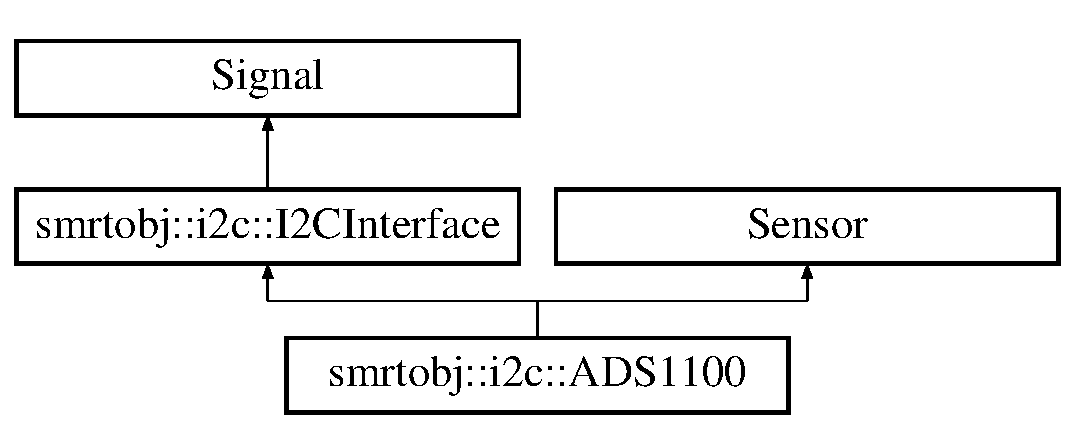
\includegraphics[height=3.000000cm]{classsmrtobj_1_1i2c_1_1_a_d_s1100}
\end{center}
\end{figure}
\subsection*{Public Member Functions}
\begin{DoxyCompactItemize}
\item 
\hyperlink{classsmrtobj_1_1i2c_1_1_a_d_s1100_a52f87f6cbfdc26c07a2c9bfa9e703928}{A\+D\+S1100} ()
\item 
\hyperlink{classsmrtobj_1_1i2c_1_1_a_d_s1100_a22e0bfc04d0cf6eb9c4a56e643b20a7e}{A\+D\+S1100} (uint8\+\_\+t addr)
\item 
\hyperlink{classsmrtobj_1_1i2c_1_1_a_d_s1100_a04610e29101e86c39e786c17b756e960}{A\+D\+S1100} (const \hyperlink{classsmrtobj_1_1i2c_1_1_a_d_s1100}{A\+D\+S1100} \&d)
\item 
virtual \hyperlink{classsmrtobj_1_1i2c_1_1_a_d_s1100_a658ca003cc76799a7199e1c38e34d1ea}{$\sim$\+A\+D\+S1100} ()
\item 
\hyperlink{classsmrtobj_1_1i2c_1_1_a_d_s1100}{A\+D\+S1100} \& \hyperlink{classsmrtobj_1_1i2c_1_1_a_d_s1100_ac023e56015781bc14ed0af5da16e4adb}{operator=} (const \hyperlink{classsmrtobj_1_1i2c_1_1_a_d_s1100}{A\+D\+S1100} \&d)
\item 
virtual bool \hyperlink{classsmrtobj_1_1i2c_1_1_a_d_s1100_af6a30ae17ea283aa979bbd933d84ee08}{initialize} ()
\item 
virtual bool \hyperlink{classsmrtobj_1_1i2c_1_1_a_d_s1100_a707ea27963bcca7465d51195cee0af04}{is\+Connected} ()
\item 
virtual bool \hyperlink{classsmrtobj_1_1i2c_1_1_a_d_s1100_ae57857e0b925c23af5406773bbaa3da9}{read} ()
\item 
virtual float \hyperlink{classsmrtobj_1_1i2c_1_1_a_d_s1100_ade27b68b0e321e5a8bd79fd119725f04}{measure} ()
\item 
uint16\+\_\+t \hyperlink{classsmrtobj_1_1i2c_1_1_a_d_s1100_aaf1867906432c5de522d7f3f0cd889c5}{value} ()
\end{DoxyCompactItemize}
\subsection*{Static Public Attributes}
\begin{DoxyCompactItemize}
\item 
\hypertarget{classsmrtobj_1_1i2c_1_1_a_d_s1100_afa5602c2717ec53e4401a1d31bb1d0dd}{}static const uint8\+\_\+t \hyperlink{classsmrtobj_1_1i2c_1_1_a_d_s1100_afa5602c2717ec53e4401a1d31bb1d0dd}{D\+E\+V\+I\+C\+E\+\_\+\+A\+D\+D\+R\+E\+S\+S} = 0x48\label{classsmrtobj_1_1i2c_1_1_a_d_s1100_afa5602c2717ec53e4401a1d31bb1d0dd}

\begin{DoxyCompactList}\small\item\em Device address used by default. \end{DoxyCompactList}\end{DoxyCompactItemize}
\subsection*{Additional Inherited Members}


\subsection{Detailed Description}
Class \hyperlink{classsmrtobj_1_1i2c_1_1_a_d_s1100}{A\+D\+S1100} models the Analog-\/to-\/\+Digital (A/\+D) converter T\+I \hyperlink{classsmrtobj_1_1i2c_1_1_a_d_s1100}{A\+D\+S1100}. The \hyperlink{classsmrtobj_1_1i2c_1_1_a_d_s1100}{A\+D\+S1100} is a precision, continuously self-\/calibrating A\+D\+C with differential inputs and up to 16 bits of resolution in a small S\+O\+T23-\/6 package. Conversions are performed ratiometrically, using the power supply as the reference voltage. The \hyperlink{classsmrtobj_1_1i2c_1_1_a_d_s1100}{A\+D\+S1100} uses an I2\+C-\/compatible serial interface and operates from a single power supply ranging from 2.\+7\+V to 5.\+5\+V. 

Definition at line 27 of file A\+D\+S1100.\+h.



\subsection{Constructor \& Destructor Documentation}
\hypertarget{classsmrtobj_1_1i2c_1_1_a_d_s1100_a52f87f6cbfdc26c07a2c9bfa9e703928}{}\index{smrtobj\+::i2c\+::\+A\+D\+S1100@{smrtobj\+::i2c\+::\+A\+D\+S1100}!A\+D\+S1100@{A\+D\+S1100}}
\index{A\+D\+S1100@{A\+D\+S1100}!smrtobj\+::i2c\+::\+A\+D\+S1100@{smrtobj\+::i2c\+::\+A\+D\+S1100}}
\subsubsection[{A\+D\+S1100()}]{\setlength{\rightskip}{0pt plus 5cm}smrtobj\+::i2c\+::\+A\+D\+S1100\+::\+A\+D\+S1100 (
\begin{DoxyParamCaption}
{}
\end{DoxyParamCaption}
)}\label{classsmrtobj_1_1i2c_1_1_a_d_s1100_a52f87f6cbfdc26c07a2c9bfa9e703928}
Default Constructor. 

Definition at line 16 of file A\+D\+S1100.\+cpp.

\hypertarget{classsmrtobj_1_1i2c_1_1_a_d_s1100_a22e0bfc04d0cf6eb9c4a56e643b20a7e}{}\index{smrtobj\+::i2c\+::\+A\+D\+S1100@{smrtobj\+::i2c\+::\+A\+D\+S1100}!A\+D\+S1100@{A\+D\+S1100}}
\index{A\+D\+S1100@{A\+D\+S1100}!smrtobj\+::i2c\+::\+A\+D\+S1100@{smrtobj\+::i2c\+::\+A\+D\+S1100}}
\subsubsection[{A\+D\+S1100(uint8\+\_\+t addr)}]{\setlength{\rightskip}{0pt plus 5cm}smrtobj\+::i2c\+::\+A\+D\+S1100\+::\+A\+D\+S1100 (
\begin{DoxyParamCaption}
\item[{uint8\+\_\+t}]{addr}
\end{DoxyParamCaption}
)}\label{classsmrtobj_1_1i2c_1_1_a_d_s1100_a22e0bfc04d0cf6eb9c4a56e643b20a7e}
Constructor. Sets the device address.


\begin{DoxyParams}[1]{Parameters}
\mbox{\tt in}  & {\em addr} & device address \\
\hline
\end{DoxyParams}


Definition at line 21 of file A\+D\+S1100.\+cpp.

\hypertarget{classsmrtobj_1_1i2c_1_1_a_d_s1100_a04610e29101e86c39e786c17b756e960}{}\index{smrtobj\+::i2c\+::\+A\+D\+S1100@{smrtobj\+::i2c\+::\+A\+D\+S1100}!A\+D\+S1100@{A\+D\+S1100}}
\index{A\+D\+S1100@{A\+D\+S1100}!smrtobj\+::i2c\+::\+A\+D\+S1100@{smrtobj\+::i2c\+::\+A\+D\+S1100}}
\subsubsection[{A\+D\+S1100(const A\+D\+S1100 \&d)}]{\setlength{\rightskip}{0pt plus 5cm}smrtobj\+::i2c\+::\+A\+D\+S1100\+::\+A\+D\+S1100 (
\begin{DoxyParamCaption}
\item[{const {\bf A\+D\+S1100} \&}]{d}
\end{DoxyParamCaption}
)}\label{classsmrtobj_1_1i2c_1_1_a_d_s1100_a04610e29101e86c39e786c17b756e960}
Copy Constructor.


\begin{DoxyParams}[1]{Parameters}
\mbox{\tt in}  & {\em d} & i2c device object \\
\hline
\end{DoxyParams}


Definition at line 26 of file A\+D\+S1100.\+cpp.

\hypertarget{classsmrtobj_1_1i2c_1_1_a_d_s1100_a658ca003cc76799a7199e1c38e34d1ea}{}\index{smrtobj\+::i2c\+::\+A\+D\+S1100@{smrtobj\+::i2c\+::\+A\+D\+S1100}!````~A\+D\+S1100@{$\sim$\+A\+D\+S1100}}
\index{````~A\+D\+S1100@{$\sim$\+A\+D\+S1100}!smrtobj\+::i2c\+::\+A\+D\+S1100@{smrtobj\+::i2c\+::\+A\+D\+S1100}}
\subsubsection[{$\sim$\+A\+D\+S1100()}]{\setlength{\rightskip}{0pt plus 5cm}smrtobj\+::i2c\+::\+A\+D\+S1100\+::$\sim$\+A\+D\+S1100 (
\begin{DoxyParamCaption}
{}
\end{DoxyParamCaption}
)\hspace{0.3cm}{\ttfamily [virtual]}}\label{classsmrtobj_1_1i2c_1_1_a_d_s1100_a658ca003cc76799a7199e1c38e34d1ea}
Destructor. 

Definition at line 31 of file A\+D\+S1100.\+cpp.



\subsection{Member Function Documentation}
\hypertarget{classsmrtobj_1_1i2c_1_1_a_d_s1100_af6a30ae17ea283aa979bbd933d84ee08}{}\index{smrtobj\+::i2c\+::\+A\+D\+S1100@{smrtobj\+::i2c\+::\+A\+D\+S1100}!initialize@{initialize}}
\index{initialize@{initialize}!smrtobj\+::i2c\+::\+A\+D\+S1100@{smrtobj\+::i2c\+::\+A\+D\+S1100}}
\subsubsection[{initialize()}]{\setlength{\rightskip}{0pt plus 5cm}bool smrtobj\+::i2c\+::\+A\+D\+S1100\+::initialize (
\begin{DoxyParamCaption}
{}
\end{DoxyParamCaption}
)\hspace{0.3cm}{\ttfamily [virtual]}}\label{classsmrtobj_1_1i2c_1_1_a_d_s1100_af6a30ae17ea283aa979bbd933d84ee08}
Initializes the i2c device\+: power on and prepare for general usage. Nothing is required by this device, it returns always true

\begin{DoxyReturn}{Returns}
always true. 
\end{DoxyReturn}


Implements \hyperlink{classsmrtobj_1_1i2c_1_1_i2_c_interface_a4ff1ff083d877c7c0816299b11965eb4}{smrtobj\+::i2c\+::\+I2\+C\+Interface}.



Definition at line 46 of file A\+D\+S1100.\+cpp.

\hypertarget{classsmrtobj_1_1i2c_1_1_a_d_s1100_a707ea27963bcca7465d51195cee0af04}{}\index{smrtobj\+::i2c\+::\+A\+D\+S1100@{smrtobj\+::i2c\+::\+A\+D\+S1100}!is\+Connected@{is\+Connected}}
\index{is\+Connected@{is\+Connected}!smrtobj\+::i2c\+::\+A\+D\+S1100@{smrtobj\+::i2c\+::\+A\+D\+S1100}}
\subsubsection[{is\+Connected()}]{\setlength{\rightskip}{0pt plus 5cm}bool smrtobj\+::i2c\+::\+A\+D\+S1100\+::is\+Connected (
\begin{DoxyParamCaption}
{}
\end{DoxyParamCaption}
)\hspace{0.3cm}{\ttfamily [virtual]}}\label{classsmrtobj_1_1i2c_1_1_a_d_s1100_a707ea27963bcca7465d51195cee0af04}
Tests if the device is connected. Make sure the device is connected and responds as expected.

\begin{DoxyReturn}{Returns}
true if connection is valid, false otherwise 
\end{DoxyReturn}


Implements \hyperlink{classsmrtobj_1_1i2c_1_1_i2_c_interface_a33fd37bafaf8c7e8184acb6470322bce}{smrtobj\+::i2c\+::\+I2\+C\+Interface}.



Definition at line 52 of file A\+D\+S1100.\+cpp.

\hypertarget{classsmrtobj_1_1i2c_1_1_a_d_s1100_ade27b68b0e321e5a8bd79fd119725f04}{}\index{smrtobj\+::i2c\+::\+A\+D\+S1100@{smrtobj\+::i2c\+::\+A\+D\+S1100}!measure@{measure}}
\index{measure@{measure}!smrtobj\+::i2c\+::\+A\+D\+S1100@{smrtobj\+::i2c\+::\+A\+D\+S1100}}
\subsubsection[{measure()}]{\setlength{\rightskip}{0pt plus 5cm}float smrtobj\+::i2c\+::\+A\+D\+S1100\+::measure (
\begin{DoxyParamCaption}
{}
\end{DoxyParamCaption}
)\hspace{0.3cm}{\ttfamily [virtual]}}\label{classsmrtobj_1_1i2c_1_1_a_d_s1100_ade27b68b0e321e5a8bd79fd119725f04}
Converts data read (saved in {\itshape m\+\_\+value} variable) in voltage. Note\+: To be changed!! now it use the formula of A\+D\+S1110. Example\+:


\begin{DoxyCode}
smrtobj::i2c::ASD1100 adc(0x48);

\textcolor{comment}{// Test if device is connected }
\textcolor{keywordflow}{if}( adc.isConnected() )
\{
  \textcolor{keywordflow}{if} ( adc.read() )
  \{
    \textcolor{keywordtype}{float} voltage = adc.measure();
    ...
  \}
\}
\end{DoxyCode}


\begin{DoxyReturn}{Returns}
last data read as voltage level. 
\end{DoxyReturn}


Definition at line 67 of file A\+D\+S1100.\+cpp.

\hypertarget{classsmrtobj_1_1i2c_1_1_a_d_s1100_ac023e56015781bc14ed0af5da16e4adb}{}\index{smrtobj\+::i2c\+::\+A\+D\+S1100@{smrtobj\+::i2c\+::\+A\+D\+S1100}!operator=@{operator=}}
\index{operator=@{operator=}!smrtobj\+::i2c\+::\+A\+D\+S1100@{smrtobj\+::i2c\+::\+A\+D\+S1100}}
\subsubsection[{operator=(const A\+D\+S1100 \&d)}]{\setlength{\rightskip}{0pt plus 5cm}{\bf A\+D\+S1100} \& smrtobj\+::i2c\+::\+A\+D\+S1100\+::operator= (
\begin{DoxyParamCaption}
\item[{const {\bf A\+D\+S1100} \&}]{d}
\end{DoxyParamCaption}
)}\label{classsmrtobj_1_1i2c_1_1_a_d_s1100_ac023e56015781bc14ed0af5da16e4adb}
Override operator =


\begin{DoxyParams}[1]{Parameters}
\mbox{\tt in}  & {\em d} & source device object\\
\hline
\end{DoxyParams}
\begin{DoxyReturn}{Returns}
destination device reference 
\end{DoxyReturn}


Definition at line 35 of file A\+D\+S1100.\+cpp.

\hypertarget{classsmrtobj_1_1i2c_1_1_a_d_s1100_ae57857e0b925c23af5406773bbaa3da9}{}\index{smrtobj\+::i2c\+::\+A\+D\+S1100@{smrtobj\+::i2c\+::\+A\+D\+S1100}!read@{read}}
\index{read@{read}!smrtobj\+::i2c\+::\+A\+D\+S1100@{smrtobj\+::i2c\+::\+A\+D\+S1100}}
\subsubsection[{read()}]{\setlength{\rightskip}{0pt plus 5cm}bool smrtobj\+::i2c\+::\+A\+D\+S1100\+::read (
\begin{DoxyParamCaption}
{}
\end{DoxyParamCaption}
)\hspace{0.3cm}{\ttfamily [virtual]}}\label{classsmrtobj_1_1i2c_1_1_a_d_s1100_ae57857e0b925c23af5406773bbaa3da9}
Reads data from the i2c device. This function read 2 byte\+:
\begin{DoxyItemize}
\item 1st byte (Byte0) is the most significant byte
\item 2nd byte (Byte1) is the less significant byte
\end{DoxyItemize}

Data is calculate as\+:


\begin{DoxyCode}
\hyperlink{classsmrtobj_1_1i2c_1_1_a_d_s1100_aaf1867906432c5de522d7f3f0cd889c5}{value} = (Byte0] << 8) | Byte1;
\end{DoxyCode}


The value read is stored in the internal buffer ({\itshape m\+\_\+value}).

\begin{DoxyReturn}{Returns}
true for success, or false if any error occurs. 
\end{DoxyReturn}


Implements \hyperlink{classsmrtobj_1_1i2c_1_1_i2_c_interface_a58bc734662a60de6a7cb7976c2179753}{smrtobj\+::i2c\+::\+I2\+C\+Interface}.



Definition at line 62 of file A\+D\+S1100.\+cpp.

\hypertarget{classsmrtobj_1_1i2c_1_1_a_d_s1100_aaf1867906432c5de522d7f3f0cd889c5}{}\index{smrtobj\+::i2c\+::\+A\+D\+S1100@{smrtobj\+::i2c\+::\+A\+D\+S1100}!value@{value}}
\index{value@{value}!smrtobj\+::i2c\+::\+A\+D\+S1100@{smrtobj\+::i2c\+::\+A\+D\+S1100}}
\subsubsection[{value()}]{\setlength{\rightskip}{0pt plus 5cm}uint16\+\_\+t smrtobj\+::i2c\+::\+A\+D\+S1100\+::value (
\begin{DoxyParamCaption}
{}
\end{DoxyParamCaption}
)\hspace{0.3cm}{\ttfamily [inline]}}\label{classsmrtobj_1_1i2c_1_1_a_d_s1100_aaf1867906432c5de522d7f3f0cd889c5}
Returns last A\+D\+C value read. Example\+:


\begin{DoxyCode}
smrtobj::i2c::ASD1100 adc(0x48);

\textcolor{comment}{// Test if device is connected }
\textcolor{keywordflow}{if}( adc.isConnected() )
\{
  \textcolor{keywordflow}{if} ( adc.read() )
  \{
    uint16\_t adc\_value = adc.value();
    ...
  \}
\}
\end{DoxyCode}


\begin{DoxyReturn}{Returns}
last value read 
\end{DoxyReturn}


Definition at line 142 of file A\+D\+S1100.\+h.



The documentation for this class was generated from the following files\+:\begin{DoxyCompactItemize}
\item 
libraries/\+Smrt\+Obj\+I2\+C/src/sensors/\hyperlink{_a_d_s1100_8h}{A\+D\+S1100.\+h}\item 
libraries/\+Smrt\+Obj\+I2\+C/src/sensors/\hyperlink{_a_d_s1100_8cpp}{A\+D\+S1100.\+cpp}\end{DoxyCompactItemize}

\hypertarget{classsmrtobj_1_1io_1_1_analog_input}{}\section{smrtobj\+:\+:io\+:\+:Analog\+Input Class Reference}
\label{classsmrtobj_1_1io_1_1_analog_input}\index{smrtobj\+::io\+::\+Analog\+Input@{smrtobj\+::io\+::\+Analog\+Input}}


{\ttfamily \#include $<$iosignal.\+h$>$}

Inheritance diagram for smrtobj\+:\+:io\+:\+:Analog\+Input\+:\begin{figure}[H]
\begin{center}
\leavevmode
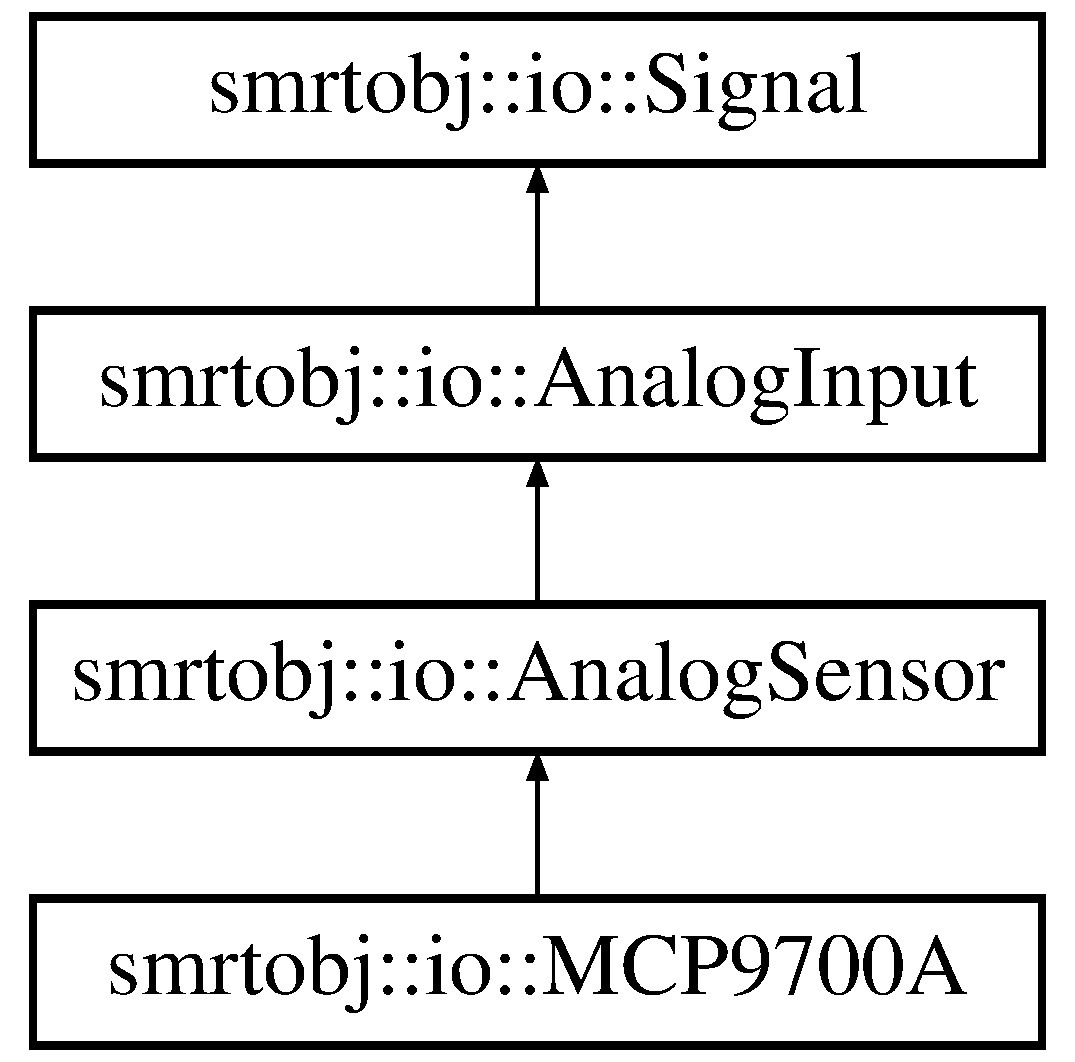
\includegraphics[height=4.000000cm]{classsmrtobj_1_1io_1_1_analog_input}
\end{center}
\end{figure}
\subsection*{Public Types}
\begin{DoxyCompactItemize}
\item 
enum \hyperlink{classsmrtobj_1_1io_1_1_analog_input_a4e2bf85b374d5856fc0dee0225fbd025}{\+\_\+v\+\_\+default} \{ \hyperlink{classsmrtobj_1_1io_1_1_analog_input_a4e2bf85b374d5856fc0dee0225fbd025a61b0cbe28d17a05cb3a268398c370cb9}{V0\+\_\+0} = 0, 
\hyperlink{classsmrtobj_1_1io_1_1_analog_input_a4e2bf85b374d5856fc0dee0225fbd025a2692641238f0ae5eb558d1f9c1688604}{V5\+\_\+0} = 1, 
\hyperlink{classsmrtobj_1_1io_1_1_analog_input_a4e2bf85b374d5856fc0dee0225fbd025aac4c61fd6d37aacbf3bd6a3be6d835d3}{V3\+\_\+3} = 2
 \}
\end{DoxyCompactItemize}
\subsection*{Public Member Functions}
\begin{DoxyCompactItemize}
\item 
\hyperlink{classsmrtobj_1_1io_1_1_analog_input_a40008473025615c63d22cf82091f1c49}{Analog\+Input} ()
\item 
\hyperlink{classsmrtobj_1_1io_1_1_analog_input_a3cf704d9977129fc9548f4d10d344dcc}{Analog\+Input} (const \hyperlink{classsmrtobj_1_1io_1_1_analog_input}{Analog\+Input} \&o)
\item 
virtual \hyperlink{classsmrtobj_1_1io_1_1_analog_input_a663423c6a8c4556498b8b7c15ad2f163}{$\sim$\+Analog\+Input} ()
\item 
\hyperlink{classsmrtobj_1_1io_1_1_analog_input}{Analog\+Input} \& \hyperlink{classsmrtobj_1_1io_1_1_analog_input_a98027675f727183bc289d5276eb1f38e}{operator=} (const \hyperlink{classsmrtobj_1_1io_1_1_analog_input}{Analog\+Input} \&i)
\item 
byte \hyperlink{classsmrtobj_1_1io_1_1_analog_input_a08fe1be7aca445768e1b2293cb48b96a}{type} ()
\item 
void \hyperlink{classsmrtobj_1_1io_1_1_analog_input_a05e6a75658d9c5d9c5b9cbfffb8e2a91}{init} (byte \hyperlink{classsmrtobj_1_1io_1_1_analog_input_a5768f6b56a7ad5b9eb7da2b95951d5e6}{pin}, bool pullup=false)
\item 
unsigned long \hyperlink{classsmrtobj_1_1io_1_1_analog_input_aa223ad3c6350b5f94f8563870134f4e3}{value} ()
\item 
byte \hyperlink{classsmrtobj_1_1io_1_1_analog_input_a5768f6b56a7ad5b9eb7da2b95951d5e6}{pin} ()
\item 
unsigned long \hyperlink{classsmrtobj_1_1io_1_1_analog_input_aed112dc7b72d12075c93a5ca29a661f7}{read} ()
\item 
float \hyperlink{classsmrtobj_1_1io_1_1_analog_input_a99054ad9e24ffa6d1f2d5832ff3ad640}{input\+Voltage} ()
\end{DoxyCompactItemize}
\subsection*{Static Public Member Functions}
\begin{DoxyCompactItemize}
\item 
static float \hyperlink{classsmrtobj_1_1io_1_1_analog_input_a71d194e2abf9852b8ac5d0750568be4c}{reference} ()
\item 
static bool \hyperlink{classsmrtobj_1_1io_1_1_analog_input_aec6587007c8d16a2483e22fbf621631e}{set\+Reference\+Default} (byte vdef=\hyperlink{classsmrtobj_1_1io_1_1_analog_input_a4e2bf85b374d5856fc0dee0225fbd025a2692641238f0ae5eb558d1f9c1688604}{V5\+\_\+0})
\item 
static bool \hyperlink{classsmrtobj_1_1io_1_1_analog_input_a868ba4197c49394a0e0c70bd47ca2074}{set\+Reference} (float voltage)
\end{DoxyCompactItemize}
\subsection*{Static Public Attributes}
\begin{DoxyCompactItemize}
\item 
\hypertarget{classsmrtobj_1_1io_1_1_analog_input_af12741094c2f05dfdb9598bac6c78e6c}{}static const byte \hyperlink{classsmrtobj_1_1io_1_1_analog_input_af12741094c2f05dfdb9598bac6c78e6c}{R\+E\+S\+O\+L\+U\+T\+I\+O\+N} = 10\label{classsmrtobj_1_1io_1_1_analog_input_af12741094c2f05dfdb9598bac6c78e6c}

\begin{DoxyCompactList}\small\item\em A\+D\+C resolution. \end{DoxyCompactList}\item 
\hypertarget{classsmrtobj_1_1io_1_1_analog_input_a170725a849e4b1676d739c7c7b96ee71}{}static const float \hyperlink{classsmrtobj_1_1io_1_1_analog_input_a170725a849e4b1676d739c7c7b96ee71}{D\+E\+F\+A\+U\+L\+T\+\_\+\+V\+R\+E\+F} = 5.\+0\label{classsmrtobj_1_1io_1_1_analog_input_a170725a849e4b1676d739c7c7b96ee71}

\begin{DoxyCompactList}\small\item\em Default A\+D\+C reference voltage. \end{DoxyCompactList}\end{DoxyCompactItemize}
\subsection*{Additional Inherited Members}


\subsection{Detailed Description}
The \hyperlink{classsmrtobj_1_1io_1_1_analog_input}{Analog\+Input} class models a analog input. Using this, it is possible read the value from a specified analog pin.

The Arduino board contains a 6 channel (8 channels on the Mini and Nano, 16 on the Mega), 10-\/bit analog to digital converter. This means that it will map input voltages between 0 and 5 volts into integer values between 0 and 1023. This yields a resolution between readings of\+: 5 volts / 1024 units or, .0049 volts (4.\+9 m\+V) per unit. The input range and resolution can be changed using analog\+Reference().

It takes about 100 microseconds (0.\+0001 s) to read an analog input, so the maximum reading rate is about 10,000 times a second. 

Definition at line 303 of file iosignal.\+h.



\subsection{Member Enumeration Documentation}
\hypertarget{classsmrtobj_1_1io_1_1_analog_input_a4e2bf85b374d5856fc0dee0225fbd025}{}\index{smrtobj\+::io\+::\+Analog\+Input@{smrtobj\+::io\+::\+Analog\+Input}!\+\_\+v\+\_\+default@{\+\_\+v\+\_\+default}}
\index{\+\_\+v\+\_\+default@{\+\_\+v\+\_\+default}!smrtobj\+::io\+::\+Analog\+Input@{smrtobj\+::io\+::\+Analog\+Input}}
\subsubsection[{\+\_\+v\+\_\+default}]{\setlength{\rightskip}{0pt plus 5cm}enum {\bf smrtobj\+::io\+::\+Analog\+Input\+::\+\_\+v\+\_\+default}}\label{classsmrtobj_1_1io_1_1_analog_input_a4e2bf85b374d5856fc0dee0225fbd025}
Default reference voltage \begin{Desc}
\item[Enumerator]\par
\begin{description}
\index{V0\+\_\+0@{V0\+\_\+0}!smrtobj\+::io\+::\+Analog\+Input@{smrtobj\+::io\+::\+Analog\+Input}}\index{smrtobj\+::io\+::\+Analog\+Input@{smrtobj\+::io\+::\+Analog\+Input}!V0\+\_\+0@{V0\+\_\+0}}\item[{\em 
\hypertarget{classsmrtobj_1_1io_1_1_analog_input_a4e2bf85b374d5856fc0dee0225fbd025a61b0cbe28d17a05cb3a268398c370cb9}{}V0\+\_\+0\label{classsmrtobj_1_1io_1_1_analog_input_a4e2bf85b374d5856fc0dee0225fbd025a61b0cbe28d17a05cb3a268398c370cb9}
}]Off, 0.\+0 Volt. \index{V5\+\_\+0@{V5\+\_\+0}!smrtobj\+::io\+::\+Analog\+Input@{smrtobj\+::io\+::\+Analog\+Input}}\index{smrtobj\+::io\+::\+Analog\+Input@{smrtobj\+::io\+::\+Analog\+Input}!V5\+\_\+0@{V5\+\_\+0}}\item[{\em 
\hypertarget{classsmrtobj_1_1io_1_1_analog_input_a4e2bf85b374d5856fc0dee0225fbd025a2692641238f0ae5eb558d1f9c1688604}{}V5\+\_\+0\label{classsmrtobj_1_1io_1_1_analog_input_a4e2bf85b374d5856fc0dee0225fbd025a2692641238f0ae5eb558d1f9c1688604}
}]5.\+0 Volt \index{V3\+\_\+3@{V3\+\_\+3}!smrtobj\+::io\+::\+Analog\+Input@{smrtobj\+::io\+::\+Analog\+Input}}\index{smrtobj\+::io\+::\+Analog\+Input@{smrtobj\+::io\+::\+Analog\+Input}!V3\+\_\+3@{V3\+\_\+3}}\item[{\em 
\hypertarget{classsmrtobj_1_1io_1_1_analog_input_a4e2bf85b374d5856fc0dee0225fbd025aac4c61fd6d37aacbf3bd6a3be6d835d3}{}V3\+\_\+3\label{classsmrtobj_1_1io_1_1_analog_input_a4e2bf85b374d5856fc0dee0225fbd025aac4c61fd6d37aacbf3bd6a3be6d835d3}
}]3.\+3 Volt \end{description}
\end{Desc}


Definition at line 315 of file iosignal.\+h.



\subsection{Constructor \& Destructor Documentation}
\hypertarget{classsmrtobj_1_1io_1_1_analog_input_a40008473025615c63d22cf82091f1c49}{}\index{smrtobj\+::io\+::\+Analog\+Input@{smrtobj\+::io\+::\+Analog\+Input}!Analog\+Input@{Analog\+Input}}
\index{Analog\+Input@{Analog\+Input}!smrtobj\+::io\+::\+Analog\+Input@{smrtobj\+::io\+::\+Analog\+Input}}
\subsubsection[{Analog\+Input()}]{\setlength{\rightskip}{0pt plus 5cm}smrtobj\+::io\+::\+Analog\+Input\+::\+Analog\+Input (
\begin{DoxyParamCaption}
{}
\end{DoxyParamCaption}
)}\label{classsmrtobj_1_1io_1_1_analog_input_a40008473025615c63d22cf82091f1c49}
Default Constructor It initializes the last value read to 0 and the pin number to 0. 

Definition at line 208 of file iosignal.\+cpp.

\hypertarget{classsmrtobj_1_1io_1_1_analog_input_a3cf704d9977129fc9548f4d10d344dcc}{}\index{smrtobj\+::io\+::\+Analog\+Input@{smrtobj\+::io\+::\+Analog\+Input}!Analog\+Input@{Analog\+Input}}
\index{Analog\+Input@{Analog\+Input}!smrtobj\+::io\+::\+Analog\+Input@{smrtobj\+::io\+::\+Analog\+Input}}
\subsubsection[{Analog\+Input(const Analog\+Input \&o)}]{\setlength{\rightskip}{0pt plus 5cm}smrtobj\+::io\+::\+Analog\+Input\+::\+Analog\+Input (
\begin{DoxyParamCaption}
\item[{const {\bf Analog\+Input} \&}]{o}
\end{DoxyParamCaption}
)}\label{classsmrtobj_1_1io_1_1_analog_input_a3cf704d9977129fc9548f4d10d344dcc}
Copy Constructor


\begin{DoxyParams}[1]{Parameters}
\mbox{\tt in}  & {\em o} & source digital input\\
\hline
\end{DoxyParams}
\begin{DoxyReturn}{Returns}
reference to the destination digital input object 
\end{DoxyReturn}


Definition at line 213 of file iosignal.\+cpp.

\hypertarget{classsmrtobj_1_1io_1_1_analog_input_a663423c6a8c4556498b8b7c15ad2f163}{}\index{smrtobj\+::io\+::\+Analog\+Input@{smrtobj\+::io\+::\+Analog\+Input}!````~Analog\+Input@{$\sim$\+Analog\+Input}}
\index{````~Analog\+Input@{$\sim$\+Analog\+Input}!smrtobj\+::io\+::\+Analog\+Input@{smrtobj\+::io\+::\+Analog\+Input}}
\subsubsection[{$\sim$\+Analog\+Input()}]{\setlength{\rightskip}{0pt plus 5cm}smrtobj\+::io\+::\+Analog\+Input\+::$\sim$\+Analog\+Input (
\begin{DoxyParamCaption}
{}
\end{DoxyParamCaption}
)\hspace{0.3cm}{\ttfamily [virtual]}}\label{classsmrtobj_1_1io_1_1_analog_input_a663423c6a8c4556498b8b7c15ad2f163}
Destructor 

Definition at line 219 of file iosignal.\+cpp.



\subsection{Member Function Documentation}
\hypertarget{classsmrtobj_1_1io_1_1_analog_input_a05e6a75658d9c5d9c5b9cbfffb8e2a91}{}\index{smrtobj\+::io\+::\+Analog\+Input@{smrtobj\+::io\+::\+Analog\+Input}!init@{init}}
\index{init@{init}!smrtobj\+::io\+::\+Analog\+Input@{smrtobj\+::io\+::\+Analog\+Input}}
\subsubsection[{init(byte pin, bool pullup=false)}]{\setlength{\rightskip}{0pt plus 5cm}void smrtobj\+::io\+::\+Analog\+Input\+::init (
\begin{DoxyParamCaption}
\item[{byte}]{pin, }
\item[{bool}]{pullup = {\ttfamily false}}
\end{DoxyParamCaption}
)}\label{classsmrtobj_1_1io_1_1_analog_input_a05e6a75658d9c5d9c5b9cbfffb8e2a91}
Opens the pin in input mode. It is possible use internal pull up resistor.~\newline
The analog pins also have pullup resistors, which work identically to pullup resistors on the digital pins.~\newline
Be aware however that turning on a pullup will affect the values reported by analog\+Read().


\begin{DoxyParams}[1]{Parameters}
\mbox{\tt in}  & {\em pin} & number of the input pin \\
\hline
\mbox{\tt in}  & {\em pullup} & use internal pull up resistor. Default value is false \\
\hline
\end{DoxyParams}


Definition at line 232 of file iosignal.\+cpp.

\hypertarget{classsmrtobj_1_1io_1_1_analog_input_a99054ad9e24ffa6d1f2d5832ff3ad640}{}\index{smrtobj\+::io\+::\+Analog\+Input@{smrtobj\+::io\+::\+Analog\+Input}!input\+Voltage@{input\+Voltage}}
\index{input\+Voltage@{input\+Voltage}!smrtobj\+::io\+::\+Analog\+Input@{smrtobj\+::io\+::\+Analog\+Input}}
\subsubsection[{input\+Voltage()}]{\setlength{\rightskip}{0pt plus 5cm}float smrtobj\+::io\+::\+Analog\+Input\+::input\+Voltage (
\begin{DoxyParamCaption}
{}
\end{DoxyParamCaption}
)}\label{classsmrtobj_1_1io_1_1_analog_input_a99054ad9e24ffa6d1f2d5832ff3ad640}
Gets value as voltage. Pay attention, this value depends on reference voltage, if it has been set a wrong value for this voltage, function will return a wrong result. See \#smrtobj\+::\+Analog\+Sensor\+::set\+Reference\+Default and \hyperlink{classsmrtobj_1_1io_1_1_analog_input_a868ba4197c49394a0e0c70bd47ca2074}{smrtobj\+::io\+::\+Analog\+Sensor\+::set\+Reference}

\begin{DoxyReturn}{Returns}
input value as voltage 
\end{DoxyReturn}


Definition at line 256 of file iosignal.\+cpp.

\hypertarget{classsmrtobj_1_1io_1_1_analog_input_a98027675f727183bc289d5276eb1f38e}{}\index{smrtobj\+::io\+::\+Analog\+Input@{smrtobj\+::io\+::\+Analog\+Input}!operator=@{operator=}}
\index{operator=@{operator=}!smrtobj\+::io\+::\+Analog\+Input@{smrtobj\+::io\+::\+Analog\+Input}}
\subsubsection[{operator=(const Analog\+Input \&i)}]{\setlength{\rightskip}{0pt plus 5cm}{\bf Analog\+Input} \& smrtobj\+::io\+::\+Analog\+Input\+::operator= (
\begin{DoxyParamCaption}
\item[{const {\bf Analog\+Input} \&}]{i}
\end{DoxyParamCaption}
)}\label{classsmrtobj_1_1io_1_1_analog_input_a98027675f727183bc289d5276eb1f38e}
Override operator = 

Definition at line 223 of file iosignal.\+cpp.

\hypertarget{classsmrtobj_1_1io_1_1_analog_input_a5768f6b56a7ad5b9eb7da2b95951d5e6}{}\index{smrtobj\+::io\+::\+Analog\+Input@{smrtobj\+::io\+::\+Analog\+Input}!pin@{pin}}
\index{pin@{pin}!smrtobj\+::io\+::\+Analog\+Input@{smrtobj\+::io\+::\+Analog\+Input}}
\subsubsection[{pin()}]{\setlength{\rightskip}{0pt plus 5cm}byte smrtobj\+::io\+::\+Analog\+Input\+::pin (
\begin{DoxyParamCaption}
{}
\end{DoxyParamCaption}
)\hspace{0.3cm}{\ttfamily [inline]}}\label{classsmrtobj_1_1io_1_1_analog_input_a5768f6b56a7ad5b9eb7da2b95951d5e6}
Gets the number of the analog input pin.

\begin{DoxyReturn}{Returns}
pin number 
\end{DoxyReturn}


Definition at line 424 of file iosignal.\+h.

\hypertarget{classsmrtobj_1_1io_1_1_analog_input_aed112dc7b72d12075c93a5ca29a661f7}{}\index{smrtobj\+::io\+::\+Analog\+Input@{smrtobj\+::io\+::\+Analog\+Input}!read@{read}}
\index{read@{read}!smrtobj\+::io\+::\+Analog\+Input@{smrtobj\+::io\+::\+Analog\+Input}}
\subsubsection[{read()}]{\setlength{\rightskip}{0pt plus 5cm}unsigned long smrtobj\+::io\+::\+Analog\+Input\+::read (
\begin{DoxyParamCaption}
{}
\end{DoxyParamCaption}
)}\label{classsmrtobj_1_1io_1_1_analog_input_aed112dc7b72d12075c93a5ca29a661f7}
Reads value from the analog input. If the input has not been opened yet, it returns 0.

\begin{DoxyReturn}{Returns}
value, it is a number between 0 and 1023 
\end{DoxyReturn}


Definition at line 244 of file iosignal.\+cpp.

\hypertarget{classsmrtobj_1_1io_1_1_analog_input_a71d194e2abf9852b8ac5d0750568be4c}{}\index{smrtobj\+::io\+::\+Analog\+Input@{smrtobj\+::io\+::\+Analog\+Input}!reference@{reference}}
\index{reference@{reference}!smrtobj\+::io\+::\+Analog\+Input@{smrtobj\+::io\+::\+Analog\+Input}}
\subsubsection[{reference()}]{\setlength{\rightskip}{0pt plus 5cm}float smrtobj\+::io\+::\+Analog\+Input\+::reference (
\begin{DoxyParamCaption}
{}
\end{DoxyParamCaption}
)\hspace{0.3cm}{\ttfamily [static]}}\label{classsmrtobj_1_1io_1_1_analog_input_a71d194e2abf9852b8ac5d0750568be4c}
Gets reference voltage for A\+D\+Cs in volts

\begin{DoxyReturn}{Returns}
reference voltage for A\+D\+Cs 
\end{DoxyReturn}


Definition at line 175 of file iosignal.\+cpp.

\hypertarget{classsmrtobj_1_1io_1_1_analog_input_a868ba4197c49394a0e0c70bd47ca2074}{}\index{smrtobj\+::io\+::\+Analog\+Input@{smrtobj\+::io\+::\+Analog\+Input}!set\+Reference@{set\+Reference}}
\index{set\+Reference@{set\+Reference}!smrtobj\+::io\+::\+Analog\+Input@{smrtobj\+::io\+::\+Analog\+Input}}
\subsubsection[{set\+Reference(float voltage)}]{\setlength{\rightskip}{0pt plus 5cm}bool smrtobj\+::io\+::\+Analog\+Input\+::set\+Reference (
\begin{DoxyParamCaption}
\item[{float}]{voltage}
\end{DoxyParamCaption}
)\hspace{0.3cm}{\ttfamily [static]}}\label{classsmrtobj_1_1io_1_1_analog_input_a868ba4197c49394a0e0c70bd47ca2074}
Change reference for A\+D\+Cs, using external reference. The voltage applied to the A\+R\+E\+F pin (0 to 5\+V only) is used as the reference. It is suggested to initialize before the default voltage using smrtobj\+::\+Analog\+Sensor\+::set\+Reference\+Default before set an external reference voltage. If you use an invalid voltage as parameter, it will be use the default voltage and return false.

{\bfseries Note\+:} Check the correct default voltage for your Arduino board! This function sets this value in an internal attribute. If it is different from the actual board, reading will give a wrong result.


\begin{DoxyParams}[1]{Parameters}
\mbox{\tt in}  & {\em voltage} & the voltage applied to the A\+R\+E\+F pin (0 to 5\+V only).\\
\hline
\end{DoxyParams}
\begin{DoxyReturn}{Returns}
true if voltage is valid, false otherwise 
\end{DoxyReturn}


Definition at line 196 of file iosignal.\+cpp.

\hypertarget{classsmrtobj_1_1io_1_1_analog_input_aec6587007c8d16a2483e22fbf621631e}{}\index{smrtobj\+::io\+::\+Analog\+Input@{smrtobj\+::io\+::\+Analog\+Input}!set\+Reference\+Default@{set\+Reference\+Default}}
\index{set\+Reference\+Default@{set\+Reference\+Default}!smrtobj\+::io\+::\+Analog\+Input@{smrtobj\+::io\+::\+Analog\+Input}}
\subsubsection[{set\+Reference\+Default(byte vdef=\+V5\+\_\+0)}]{\setlength{\rightskip}{0pt plus 5cm}bool smrtobj\+::io\+::\+Analog\+Input\+::set\+Reference\+Default (
\begin{DoxyParamCaption}
\item[{byte}]{vdef = {\ttfamily {\bf V5\+\_\+0}}}
\end{DoxyParamCaption}
)\hspace{0.3cm}{\ttfamily [static]}}\label{classsmrtobj_1_1io_1_1_analog_input_aec6587007c8d16a2483e22fbf621631e}
Change reference for A\+D\+Cs, using default board value. Please check the working voltage for your Arduino board\+: default analog reference of 5 volts (on 5\+V Arduino boards) or 3.\+3 volts (on 3.\+3\+V Arduino boards). If {\ttfamily vdef} parameter is not valid (\#smrtobj\+::\+Analog\+Sensor\+::\+\_\+v\+\_\+default) all A\+D\+Cs will be turned off, putting the reference voltage to 0.\+0\+V.

{\bfseries Note\+:} Check the correct default voltage for your Arduino board! This function sets this value in an internal attribute. If it is different from the actual board, reading will give a wrong result.


\begin{DoxyParams}[1]{Parameters}
\mbox{\tt in}  & {\em vdef} & analog reference for your Arduino board according to \#smrtobj\+::\+Analog\+Sensor\+::\+\_\+v\+\_\+default enum.\\
\hline
\end{DoxyParams}
\begin{DoxyReturn}{Returns}
true if default voltage is correct, false otherwise 
\end{DoxyReturn}


Definition at line 180 of file iosignal.\+cpp.

\hypertarget{classsmrtobj_1_1io_1_1_analog_input_a08fe1be7aca445768e1b2293cb48b96a}{}\index{smrtobj\+::io\+::\+Analog\+Input@{smrtobj\+::io\+::\+Analog\+Input}!type@{type}}
\index{type@{type}!smrtobj\+::io\+::\+Analog\+Input@{smrtobj\+::io\+::\+Analog\+Input}}
\subsubsection[{type()}]{\setlength{\rightskip}{0pt plus 5cm}byte smrtobj\+::io\+::\+Analog\+Input\+::type (
\begin{DoxyParamCaption}
{}
\end{DoxyParamCaption}
)\hspace{0.3cm}{\ttfamily [inline]}, {\ttfamily [virtual]}}\label{classsmrtobj_1_1io_1_1_analog_input_a08fe1be7aca445768e1b2293cb48b96a}
Gets the type of the interface according to \#smrtobj\+::\+Signal\+::\+\_\+type enum

\begin{DoxyReturn}{Returns}
type of the interface 
\end{DoxyReturn}


Implements \hyperlink{classsmrtobj_1_1io_1_1_signal_a38cd36f413f1ad2213684e4364ac4270}{smrtobj\+::io\+::\+Signal}.



Definition at line 399 of file iosignal.\+h.

\hypertarget{classsmrtobj_1_1io_1_1_analog_input_aa223ad3c6350b5f94f8563870134f4e3}{}\index{smrtobj\+::io\+::\+Analog\+Input@{smrtobj\+::io\+::\+Analog\+Input}!value@{value}}
\index{value@{value}!smrtobj\+::io\+::\+Analog\+Input@{smrtobj\+::io\+::\+Analog\+Input}}
\subsubsection[{value()}]{\setlength{\rightskip}{0pt plus 5cm}unsigned long smrtobj\+::io\+::\+Analog\+Input\+::value (
\begin{DoxyParamCaption}
{}
\end{DoxyParamCaption}
)\hspace{0.3cm}{\ttfamily [inline]}}\label{classsmrtobj_1_1io_1_1_analog_input_aa223ad3c6350b5f94f8563870134f4e3}
Gets the last value read. If the input has not been opened yet, it returns 0.

\begin{DoxyReturn}{Returns}
last value read 
\end{DoxyReturn}


Definition at line 417 of file iosignal.\+h.



The documentation for this class was generated from the following files\+:\begin{DoxyCompactItemize}
\item 
libraries/\+Smrt\+Obj\+I\+O/src/\hyperlink{iosignal_8h}{iosignal.\+h}\item 
libraries/\+Smrt\+Obj\+I\+O/src/\hyperlink{iosignal_8cpp}{iosignal.\+cpp}\end{DoxyCompactItemize}

\hypertarget{classsmrtobj_1_1io_1_1_analog_sensor}{}\section{smrtobj\+:\+:io\+:\+:Analog\+Sensor Class Reference}
\label{classsmrtobj_1_1io_1_1_analog_sensor}\index{smrtobj\+::io\+::\+Analog\+Sensor@{smrtobj\+::io\+::\+Analog\+Sensor}}


{\ttfamily \#include $<$analogsensor.\+h$>$}

Inheritance diagram for smrtobj\+:\+:io\+:\+:Analog\+Sensor\+:\begin{figure}[H]
\begin{center}
\leavevmode
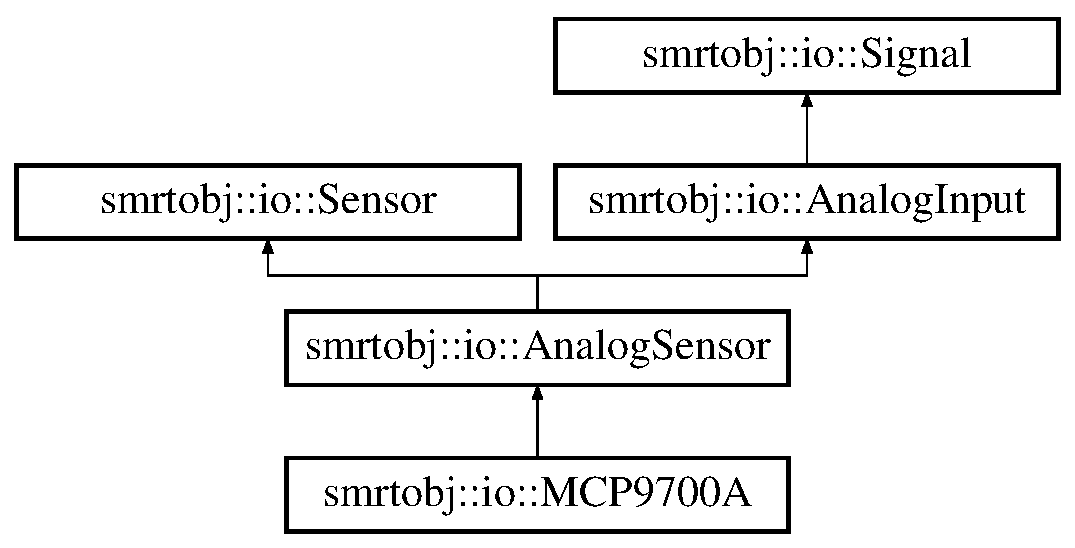
\includegraphics[height=4.000000cm]{classsmrtobj_1_1io_1_1_analog_sensor}
\end{center}
\end{figure}
\subsection*{Public Member Functions}
\begin{DoxyCompactItemize}
\item 
\hyperlink{classsmrtobj_1_1io_1_1_analog_sensor_a2d2cf5325090f91a9620bc2504b7833d}{Analog\+Sensor} ()
\item 
\hyperlink{classsmrtobj_1_1io_1_1_analog_sensor_a3f15baecbab62f6a285eec610de6eddc}{Analog\+Sensor} (const \hyperlink{classsmrtobj_1_1io_1_1_analog_sensor}{Analog\+Sensor} \&s)
\item 
virtual \hyperlink{classsmrtobj_1_1io_1_1_analog_sensor_a219be0f06be040ce9aa9238412885253}{$\sim$\+Analog\+Sensor} ()
\item 
\hyperlink{classsmrtobj_1_1io_1_1_analog_sensor}{Analog\+Sensor} \& \hyperlink{classsmrtobj_1_1io_1_1_analog_sensor_a54f94abe224bec306872b1fb5ca9180e}{operator=} (const \hyperlink{classsmrtobj_1_1io_1_1_analog_sensor}{Analog\+Sensor} \&s)
\item 
virtual float \hyperlink{classsmrtobj_1_1io_1_1_analog_sensor_a1084904f7f66c5f1e65b75ebdf3bf6b6}{read} ()
\item 
virtual float \hyperlink{classsmrtobj_1_1io_1_1_analog_sensor_a67dd93a15352fa4a98d036194963c4a7}{measure} ()
\end{DoxyCompactItemize}
\subsection*{Protected Attributes}
\begin{DoxyCompactItemize}
\item 
\hypertarget{classsmrtobj_1_1io_1_1_analog_sensor_a6be01825a9813d8b4b28d64d99a908f2}{}float \hyperlink{classsmrtobj_1_1io_1_1_analog_sensor_a6be01825a9813d8b4b28d64d99a908f2}{m\+\_\+measure}\label{classsmrtobj_1_1io_1_1_analog_sensor_a6be01825a9813d8b4b28d64d99a908f2}

\begin{DoxyCompactList}\small\item\em Last value read. \end{DoxyCompactList}\end{DoxyCompactItemize}
\subsection*{Additional Inherited Members}


\subsection{Detailed Description}
The \hyperlink{classsmrtobj_1_1io_1_1_analog_sensor}{Analog\+Sensor} class model a generic analog sensor. It measures the voltage on a analog input of the Arduino board. The input voltage (Vin) is given by the following formula\+:

\[Vin= Nadc*(Vref/2^n)\]

Where\+: {\ttfamily Nadc} is the output value of the A\+D\+C;~\newline
{\ttfamily Vref} is the reference voltage of the A\+D\+C;~\newline
{\ttfamily n} is the number of bits used for the conversion.

Vref can be the changed the Arduino {\bfseries analog\+Reference} function and smrtobj\+::\+Analog\+Sensor\+::set\+Reference (or smrtobj\+::\+Analog\+Sensor\+::set\+Reference\+Default) functions. This change applies to all analog inputs.


\begin{DoxyCode}
\textcolor{comment}{//analogReference(DEFAULT);}
smrtobj::AnalogSensor::setReferenceDefault(smrtobj::AnalogSensor::V5\_0);

analogReference(EXTERNAL);
smrtobj::AnalogSensor::setReference(2.5);
\end{DoxyCode}
 

Definition at line 48 of file analogsensor.\+h.



\subsection{Constructor \& Destructor Documentation}
\hypertarget{classsmrtobj_1_1io_1_1_analog_sensor_a2d2cf5325090f91a9620bc2504b7833d}{}\index{smrtobj\+::io\+::\+Analog\+Sensor@{smrtobj\+::io\+::\+Analog\+Sensor}!Analog\+Sensor@{Analog\+Sensor}}
\index{Analog\+Sensor@{Analog\+Sensor}!smrtobj\+::io\+::\+Analog\+Sensor@{smrtobj\+::io\+::\+Analog\+Sensor}}
\subsubsection[{Analog\+Sensor()}]{\setlength{\rightskip}{0pt plus 5cm}smrtobj\+::io\+::\+Analog\+Sensor\+::\+Analog\+Sensor (
\begin{DoxyParamCaption}
{}
\end{DoxyParamCaption}
)}\label{classsmrtobj_1_1io_1_1_analog_sensor_a2d2cf5325090f91a9620bc2504b7833d}
Default Constructor. 

Definition at line 20 of file analogsensor.\+cpp.

\hypertarget{classsmrtobj_1_1io_1_1_analog_sensor_a3f15baecbab62f6a285eec610de6eddc}{}\index{smrtobj\+::io\+::\+Analog\+Sensor@{smrtobj\+::io\+::\+Analog\+Sensor}!Analog\+Sensor@{Analog\+Sensor}}
\index{Analog\+Sensor@{Analog\+Sensor}!smrtobj\+::io\+::\+Analog\+Sensor@{smrtobj\+::io\+::\+Analog\+Sensor}}
\subsubsection[{Analog\+Sensor(const Analog\+Sensor \&s)}]{\setlength{\rightskip}{0pt plus 5cm}smrtobj\+::io\+::\+Analog\+Sensor\+::\+Analog\+Sensor (
\begin{DoxyParamCaption}
\item[{const {\bf Analog\+Sensor} \&}]{s}
\end{DoxyParamCaption}
)}\label{classsmrtobj_1_1io_1_1_analog_sensor_a3f15baecbab62f6a285eec610de6eddc}
Copy Constructor.


\begin{DoxyParams}[1]{Parameters}
\mbox{\tt in}  & {\em s} & source sensor object \\
\hline
\end{DoxyParams}


Definition at line 27 of file analogsensor.\+cpp.

\hypertarget{classsmrtobj_1_1io_1_1_analog_sensor_a219be0f06be040ce9aa9238412885253}{}\index{smrtobj\+::io\+::\+Analog\+Sensor@{smrtobj\+::io\+::\+Analog\+Sensor}!````~Analog\+Sensor@{$\sim$\+Analog\+Sensor}}
\index{````~Analog\+Sensor@{$\sim$\+Analog\+Sensor}!smrtobj\+::io\+::\+Analog\+Sensor@{smrtobj\+::io\+::\+Analog\+Sensor}}
\subsubsection[{$\sim$\+Analog\+Sensor()}]{\setlength{\rightskip}{0pt plus 5cm}smrtobj\+::io\+::\+Analog\+Sensor\+::$\sim$\+Analog\+Sensor (
\begin{DoxyParamCaption}
{}
\end{DoxyParamCaption}
)\hspace{0.3cm}{\ttfamily [virtual]}}\label{classsmrtobj_1_1io_1_1_analog_sensor_a219be0f06be040ce9aa9238412885253}
Destructor. 

Definition at line 33 of file analogsensor.\+cpp.



\subsection{Member Function Documentation}
\hypertarget{classsmrtobj_1_1io_1_1_analog_sensor_a67dd93a15352fa4a98d036194963c4a7}{}\index{smrtobj\+::io\+::\+Analog\+Sensor@{smrtobj\+::io\+::\+Analog\+Sensor}!measure@{measure}}
\index{measure@{measure}!smrtobj\+::io\+::\+Analog\+Sensor@{smrtobj\+::io\+::\+Analog\+Sensor}}
\subsubsection[{measure()}]{\setlength{\rightskip}{0pt plus 5cm}virtual float smrtobj\+::io\+::\+Analog\+Sensor\+::measure (
\begin{DoxyParamCaption}
{}
\end{DoxyParamCaption}
)\hspace{0.3cm}{\ttfamily [inline]}, {\ttfamily [virtual]}}\label{classsmrtobj_1_1io_1_1_analog_sensor_a67dd93a15352fa4a98d036194963c4a7}
Gets the current measurement.

\begin{DoxyReturn}{Returns}
value of the measurement 
\end{DoxyReturn}


Implements \hyperlink{classsmrtobj_1_1io_1_1_sensor_aa774a26ce0ca79bf9c76c3cab5336c4b}{smrtobj\+::io\+::\+Sensor}.



Definition at line 92 of file analogsensor.\+h.

\hypertarget{classsmrtobj_1_1io_1_1_analog_sensor_a54f94abe224bec306872b1fb5ca9180e}{}\index{smrtobj\+::io\+::\+Analog\+Sensor@{smrtobj\+::io\+::\+Analog\+Sensor}!operator=@{operator=}}
\index{operator=@{operator=}!smrtobj\+::io\+::\+Analog\+Sensor@{smrtobj\+::io\+::\+Analog\+Sensor}}
\subsubsection[{operator=(const Analog\+Sensor \&s)}]{\setlength{\rightskip}{0pt plus 5cm}{\bf Analog\+Sensor} \& smrtobj\+::io\+::\+Analog\+Sensor\+::operator= (
\begin{DoxyParamCaption}
\item[{const {\bf Analog\+Sensor} \&}]{s}
\end{DoxyParamCaption}
)}\label{classsmrtobj_1_1io_1_1_analog_sensor_a54f94abe224bec306872b1fb5ca9180e}
Override operator =


\begin{DoxyParams}[1]{Parameters}
\mbox{\tt in}  & {\em s} & source sensor object\\
\hline
\end{DoxyParams}
\begin{DoxyReturn}{Returns}
reference of the destination sensor 
\end{DoxyReturn}


Definition at line 38 of file analogsensor.\+cpp.

\hypertarget{classsmrtobj_1_1io_1_1_analog_sensor_a1084904f7f66c5f1e65b75ebdf3bf6b6}{}\index{smrtobj\+::io\+::\+Analog\+Sensor@{smrtobj\+::io\+::\+Analog\+Sensor}!read@{read}}
\index{read@{read}!smrtobj\+::io\+::\+Analog\+Sensor@{smrtobj\+::io\+::\+Analog\+Sensor}}
\subsubsection[{read()}]{\setlength{\rightskip}{0pt plus 5cm}float smrtobj\+::io\+::\+Analog\+Sensor\+::read (
\begin{DoxyParamCaption}
{}
\end{DoxyParamCaption}
)\hspace{0.3cm}{\ttfamily [virtual]}}\label{classsmrtobj_1_1io_1_1_analog_sensor_a1084904f7f66c5f1e65b75ebdf3bf6b6}
Reads value from the analog input

\begin{DoxyReturn}{Returns}
value as voltage 
\end{DoxyReturn}


Reimplemented in \hyperlink{classsmrtobj_1_1io_1_1_m_c_p9700_a_ae50f36dae107dc570ad98646ba684a20}{smrtobj\+::io\+::\+M\+C\+P9700\+A}.



Definition at line 46 of file analogsensor.\+cpp.



The documentation for this class was generated from the following files\+:\begin{DoxyCompactItemize}
\item 
libraries/\+Smrt\+Obj\+I\+O/src/sensor/\hyperlink{analogsensor_8h}{analogsensor.\+h}\item 
libraries/\+Smrt\+Obj\+I\+O/src/sensor/\hyperlink{analogsensor_8cpp}{analogsensor.\+cpp}\end{DoxyCompactItemize}

\hypertarget{classsmrtobj_1_1data_1_1_avg_value}{}\section{smrtobj\+:\+:data\+:\+:Avg\+Value Class Reference}
\label{classsmrtobj_1_1data_1_1_avg_value}\index{smrtobj\+::data\+::\+Avg\+Value@{smrtobj\+::data\+::\+Avg\+Value}}


{\ttfamily \#include $<$avgvalue.\+h$>$}

\subsection*{Public Member Functions}
\begin{DoxyCompactItemize}
\item 
\hyperlink{classsmrtobj_1_1data_1_1_avg_value_a8cbe114baf7324d79cee11979a6e6a99}{Avg\+Value} ()
\item 
\hyperlink{classsmrtobj_1_1data_1_1_avg_value_a00996d9c894650af2b1176ba507c5c46}{Avg\+Value} (const \hyperlink{classsmrtobj_1_1data_1_1_avg_value}{Avg\+Value} \&v)
\item 
virtual \hyperlink{classsmrtobj_1_1data_1_1_avg_value_ae41c2c06bad9a42328428834087b515a}{$\sim$\+Avg\+Value} ()
\item 
void \hyperlink{classsmrtobj_1_1data_1_1_avg_value_a328e6e7a7865b5e6c5e2306388bbd75d}{reset} ()
\item 
float \hyperlink{classsmrtobj_1_1data_1_1_avg_value_a49ddff6c0e51bfbc2394b37d21a1d655}{value} () const 
\item 
bool \hyperlink{classsmrtobj_1_1data_1_1_avg_value_a5cea9434d761b6ef93c4452d48c9d840}{is\+Valid} () const 
\item 
float \hyperlink{classsmrtobj_1_1data_1_1_avg_value_ad6d0f942767eba04fa21bb5e42d85da7}{add} (float \hyperlink{classsmrtobj_1_1data_1_1_avg_value_a49ddff6c0e51bfbc2394b37d21a1d655}{value})
\end{DoxyCompactItemize}


\subsection{Detailed Description}
The \hyperlink{classsmrtobj_1_1data_1_1_avg_value}{Avg\+Value} class implements a moving average using a cululative moving average formula. In a cumulative moving average, the data arrive in an ordered datum stream, and it is possible to get the average of all of the data up until the current datum point.

$ CMA(n+1) = CMA(n) + \frac{x(n+1) + CMA(n)}{n + 1} $ 

Definition at line 36 of file avgvalue.\+h.



\subsection{Constructor \& Destructor Documentation}
\hypertarget{classsmrtobj_1_1data_1_1_avg_value_a8cbe114baf7324d79cee11979a6e6a99}{}\index{smrtobj\+::data\+::\+Avg\+Value@{smrtobj\+::data\+::\+Avg\+Value}!Avg\+Value@{Avg\+Value}}
\index{Avg\+Value@{Avg\+Value}!smrtobj\+::data\+::\+Avg\+Value@{smrtobj\+::data\+::\+Avg\+Value}}
\subsubsection[{Avg\+Value()}]{\setlength{\rightskip}{0pt plus 5cm}smrtobj\+::data\+::\+Avg\+Value\+::\+Avg\+Value (
\begin{DoxyParamCaption}
{}
\end{DoxyParamCaption}
)}\label{classsmrtobj_1_1data_1_1_avg_value_a8cbe114baf7324d79cee11979a6e6a99}
Default Constructor \hypertarget{classsmrtobj_1_1data_1_1_avg_value_a00996d9c894650af2b1176ba507c5c46}{}\index{smrtobj\+::data\+::\+Avg\+Value@{smrtobj\+::data\+::\+Avg\+Value}!Avg\+Value@{Avg\+Value}}
\index{Avg\+Value@{Avg\+Value}!smrtobj\+::data\+::\+Avg\+Value@{smrtobj\+::data\+::\+Avg\+Value}}
\subsubsection[{Avg\+Value(const Avg\+Value \&v)}]{\setlength{\rightskip}{0pt plus 5cm}smrtobj\+::data\+::\+Avg\+Value\+::\+Avg\+Value (
\begin{DoxyParamCaption}
\item[{const {\bf Avg\+Value} \&}]{v}
\end{DoxyParamCaption}
)}\label{classsmrtobj_1_1data_1_1_avg_value_a00996d9c894650af2b1176ba507c5c46}
Copy Constructor


\begin{DoxyParams}[1]{Parameters}
\mbox{\tt in}  & {\em v} & Average \\
\hline
\end{DoxyParams}
\hypertarget{classsmrtobj_1_1data_1_1_avg_value_ae41c2c06bad9a42328428834087b515a}{}\index{smrtobj\+::data\+::\+Avg\+Value@{smrtobj\+::data\+::\+Avg\+Value}!````~Avg\+Value@{$\sim$\+Avg\+Value}}
\index{````~Avg\+Value@{$\sim$\+Avg\+Value}!smrtobj\+::data\+::\+Avg\+Value@{smrtobj\+::data\+::\+Avg\+Value}}
\subsubsection[{$\sim$\+Avg\+Value()}]{\setlength{\rightskip}{0pt plus 5cm}virtual smrtobj\+::data\+::\+Avg\+Value\+::$\sim$\+Avg\+Value (
\begin{DoxyParamCaption}
{}
\end{DoxyParamCaption}
)\hspace{0.3cm}{\ttfamily [virtual]}}\label{classsmrtobj_1_1data_1_1_avg_value_ae41c2c06bad9a42328428834087b515a}
Destructor 

\subsection{Member Function Documentation}
\hypertarget{classsmrtobj_1_1data_1_1_avg_value_ad6d0f942767eba04fa21bb5e42d85da7}{}\index{smrtobj\+::data\+::\+Avg\+Value@{smrtobj\+::data\+::\+Avg\+Value}!add@{add}}
\index{add@{add}!smrtobj\+::data\+::\+Avg\+Value@{smrtobj\+::data\+::\+Avg\+Value}}
\subsubsection[{add(float value)}]{\setlength{\rightskip}{0pt plus 5cm}float smrtobj\+::data\+::\+Avg\+Value\+::add (
\begin{DoxyParamCaption}
\item[{float}]{value}
\end{DoxyParamCaption}
)}\label{classsmrtobj_1_1data_1_1_avg_value_ad6d0f942767eba04fa21bb5e42d85da7}
Adds value to the average


\begin{DoxyParams}{Parameters}
{\em value} & value to add\\
\hline
\end{DoxyParams}
\begin{DoxyReturn}{Returns}
new average value 
\end{DoxyReturn}
\hypertarget{classsmrtobj_1_1data_1_1_avg_value_a5cea9434d761b6ef93c4452d48c9d840}{}\index{smrtobj\+::data\+::\+Avg\+Value@{smrtobj\+::data\+::\+Avg\+Value}!is\+Valid@{is\+Valid}}
\index{is\+Valid@{is\+Valid}!smrtobj\+::data\+::\+Avg\+Value@{smrtobj\+::data\+::\+Avg\+Value}}
\subsubsection[{is\+Valid() const }]{\setlength{\rightskip}{0pt plus 5cm}bool smrtobj\+::data\+::\+Avg\+Value\+::is\+Valid (
\begin{DoxyParamCaption}
{}
\end{DoxyParamCaption}
) const\hspace{0.3cm}{\ttfamily [inline]}}\label{classsmrtobj_1_1data_1_1_avg_value_a5cea9434d761b6ef93c4452d48c9d840}
Checks if average is valid (not 0 elements)

\begin{DoxyReturn}{Returns}
true if is valid, false otherwise 
\end{DoxyReturn}


Definition at line 81 of file avgvalue.\+h.

\hypertarget{classsmrtobj_1_1data_1_1_avg_value_a328e6e7a7865b5e6c5e2306388bbd75d}{}\index{smrtobj\+::data\+::\+Avg\+Value@{smrtobj\+::data\+::\+Avg\+Value}!reset@{reset}}
\index{reset@{reset}!smrtobj\+::data\+::\+Avg\+Value@{smrtobj\+::data\+::\+Avg\+Value}}
\subsubsection[{reset()}]{\setlength{\rightskip}{0pt plus 5cm}void smrtobj\+::data\+::\+Avg\+Value\+::reset (
\begin{DoxyParamCaption}
{}
\end{DoxyParamCaption}
)\hspace{0.3cm}{\ttfamily [inline]}}\label{classsmrtobj_1_1data_1_1_avg_value_a328e6e7a7865b5e6c5e2306388bbd75d}
Resets cumulative average 

Definition at line 67 of file avgvalue.\+h.

\hypertarget{classsmrtobj_1_1data_1_1_avg_value_a49ddff6c0e51bfbc2394b37d21a1d655}{}\index{smrtobj\+::data\+::\+Avg\+Value@{smrtobj\+::data\+::\+Avg\+Value}!value@{value}}
\index{value@{value}!smrtobj\+::data\+::\+Avg\+Value@{smrtobj\+::data\+::\+Avg\+Value}}
\subsubsection[{value() const }]{\setlength{\rightskip}{0pt plus 5cm}float smrtobj\+::data\+::\+Avg\+Value\+::value (
\begin{DoxyParamCaption}
{}
\end{DoxyParamCaption}
) const\hspace{0.3cm}{\ttfamily [inline]}}\label{classsmrtobj_1_1data_1_1_avg_value_a49ddff6c0e51bfbc2394b37d21a1d655}
Gets average value

\begin{DoxyReturn}{Returns}
current average value 
\end{DoxyReturn}


Definition at line 74 of file avgvalue.\+h.



The documentation for this class was generated from the following file\+:\begin{DoxyCompactItemize}
\item 
libraries/\+Smrt\+Obj\+Data/src/\hyperlink{avgvalue_8h}{avgvalue.\+h}\end{DoxyCompactItemize}

\hypertarget{classsmrtobj_1_1io_1_1_digital_actuator}{}\section{smrtobj\+:\+:io\+:\+:Digital\+Actuator Class Reference}
\label{classsmrtobj_1_1io_1_1_digital_actuator}\index{smrtobj\+::io\+::\+Digital\+Actuator@{smrtobj\+::io\+::\+Digital\+Actuator}}


{\ttfamily \#include $<$digitalactuator.\+h$>$}

Inheritance diagram for smrtobj\+:\+:io\+:\+:Digital\+Actuator\+:\begin{figure}[H]
\begin{center}
\leavevmode
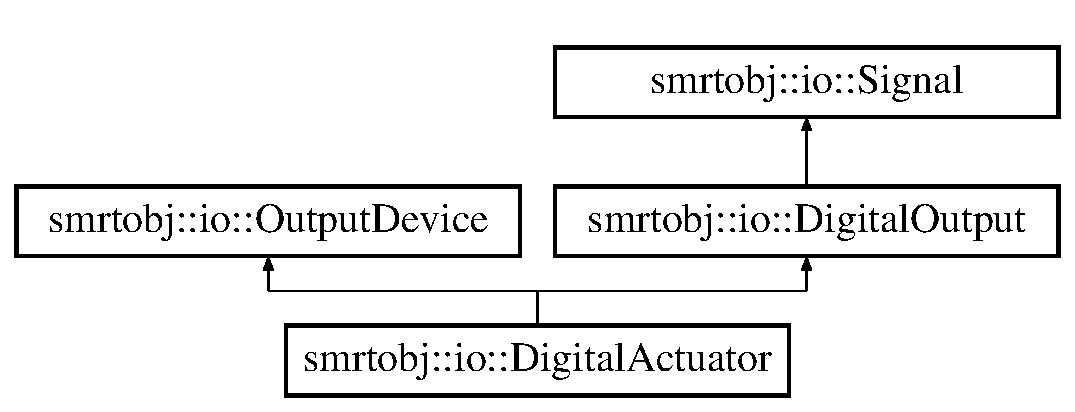
\includegraphics[height=3.000000cm]{classsmrtobj_1_1io_1_1_digital_actuator}
\end{center}
\end{figure}
\subsection*{Public Member Functions}
\begin{DoxyCompactItemize}
\item 
\hyperlink{classsmrtobj_1_1io_1_1_digital_actuator_ad144ef7a846aaf392b5701ba3646908a}{Digital\+Actuator} ()
\item 
\hyperlink{classsmrtobj_1_1io_1_1_digital_actuator_af969dc5c7e6f6a90bacc2d927b59dd5e}{Digital\+Actuator} (const \hyperlink{classsmrtobj_1_1io_1_1_digital_actuator}{Digital\+Actuator} \&a)
\item 
virtual \hyperlink{classsmrtobj_1_1io_1_1_digital_actuator_a8b53144b2fb3c24bc37635aa5a762506}{$\sim$\+Digital\+Actuator} ()
\item 
\hyperlink{classsmrtobj_1_1io_1_1_digital_actuator}{Digital\+Actuator} \& \hyperlink{classsmrtobj_1_1io_1_1_digital_actuator_a6a8ccda71f81c0951b49ce41f3ee9781}{operator=} (const \hyperlink{classsmrtobj_1_1io_1_1_digital_actuator}{Digital\+Actuator} \&a)
\item 
bool \hyperlink{classsmrtobj_1_1io_1_1_digital_actuator_a5566c8e9f190226f3b12ad1f2c198599}{init} (byte \hyperlink{classsmrtobj_1_1io_1_1_digital_output_aef26855d23bba50d3b47ec76443fe1c9}{pin}, bool negate=false)
\item 
virtual bool \hyperlink{classsmrtobj_1_1io_1_1_digital_actuator_a2264475c4969b42e95118e73579d4d74}{on} ()
\item 
virtual bool \hyperlink{classsmrtobj_1_1io_1_1_digital_actuator_aa5b6758d4bc05c9ae9ed666d62f65958}{off} ()
\end{DoxyCompactItemize}
\subsection*{Additional Inherited Members}


\subsection{Detailed Description}
The \hyperlink{classsmrtobj_1_1io_1_1_digital_actuator}{Digital\+Actuator} class models a generic actuator. It changes the output of a digital output to H\+I\+G\+H or L\+O\+W. Actuator can have two different state {\ttfamily O\+N} or {\ttfamily O\+F\+F} and works in {\ttfamily positive} (H\+I\+G\+H means O\+N and L\+O\+W means O\+F\+F) or negative (H\+I\+G\+H means O\+F\+F and L\+O\+W means O\+N) logic. 

Definition at line 29 of file digitalactuator.\+h.



\subsection{Constructor \& Destructor Documentation}
\hypertarget{classsmrtobj_1_1io_1_1_digital_actuator_ad144ef7a846aaf392b5701ba3646908a}{}\index{smrtobj\+::io\+::\+Digital\+Actuator@{smrtobj\+::io\+::\+Digital\+Actuator}!Digital\+Actuator@{Digital\+Actuator}}
\index{Digital\+Actuator@{Digital\+Actuator}!smrtobj\+::io\+::\+Digital\+Actuator@{smrtobj\+::io\+::\+Digital\+Actuator}}
\subsubsection[{Digital\+Actuator()}]{\setlength{\rightskip}{0pt plus 5cm}smrtobj\+::io\+::\+Digital\+Actuator\+::\+Digital\+Actuator (
\begin{DoxyParamCaption}
{}
\end{DoxyParamCaption}
)}\label{classsmrtobj_1_1io_1_1_digital_actuator_ad144ef7a846aaf392b5701ba3646908a}
Default Constructor. It initializes the state of the actuator to switched off and the output pin to 0. The actuator works in positive logic by default (H\+I\+G\+H\+: turn on, L\+O\+W\+: turn off). 

Definition at line 16 of file digitalactuator.\+cpp.

\hypertarget{classsmrtobj_1_1io_1_1_digital_actuator_af969dc5c7e6f6a90bacc2d927b59dd5e}{}\index{smrtobj\+::io\+::\+Digital\+Actuator@{smrtobj\+::io\+::\+Digital\+Actuator}!Digital\+Actuator@{Digital\+Actuator}}
\index{Digital\+Actuator@{Digital\+Actuator}!smrtobj\+::io\+::\+Digital\+Actuator@{smrtobj\+::io\+::\+Digital\+Actuator}}
\subsubsection[{Digital\+Actuator(const Digital\+Actuator \&a)}]{\setlength{\rightskip}{0pt plus 5cm}smrtobj\+::io\+::\+Digital\+Actuator\+::\+Digital\+Actuator (
\begin{DoxyParamCaption}
\item[{const {\bf Digital\+Actuator} \&}]{a}
\end{DoxyParamCaption}
)}\label{classsmrtobj_1_1io_1_1_digital_actuator_af969dc5c7e6f6a90bacc2d927b59dd5e}
Copy constructor.


\begin{DoxyParams}[1]{Parameters}
\mbox{\tt in}  & {\em a} & source digital actuator \\
\hline
\end{DoxyParams}


Definition at line 20 of file digitalactuator.\+cpp.

\hypertarget{classsmrtobj_1_1io_1_1_digital_actuator_a8b53144b2fb3c24bc37635aa5a762506}{}\index{smrtobj\+::io\+::\+Digital\+Actuator@{smrtobj\+::io\+::\+Digital\+Actuator}!````~Digital\+Actuator@{$\sim$\+Digital\+Actuator}}
\index{````~Digital\+Actuator@{$\sim$\+Digital\+Actuator}!smrtobj\+::io\+::\+Digital\+Actuator@{smrtobj\+::io\+::\+Digital\+Actuator}}
\subsubsection[{$\sim$\+Digital\+Actuator()}]{\setlength{\rightskip}{0pt plus 5cm}smrtobj\+::io\+::\+Digital\+Actuator\+::$\sim$\+Digital\+Actuator (
\begin{DoxyParamCaption}
{}
\end{DoxyParamCaption}
)\hspace{0.3cm}{\ttfamily [virtual]}}\label{classsmrtobj_1_1io_1_1_digital_actuator_a8b53144b2fb3c24bc37635aa5a762506}
Destructor. 

Definition at line 25 of file digitalactuator.\+cpp.



\subsection{Member Function Documentation}
\hypertarget{classsmrtobj_1_1io_1_1_digital_actuator_a5566c8e9f190226f3b12ad1f2c198599}{}\index{smrtobj\+::io\+::\+Digital\+Actuator@{smrtobj\+::io\+::\+Digital\+Actuator}!init@{init}}
\index{init@{init}!smrtobj\+::io\+::\+Digital\+Actuator@{smrtobj\+::io\+::\+Digital\+Actuator}}
\subsubsection[{init(byte pin, bool negate=false)}]{\setlength{\rightskip}{0pt plus 5cm}bool smrtobj\+::io\+::\+Digital\+Actuator\+::init (
\begin{DoxyParamCaption}
\item[{byte}]{pin, }
\item[{bool}]{negate = {\ttfamily false}}
\end{DoxyParamCaption}
)}\label{classsmrtobj_1_1io_1_1_digital_actuator_a5566c8e9f190226f3b12ad1f2c198599}
Initializes all attributes of the actuator and switches it off.


\begin{DoxyParams}[1]{Parameters}
\mbox{\tt in}  & {\em pin} & number of the output pin \\
\hline
\mbox{\tt in}  & {\em negate} & true if actuator works in negative logic, false otherwise\\
\hline
\end{DoxyParams}
\begin{DoxyReturn}{Returns}
true if there are errors, false otherwise 
\end{DoxyReturn}


Definition at line 38 of file digitalactuator.\+cpp.

\hypertarget{classsmrtobj_1_1io_1_1_digital_actuator_aa5b6758d4bc05c9ae9ed666d62f65958}{}\index{smrtobj\+::io\+::\+Digital\+Actuator@{smrtobj\+::io\+::\+Digital\+Actuator}!off@{off}}
\index{off@{off}!smrtobj\+::io\+::\+Digital\+Actuator@{smrtobj\+::io\+::\+Digital\+Actuator}}
\subsubsection[{off()}]{\setlength{\rightskip}{0pt plus 5cm}bool smrtobj\+::io\+::\+Digital\+Actuator\+::off (
\begin{DoxyParamCaption}
{}
\end{DoxyParamCaption}
)\hspace{0.3cm}{\ttfamily [virtual]}}\label{classsmrtobj_1_1io_1_1_digital_actuator_aa5b6758d4bc05c9ae9ed666d62f65958}
Switches the actuator off

\begin{DoxyReturn}{Returns}
true if there are no errors, false otherwise 
\end{DoxyReturn}


Implements \hyperlink{classsmrtobj_1_1io_1_1_output_device_a2700863f90da699cb82835ea6bb1f2f5}{smrtobj\+::io\+::\+Output\+Device}.



Definition at line 61 of file digitalactuator.\+cpp.

\hypertarget{classsmrtobj_1_1io_1_1_digital_actuator_a2264475c4969b42e95118e73579d4d74}{}\index{smrtobj\+::io\+::\+Digital\+Actuator@{smrtobj\+::io\+::\+Digital\+Actuator}!on@{on}}
\index{on@{on}!smrtobj\+::io\+::\+Digital\+Actuator@{smrtobj\+::io\+::\+Digital\+Actuator}}
\subsubsection[{on()}]{\setlength{\rightskip}{0pt plus 5cm}bool smrtobj\+::io\+::\+Digital\+Actuator\+::on (
\begin{DoxyParamCaption}
{}
\end{DoxyParamCaption}
)\hspace{0.3cm}{\ttfamily [virtual]}}\label{classsmrtobj_1_1io_1_1_digital_actuator_a2264475c4969b42e95118e73579d4d74}
Switches the actuator on

\begin{DoxyReturn}{Returns}
true if there are no errors, false otherwise 
\end{DoxyReturn}


Implements \hyperlink{classsmrtobj_1_1io_1_1_output_device_a9154253249a8e95d69fa9d4ade592049}{smrtobj\+::io\+::\+Output\+Device}.



Definition at line 48 of file digitalactuator.\+cpp.

\hypertarget{classsmrtobj_1_1io_1_1_digital_actuator_a6a8ccda71f81c0951b49ce41f3ee9781}{}\index{smrtobj\+::io\+::\+Digital\+Actuator@{smrtobj\+::io\+::\+Digital\+Actuator}!operator=@{operator=}}
\index{operator=@{operator=}!smrtobj\+::io\+::\+Digital\+Actuator@{smrtobj\+::io\+::\+Digital\+Actuator}}
\subsubsection[{operator=(const Digital\+Actuator \&a)}]{\setlength{\rightskip}{0pt plus 5cm}{\bf Digital\+Actuator} \& smrtobj\+::io\+::\+Digital\+Actuator\+::operator= (
\begin{DoxyParamCaption}
\item[{const {\bf Digital\+Actuator} \&}]{a}
\end{DoxyParamCaption}
)}\label{classsmrtobj_1_1io_1_1_digital_actuator_a6a8ccda71f81c0951b49ce41f3ee9781}
Override operator =


\begin{DoxyParams}[1]{Parameters}
\mbox{\tt in}  & {\em a} & source digital actuator\\
\hline
\end{DoxyParams}
\begin{DoxyReturn}{Returns}
reference to the destination digital actuator 
\end{DoxyReturn}


Definition at line 29 of file digitalactuator.\+cpp.



The documentation for this class was generated from the following files\+:\begin{DoxyCompactItemize}
\item 
libraries/\+Smrt\+Obj\+I\+O/src/actuator/\hyperlink{digitalactuator_8h}{digitalactuator.\+h}\item 
libraries/\+Smrt\+Obj\+I\+O/src/actuator/\hyperlink{digitalactuator_8cpp}{digitalactuator.\+cpp}\end{DoxyCompactItemize}

\hypertarget{classsmrtobj_1_1io_1_1_digital_input}{}\section{smrtobj\+:\+:io\+:\+:Digital\+Input Class Reference}
\label{classsmrtobj_1_1io_1_1_digital_input}\index{smrtobj\+::io\+::\+Digital\+Input@{smrtobj\+::io\+::\+Digital\+Input}}


{\ttfamily \#include $<$iosignal.\+h$>$}

Inheritance diagram for smrtobj\+:\+:io\+:\+:Digital\+Input\+:\begin{figure}[H]
\begin{center}
\leavevmode
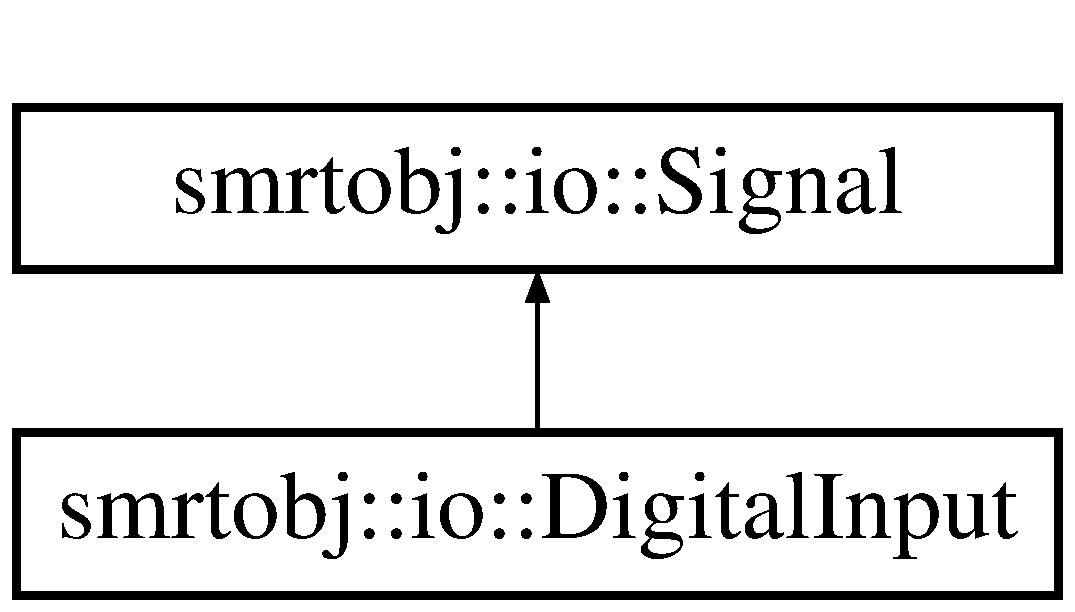
\includegraphics[height=2.000000cm]{classsmrtobj_1_1io_1_1_digital_input}
\end{center}
\end{figure}
\subsection*{Public Member Functions}
\begin{DoxyCompactItemize}
\item 
\hyperlink{classsmrtobj_1_1io_1_1_digital_input_af2ef9ec74d536240b0857f0de1c02796}{Digital\+Input} ()
\item 
\hyperlink{classsmrtobj_1_1io_1_1_digital_input_afe5da52de886356d5029b7fd15655c19}{Digital\+Input} (const \hyperlink{classsmrtobj_1_1io_1_1_digital_input}{Digital\+Input} \&o)
\item 
virtual \hyperlink{classsmrtobj_1_1io_1_1_digital_input_a35b580da1540a13d37eedb2344d95bf7}{$\sim$\+Digital\+Input} ()
\item 
\hyperlink{classsmrtobj_1_1io_1_1_digital_input}{Digital\+Input} \& \hyperlink{classsmrtobj_1_1io_1_1_digital_input_a609bdafe6cf1327b70fee98080a54dd5}{operator=} (const \hyperlink{classsmrtobj_1_1io_1_1_digital_input}{Digital\+Input} \&o)
\item 
byte \hyperlink{classsmrtobj_1_1io_1_1_digital_input_a89f92208f29c7ca20cdc35689c8aad6a}{type} ()
\item 
void \hyperlink{classsmrtobj_1_1io_1_1_digital_input_a71826ab0ec74668d3f3d5feec91f659d}{init} (byte \hyperlink{classsmrtobj_1_1io_1_1_digital_input_aa6bbdb4628b50d70084de992aaeee3ed}{pin}, bool pullup=false)
\item 
bool \hyperlink{classsmrtobj_1_1io_1_1_digital_input_a298b5554b20605d9265e225414299c1c}{value} ()
\item 
byte \hyperlink{classsmrtobj_1_1io_1_1_digital_input_aa6bbdb4628b50d70084de992aaeee3ed}{pin} ()
\item 
bool \hyperlink{classsmrtobj_1_1io_1_1_digital_input_a606e21b6c15a53bf5fe9aad68f997d38}{read} ()
\end{DoxyCompactItemize}
\subsection*{Additional Inherited Members}


\subsection{Detailed Description}
The \hyperlink{classsmrtobj_1_1io_1_1_digital_input}{Digital\+Input} class models a digital input. Using this, it is possible read the value from a specified digital pin, either H\+I\+G\+H or L\+O\+W. 

Definition at line 208 of file iosignal.\+h.



\subsection{Constructor \& Destructor Documentation}
\hypertarget{classsmrtobj_1_1io_1_1_digital_input_af2ef9ec74d536240b0857f0de1c02796}{}\index{smrtobj\+::io\+::\+Digital\+Input@{smrtobj\+::io\+::\+Digital\+Input}!Digital\+Input@{Digital\+Input}}
\index{Digital\+Input@{Digital\+Input}!smrtobj\+::io\+::\+Digital\+Input@{smrtobj\+::io\+::\+Digital\+Input}}
\subsubsection[{Digital\+Input()}]{\setlength{\rightskip}{0pt plus 5cm}smrtobj\+::io\+::\+Digital\+Input\+::\+Digital\+Input (
\begin{DoxyParamCaption}
{}
\end{DoxyParamCaption}
)}\label{classsmrtobj_1_1io_1_1_digital_input_af2ef9ec74d536240b0857f0de1c02796}
Default Constructor. It initializes the last value read to 0 and the pin number to 0. 

Definition at line 117 of file iosignal.\+cpp.

\hypertarget{classsmrtobj_1_1io_1_1_digital_input_afe5da52de886356d5029b7fd15655c19}{}\index{smrtobj\+::io\+::\+Digital\+Input@{smrtobj\+::io\+::\+Digital\+Input}!Digital\+Input@{Digital\+Input}}
\index{Digital\+Input@{Digital\+Input}!smrtobj\+::io\+::\+Digital\+Input@{smrtobj\+::io\+::\+Digital\+Input}}
\subsubsection[{Digital\+Input(const Digital\+Input \&o)}]{\setlength{\rightskip}{0pt plus 5cm}smrtobj\+::io\+::\+Digital\+Input\+::\+Digital\+Input (
\begin{DoxyParamCaption}
\item[{const {\bf Digital\+Input} \&}]{o}
\end{DoxyParamCaption}
)}\label{classsmrtobj_1_1io_1_1_digital_input_afe5da52de886356d5029b7fd15655c19}
Copy Constructor.


\begin{DoxyParams}[1]{Parameters}
\mbox{\tt in}  & {\em o} & source digital input \\
\hline
\end{DoxyParams}


Definition at line 122 of file iosignal.\+cpp.

\hypertarget{classsmrtobj_1_1io_1_1_digital_input_a35b580da1540a13d37eedb2344d95bf7}{}\index{smrtobj\+::io\+::\+Digital\+Input@{smrtobj\+::io\+::\+Digital\+Input}!````~Digital\+Input@{$\sim$\+Digital\+Input}}
\index{````~Digital\+Input@{$\sim$\+Digital\+Input}!smrtobj\+::io\+::\+Digital\+Input@{smrtobj\+::io\+::\+Digital\+Input}}
\subsubsection[{$\sim$\+Digital\+Input()}]{\setlength{\rightskip}{0pt plus 5cm}smrtobj\+::io\+::\+Digital\+Input\+::$\sim$\+Digital\+Input (
\begin{DoxyParamCaption}
{}
\end{DoxyParamCaption}
)\hspace{0.3cm}{\ttfamily [virtual]}}\label{classsmrtobj_1_1io_1_1_digital_input_a35b580da1540a13d37eedb2344d95bf7}
Destructor 

Definition at line 128 of file iosignal.\+cpp.



\subsection{Member Function Documentation}
\hypertarget{classsmrtobj_1_1io_1_1_digital_input_a71826ab0ec74668d3f3d5feec91f659d}{}\index{smrtobj\+::io\+::\+Digital\+Input@{smrtobj\+::io\+::\+Digital\+Input}!init@{init}}
\index{init@{init}!smrtobj\+::io\+::\+Digital\+Input@{smrtobj\+::io\+::\+Digital\+Input}}
\subsubsection[{init(byte pin, bool pullup=false)}]{\setlength{\rightskip}{0pt plus 5cm}void smrtobj\+::io\+::\+Digital\+Input\+::init (
\begin{DoxyParamCaption}
\item[{byte}]{pin, }
\item[{bool}]{pullup = {\ttfamily false}}
\end{DoxyParamCaption}
)}\label{classsmrtobj_1_1io_1_1_digital_input_a71826ab0ec74668d3f3d5feec91f659d}
Opens the pin in input mode. It is possible use internal pull up resistor.~\newline
The Atmega microcontroller on the Arduino has internal pull-\/up resistors (resistors that connect to power internally) that you can access. If you prefer to use these instead of external pull-\/up resistors, you can use pullup argument to true.


\begin{DoxyParams}[1]{Parameters}
\mbox{\tt in}  & {\em pin} & number of the input pin \\
\hline
\mbox{\tt in}  & {\em pullup} & use internal pull up resistor. Default value is false \\
\hline
\end{DoxyParams}


Definition at line 141 of file iosignal.\+cpp.

\hypertarget{classsmrtobj_1_1io_1_1_digital_input_a609bdafe6cf1327b70fee98080a54dd5}{}\index{smrtobj\+::io\+::\+Digital\+Input@{smrtobj\+::io\+::\+Digital\+Input}!operator=@{operator=}}
\index{operator=@{operator=}!smrtobj\+::io\+::\+Digital\+Input@{smrtobj\+::io\+::\+Digital\+Input}}
\subsubsection[{operator=(const Digital\+Input \&o)}]{\setlength{\rightskip}{0pt plus 5cm}{\bf Digital\+Input} \& smrtobj\+::io\+::\+Digital\+Input\+::operator= (
\begin{DoxyParamCaption}
\item[{const {\bf Digital\+Input} \&}]{o}
\end{DoxyParamCaption}
)}\label{classsmrtobj_1_1io_1_1_digital_input_a609bdafe6cf1327b70fee98080a54dd5}
Override operator =


\begin{DoxyParams}[1]{Parameters}
\mbox{\tt in}  & {\em o} & source digital input\\
\hline
\end{DoxyParams}
\begin{DoxyReturn}{Returns}
reference to the destination digital input object 
\end{DoxyReturn}


Definition at line 132 of file iosignal.\+cpp.

\hypertarget{classsmrtobj_1_1io_1_1_digital_input_aa6bbdb4628b50d70084de992aaeee3ed}{}\index{smrtobj\+::io\+::\+Digital\+Input@{smrtobj\+::io\+::\+Digital\+Input}!pin@{pin}}
\index{pin@{pin}!smrtobj\+::io\+::\+Digital\+Input@{smrtobj\+::io\+::\+Digital\+Input}}
\subsubsection[{pin()}]{\setlength{\rightskip}{0pt plus 5cm}byte smrtobj\+::io\+::\+Digital\+Input\+::pin (
\begin{DoxyParamCaption}
{}
\end{DoxyParamCaption}
)\hspace{0.3cm}{\ttfamily [inline]}}\label{classsmrtobj_1_1io_1_1_digital_input_aa6bbdb4628b50d70084de992aaeee3ed}
Gets the number of the input pin.

\begin{DoxyReturn}{Returns}
pin number 
\end{DoxyReturn}


Definition at line 272 of file iosignal.\+h.

\hypertarget{classsmrtobj_1_1io_1_1_digital_input_a606e21b6c15a53bf5fe9aad68f997d38}{}\index{smrtobj\+::io\+::\+Digital\+Input@{smrtobj\+::io\+::\+Digital\+Input}!read@{read}}
\index{read@{read}!smrtobj\+::io\+::\+Digital\+Input@{smrtobj\+::io\+::\+Digital\+Input}}
\subsubsection[{read()}]{\setlength{\rightskip}{0pt plus 5cm}bool smrtobj\+::io\+::\+Digital\+Input\+::read (
\begin{DoxyParamCaption}
{}
\end{DoxyParamCaption}
)}\label{classsmrtobj_1_1io_1_1_digital_input_a606e21b6c15a53bf5fe9aad68f997d38}
Reads value from the digital input

\begin{DoxyReturn}{Returns}
value, it can be H\+I\+G\+H or L\+O\+W 
\end{DoxyReturn}


Definition at line 157 of file iosignal.\+cpp.

\hypertarget{classsmrtobj_1_1io_1_1_digital_input_a89f92208f29c7ca20cdc35689c8aad6a}{}\index{smrtobj\+::io\+::\+Digital\+Input@{smrtobj\+::io\+::\+Digital\+Input}!type@{type}}
\index{type@{type}!smrtobj\+::io\+::\+Digital\+Input@{smrtobj\+::io\+::\+Digital\+Input}}
\subsubsection[{type()}]{\setlength{\rightskip}{0pt plus 5cm}byte smrtobj\+::io\+::\+Digital\+Input\+::type (
\begin{DoxyParamCaption}
{}
\end{DoxyParamCaption}
)\hspace{0.3cm}{\ttfamily [inline]}, {\ttfamily [virtual]}}\label{classsmrtobj_1_1io_1_1_digital_input_a89f92208f29c7ca20cdc35689c8aad6a}
Gets the type of the interface according to \#smrtobj\+::\+Signal\+::\+\_\+type enum

\begin{DoxyReturn}{Returns}
type of the interface 
\end{DoxyReturn}


Implements \hyperlink{classsmrtobj_1_1io_1_1_signal_a38cd36f413f1ad2213684e4364ac4270}{smrtobj\+::io\+::\+Signal}.



Definition at line 246 of file iosignal.\+h.

\hypertarget{classsmrtobj_1_1io_1_1_digital_input_a298b5554b20605d9265e225414299c1c}{}\index{smrtobj\+::io\+::\+Digital\+Input@{smrtobj\+::io\+::\+Digital\+Input}!value@{value}}
\index{value@{value}!smrtobj\+::io\+::\+Digital\+Input@{smrtobj\+::io\+::\+Digital\+Input}}
\subsubsection[{value()}]{\setlength{\rightskip}{0pt plus 5cm}bool smrtobj\+::io\+::\+Digital\+Input\+::value (
\begin{DoxyParamCaption}
{}
\end{DoxyParamCaption}
)\hspace{0.3cm}{\ttfamily [inline]}}\label{classsmrtobj_1_1io_1_1_digital_input_a298b5554b20605d9265e225414299c1c}
Gets the last value read.

\begin{DoxyReturn}{Returns}
last value read (true if H\+I\+G\+H, false if L\+O\+W or input has not been opened) 
\end{DoxyReturn}


Definition at line 265 of file iosignal.\+h.



The documentation for this class was generated from the following files\+:\begin{DoxyCompactItemize}
\item 
libraries/\+Smrt\+Obj\+I\+O/src/\hyperlink{iosignal_8h}{iosignal.\+h}\item 
libraries/\+Smrt\+Obj\+I\+O/src/\hyperlink{iosignal_8cpp}{iosignal.\+cpp}\end{DoxyCompactItemize}

\hypertarget{classsmrtobj_1_1io_1_1_digital_output}{}\section{smrtobj\+:\+:io\+:\+:Digital\+Output Class Reference}
\label{classsmrtobj_1_1io_1_1_digital_output}\index{smrtobj\+::io\+::\+Digital\+Output@{smrtobj\+::io\+::\+Digital\+Output}}


{\ttfamily \#include $<$iosignal.\+h$>$}

Inheritance diagram for smrtobj\+:\+:io\+:\+:Digital\+Output\+:\begin{figure}[H]
\begin{center}
\leavevmode
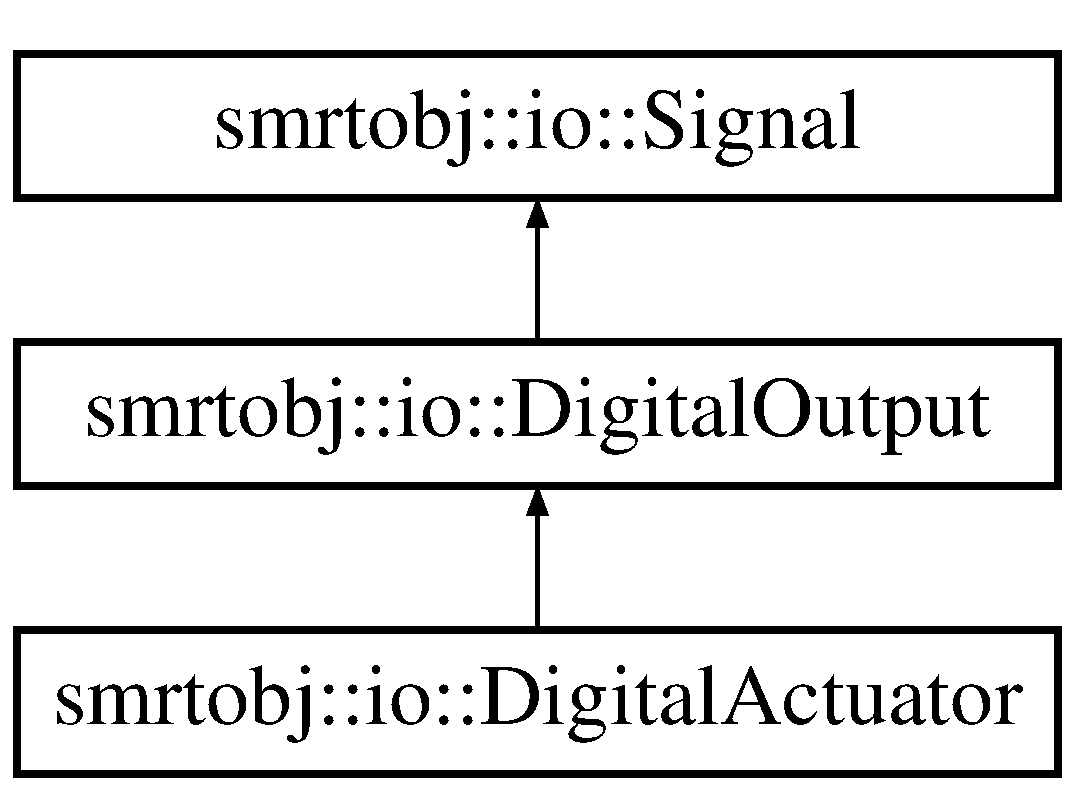
\includegraphics[height=3.000000cm]{classsmrtobj_1_1io_1_1_digital_output}
\end{center}
\end{figure}
\subsection*{Public Member Functions}
\begin{DoxyCompactItemize}
\item 
\hyperlink{classsmrtobj_1_1io_1_1_digital_output_a4f8b427dd834072bc274cfe8fd44f1ac}{Digital\+Output} ()
\item 
\hyperlink{classsmrtobj_1_1io_1_1_digital_output_a6ccc224b58e5ab04c327b3fd62f592ef}{Digital\+Output} (const \hyperlink{classsmrtobj_1_1io_1_1_digital_output}{Digital\+Output} \&o)
\item 
virtual \hyperlink{classsmrtobj_1_1io_1_1_digital_output_a43e0743797dcbdf400340a94c38c8da0}{$\sim$\+Digital\+Output} ()
\item 
\hyperlink{classsmrtobj_1_1io_1_1_digital_output}{Digital\+Output} \& \hyperlink{classsmrtobj_1_1io_1_1_digital_output_ae7d37f28cc4e9db61f6853cccfe4f6c5}{operator=} (const \hyperlink{classsmrtobj_1_1io_1_1_digital_output}{Digital\+Output} \&o)
\item 
byte \hyperlink{classsmrtobj_1_1io_1_1_digital_output_a9c9e665bb38c2c8164cfce1a3ce94dcc}{type} ()
\item 
void \hyperlink{classsmrtobj_1_1io_1_1_digital_output_a62cc30d2d5e3ea1d11bfd5b3a5b59312}{init} (byte \hyperlink{classsmrtobj_1_1io_1_1_digital_output_aef26855d23bba50d3b47ec76443fe1c9}{pin})
\item 
bool \hyperlink{classsmrtobj_1_1io_1_1_digital_output_a0e7ee22a168f81b438fd513ceab22e27}{value} ()
\item 
byte \hyperlink{classsmrtobj_1_1io_1_1_digital_output_aef26855d23bba50d3b47ec76443fe1c9}{pin} ()
\item 
bool \hyperlink{classsmrtobj_1_1io_1_1_digital_output_a12fab5b3bd5012fa042c6d3cb6ab2663}{write} (bool \hyperlink{classsmrtobj_1_1io_1_1_digital_output_a0e7ee22a168f81b438fd513ceab22e27}{value})
\end{DoxyCompactItemize}
\subsection*{Additional Inherited Members}


\subsection{Detailed Description}
The \hyperlink{classsmrtobj_1_1io_1_1_digital_output}{Digital\+Output} class models an digital output. Output value can be {\bfseries H\+I\+G\+H} or {\bfseries L\+O\+W}. The last value written is stored in an internal variable. The default output pin is 0. 

Definition at line 26 of file iosignal.\+h.



\subsection{Constructor \& Destructor Documentation}
\hypertarget{classsmrtobj_1_1io_1_1_digital_output_a4f8b427dd834072bc274cfe8fd44f1ac}{}\index{smrtobj\+::io\+::\+Digital\+Output@{smrtobj\+::io\+::\+Digital\+Output}!Digital\+Output@{Digital\+Output}}
\index{Digital\+Output@{Digital\+Output}!smrtobj\+::io\+::\+Digital\+Output@{smrtobj\+::io\+::\+Digital\+Output}}
\subsubsection[{Digital\+Output()}]{\setlength{\rightskip}{0pt plus 5cm}smrtobj\+::io\+::\+Digital\+Output\+::\+Digital\+Output (
\begin{DoxyParamCaption}
{}
\end{DoxyParamCaption}
)}\label{classsmrtobj_1_1io_1_1_digital_output_a4f8b427dd834072bc274cfe8fd44f1ac}
Default Constructor. It initializes the last value written to L\+O\+W and the pin number to 0. 

Definition at line 19 of file iosignal.\+cpp.

\hypertarget{classsmrtobj_1_1io_1_1_digital_output_a6ccc224b58e5ab04c327b3fd62f592ef}{}\index{smrtobj\+::io\+::\+Digital\+Output@{smrtobj\+::io\+::\+Digital\+Output}!Digital\+Output@{Digital\+Output}}
\index{Digital\+Output@{Digital\+Output}!smrtobj\+::io\+::\+Digital\+Output@{smrtobj\+::io\+::\+Digital\+Output}}
\subsubsection[{Digital\+Output(const Digital\+Output \&o)}]{\setlength{\rightskip}{0pt plus 5cm}smrtobj\+::io\+::\+Digital\+Output\+::\+Digital\+Output (
\begin{DoxyParamCaption}
\item[{const {\bf Digital\+Output} \&}]{o}
\end{DoxyParamCaption}
)}\label{classsmrtobj_1_1io_1_1_digital_output_a6ccc224b58e5ab04c327b3fd62f592ef}
Copy Constructor.


\begin{DoxyParams}[1]{Parameters}
\mbox{\tt in}  & {\em o} & source digital output \\
\hline
\end{DoxyParams}


Definition at line 24 of file iosignal.\+cpp.

\hypertarget{classsmrtobj_1_1io_1_1_digital_output_a43e0743797dcbdf400340a94c38c8da0}{}\index{smrtobj\+::io\+::\+Digital\+Output@{smrtobj\+::io\+::\+Digital\+Output}!````~Digital\+Output@{$\sim$\+Digital\+Output}}
\index{````~Digital\+Output@{$\sim$\+Digital\+Output}!smrtobj\+::io\+::\+Digital\+Output@{smrtobj\+::io\+::\+Digital\+Output}}
\subsubsection[{$\sim$\+Digital\+Output()}]{\setlength{\rightskip}{0pt plus 5cm}smrtobj\+::io\+::\+Digital\+Output\+::$\sim$\+Digital\+Output (
\begin{DoxyParamCaption}
{}
\end{DoxyParamCaption}
)\hspace{0.3cm}{\ttfamily [virtual]}}\label{classsmrtobj_1_1io_1_1_digital_output_a43e0743797dcbdf400340a94c38c8da0}
Destructor. 

Definition at line 30 of file iosignal.\+cpp.



\subsection{Member Function Documentation}
\hypertarget{classsmrtobj_1_1io_1_1_digital_output_a62cc30d2d5e3ea1d11bfd5b3a5b59312}{}\index{smrtobj\+::io\+::\+Digital\+Output@{smrtobj\+::io\+::\+Digital\+Output}!init@{init}}
\index{init@{init}!smrtobj\+::io\+::\+Digital\+Output@{smrtobj\+::io\+::\+Digital\+Output}}
\subsubsection[{init(byte pin)}]{\setlength{\rightskip}{0pt plus 5cm}void smrtobj\+::io\+::\+Digital\+Output\+::init (
\begin{DoxyParamCaption}
\item[{byte}]{pin}
\end{DoxyParamCaption}
)}\label{classsmrtobj_1_1io_1_1_digital_output_a62cc30d2d5e3ea1d11bfd5b3a5b59312}
Opens the pin and initializes the digital output.


\begin{DoxyParams}[1]{Parameters}
\mbox{\tt in}  & {\em pin} & number of the output pin \\
\hline
\end{DoxyParams}


Definition at line 43 of file iosignal.\+cpp.

\hypertarget{classsmrtobj_1_1io_1_1_digital_output_ae7d37f28cc4e9db61f6853cccfe4f6c5}{}\index{smrtobj\+::io\+::\+Digital\+Output@{smrtobj\+::io\+::\+Digital\+Output}!operator=@{operator=}}
\index{operator=@{operator=}!smrtobj\+::io\+::\+Digital\+Output@{smrtobj\+::io\+::\+Digital\+Output}}
\subsubsection[{operator=(const Digital\+Output \&o)}]{\setlength{\rightskip}{0pt plus 5cm}{\bf Digital\+Output} \& smrtobj\+::io\+::\+Digital\+Output\+::operator= (
\begin{DoxyParamCaption}
\item[{const {\bf Digital\+Output} \&}]{o}
\end{DoxyParamCaption}
)}\label{classsmrtobj_1_1io_1_1_digital_output_ae7d37f28cc4e9db61f6853cccfe4f6c5}
Override operator =


\begin{DoxyParams}[1]{Parameters}
\mbox{\tt in}  & {\em o} & source digital output\\
\hline
\end{DoxyParams}
\begin{DoxyReturn}{Returns}
reference to the destination digital output 
\end{DoxyReturn}


Definition at line 34 of file iosignal.\+cpp.

\hypertarget{classsmrtobj_1_1io_1_1_digital_output_aef26855d23bba50d3b47ec76443fe1c9}{}\index{smrtobj\+::io\+::\+Digital\+Output@{smrtobj\+::io\+::\+Digital\+Output}!pin@{pin}}
\index{pin@{pin}!smrtobj\+::io\+::\+Digital\+Output@{smrtobj\+::io\+::\+Digital\+Output}}
\subsubsection[{pin()}]{\setlength{\rightskip}{0pt plus 5cm}byte smrtobj\+::io\+::\+Digital\+Output\+::pin (
\begin{DoxyParamCaption}
{}
\end{DoxyParamCaption}
)\hspace{0.3cm}{\ttfamily [inline]}}\label{classsmrtobj_1_1io_1_1_digital_output_aef26855d23bba50d3b47ec76443fe1c9}
Gets the number of the output pin.

\begin{DoxyReturn}{Returns}
pin number 
\end{DoxyReturn}


Definition at line 85 of file iosignal.\+h.

\hypertarget{classsmrtobj_1_1io_1_1_digital_output_a9c9e665bb38c2c8164cfce1a3ce94dcc}{}\index{smrtobj\+::io\+::\+Digital\+Output@{smrtobj\+::io\+::\+Digital\+Output}!type@{type}}
\index{type@{type}!smrtobj\+::io\+::\+Digital\+Output@{smrtobj\+::io\+::\+Digital\+Output}}
\subsubsection[{type()}]{\setlength{\rightskip}{0pt plus 5cm}byte smrtobj\+::io\+::\+Digital\+Output\+::type (
\begin{DoxyParamCaption}
{}
\end{DoxyParamCaption}
)\hspace{0.3cm}{\ttfamily [inline]}, {\ttfamily [virtual]}}\label{classsmrtobj_1_1io_1_1_digital_output_a9c9e665bb38c2c8164cfce1a3ce94dcc}
Gets the type of the interface according to \#smrtobj\+::\+Signal\+::\+\_\+type enum

\begin{DoxyReturn}{Returns}
type of the interface 
\end{DoxyReturn}


Implements \hyperlink{classsmrtobj_1_1io_1_1_signal_a38cd36f413f1ad2213684e4364ac4270}{smrtobj\+::io\+::\+Signal}.



Definition at line 63 of file iosignal.\+h.

\hypertarget{classsmrtobj_1_1io_1_1_digital_output_a0e7ee22a168f81b438fd513ceab22e27}{}\index{smrtobj\+::io\+::\+Digital\+Output@{smrtobj\+::io\+::\+Digital\+Output}!value@{value}}
\index{value@{value}!smrtobj\+::io\+::\+Digital\+Output@{smrtobj\+::io\+::\+Digital\+Output}}
\subsubsection[{value()}]{\setlength{\rightskip}{0pt plus 5cm}bool smrtobj\+::io\+::\+Digital\+Output\+::value (
\begin{DoxyParamCaption}
{}
\end{DoxyParamCaption}
)\hspace{0.3cm}{\ttfamily [inline]}}\label{classsmrtobj_1_1io_1_1_digital_output_a0e7ee22a168f81b438fd513ceab22e27}
Gets the last value written.

\begin{DoxyReturn}{Returns}
last value written 
\end{DoxyReturn}


Definition at line 78 of file iosignal.\+h.

\hypertarget{classsmrtobj_1_1io_1_1_digital_output_a12fab5b3bd5012fa042c6d3cb6ab2663}{}\index{smrtobj\+::io\+::\+Digital\+Output@{smrtobj\+::io\+::\+Digital\+Output}!write@{write}}
\index{write@{write}!smrtobj\+::io\+::\+Digital\+Output@{smrtobj\+::io\+::\+Digital\+Output}}
\subsubsection[{write(bool value)}]{\setlength{\rightskip}{0pt plus 5cm}bool smrtobj\+::io\+::\+Digital\+Output\+::write (
\begin{DoxyParamCaption}
\item[{bool}]{value}
\end{DoxyParamCaption}
)}\label{classsmrtobj_1_1io_1_1_digital_output_a12fab5b3bd5012fa042c6d3cb6ab2663}
Writes value on the digital output


\begin{DoxyParams}[1]{Parameters}
\mbox{\tt in}  & {\em value} & digital value. It can be L\+O\+W or H\+I\+G\+H\\
\hline
\end{DoxyParams}
\begin{DoxyReturn}{Returns}
false if digital output not initialized yet 
\end{DoxyReturn}


Definition at line 50 of file iosignal.\+cpp.



The documentation for this class was generated from the following files\+:\begin{DoxyCompactItemize}
\item 
libraries/\+Smrt\+Obj\+I\+O/src/\hyperlink{iosignal_8h}{iosignal.\+h}\item 
libraries/\+Smrt\+Obj\+I\+O/src/\hyperlink{iosignal_8cpp}{iosignal.\+cpp}\end{DoxyCompactItemize}

\hypertarget{classsmrtobj_1_1i2c_1_1_d_s130_r_t_c}{}\section{smrtobj\+:\+:i2c\+:\+:D\+S130\+R\+T\+C Class Reference}
\label{classsmrtobj_1_1i2c_1_1_d_s130_r_t_c}\index{smrtobj\+::i2c\+::\+D\+S130\+R\+T\+C@{smrtobj\+::i2c\+::\+D\+S130\+R\+T\+C}}


{\ttfamily \#include $<$D\+S130\+R\+T\+C.\+h$>$}

Inheritance diagram for smrtobj\+:\+:i2c\+:\+:D\+S130\+R\+T\+C\+:\begin{figure}[H]
\begin{center}
\leavevmode
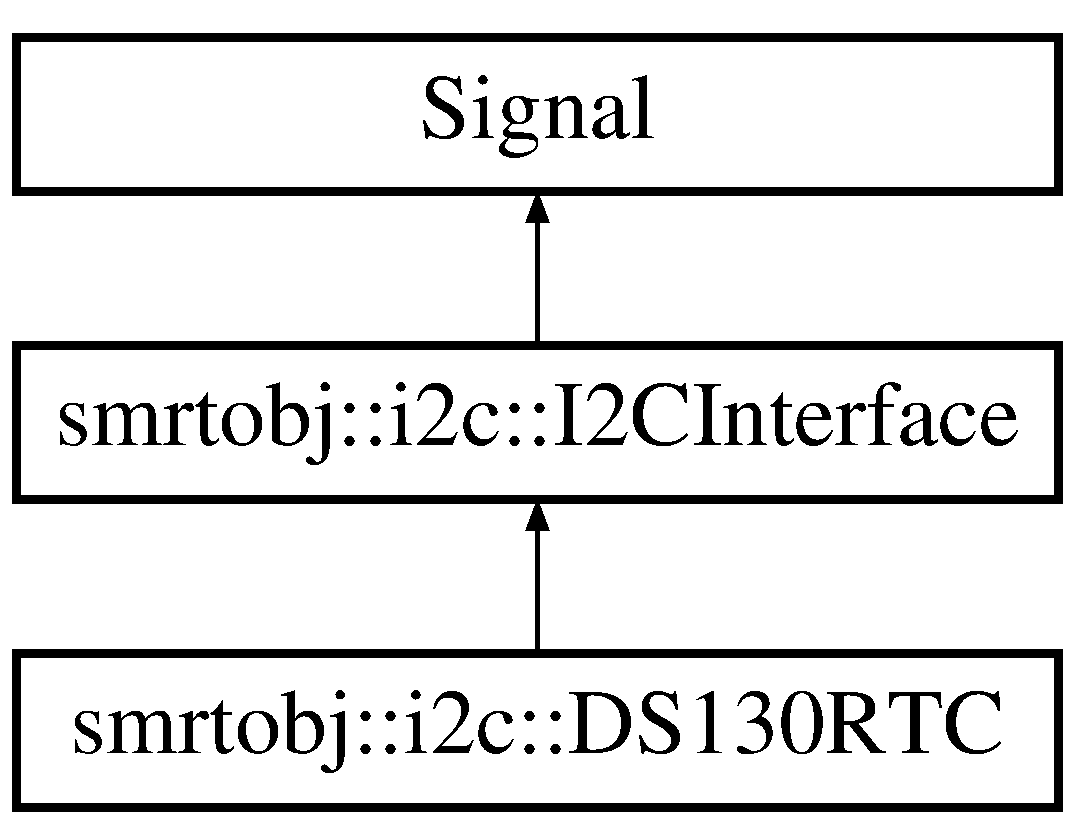
\includegraphics[height=3.000000cm]{classsmrtobj_1_1i2c_1_1_d_s130_r_t_c}
\end{center}
\end{figure}
\subsection*{Public Types}
\begin{DoxyCompactItemize}
\item 
enum \hyperlink{classsmrtobj_1_1i2c_1_1_d_s130_r_t_c_abd82e4e74a39bcb7a637ba90fc7dcce9}{\+\_\+device\+\_\+address} \{ {\bfseries D\+E\+V\+I\+C\+E\+\_\+\+A\+D\+D\+R\+E\+S\+S} = 0x68
 \}
\end{DoxyCompactItemize}
\subsection*{Public Member Functions}
\begin{DoxyCompactItemize}
\item 
\hyperlink{classsmrtobj_1_1i2c_1_1_d_s130_r_t_c_a1193dff2a364288f290e0fe3635c0cb6}{D\+S130\+R\+T\+C} ()
\item 
\hyperlink{classsmrtobj_1_1i2c_1_1_d_s130_r_t_c_a60a524983714ba79ec0cce24065c48ea}{D\+S130\+R\+T\+C} (const \hyperlink{classsmrtobj_1_1i2c_1_1_d_s130_r_t_c}{D\+S130\+R\+T\+C} \&d)
\item 
virtual \hyperlink{classsmrtobj_1_1i2c_1_1_d_s130_r_t_c_ac55df67fb47b399a26f3afada798674d}{$\sim$\+D\+S130\+R\+T\+C} ()
\item 
\hyperlink{classsmrtobj_1_1i2c_1_1_d_s130_r_t_c}{D\+S130\+R\+T\+C} \& \hyperlink{classsmrtobj_1_1i2c_1_1_d_s130_r_t_c_a3b041b1c4010942f43c164889fbc55ef}{operator=} (const \hyperlink{classsmrtobj_1_1i2c_1_1_d_s130_r_t_c}{D\+S130\+R\+T\+C} \&d)
\item 
virtual bool \hyperlink{classsmrtobj_1_1i2c_1_1_d_s130_r_t_c_aef59c049dbca2d78877e607e8009452c}{initialize} ()
\item 
virtual bool \hyperlink{classsmrtobj_1_1i2c_1_1_d_s130_r_t_c_ad8630568cd75431db924e2e723ebfcb4}{is\+Connected} ()
\item 
virtual bool \hyperlink{classsmrtobj_1_1i2c_1_1_d_s130_r_t_c_afc3af98fb550808741d738655ce642d1}{read} ()
\item 
bool \hyperlink{classsmrtobj_1_1i2c_1_1_d_s130_r_t_c_a3948a04b2efbb900ca2ec8a9ebd6dd79}{write} (time\+\_\+t t)
\item 
time\+\_\+t \hyperlink{classsmrtobj_1_1i2c_1_1_d_s130_r_t_c_aa83e66e3af3251924b7411daa55ce759}{time} ()
\end{DoxyCompactItemize}
\subsection*{Additional Inherited Members}


\subsection{Detailed Description}
Class \hyperlink{classsmrtobj_1_1i2c_1_1_d_s130_r_t_c}{D\+S130\+R\+T\+C} models the D\+S130 R\+T\+C device. The D\+S1307 serial real-\/time clock (R\+T\+C) is a low-\/power, full binary-\/coded decimal (B\+C\+D) clock/calendar plus 56 bytes of N\+V S\+R\+A\+M. Address and data are transferred serially through an I2\+C, bidirectional bus. The clock/calendar provides seconds, minutes, hours, day, date, month, and year information. The end of the month date is automatically adjusted for months with fewer than 31 days, including corrections for leap year. The clock operates in either the 24-\/hour or 12-\/hour format with A\+M/\+P\+M indicator. The D\+S1307 has a built-\/in power-\/sense circuit that detects power failures and automatically switches to the backup supply. Timekeeping operation continues while the part operates from the backup supply.

The contents of the time and calendar registers are in the B\+C\+D format. The day-\/of-\/week register increments at midnight. Values that correspond to the day of week are user defined but must be sequential (i.\+e., if 1 equals Sunday, then 2 equals Monday, and so on.) 

Definition at line 33 of file D\+S130\+R\+T\+C.\+h.



\subsection{Member Enumeration Documentation}
\hypertarget{classsmrtobj_1_1i2c_1_1_d_s130_r_t_c_abd82e4e74a39bcb7a637ba90fc7dcce9}{}\index{smrtobj\+::i2c\+::\+D\+S130\+R\+T\+C@{smrtobj\+::i2c\+::\+D\+S130\+R\+T\+C}!\+\_\+device\+\_\+address@{\+\_\+device\+\_\+address}}
\index{\+\_\+device\+\_\+address@{\+\_\+device\+\_\+address}!smrtobj\+::i2c\+::\+D\+S130\+R\+T\+C@{smrtobj\+::i2c\+::\+D\+S130\+R\+T\+C}}
\subsubsection[{\+\_\+device\+\_\+address}]{\setlength{\rightskip}{0pt plus 5cm}enum {\bf smrtobj\+::i2c\+::\+D\+S130\+R\+T\+C\+::\+\_\+device\+\_\+address}}\label{classsmrtobj_1_1i2c_1_1_d_s130_r_t_c_abd82e4e74a39bcb7a637ba90fc7dcce9}
Device address used by default 

Definition at line 39 of file D\+S130\+R\+T\+C.\+h.



\subsection{Constructor \& Destructor Documentation}
\hypertarget{classsmrtobj_1_1i2c_1_1_d_s130_r_t_c_a1193dff2a364288f290e0fe3635c0cb6}{}\index{smrtobj\+::i2c\+::\+D\+S130\+R\+T\+C@{smrtobj\+::i2c\+::\+D\+S130\+R\+T\+C}!D\+S130\+R\+T\+C@{D\+S130\+R\+T\+C}}
\index{D\+S130\+R\+T\+C@{D\+S130\+R\+T\+C}!smrtobj\+::i2c\+::\+D\+S130\+R\+T\+C@{smrtobj\+::i2c\+::\+D\+S130\+R\+T\+C}}
\subsubsection[{D\+S130\+R\+T\+C()}]{\setlength{\rightskip}{0pt plus 5cm}smrtobj\+::i2c\+::\+D\+S130\+R\+T\+C\+::\+D\+S130\+R\+T\+C (
\begin{DoxyParamCaption}
{}
\end{DoxyParamCaption}
)}\label{classsmrtobj_1_1i2c_1_1_d_s130_r_t_c_a1193dff2a364288f290e0fe3635c0cb6}
Default Constructor. 

Definition at line 15 of file D\+S130\+R\+T\+C.\+cpp.

\hypertarget{classsmrtobj_1_1i2c_1_1_d_s130_r_t_c_a60a524983714ba79ec0cce24065c48ea}{}\index{smrtobj\+::i2c\+::\+D\+S130\+R\+T\+C@{smrtobj\+::i2c\+::\+D\+S130\+R\+T\+C}!D\+S130\+R\+T\+C@{D\+S130\+R\+T\+C}}
\index{D\+S130\+R\+T\+C@{D\+S130\+R\+T\+C}!smrtobj\+::i2c\+::\+D\+S130\+R\+T\+C@{smrtobj\+::i2c\+::\+D\+S130\+R\+T\+C}}
\subsubsection[{D\+S130\+R\+T\+C(const D\+S130\+R\+T\+C \&d)}]{\setlength{\rightskip}{0pt plus 5cm}smrtobj\+::i2c\+::\+D\+S130\+R\+T\+C\+::\+D\+S130\+R\+T\+C (
\begin{DoxyParamCaption}
\item[{const {\bf D\+S130\+R\+T\+C} \&}]{d}
\end{DoxyParamCaption}
)}\label{classsmrtobj_1_1i2c_1_1_d_s130_r_t_c_a60a524983714ba79ec0cce24065c48ea}
Copy Constructor.


\begin{DoxyParams}[1]{Parameters}
\mbox{\tt in}  & {\em d} & I2\+C device object \\
\hline
\end{DoxyParams}


Definition at line 20 of file D\+S130\+R\+T\+C.\+cpp.

\hypertarget{classsmrtobj_1_1i2c_1_1_d_s130_r_t_c_ac55df67fb47b399a26f3afada798674d}{}\index{smrtobj\+::i2c\+::\+D\+S130\+R\+T\+C@{smrtobj\+::i2c\+::\+D\+S130\+R\+T\+C}!````~D\+S130\+R\+T\+C@{$\sim$\+D\+S130\+R\+T\+C}}
\index{````~D\+S130\+R\+T\+C@{$\sim$\+D\+S130\+R\+T\+C}!smrtobj\+::i2c\+::\+D\+S130\+R\+T\+C@{smrtobj\+::i2c\+::\+D\+S130\+R\+T\+C}}
\subsubsection[{$\sim$\+D\+S130\+R\+T\+C()}]{\setlength{\rightskip}{0pt plus 5cm}smrtobj\+::i2c\+::\+D\+S130\+R\+T\+C\+::$\sim$\+D\+S130\+R\+T\+C (
\begin{DoxyParamCaption}
{}
\end{DoxyParamCaption}
)\hspace{0.3cm}{\ttfamily [virtual]}}\label{classsmrtobj_1_1i2c_1_1_d_s130_r_t_c_ac55df67fb47b399a26f3afada798674d}
Destructor. 

Definition at line 25 of file D\+S130\+R\+T\+C.\+cpp.



\subsection{Member Function Documentation}
\hypertarget{classsmrtobj_1_1i2c_1_1_d_s130_r_t_c_aef59c049dbca2d78877e607e8009452c}{}\index{smrtobj\+::i2c\+::\+D\+S130\+R\+T\+C@{smrtobj\+::i2c\+::\+D\+S130\+R\+T\+C}!initialize@{initialize}}
\index{initialize@{initialize}!smrtobj\+::i2c\+::\+D\+S130\+R\+T\+C@{smrtobj\+::i2c\+::\+D\+S130\+R\+T\+C}}
\subsubsection[{initialize()}]{\setlength{\rightskip}{0pt plus 5cm}bool smrtobj\+::i2c\+::\+D\+S130\+R\+T\+C\+::initialize (
\begin{DoxyParamCaption}
{}
\end{DoxyParamCaption}
)\hspace{0.3cm}{\ttfamily [virtual]}}\label{classsmrtobj_1_1i2c_1_1_d_s130_r_t_c_aef59c049dbca2d78877e607e8009452c}
Starts I2\+C communications. For this device, this function does nothing.

\begin{DoxyReturn}{Returns}
always true 
\end{DoxyReturn}


Implements \hyperlink{classsmrtobj_1_1i2c_1_1_i2_c_interface_a4ff1ff083d877c7c0816299b11965eb4}{smrtobj\+::i2c\+::\+I2\+C\+Interface}.



Definition at line 38 of file D\+S130\+R\+T\+C.\+cpp.

\hypertarget{classsmrtobj_1_1i2c_1_1_d_s130_r_t_c_ad8630568cd75431db924e2e723ebfcb4}{}\index{smrtobj\+::i2c\+::\+D\+S130\+R\+T\+C@{smrtobj\+::i2c\+::\+D\+S130\+R\+T\+C}!is\+Connected@{is\+Connected}}
\index{is\+Connected@{is\+Connected}!smrtobj\+::i2c\+::\+D\+S130\+R\+T\+C@{smrtobj\+::i2c\+::\+D\+S130\+R\+T\+C}}
\subsubsection[{is\+Connected()}]{\setlength{\rightskip}{0pt plus 5cm}virtual bool smrtobj\+::i2c\+::\+D\+S130\+R\+T\+C\+::is\+Connected (
\begin{DoxyParamCaption}
{}
\end{DoxyParamCaption}
)\hspace{0.3cm}{\ttfamily [inline]}, {\ttfamily [virtual]}}\label{classsmrtobj_1_1i2c_1_1_d_s130_r_t_c_ad8630568cd75431db924e2e723ebfcb4}
Tests if the device is connected. This function makes sure the device is connected and responds when you try to read a register.

\begin{DoxyReturn}{Returns}
true if connection is valid, false otherwise 
\end{DoxyReturn}


Implements \hyperlink{classsmrtobj_1_1i2c_1_1_i2_c_interface_a33fd37bafaf8c7e8184acb6470322bce}{smrtobj\+::i2c\+::\+I2\+C\+Interface}.



Definition at line 84 of file D\+S130\+R\+T\+C.\+h.

\hypertarget{classsmrtobj_1_1i2c_1_1_d_s130_r_t_c_a3b041b1c4010942f43c164889fbc55ef}{}\index{smrtobj\+::i2c\+::\+D\+S130\+R\+T\+C@{smrtobj\+::i2c\+::\+D\+S130\+R\+T\+C}!operator=@{operator=}}
\index{operator=@{operator=}!smrtobj\+::i2c\+::\+D\+S130\+R\+T\+C@{smrtobj\+::i2c\+::\+D\+S130\+R\+T\+C}}
\subsubsection[{operator=(const D\+S130\+R\+T\+C \&d)}]{\setlength{\rightskip}{0pt plus 5cm}{\bf D\+S130\+R\+T\+C} \& smrtobj\+::i2c\+::\+D\+S130\+R\+T\+C\+::operator= (
\begin{DoxyParamCaption}
\item[{const {\bf D\+S130\+R\+T\+C} \&}]{d}
\end{DoxyParamCaption}
)}\label{classsmrtobj_1_1i2c_1_1_d_s130_r_t_c_a3b041b1c4010942f43c164889fbc55ef}
Override operator =


\begin{DoxyParams}[1]{Parameters}
\mbox{\tt in}  & {\em d} & source rtc object\\
\hline
\end{DoxyParams}
\begin{DoxyReturn}{Returns}
destination obiect reference 
\end{DoxyReturn}


Definition at line 30 of file D\+S130\+R\+T\+C.\+cpp.

\hypertarget{classsmrtobj_1_1i2c_1_1_d_s130_r_t_c_afc3af98fb550808741d738655ce642d1}{}\index{smrtobj\+::i2c\+::\+D\+S130\+R\+T\+C@{smrtobj\+::i2c\+::\+D\+S130\+R\+T\+C}!read@{read}}
\index{read@{read}!smrtobj\+::i2c\+::\+D\+S130\+R\+T\+C@{smrtobj\+::i2c\+::\+D\+S130\+R\+T\+C}}
\subsubsection[{read()}]{\setlength{\rightskip}{0pt plus 5cm}bool smrtobj\+::i2c\+::\+D\+S130\+R\+T\+C\+::read (
\begin{DoxyParamCaption}
{}
\end{DoxyParamCaption}
)\hspace{0.3cm}{\ttfamily [virtual]}}\label{classsmrtobj_1_1i2c_1_1_d_s130_r_t_c_afc3af98fb550808741d738655ce642d1}
Reads the current date and time and saves them as a 32 bit \char`\"{}time\+\_\+t\char`\"{} number into internal buffer (See the Time library for more details). To get the read time use function \hyperlink{classsmrtobj_1_1i2c_1_1_d_s130_r_t_c_aa83e66e3af3251924b7411daa55ce759}{smrtobj\+::i2c\+::\+D\+S130\+R\+T\+C\+::time}.


\begin{DoxyCode}
\hyperlink{classsmrtobj_1_1i2c_1_1_d_s130_r_t_c}{smrtobj::i2c::DS130RTC} rtc;

\textcolor{keywordflow}{if} ( rtc.\hyperlink{classsmrtobj_1_1i2c_1_1_d_s130_r_t_c_afc3af98fb550808741d738655ce642d1}{read}() )
\{
  time\_t t = rtc.\hyperlink{classsmrtobj_1_1i2c_1_1_d_s130_r_t_c_aa83e66e3af3251924b7411daa55ce759}{time}();
  ...
\} 
\end{DoxyCode}


\begin{DoxyReturn}{Returns}
true for success, or false if any error occurs. 
\end{DoxyReturn}


Implements \hyperlink{classsmrtobj_1_1i2c_1_1_i2_c_interface_a58bc734662a60de6a7cb7976c2179753}{smrtobj\+::i2c\+::\+I2\+C\+Interface}.



Definition at line 68 of file D\+S130\+R\+T\+C.\+cpp.

\hypertarget{classsmrtobj_1_1i2c_1_1_d_s130_r_t_c_aa83e66e3af3251924b7411daa55ce759}{}\index{smrtobj\+::i2c\+::\+D\+S130\+R\+T\+C@{smrtobj\+::i2c\+::\+D\+S130\+R\+T\+C}!time@{time}}
\index{time@{time}!smrtobj\+::i2c\+::\+D\+S130\+R\+T\+C@{smrtobj\+::i2c\+::\+D\+S130\+R\+T\+C}}
\subsubsection[{time()}]{\setlength{\rightskip}{0pt plus 5cm}time\+\_\+t smrtobj\+::i2c\+::\+D\+S130\+R\+T\+C\+::time (
\begin{DoxyParamCaption}
{}
\end{DoxyParamCaption}
)\hspace{0.3cm}{\ttfamily [inline]}}\label{classsmrtobj_1_1i2c_1_1_d_s130_r_t_c_aa83e66e3af3251924b7411daa55ce759}
Returns the last time read or written as a 32 bit \char`\"{}time\+\_\+t\char`\"{} number. (See the Time library for more details).

\begin{DoxyReturn}{Returns}
last time value read or written 
\end{DoxyReturn}


Definition at line 118 of file D\+S130\+R\+T\+C.\+h.

\hypertarget{classsmrtobj_1_1i2c_1_1_d_s130_r_t_c_a3948a04b2efbb900ca2ec8a9ebd6dd79}{}\index{smrtobj\+::i2c\+::\+D\+S130\+R\+T\+C@{smrtobj\+::i2c\+::\+D\+S130\+R\+T\+C}!write@{write}}
\index{write@{write}!smrtobj\+::i2c\+::\+D\+S130\+R\+T\+C@{smrtobj\+::i2c\+::\+D\+S130\+R\+T\+C}}
\subsubsection[{write(time\+\_\+t t)}]{\setlength{\rightskip}{0pt plus 5cm}bool smrtobj\+::i2c\+::\+D\+S130\+R\+T\+C\+::write (
\begin{DoxyParamCaption}
\item[{time\+\_\+t}]{t}
\end{DoxyParamCaption}
)}\label{classsmrtobj_1_1i2c_1_1_d_s130_r_t_c_a3948a04b2efbb900ca2ec8a9ebd6dd79}
Writes the date \& time, using a 32 bit \char`\"{}time\+\_\+t\char`\"{} number. (See the Time library for more details).


\begin{DoxyParams}[1]{Parameters}
\mbox{\tt in}  & {\em t} & time to set\\
\hline
\end{DoxyParams}
\begin{DoxyReturn}{Returns}
true for success, or false if any error occurs. 
\end{DoxyReturn}


Definition at line 61 of file D\+S130\+R\+T\+C.\+cpp.



The documentation for this class was generated from the following files\+:\begin{DoxyCompactItemize}
\item 
libraries/\+Smrt\+Obj\+I2\+C\+Time/src/devices/\hyperlink{_d_s130_r_t_c_8h}{D\+S130\+R\+T\+C.\+h}\item 
libraries/\+Smrt\+Obj\+I2\+C\+Time/src/devices/D\+S130\+R\+T\+C.\+cpp\end{DoxyCompactItemize}

\hypertarget{classsmrtobj_1_1data_1_1_g_p_s_position}{}\section{smrtobj\+:\+:data\+:\+:G\+P\+S\+Position Class Reference}
\label{classsmrtobj_1_1data_1_1_g_p_s_position}\index{smrtobj\+::data\+::\+G\+P\+S\+Position@{smrtobj\+::data\+::\+G\+P\+S\+Position}}


{\ttfamily \#include $<$gpsposition.\+h$>$}

\subsection*{Public Types}
\begin{DoxyCompactItemize}
\item 
enum \hyperlink{classsmrtobj_1_1data_1_1_g_p_s_position_a0f195dc65dbcc37ac78c049a3b9d4e13}{\+\_\+gps\+\_\+error} \{ \hyperlink{classsmrtobj_1_1data_1_1_g_p_s_position_a0f195dc65dbcc37ac78c049a3b9d4e13afd820a612559d268f9f78c366114875a}{N\+O\+\_\+\+E\+R\+R\+O\+R} = 0, 
\hyperlink{classsmrtobj_1_1data_1_1_g_p_s_position_a0f195dc65dbcc37ac78c049a3b9d4e13a210a97200e6d1e0a4271fe4eaebeb54a}{I\+N\+V\+A\+L\+I\+D\+\_\+\+C\+O\+O\+R\+D\+\_\+\+L\+E\+N} = -\/1, 
\hyperlink{classsmrtobj_1_1data_1_1_g_p_s_position_a0f195dc65dbcc37ac78c049a3b9d4e13a9303e3a3bbe0f9635de6e5c6b85ba1ee}{I\+N\+V\+A\+L\+I\+D\+\_\+\+C\+O\+O\+R\+D\+\_\+\+S\+T\+R\+I\+N\+G\+\_\+\+F\+O\+R\+M\+A\+T} = -\/2, 
\hyperlink{classsmrtobj_1_1data_1_1_g_p_s_position_a0f195dc65dbcc37ac78c049a3b9d4e13ac26008cab8d561e0ad3a5e9b3f0d9984}{I\+N\+V\+A\+L\+I\+D\+\_\+\+C\+O\+O\+R\+D\+\_\+\+V\+A\+L\+U\+E} = -\/3
 \}
\item 
enum \hyperlink{classsmrtobj_1_1data_1_1_g_p_s_position_ae0de326a922ce1ae51e6235880667142}{\+\_\+gps\+\_\+attributes} \{ \hyperlink{classsmrtobj_1_1data_1_1_g_p_s_position_ae0de326a922ce1ae51e6235880667142a55274b902526850b89e6c2e2175aa42b}{C\+O\+O\+D\+I\+N\+A\+T\+E\+\_\+\+L\+E\+N\+G\+T\+H} = 0x12, 
\hyperlink{classsmrtobj_1_1data_1_1_g_p_s_position_ae0de326a922ce1ae51e6235880667142a63c73b2cc4dcd24abdf14c30e164593e}{A\+L\+T\+I\+T\+U\+D\+E\+\_\+\+L\+E\+N\+G\+T\+H} = 0x08
 \}
\end{DoxyCompactItemize}
\subsection*{Public Member Functions}
\begin{DoxyCompactItemize}
\item 
\hyperlink{classsmrtobj_1_1data_1_1_g_p_s_position_a889299fa5dfebdaab1f9b4bf8e01c309}{G\+P\+S\+Position} ()
\item 
\hyperlink{classsmrtobj_1_1data_1_1_g_p_s_position_a74273f6305b3256cb893eb383f789cad}{G\+P\+S\+Position} (const \hyperlink{classsmrtobj_1_1data_1_1_g_p_s_position}{G\+P\+S\+Position} \&p)
\item 
virtual \hyperlink{classsmrtobj_1_1data_1_1_g_p_s_position_a0a4662869b19a1a34205de7617522672}{$\sim$\+G\+P\+S\+Position} ()
\item 
int \hyperlink{classsmrtobj_1_1data_1_1_g_p_s_position_af879e729f645baa2c7e14cc97ebc9d06}{set\+Latitude} (const char $\ast$coord)
\item 
int \hyperlink{classsmrtobj_1_1data_1_1_g_p_s_position_a8a8cd527c4f269bc79311a1ab598bad7}{set\+Longitude} (const char $\ast$coord)
\item 
int \hyperlink{classsmrtobj_1_1data_1_1_g_p_s_position_a8fba1b842baf00689583e243e0bce528}{set\+Altitude} (const char $\ast$coord)
\item 
const char $\ast$ \hyperlink{classsmrtobj_1_1data_1_1_g_p_s_position_a12f3c560ed01dd84fe20ea12eaa168fc}{latitude} () const 
\item 
const char $\ast$ \hyperlink{classsmrtobj_1_1data_1_1_g_p_s_position_a11b170f612c159bc631e70d4d9871fdc}{longitude} () const 
\item 
const char $\ast$ \hyperlink{classsmrtobj_1_1data_1_1_g_p_s_position_a8d7af005bc7e4dd394ccc329a0c02fb7}{altitude} () const 
\item 
\hyperlink{classsmrtobj_1_1data_1_1_g_p_s_position}{G\+P\+S\+Position} \& \hyperlink{classsmrtobj_1_1data_1_1_g_p_s_position_a28d6a1ae71334c76777921032a0afcfd}{operator=} (const \hyperlink{classsmrtobj_1_1data_1_1_g_p_s_position}{G\+P\+S\+Position} \&p)
\end{DoxyCompactItemize}


\subsection{Detailed Description}
A coordinate has three component\+: latitude, longitude and altitude. Latitude and longitude are in decimal degree format (where positive value means North for latitude and West for longitude). Altitude value is an integer and its unit is meter. 

Definition at line 35 of file gpsposition.\+h.



\subsection{Member Enumeration Documentation}
\hypertarget{classsmrtobj_1_1data_1_1_g_p_s_position_ae0de326a922ce1ae51e6235880667142}{}\index{smrtobj\+::data\+::\+G\+P\+S\+Position@{smrtobj\+::data\+::\+G\+P\+S\+Position}!\+\_\+gps\+\_\+attributes@{\+\_\+gps\+\_\+attributes}}
\index{\+\_\+gps\+\_\+attributes@{\+\_\+gps\+\_\+attributes}!smrtobj\+::data\+::\+G\+P\+S\+Position@{smrtobj\+::data\+::\+G\+P\+S\+Position}}
\subsubsection[{\+\_\+gps\+\_\+attributes}]{\setlength{\rightskip}{0pt plus 5cm}enum {\bf smrtobj\+::data\+::\+G\+P\+S\+Position\+::\+\_\+gps\+\_\+attributes}}\label{classsmrtobj_1_1data_1_1_g_p_s_position_ae0de326a922ce1ae51e6235880667142}
Size of the G\+P\+S attributes. \begin{Desc}
\item[Enumerator]\par
\begin{description}
\index{C\+O\+O\+D\+I\+N\+A\+T\+E\+\_\+\+L\+E\+N\+G\+T\+H@{C\+O\+O\+D\+I\+N\+A\+T\+E\+\_\+\+L\+E\+N\+G\+T\+H}!smrtobj\+::data\+::\+G\+P\+S\+Position@{smrtobj\+::data\+::\+G\+P\+S\+Position}}\index{smrtobj\+::data\+::\+G\+P\+S\+Position@{smrtobj\+::data\+::\+G\+P\+S\+Position}!C\+O\+O\+D\+I\+N\+A\+T\+E\+\_\+\+L\+E\+N\+G\+T\+H@{C\+O\+O\+D\+I\+N\+A\+T\+E\+\_\+\+L\+E\+N\+G\+T\+H}}\item[{\em 
\hypertarget{classsmrtobj_1_1data_1_1_g_p_s_position_ae0de326a922ce1ae51e6235880667142a55274b902526850b89e6c2e2175aa42b}{}C\+O\+O\+D\+I\+N\+A\+T\+E\+\_\+\+L\+E\+N\+G\+T\+H\label{classsmrtobj_1_1data_1_1_g_p_s_position_ae0de326a922ce1ae51e6235880667142a55274b902526850b89e6c2e2175aa42b}
}]Length of internal buffer where coordinate (latitude or longitude) is stored. \index{A\+L\+T\+I\+T\+U\+D\+E\+\_\+\+L\+E\+N\+G\+T\+H@{A\+L\+T\+I\+T\+U\+D\+E\+\_\+\+L\+E\+N\+G\+T\+H}!smrtobj\+::data\+::\+G\+P\+S\+Position@{smrtobj\+::data\+::\+G\+P\+S\+Position}}\index{smrtobj\+::data\+::\+G\+P\+S\+Position@{smrtobj\+::data\+::\+G\+P\+S\+Position}!A\+L\+T\+I\+T\+U\+D\+E\+\_\+\+L\+E\+N\+G\+T\+H@{A\+L\+T\+I\+T\+U\+D\+E\+\_\+\+L\+E\+N\+G\+T\+H}}\item[{\em 
\hypertarget{classsmrtobj_1_1data_1_1_g_p_s_position_ae0de326a922ce1ae51e6235880667142a63c73b2cc4dcd24abdf14c30e164593e}{}A\+L\+T\+I\+T\+U\+D\+E\+\_\+\+L\+E\+N\+G\+T\+H\label{classsmrtobj_1_1data_1_1_g_p_s_position_ae0de326a922ce1ae51e6235880667142a63c73b2cc4dcd24abdf14c30e164593e}
}]Length of internal buffer where altitude is stored. \end{description}
\end{Desc}


Definition at line 58 of file gpsposition.\+h.

\hypertarget{classsmrtobj_1_1data_1_1_g_p_s_position_a0f195dc65dbcc37ac78c049a3b9d4e13}{}\index{smrtobj\+::data\+::\+G\+P\+S\+Position@{smrtobj\+::data\+::\+G\+P\+S\+Position}!\+\_\+gps\+\_\+error@{\+\_\+gps\+\_\+error}}
\index{\+\_\+gps\+\_\+error@{\+\_\+gps\+\_\+error}!smrtobj\+::data\+::\+G\+P\+S\+Position@{smrtobj\+::data\+::\+G\+P\+S\+Position}}
\subsubsection[{\+\_\+gps\+\_\+error}]{\setlength{\rightskip}{0pt plus 5cm}enum {\bf smrtobj\+::data\+::\+G\+P\+S\+Position\+::\+\_\+gps\+\_\+error}}\label{classsmrtobj_1_1data_1_1_g_p_s_position_a0f195dc65dbcc37ac78c049a3b9d4e13}
Error code for G\+P\+S initialize. \begin{Desc}
\item[Enumerator]\par
\begin{description}
\index{N\+O\+\_\+\+E\+R\+R\+O\+R@{N\+O\+\_\+\+E\+R\+R\+O\+R}!smrtobj\+::data\+::\+G\+P\+S\+Position@{smrtobj\+::data\+::\+G\+P\+S\+Position}}\index{smrtobj\+::data\+::\+G\+P\+S\+Position@{smrtobj\+::data\+::\+G\+P\+S\+Position}!N\+O\+\_\+\+E\+R\+R\+O\+R@{N\+O\+\_\+\+E\+R\+R\+O\+R}}\item[{\em 
\hypertarget{classsmrtobj_1_1data_1_1_g_p_s_position_a0f195dc65dbcc37ac78c049a3b9d4e13afd820a612559d268f9f78c366114875a}{}N\+O\+\_\+\+E\+R\+R\+O\+R\label{classsmrtobj_1_1data_1_1_g_p_s_position_a0f195dc65dbcc37ac78c049a3b9d4e13afd820a612559d268f9f78c366114875a}
}]No errors. \index{I\+N\+V\+A\+L\+I\+D\+\_\+\+C\+O\+O\+R\+D\+\_\+\+L\+E\+N@{I\+N\+V\+A\+L\+I\+D\+\_\+\+C\+O\+O\+R\+D\+\_\+\+L\+E\+N}!smrtobj\+::data\+::\+G\+P\+S\+Position@{smrtobj\+::data\+::\+G\+P\+S\+Position}}\index{smrtobj\+::data\+::\+G\+P\+S\+Position@{smrtobj\+::data\+::\+G\+P\+S\+Position}!I\+N\+V\+A\+L\+I\+D\+\_\+\+C\+O\+O\+R\+D\+\_\+\+L\+E\+N@{I\+N\+V\+A\+L\+I\+D\+\_\+\+C\+O\+O\+R\+D\+\_\+\+L\+E\+N}}\item[{\em 
\hypertarget{classsmrtobj_1_1data_1_1_g_p_s_position_a0f195dc65dbcc37ac78c049a3b9d4e13a210a97200e6d1e0a4271fe4eaebeb54a}{}I\+N\+V\+A\+L\+I\+D\+\_\+\+C\+O\+O\+R\+D\+\_\+\+L\+E\+N\label{classsmrtobj_1_1data_1_1_g_p_s_position_a0f195dc65dbcc37ac78c049a3b9d4e13a210a97200e6d1e0a4271fe4eaebeb54a}
}]Invalid coordinate length. \index{I\+N\+V\+A\+L\+I\+D\+\_\+\+C\+O\+O\+R\+D\+\_\+\+S\+T\+R\+I\+N\+G\+\_\+\+F\+O\+R\+M\+A\+T@{I\+N\+V\+A\+L\+I\+D\+\_\+\+C\+O\+O\+R\+D\+\_\+\+S\+T\+R\+I\+N\+G\+\_\+\+F\+O\+R\+M\+A\+T}!smrtobj\+::data\+::\+G\+P\+S\+Position@{smrtobj\+::data\+::\+G\+P\+S\+Position}}\index{smrtobj\+::data\+::\+G\+P\+S\+Position@{smrtobj\+::data\+::\+G\+P\+S\+Position}!I\+N\+V\+A\+L\+I\+D\+\_\+\+C\+O\+O\+R\+D\+\_\+\+S\+T\+R\+I\+N\+G\+\_\+\+F\+O\+R\+M\+A\+T@{I\+N\+V\+A\+L\+I\+D\+\_\+\+C\+O\+O\+R\+D\+\_\+\+S\+T\+R\+I\+N\+G\+\_\+\+F\+O\+R\+M\+A\+T}}\item[{\em 
\hypertarget{classsmrtobj_1_1data_1_1_g_p_s_position_a0f195dc65dbcc37ac78c049a3b9d4e13a9303e3a3bbe0f9635de6e5c6b85ba1ee}{}I\+N\+V\+A\+L\+I\+D\+\_\+\+C\+O\+O\+R\+D\+\_\+\+S\+T\+R\+I\+N\+G\+\_\+\+F\+O\+R\+M\+A\+T\label{classsmrtobj_1_1data_1_1_g_p_s_position_a0f195dc65dbcc37ac78c049a3b9d4e13a9303e3a3bbe0f9635de6e5c6b85ba1ee}
}]Invalid format of the coordinate. \index{I\+N\+V\+A\+L\+I\+D\+\_\+\+C\+O\+O\+R\+D\+\_\+\+V\+A\+L\+U\+E@{I\+N\+V\+A\+L\+I\+D\+\_\+\+C\+O\+O\+R\+D\+\_\+\+V\+A\+L\+U\+E}!smrtobj\+::data\+::\+G\+P\+S\+Position@{smrtobj\+::data\+::\+G\+P\+S\+Position}}\index{smrtobj\+::data\+::\+G\+P\+S\+Position@{smrtobj\+::data\+::\+G\+P\+S\+Position}!I\+N\+V\+A\+L\+I\+D\+\_\+\+C\+O\+O\+R\+D\+\_\+\+V\+A\+L\+U\+E@{I\+N\+V\+A\+L\+I\+D\+\_\+\+C\+O\+O\+R\+D\+\_\+\+V\+A\+L\+U\+E}}\item[{\em 
\hypertarget{classsmrtobj_1_1data_1_1_g_p_s_position_a0f195dc65dbcc37ac78c049a3b9d4e13ac26008cab8d561e0ad3a5e9b3f0d9984}{}I\+N\+V\+A\+L\+I\+D\+\_\+\+C\+O\+O\+R\+D\+\_\+\+V\+A\+L\+U\+E\label{classsmrtobj_1_1data_1_1_g_p_s_position_a0f195dc65dbcc37ac78c049a3b9d4e13ac26008cab8d561e0ad3a5e9b3f0d9984}
}]Invalid value of the coordinate. \end{description}
\end{Desc}


Definition at line 41 of file gpsposition.\+h.



\subsection{Constructor \& Destructor Documentation}
\hypertarget{classsmrtobj_1_1data_1_1_g_p_s_position_a889299fa5dfebdaab1f9b4bf8e01c309}{}\index{smrtobj\+::data\+::\+G\+P\+S\+Position@{smrtobj\+::data\+::\+G\+P\+S\+Position}!G\+P\+S\+Position@{G\+P\+S\+Position}}
\index{G\+P\+S\+Position@{G\+P\+S\+Position}!smrtobj\+::data\+::\+G\+P\+S\+Position@{smrtobj\+::data\+::\+G\+P\+S\+Position}}
\subsubsection[{G\+P\+S\+Position()}]{\setlength{\rightskip}{0pt plus 5cm}smrtobj\+::data\+::\+G\+P\+S\+Position\+::\+G\+P\+S\+Position (
\begin{DoxyParamCaption}
{}
\end{DoxyParamCaption}
)}\label{classsmrtobj_1_1data_1_1_g_p_s_position_a889299fa5dfebdaab1f9b4bf8e01c309}
Default Constructor 

Definition at line 19 of file gpsposition.\+cpp.

\hypertarget{classsmrtobj_1_1data_1_1_g_p_s_position_a74273f6305b3256cb893eb383f789cad}{}\index{smrtobj\+::data\+::\+G\+P\+S\+Position@{smrtobj\+::data\+::\+G\+P\+S\+Position}!G\+P\+S\+Position@{G\+P\+S\+Position}}
\index{G\+P\+S\+Position@{G\+P\+S\+Position}!smrtobj\+::data\+::\+G\+P\+S\+Position@{smrtobj\+::data\+::\+G\+P\+S\+Position}}
\subsubsection[{G\+P\+S\+Position(const G\+P\+S\+Position \&p)}]{\setlength{\rightskip}{0pt plus 5cm}smrtobj\+::data\+::\+G\+P\+S\+Position\+::\+G\+P\+S\+Position (
\begin{DoxyParamCaption}
\item[{const {\bf G\+P\+S\+Position} \&}]{p}
\end{DoxyParamCaption}
)}\label{classsmrtobj_1_1data_1_1_g_p_s_position_a74273f6305b3256cb893eb383f789cad}
Copy Constructor


\begin{DoxyParams}[1]{Parameters}
\mbox{\tt in}  & {\em p} & G\+P\+S position \\
\hline
\end{DoxyParams}


Definition at line 27 of file gpsposition.\+cpp.

\hypertarget{classsmrtobj_1_1data_1_1_g_p_s_position_a0a4662869b19a1a34205de7617522672}{}\index{smrtobj\+::data\+::\+G\+P\+S\+Position@{smrtobj\+::data\+::\+G\+P\+S\+Position}!````~G\+P\+S\+Position@{$\sim$\+G\+P\+S\+Position}}
\index{````~G\+P\+S\+Position@{$\sim$\+G\+P\+S\+Position}!smrtobj\+::data\+::\+G\+P\+S\+Position@{smrtobj\+::data\+::\+G\+P\+S\+Position}}
\subsubsection[{$\sim$\+G\+P\+S\+Position()}]{\setlength{\rightskip}{0pt plus 5cm}smrtobj\+::data\+::\+G\+P\+S\+Position\+::$\sim$\+G\+P\+S\+Position (
\begin{DoxyParamCaption}
{}
\end{DoxyParamCaption}
)\hspace{0.3cm}{\ttfamily [virtual]}}\label{classsmrtobj_1_1data_1_1_g_p_s_position_a0a4662869b19a1a34205de7617522672}
Destructor 

Definition at line 34 of file gpsposition.\+cpp.



\subsection{Member Function Documentation}
\hypertarget{classsmrtobj_1_1data_1_1_g_p_s_position_a8d7af005bc7e4dd394ccc329a0c02fb7}{}\index{smrtobj\+::data\+::\+G\+P\+S\+Position@{smrtobj\+::data\+::\+G\+P\+S\+Position}!altitude@{altitude}}
\index{altitude@{altitude}!smrtobj\+::data\+::\+G\+P\+S\+Position@{smrtobj\+::data\+::\+G\+P\+S\+Position}}
\subsubsection[{altitude() const }]{\setlength{\rightskip}{0pt plus 5cm}const char $\ast$ smrtobj\+::data\+::\+G\+P\+S\+Position\+::altitude (
\begin{DoxyParamCaption}
{}
\end{DoxyParamCaption}
) const\hspace{0.3cm}{\ttfamily [inline]}}\label{classsmrtobj_1_1data_1_1_g_p_s_position_a8d7af005bc7e4dd394ccc329a0c02fb7}
Gets altitude in meters as a string.

\begin{DoxyReturn}{Returns}
altitude value in meters 
\end{DoxyReturn}


Definition at line 175 of file gpsposition.\+h.

\hypertarget{classsmrtobj_1_1data_1_1_g_p_s_position_a12f3c560ed01dd84fe20ea12eaa168fc}{}\index{smrtobj\+::data\+::\+G\+P\+S\+Position@{smrtobj\+::data\+::\+G\+P\+S\+Position}!latitude@{latitude}}
\index{latitude@{latitude}!smrtobj\+::data\+::\+G\+P\+S\+Position@{smrtobj\+::data\+::\+G\+P\+S\+Position}}
\subsubsection[{latitude() const }]{\setlength{\rightskip}{0pt plus 5cm}const char $\ast$ smrtobj\+::data\+::\+G\+P\+S\+Position\+::latitude (
\begin{DoxyParamCaption}
{}
\end{DoxyParamCaption}
) const\hspace{0.3cm}{\ttfamily [inline]}}\label{classsmrtobj_1_1data_1_1_g_p_s_position_a12f3c560ed01dd84fe20ea12eaa168fc}
Gets latitude in decimal degree as a string.

\begin{DoxyReturn}{Returns}
coordinate value in decimal degree 
\end{DoxyReturn}


Definition at line 165 of file gpsposition.\+h.

\hypertarget{classsmrtobj_1_1data_1_1_g_p_s_position_a11b170f612c159bc631e70d4d9871fdc}{}\index{smrtobj\+::data\+::\+G\+P\+S\+Position@{smrtobj\+::data\+::\+G\+P\+S\+Position}!longitude@{longitude}}
\index{longitude@{longitude}!smrtobj\+::data\+::\+G\+P\+S\+Position@{smrtobj\+::data\+::\+G\+P\+S\+Position}}
\subsubsection[{longitude() const }]{\setlength{\rightskip}{0pt plus 5cm}const char $\ast$ smrtobj\+::data\+::\+G\+P\+S\+Position\+::longitude (
\begin{DoxyParamCaption}
{}
\end{DoxyParamCaption}
) const\hspace{0.3cm}{\ttfamily [inline]}}\label{classsmrtobj_1_1data_1_1_g_p_s_position_a11b170f612c159bc631e70d4d9871fdc}
Gets longitude in decimal degree as a string.

\begin{DoxyReturn}{Returns}
coordinate value in decimal degree 
\end{DoxyReturn}


Definition at line 170 of file gpsposition.\+h.

\hypertarget{classsmrtobj_1_1data_1_1_g_p_s_position_a28d6a1ae71334c76777921032a0afcfd}{}\index{smrtobj\+::data\+::\+G\+P\+S\+Position@{smrtobj\+::data\+::\+G\+P\+S\+Position}!operator=@{operator=}}
\index{operator=@{operator=}!smrtobj\+::data\+::\+G\+P\+S\+Position@{smrtobj\+::data\+::\+G\+P\+S\+Position}}
\subsubsection[{operator=(const G\+P\+S\+Position \&p)}]{\setlength{\rightskip}{0pt plus 5cm}{\bf G\+P\+S\+Position} \& smrtobj\+::data\+::\+G\+P\+S\+Position\+::operator= (
\begin{DoxyParamCaption}
\item[{const {\bf G\+P\+S\+Position} \&}]{p}
\end{DoxyParamCaption}
)}\label{classsmrtobj_1_1data_1_1_g_p_s_position_a28d6a1ae71334c76777921032a0afcfd}
Overload operator = . It copies latitude, longitude and altitude values 

Definition at line 38 of file gpsposition.\+cpp.

\hypertarget{classsmrtobj_1_1data_1_1_g_p_s_position_a8fba1b842baf00689583e243e0bce528}{}\index{smrtobj\+::data\+::\+G\+P\+S\+Position@{smrtobj\+::data\+::\+G\+P\+S\+Position}!set\+Altitude@{set\+Altitude}}
\index{set\+Altitude@{set\+Altitude}!smrtobj\+::data\+::\+G\+P\+S\+Position@{smrtobj\+::data\+::\+G\+P\+S\+Position}}
\subsubsection[{set\+Altitude(const char $\ast$coord)}]{\setlength{\rightskip}{0pt plus 5cm}int smrtobj\+::data\+::\+G\+P\+S\+Position\+::set\+Altitude (
\begin{DoxyParamCaption}
\item[{const char $\ast$}]{coord}
\end{DoxyParamCaption}
)}\label{classsmrtobj_1_1data_1_1_g_p_s_position_a8fba1b842baf00689583e243e0bce528}
Sets altitude to the coord value. Value have to be an integer value (in meters).


\begin{DoxyParams}[1]{Parameters}
\mbox{\tt in}  & {\em coord} & altitude value (meters)\\
\hline
\end{DoxyParams}
\begin{DoxyReturn}{Returns}
N\+O\+\_\+\+E\+R\+R\+O\+R\+: if no errors, code errors (from \+\_\+gps\+\_\+error enum) otherwise 
\end{DoxyReturn}


Definition at line 168 of file gpsposition.\+cpp.

\hypertarget{classsmrtobj_1_1data_1_1_g_p_s_position_af879e729f645baa2c7e14cc97ebc9d06}{}\index{smrtobj\+::data\+::\+G\+P\+S\+Position@{smrtobj\+::data\+::\+G\+P\+S\+Position}!set\+Latitude@{set\+Latitude}}
\index{set\+Latitude@{set\+Latitude}!smrtobj\+::data\+::\+G\+P\+S\+Position@{smrtobj\+::data\+::\+G\+P\+S\+Position}}
\subsubsection[{set\+Latitude(const char $\ast$coord)}]{\setlength{\rightskip}{0pt plus 5cm}int smrtobj\+::data\+::\+G\+P\+S\+Position\+::set\+Latitude (
\begin{DoxyParamCaption}
\item[{const char $\ast$}]{coord}
\end{DoxyParamCaption}
)}\label{classsmrtobj_1_1data_1_1_g_p_s_position_af879e729f645baa2c7e14cc97ebc9d06}
Sets latitude to the coord value. Value have to be in decimal degree. Positive values represent North coordinate and negative ones represent South coordinate.


\begin{DoxyParams}[1]{Parameters}
\mbox{\tt in}  & {\em coord} & latitude value (in decimal degree)\\
\hline
\end{DoxyParams}
\begin{DoxyReturn}{Returns}
N\+O\+\_\+\+E\+R\+R\+O\+R\+: if no errors, code errors (from \+\_\+gps\+\_\+error enum) otherwise 
\end{DoxyReturn}


Definition at line 158 of file gpsposition.\+cpp.

\hypertarget{classsmrtobj_1_1data_1_1_g_p_s_position_a8a8cd527c4f269bc79311a1ab598bad7}{}\index{smrtobj\+::data\+::\+G\+P\+S\+Position@{smrtobj\+::data\+::\+G\+P\+S\+Position}!set\+Longitude@{set\+Longitude}}
\index{set\+Longitude@{set\+Longitude}!smrtobj\+::data\+::\+G\+P\+S\+Position@{smrtobj\+::data\+::\+G\+P\+S\+Position}}
\subsubsection[{set\+Longitude(const char $\ast$coord)}]{\setlength{\rightskip}{0pt plus 5cm}int smrtobj\+::data\+::\+G\+P\+S\+Position\+::set\+Longitude (
\begin{DoxyParamCaption}
\item[{const char $\ast$}]{coord}
\end{DoxyParamCaption}
)}\label{classsmrtobj_1_1data_1_1_g_p_s_position_a8a8cd527c4f269bc79311a1ab598bad7}
Sets longitude to the coord value. Value have to be in decimal degree. Positive values represent West coordinate and negative ones represent Est coordinate.


\begin{DoxyParams}[1]{Parameters}
\mbox{\tt in}  & {\em coord} & longitude value (in decimal degree)\\
\hline
\end{DoxyParams}
\begin{DoxyReturn}{Returns}
N\+O\+\_\+\+E\+R\+R\+O\+R\+: if no errors, code errors (from \+\_\+gps\+\_\+error enum) otherwise 
\end{DoxyReturn}


Definition at line 163 of file gpsposition.\+cpp.



The documentation for this class was generated from the following files\+:\begin{DoxyCompactItemize}
\item 
libraries/\+Smrt\+Obj\+Data/src/\hyperlink{gpsposition_8h}{gpsposition.\+h}\item 
libraries/\+Smrt\+Obj\+Data/src/\hyperlink{gpsposition_8cpp}{gpsposition.\+cpp}\end{DoxyCompactItemize}

\hypertarget{classsmrtobj_1_1i2c_1_1_i2_c_interface}{}\section{smrtobj\+:\+:i2c\+:\+:I2\+C\+Interface Class Reference}
\label{classsmrtobj_1_1i2c_1_1_i2_c_interface}\index{smrtobj\+::i2c\+::\+I2\+C\+Interface@{smrtobj\+::i2c\+::\+I2\+C\+Interface}}


{\ttfamily \#include $<$i2cinterface.\+h$>$}

Inheritance diagram for smrtobj\+:\+:i2c\+:\+:I2\+C\+Interface\+:\begin{figure}[H]
\begin{center}
\leavevmode
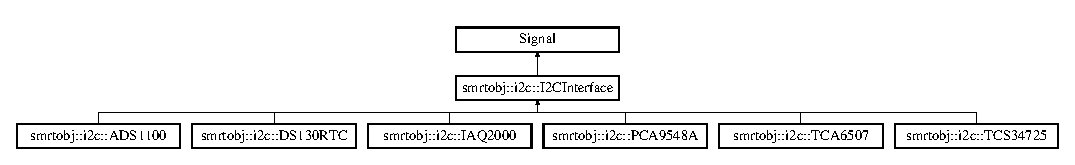
\includegraphics[height=1.772152cm]{classsmrtobj_1_1i2c_1_1_i2_c_interface}
\end{center}
\end{figure}
\subsection*{Public Member Functions}
\begin{DoxyCompactItemize}
\item 
\hyperlink{classsmrtobj_1_1i2c_1_1_i2_c_interface_ad28b942fde042a2231c02c961d50d486}{I2\+C\+Interface} ()
\item 
\hyperlink{classsmrtobj_1_1i2c_1_1_i2_c_interface_acad278c8a4b9c1794cdd1dce56fd93e4}{I2\+C\+Interface} (uint8\+\_\+t addr)
\item 
\hyperlink{classsmrtobj_1_1i2c_1_1_i2_c_interface_a9b21318916efb375e0af0bd475582667}{I2\+C\+Interface} (const \hyperlink{classsmrtobj_1_1i2c_1_1_i2_c_interface}{I2\+C\+Interface} \&d)
\item 
virtual \hyperlink{classsmrtobj_1_1i2c_1_1_i2_c_interface_a280499b65bc92b621239891132e47c2e}{$\sim$\+I2\+C\+Interface} ()
\item 
uint8\+\_\+t \hyperlink{classsmrtobj_1_1i2c_1_1_i2_c_interface_ab2130ffa3db4c06e503cfb4af06bb6ef}{address} ()
\item 
byte \hyperlink{classsmrtobj_1_1i2c_1_1_i2_c_interface_a87b9e2a2f654a34aaa37ded12d8a1501}{type} ()
\item 
\hyperlink{classsmrtobj_1_1i2c_1_1_i2_c_interface}{I2\+C\+Interface} \& \hyperlink{classsmrtobj_1_1i2c_1_1_i2_c_interface_a6187a562fce82125fd97c0b4643b9120}{operator=} (const \hyperlink{classsmrtobj_1_1i2c_1_1_i2_c_interface}{I2\+C\+Interface} \&d)
\item 
virtual bool \hyperlink{classsmrtobj_1_1i2c_1_1_i2_c_interface_a4ff1ff083d877c7c0816299b11965eb4}{initialize} ()=0
\item 
virtual bool \hyperlink{classsmrtobj_1_1i2c_1_1_i2_c_interface_a33fd37bafaf8c7e8184acb6470322bce}{is\+Connected} ()=0
\item 
virtual bool \hyperlink{classsmrtobj_1_1i2c_1_1_i2_c_interface_a58bc734662a60de6a7cb7976c2179753}{read} ()=0
\end{DoxyCompactItemize}
\subsection*{Protected Member Functions}
\begin{DoxyCompactItemize}
\item 
void \hyperlink{classsmrtobj_1_1i2c_1_1_i2_c_interface_aa4943f672d4cd56cfff8db8837c31824}{set\+Device\+Address} (uint8\+\_\+t addr)
\item 
bool \hyperlink{classsmrtobj_1_1i2c_1_1_i2_c_interface_a4692eedeaa640e42dbba829776b6646b}{read\+\_\+word} (uint16\+\_\+t \&value, bool M\+S\+B=true)
\item 
int8\+\_\+t \hyperlink{classsmrtobj_1_1i2c_1_1_i2_c_interface_acd7cd03741b455e1d48bb3e7da303bff}{read\+All\+Bytes} (uint8\+\_\+t dev\+Addr, uint8\+\_\+t length, uint8\+\_\+t $\ast$data, uint16\+\_\+t timeout=I2\+Cdev\+::read\+Timeout)
\item 
bool \hyperlink{classsmrtobj_1_1i2c_1_1_i2_c_interface_a64635dd37a944047ca793740ec1473f0}{write\+All\+Bytes} (uint8\+\_\+t dev\+Addr, uint8\+\_\+t length, uint8\+\_\+t $\ast$data, uint16\+\_\+t timeout=I2\+Cdev\+::read\+Timeout)
\end{DoxyCompactItemize}
\subsection*{Static Protected Member Functions}
\begin{DoxyCompactItemize}
\item 
static uint8\+\_\+t \hyperlink{classsmrtobj_1_1i2c_1_1_i2_c_interface_a56a637f360d7194e90fb1c7a6b5dd616}{dec2bcd} (uint8\+\_\+t num)
\item 
static uint8\+\_\+t \hyperlink{classsmrtobj_1_1i2c_1_1_i2_c_interface_a32d47650f01b2342e3f39639f643baf2}{bcd2dec} (uint8\+\_\+t num)
\end{DoxyCompactItemize}


\subsection{Detailed Description}
The \hyperlink{classsmrtobj_1_1i2c_1_1_i2_c_interface}{I2\+C\+Interface} class defines the standard interface of an I2\+C device sensor. An I2\+C device is identified by a address of one byte. This is a virtual class and defines four virtual method\+:
\begin{DoxyItemize}
\item initialize \+: initializes the device (if it is required by the datasheet specifics).
\item is\+Connected \+: verifies if the device is connected. It can be done trying to read a value from the device and testing if operation is successfully done.
\item read \+: read values from device
\item measure \+: calculate a measure or specific value from the all data read. 
\end{DoxyItemize}

Definition at line 37 of file i2cinterface.\+h.



\subsection{Constructor \& Destructor Documentation}
\hypertarget{classsmrtobj_1_1i2c_1_1_i2_c_interface_ad28b942fde042a2231c02c961d50d486}{}\index{smrtobj\+::i2c\+::\+I2\+C\+Interface@{smrtobj\+::i2c\+::\+I2\+C\+Interface}!I2\+C\+Interface@{I2\+C\+Interface}}
\index{I2\+C\+Interface@{I2\+C\+Interface}!smrtobj\+::i2c\+::\+I2\+C\+Interface@{smrtobj\+::i2c\+::\+I2\+C\+Interface}}
\subsubsection[{I2\+C\+Interface()}]{\setlength{\rightskip}{0pt plus 5cm}smrtobj\+::\+I2\+C\+Interface\+::\+I2\+C\+Interface (
\begin{DoxyParamCaption}
{}
\end{DoxyParamCaption}
)}\label{classsmrtobj_1_1i2c_1_1_i2_c_interface_ad28b942fde042a2231c02c961d50d486}
Default Constructor. Sets the default address to 0x00 and communication type as bidirectional (according to \hyperlink{classsmrtobj_1_1io_1_1_signal_a0566106724452894eae48ec38b66952c}{smrtobj\+::io\+::\+Signal\+::\+\_\+type} enum). 

Definition at line 13 of file i2cinterface.\+cpp.

\hypertarget{classsmrtobj_1_1i2c_1_1_i2_c_interface_acad278c8a4b9c1794cdd1dce56fd93e4}{}\index{smrtobj\+::i2c\+::\+I2\+C\+Interface@{smrtobj\+::i2c\+::\+I2\+C\+Interface}!I2\+C\+Interface@{I2\+C\+Interface}}
\index{I2\+C\+Interface@{I2\+C\+Interface}!smrtobj\+::i2c\+::\+I2\+C\+Interface@{smrtobj\+::i2c\+::\+I2\+C\+Interface}}
\subsubsection[{I2\+C\+Interface(uint8\+\_\+t addr)}]{\setlength{\rightskip}{0pt plus 5cm}smrtobj\+::\+I2\+C\+Interface\+::\+I2\+C\+Interface (
\begin{DoxyParamCaption}
\item[{uint8\+\_\+t}]{addr}
\end{DoxyParamCaption}
)}\label{classsmrtobj_1_1i2c_1_1_i2_c_interface_acad278c8a4b9c1794cdd1dce56fd93e4}
Constructor. Sets the device address and communication type as bidirectional (according to \hyperlink{classsmrtobj_1_1io_1_1_signal_a0566106724452894eae48ec38b66952c}{smrtobj\+::io\+::\+Signal\+::\+\_\+type} enum).


\begin{DoxyParams}[1]{Parameters}
\mbox{\tt in}  & {\em addr} & device address \\
\hline
\end{DoxyParams}


Definition at line 18 of file i2cinterface.\+cpp.

\hypertarget{classsmrtobj_1_1i2c_1_1_i2_c_interface_a9b21318916efb375e0af0bd475582667}{}\index{smrtobj\+::i2c\+::\+I2\+C\+Interface@{smrtobj\+::i2c\+::\+I2\+C\+Interface}!I2\+C\+Interface@{I2\+C\+Interface}}
\index{I2\+C\+Interface@{I2\+C\+Interface}!smrtobj\+::i2c\+::\+I2\+C\+Interface@{smrtobj\+::i2c\+::\+I2\+C\+Interface}}
\subsubsection[{I2\+C\+Interface(const I2\+C\+Interface \&d)}]{\setlength{\rightskip}{0pt plus 5cm}smrtobj\+::\+I2\+C\+Interface\+::\+I2\+C\+Interface (
\begin{DoxyParamCaption}
\item[{const {\bf I2\+C\+Interface} \&}]{d}
\end{DoxyParamCaption}
)}\label{classsmrtobj_1_1i2c_1_1_i2_c_interface_a9b21318916efb375e0af0bd475582667}
Copy Constructor.


\begin{DoxyParams}[1]{Parameters}
\mbox{\tt in}  & {\em d} & i2c device object \\
\hline
\end{DoxyParams}


Definition at line 23 of file i2cinterface.\+cpp.

\hypertarget{classsmrtobj_1_1i2c_1_1_i2_c_interface_a280499b65bc92b621239891132e47c2e}{}\index{smrtobj\+::i2c\+::\+I2\+C\+Interface@{smrtobj\+::i2c\+::\+I2\+C\+Interface}!````~I2\+C\+Interface@{$\sim$\+I2\+C\+Interface}}
\index{````~I2\+C\+Interface@{$\sim$\+I2\+C\+Interface}!smrtobj\+::i2c\+::\+I2\+C\+Interface@{smrtobj\+::i2c\+::\+I2\+C\+Interface}}
\subsubsection[{$\sim$\+I2\+C\+Interface()}]{\setlength{\rightskip}{0pt plus 5cm}smrtobj\+::\+I2\+C\+Interface\+::$\sim$\+I2\+C\+Interface (
\begin{DoxyParamCaption}
{}
\end{DoxyParamCaption}
)\hspace{0.3cm}{\ttfamily [virtual]}}\label{classsmrtobj_1_1i2c_1_1_i2_c_interface_a280499b65bc92b621239891132e47c2e}
Destructor. 

Definition at line 29 of file i2cinterface.\+cpp.



\subsection{Member Function Documentation}
\hypertarget{classsmrtobj_1_1i2c_1_1_i2_c_interface_ab2130ffa3db4c06e503cfb4af06bb6ef}{}\index{smrtobj\+::i2c\+::\+I2\+C\+Interface@{smrtobj\+::i2c\+::\+I2\+C\+Interface}!address@{address}}
\index{address@{address}!smrtobj\+::i2c\+::\+I2\+C\+Interface@{smrtobj\+::i2c\+::\+I2\+C\+Interface}}
\subsubsection[{address()}]{\setlength{\rightskip}{0pt plus 5cm}uint8\+\_\+t smrtobj\+::i2c\+::\+I2\+C\+Interface\+::address (
\begin{DoxyParamCaption}
{}
\end{DoxyParamCaption}
)\hspace{0.3cm}{\ttfamily [inline]}}\label{classsmrtobj_1_1i2c_1_1_i2_c_interface_ab2130ffa3db4c06e503cfb4af06bb6ef}
Returns the device address.

\begin{DoxyReturn}{Returns}
device address 
\end{DoxyReturn}


Definition at line 74 of file i2cinterface.\+h.

\hypertarget{classsmrtobj_1_1i2c_1_1_i2_c_interface_a32d47650f01b2342e3f39639f643baf2}{}\index{smrtobj\+::i2c\+::\+I2\+C\+Interface@{smrtobj\+::i2c\+::\+I2\+C\+Interface}!bcd2dec@{bcd2dec}}
\index{bcd2dec@{bcd2dec}!smrtobj\+::i2c\+::\+I2\+C\+Interface@{smrtobj\+::i2c\+::\+I2\+C\+Interface}}
\subsubsection[{bcd2dec(uint8\+\_\+t num)}]{\setlength{\rightskip}{0pt plus 5cm}uint8\+\_\+t smrtobj\+::\+I2\+C\+Interface\+::bcd2dec (
\begin{DoxyParamCaption}
\item[{uint8\+\_\+t}]{num}
\end{DoxyParamCaption}
)\hspace{0.3cm}{\ttfamily [static]}, {\ttfamily [protected]}}\label{classsmrtobj_1_1i2c_1_1_i2_c_interface_a32d47650f01b2342e3f39639f643baf2}
Converts a number (1 byte) from B\+C\+D to decimal


\begin{DoxyParams}[1]{Parameters}
\mbox{\tt in}  & {\em num} & B\+C\+D number\\
\hline
\end{DoxyParams}
\begin{DoxyReturn}{Returns}
B\+C\+D decimal 
\end{DoxyReturn}


Definition at line 138 of file i2cinterface.\+cpp.

\hypertarget{classsmrtobj_1_1i2c_1_1_i2_c_interface_a56a637f360d7194e90fb1c7a6b5dd616}{}\index{smrtobj\+::i2c\+::\+I2\+C\+Interface@{smrtobj\+::i2c\+::\+I2\+C\+Interface}!dec2bcd@{dec2bcd}}
\index{dec2bcd@{dec2bcd}!smrtobj\+::i2c\+::\+I2\+C\+Interface@{smrtobj\+::i2c\+::\+I2\+C\+Interface}}
\subsubsection[{dec2bcd(uint8\+\_\+t num)}]{\setlength{\rightskip}{0pt plus 5cm}uint8\+\_\+t smrtobj\+::\+I2\+C\+Interface\+::dec2bcd (
\begin{DoxyParamCaption}
\item[{uint8\+\_\+t}]{num}
\end{DoxyParamCaption}
)\hspace{0.3cm}{\ttfamily [static]}, {\ttfamily [protected]}}\label{classsmrtobj_1_1i2c_1_1_i2_c_interface_a56a637f360d7194e90fb1c7a6b5dd616}
Converts a number (1 byte) from decimal to B\+C\+D


\begin{DoxyParams}[1]{Parameters}
\mbox{\tt in}  & {\em num} & decimal number\\
\hline
\end{DoxyParams}
\begin{DoxyReturn}{Returns}
B\+C\+D number 
\end{DoxyReturn}


Definition at line 132 of file i2cinterface.\+cpp.

\hypertarget{classsmrtobj_1_1i2c_1_1_i2_c_interface_a4ff1ff083d877c7c0816299b11965eb4}{}\index{smrtobj\+::i2c\+::\+I2\+C\+Interface@{smrtobj\+::i2c\+::\+I2\+C\+Interface}!initialize@{initialize}}
\index{initialize@{initialize}!smrtobj\+::i2c\+::\+I2\+C\+Interface@{smrtobj\+::i2c\+::\+I2\+C\+Interface}}
\subsubsection[{initialize()=0}]{\setlength{\rightskip}{0pt plus 5cm}virtual bool smrtobj\+::i2c\+::\+I2\+C\+Interface\+::initialize (
\begin{DoxyParamCaption}
{}
\end{DoxyParamCaption}
)\hspace{0.3cm}{\ttfamily [pure virtual]}}\label{classsmrtobj_1_1i2c_1_1_i2_c_interface_a4ff1ff083d877c7c0816299b11965eb4}
Initializes the i2c device\+: power on and prepare for general usage. Virtual function, inheriting classes must define it.

\begin{DoxyReturn}{Returns}
true for success, or false if any error occurs. 
\end{DoxyReturn}


Implemented in \hyperlink{classsmrtobj_1_1i2c_1_1_t_c_a6507_a630cc83b260aceec29c3f26e2c4ebe5e}{smrtobj\+::i2c\+::\+T\+C\+A6507}, \hyperlink{classsmrtobj_1_1i2c_1_1_t_c_s34725_ace72ff801097ec771026acd605de2d53}{smrtobj\+::i2c\+::\+T\+C\+S34725}, \hyperlink{classsmrtobj_1_1i2c_1_1_p_c_a9548_a_aad4b31d15abdf2514592b045530d82f3}{smrtobj\+::i2c\+::\+P\+C\+A9548\+A}, \hyperlink{classsmrtobj_1_1i2c_1_1_d_s130_r_t_c_aef59c049dbca2d78877e607e8009452c}{smrtobj\+::i2c\+::\+D\+S130\+R\+T\+C}, \hyperlink{classsmrtobj_1_1i2c_1_1_a_d_s1100_af6a30ae17ea283aa979bbd933d84ee08}{smrtobj\+::i2c\+::\+A\+D\+S1100}, and \hyperlink{classsmrtobj_1_1i2c_1_1_i_a_q2000_ae586b35f7da1356a8acbe44e5e4911a1}{smrtobj\+::i2c\+::\+I\+A\+Q2000}.

\hypertarget{classsmrtobj_1_1i2c_1_1_i2_c_interface_a33fd37bafaf8c7e8184acb6470322bce}{}\index{smrtobj\+::i2c\+::\+I2\+C\+Interface@{smrtobj\+::i2c\+::\+I2\+C\+Interface}!is\+Connected@{is\+Connected}}
\index{is\+Connected@{is\+Connected}!smrtobj\+::i2c\+::\+I2\+C\+Interface@{smrtobj\+::i2c\+::\+I2\+C\+Interface}}
\subsubsection[{is\+Connected()=0}]{\setlength{\rightskip}{0pt plus 5cm}virtual bool smrtobj\+::i2c\+::\+I2\+C\+Interface\+::is\+Connected (
\begin{DoxyParamCaption}
{}
\end{DoxyParamCaption}
)\hspace{0.3cm}{\ttfamily [pure virtual]}}\label{classsmrtobj_1_1i2c_1_1_i2_c_interface_a33fd37bafaf8c7e8184acb6470322bce}
Tests if the device is connected. Make sure the device is connected and responds as expected. Virtual function, inheriting classes must define it.

\begin{DoxyReturn}{Returns}
true if connection is valid, false otherwise 
\end{DoxyReturn}


Implemented in \hyperlink{classsmrtobj_1_1i2c_1_1_t_c_a6507_aae2ceb7c2ba719a2d86d47f58cf16306}{smrtobj\+::i2c\+::\+T\+C\+A6507}, \hyperlink{classsmrtobj_1_1i2c_1_1_t_c_s34725_af9018c2f326e228d998866692393090f}{smrtobj\+::i2c\+::\+T\+C\+S34725}, \hyperlink{classsmrtobj_1_1i2c_1_1_p_c_a9548_a_a2a697b995f40560498d2721a1e99e94a}{smrtobj\+::i2c\+::\+P\+C\+A9548\+A}, \hyperlink{classsmrtobj_1_1i2c_1_1_d_s130_r_t_c_ad8630568cd75431db924e2e723ebfcb4}{smrtobj\+::i2c\+::\+D\+S130\+R\+T\+C}, \hyperlink{classsmrtobj_1_1i2c_1_1_a_d_s1100_a707ea27963bcca7465d51195cee0af04}{smrtobj\+::i2c\+::\+A\+D\+S1100}, and \hyperlink{classsmrtobj_1_1i2c_1_1_i_a_q2000_a3efac4a4e37fd0d061e69ba185df3100}{smrtobj\+::i2c\+::\+I\+A\+Q2000}.

\hypertarget{classsmrtobj_1_1i2c_1_1_i2_c_interface_a6187a562fce82125fd97c0b4643b9120}{}\index{smrtobj\+::i2c\+::\+I2\+C\+Interface@{smrtobj\+::i2c\+::\+I2\+C\+Interface}!operator=@{operator=}}
\index{operator=@{operator=}!smrtobj\+::i2c\+::\+I2\+C\+Interface@{smrtobj\+::i2c\+::\+I2\+C\+Interface}}
\subsubsection[{operator=(const I2\+C\+Interface \&d)}]{\setlength{\rightskip}{0pt plus 5cm}{\bf I2\+C\+Interface} \& smrtobj\+::\+I2\+C\+Interface\+::operator= (
\begin{DoxyParamCaption}
\item[{const {\bf I2\+C\+Interface} \&}]{d}
\end{DoxyParamCaption}
)}\label{classsmrtobj_1_1i2c_1_1_i2_c_interface_a6187a562fce82125fd97c0b4643b9120}
Override operator =


\begin{DoxyParams}[1]{Parameters}
\mbox{\tt in}  & {\em d} & source device object\\
\hline
\end{DoxyParams}
\begin{DoxyReturn}{Returns}
destination signal reference 
\end{DoxyReturn}


Definition at line 33 of file i2cinterface.\+cpp.

\hypertarget{classsmrtobj_1_1i2c_1_1_i2_c_interface_a58bc734662a60de6a7cb7976c2179753}{}\index{smrtobj\+::i2c\+::\+I2\+C\+Interface@{smrtobj\+::i2c\+::\+I2\+C\+Interface}!read@{read}}
\index{read@{read}!smrtobj\+::i2c\+::\+I2\+C\+Interface@{smrtobj\+::i2c\+::\+I2\+C\+Interface}}
\subsubsection[{read()=0}]{\setlength{\rightskip}{0pt plus 5cm}virtual bool smrtobj\+::i2c\+::\+I2\+C\+Interface\+::read (
\begin{DoxyParamCaption}
{}
\end{DoxyParamCaption}
)\hspace{0.3cm}{\ttfamily [pure virtual]}}\label{classsmrtobj_1_1i2c_1_1_i2_c_interface_a58bc734662a60de6a7cb7976c2179753}
Reads data from the i2c device.

\begin{DoxyReturn}{Returns}
true if connection is valid, false otherwise 
\end{DoxyReturn}


Implemented in \hyperlink{classsmrtobj_1_1i2c_1_1_t_c_a6507_adce687bb4bd2f248a1851b5d3e290181}{smrtobj\+::i2c\+::\+T\+C\+A6507}, \hyperlink{classsmrtobj_1_1i2c_1_1_t_c_s34725_ae00be04f529c449287ac9329df3cb7a7}{smrtobj\+::i2c\+::\+T\+C\+S34725}, \hyperlink{classsmrtobj_1_1i2c_1_1_p_c_a9548_a_af1dceb4c9b1cd4d4a1b15888ec793d38}{smrtobj\+::i2c\+::\+P\+C\+A9548\+A}, \hyperlink{classsmrtobj_1_1i2c_1_1_d_s130_r_t_c_afc3af98fb550808741d738655ce642d1}{smrtobj\+::i2c\+::\+D\+S130\+R\+T\+C}, \hyperlink{classsmrtobj_1_1i2c_1_1_a_d_s1100_ae57857e0b925c23af5406773bbaa3da9}{smrtobj\+::i2c\+::\+A\+D\+S1100}, and \hyperlink{classsmrtobj_1_1i2c_1_1_i_a_q2000_a026848c4fca394f36929c7d831a675aa}{smrtobj\+::i2c\+::\+I\+A\+Q2000}.

\hypertarget{classsmrtobj_1_1i2c_1_1_i2_c_interface_a4692eedeaa640e42dbba829776b6646b}{}\index{smrtobj\+::i2c\+::\+I2\+C\+Interface@{smrtobj\+::i2c\+::\+I2\+C\+Interface}!read\+\_\+word@{read\+\_\+word}}
\index{read\+\_\+word@{read\+\_\+word}!smrtobj\+::i2c\+::\+I2\+C\+Interface@{smrtobj\+::i2c\+::\+I2\+C\+Interface}}
\subsubsection[{read\+\_\+word(uint16\+\_\+t \&value, bool M\+S\+B=true)}]{\setlength{\rightskip}{0pt plus 5cm}bool smrtobj\+::\+I2\+C\+Interface\+::read\+\_\+word (
\begin{DoxyParamCaption}
\item[{uint16\+\_\+t \&}]{value, }
\item[{bool}]{M\+S\+B = {\ttfamily true}}
\end{DoxyParamCaption}
)\hspace{0.3cm}{\ttfamily [protected]}}\label{classsmrtobj_1_1i2c_1_1_i2_c_interface_a4692eedeaa640e42dbba829776b6646b}
Reads a word (2 byte) from i2c device.


\begin{DoxyParams}[1]{Parameters}
\mbox{\tt out}  & {\em value} & data read \\
\hline
\mbox{\tt in}  & {\em M\+S\+B} & true if data is in format Most Significant Byte, false if it is Less Significat Byte\\
\hline
\end{DoxyParams}
\begin{DoxyReturn}{Returns}
false in case of errors, true otherwise 
\end{DoxyReturn}


Definition at line 119 of file i2cinterface.\+cpp.

\hypertarget{classsmrtobj_1_1i2c_1_1_i2_c_interface_acd7cd03741b455e1d48bb3e7da303bff}{}\index{smrtobj\+::i2c\+::\+I2\+C\+Interface@{smrtobj\+::i2c\+::\+I2\+C\+Interface}!read\+All\+Bytes@{read\+All\+Bytes}}
\index{read\+All\+Bytes@{read\+All\+Bytes}!smrtobj\+::i2c\+::\+I2\+C\+Interface@{smrtobj\+::i2c\+::\+I2\+C\+Interface}}
\subsubsection[{read\+All\+Bytes(uint8\+\_\+t dev\+Addr, uint8\+\_\+t length, uint8\+\_\+t $\ast$data, uint16\+\_\+t timeout=\+I2\+Cdev\+::read\+Timeout)}]{\setlength{\rightskip}{0pt plus 5cm}int8\+\_\+t smrtobj\+::\+I2\+C\+Interface\+::read\+All\+Bytes (
\begin{DoxyParamCaption}
\item[{uint8\+\_\+t}]{dev\+Addr, }
\item[{uint8\+\_\+t}]{length, }
\item[{uint8\+\_\+t $\ast$}]{data, }
\item[{uint16\+\_\+t}]{timeout = {\ttfamily I2Cdev\+:\+:readTimeout}}
\end{DoxyParamCaption}
)\hspace{0.3cm}{\ttfamily [protected]}}\label{classsmrtobj_1_1i2c_1_1_i2_c_interface_acd7cd03741b455e1d48bb3e7da303bff}
Reads bytes from a slave device. This is a \char`\"{}stripped-\/down\char`\"{} version of the standard Jeff Rowberg\textquotesingle{}s I2\+Cdev\+::read\+Bytes method, which apparently does not support setting of an address pointer to indicate from which position is to start read from.


\begin{DoxyParams}[1]{Parameters}
\mbox{\tt in}  & {\em dev\+Addr} & Address of the slave device to read bytes from \\
\hline
\mbox{\tt in}  & {\em length} & Number of bytes to read \\
\hline
\mbox{\tt out}  & {\em data} & Buffer to store read data in \\
\hline
\mbox{\tt in}  & {\em timeout} & Optional read timeout in milliseconds (0 to disable, leave off to use default class value in I2\+Cdev\+::read\+Timeout)\\
\hline
\end{DoxyParams}
\begin{DoxyReturn}{Returns}
Number of bytes read (0 indicates failure) 
\end{DoxyReturn}


Definition at line 43 of file i2cinterface.\+cpp.

\hypertarget{classsmrtobj_1_1i2c_1_1_i2_c_interface_aa4943f672d4cd56cfff8db8837c31824}{}\index{smrtobj\+::i2c\+::\+I2\+C\+Interface@{smrtobj\+::i2c\+::\+I2\+C\+Interface}!set\+Device\+Address@{set\+Device\+Address}}
\index{set\+Device\+Address@{set\+Device\+Address}!smrtobj\+::i2c\+::\+I2\+C\+Interface@{smrtobj\+::i2c\+::\+I2\+C\+Interface}}
\subsubsection[{set\+Device\+Address(uint8\+\_\+t addr)}]{\setlength{\rightskip}{0pt plus 5cm}void smrtobj\+::i2c\+::\+I2\+C\+Interface\+::set\+Device\+Address (
\begin{DoxyParamCaption}
\item[{uint8\+\_\+t}]{addr}
\end{DoxyParamCaption}
)\hspace{0.3cm}{\ttfamily [inline]}, {\ttfamily [protected]}}\label{classsmrtobj_1_1i2c_1_1_i2_c_interface_aa4943f672d4cd56cfff8db8837c31824}
Sets the device address. This function must be called only by constructors.


\begin{DoxyParams}[1]{Parameters}
\mbox{\tt in}  & {\em addr} & device address \\
\hline
\end{DoxyParams}


Definition at line 140 of file i2cinterface.\+h.

\hypertarget{classsmrtobj_1_1i2c_1_1_i2_c_interface_a87b9e2a2f654a34aaa37ded12d8a1501}{}\index{smrtobj\+::i2c\+::\+I2\+C\+Interface@{smrtobj\+::i2c\+::\+I2\+C\+Interface}!type@{type}}
\index{type@{type}!smrtobj\+::i2c\+::\+I2\+C\+Interface@{smrtobj\+::i2c\+::\+I2\+C\+Interface}}
\subsubsection[{type()}]{\setlength{\rightskip}{0pt plus 5cm}byte smrtobj\+::i2c\+::\+I2\+C\+Interface\+::type (
\begin{DoxyParamCaption}
{}
\end{DoxyParamCaption}
)\hspace{0.3cm}{\ttfamily [inline]}}\label{classsmrtobj_1_1i2c_1_1_i2_c_interface_a87b9e2a2f654a34aaa37ded12d8a1501}
Gets the type of the interface according to \hyperlink{classsmrtobj_1_1io_1_1_signal_a0566106724452894eae48ec38b66952c}{smrtobj\+::io\+::\+Signal\+::\+\_\+type} enum

\begin{DoxyReturn}{Returns}
type of the interface 
\end{DoxyReturn}


Definition at line 81 of file i2cinterface.\+h.

\hypertarget{classsmrtobj_1_1i2c_1_1_i2_c_interface_a64635dd37a944047ca793740ec1473f0}{}\index{smrtobj\+::i2c\+::\+I2\+C\+Interface@{smrtobj\+::i2c\+::\+I2\+C\+Interface}!write\+All\+Bytes@{write\+All\+Bytes}}
\index{write\+All\+Bytes@{write\+All\+Bytes}!smrtobj\+::i2c\+::\+I2\+C\+Interface@{smrtobj\+::i2c\+::\+I2\+C\+Interface}}
\subsubsection[{write\+All\+Bytes(uint8\+\_\+t dev\+Addr, uint8\+\_\+t length, uint8\+\_\+t $\ast$data, uint16\+\_\+t timeout=\+I2\+Cdev\+::read\+Timeout)}]{\setlength{\rightskip}{0pt plus 5cm}bool smrtobj\+::\+I2\+C\+Interface\+::write\+All\+Bytes (
\begin{DoxyParamCaption}
\item[{uint8\+\_\+t}]{dev\+Addr, }
\item[{uint8\+\_\+t}]{length, }
\item[{uint8\+\_\+t $\ast$}]{data, }
\item[{uint16\+\_\+t}]{timeout = {\ttfamily I2Cdev\+:\+:readTimeout}}
\end{DoxyParamCaption}
)\hspace{0.3cm}{\ttfamily [protected]}}\label{classsmrtobj_1_1i2c_1_1_i2_c_interface_a64635dd37a944047ca793740ec1473f0}
Writes bytes to a slave device. This is a \char`\"{}stripped-\/down\char`\"{} version of the standard Jeff Rowberg\textquotesingle{}s I2\+Cdev\+::write\+Bytes method, which apparently does not support setting of an address pointer to indicate from which position is to start read from.


\begin{DoxyParams}[1]{Parameters}
\mbox{\tt in}  & {\em dev\+Addr} & Address of the slave device to write bytes to \\
\hline
\mbox{\tt in}  & {\em length} & Number of bytes to write \\
\hline
\mbox{\tt in}  & {\em data} & Buffer with data to write \\
\hline
\mbox{\tt in}  & {\em timeout} & Optional read timeout in milliseconds (0 to disable, leave off to use default class value in I2\+Cdev\+::read\+Timeout)\\
\hline
\end{DoxyParams}
\begin{DoxyReturn}{Returns}
false in case of errors, true otherwise 
\end{DoxyReturn}


Definition at line 79 of file i2cinterface.\+cpp.



The documentation for this class was generated from the following files\+:\begin{DoxyCompactItemize}
\item 
libraries/\+Smrt\+Obj\+I2\+C/src/interfaces/\hyperlink{i2cinterface_8h}{i2cinterface.\+h}\item 
libraries/\+Smrt\+Obj\+I2\+C/src/interfaces/\hyperlink{i2cinterface_8cpp}{i2cinterface.\+cpp}\end{DoxyCompactItemize}

\hypertarget{classsmrtobj_1_1i2c_1_1_i_a_q2000}{}\section{smrtobj\+:\+:i2c\+:\+:I\+A\+Q2000 Class Reference}
\label{classsmrtobj_1_1i2c_1_1_i_a_q2000}\index{smrtobj\+::i2c\+::\+I\+A\+Q2000@{smrtobj\+::i2c\+::\+I\+A\+Q2000}}


{\ttfamily \#include $<$I\+A\+Q2000.\+h$>$}

Inheritance diagram for smrtobj\+:\+:i2c\+:\+:I\+A\+Q2000\+:\begin{figure}[H]
\begin{center}
\leavevmode
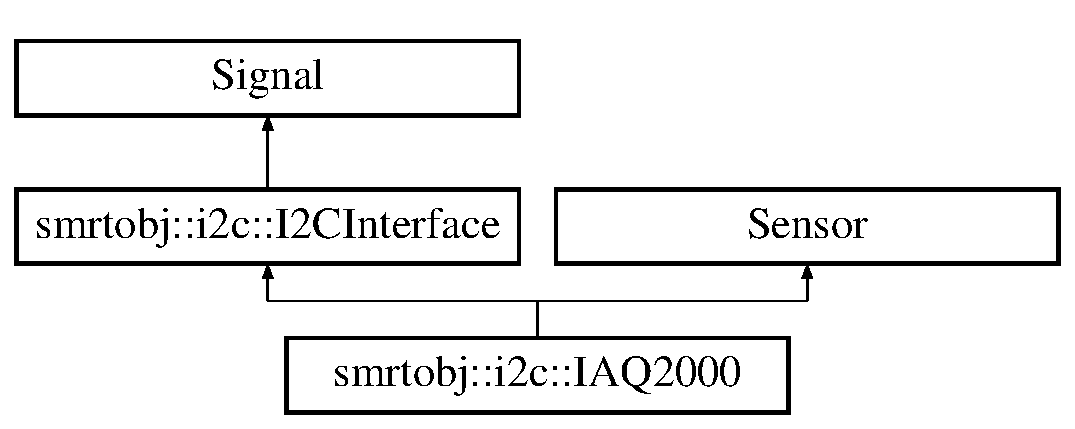
\includegraphics[height=3.000000cm]{classsmrtobj_1_1i2c_1_1_i_a_q2000}
\end{center}
\end{figure}
\subsection*{Public Member Functions}
\begin{DoxyCompactItemize}
\item 
\hyperlink{classsmrtobj_1_1i2c_1_1_i_a_q2000_a4261abb895def12fc22dcc528936d761}{I\+A\+Q2000} ()
\item 
\hyperlink{classsmrtobj_1_1i2c_1_1_i_a_q2000_a3562f73c2c8403fb86b8647051e22842}{I\+A\+Q2000} (const \hyperlink{classsmrtobj_1_1i2c_1_1_i_a_q2000}{I\+A\+Q2000} \&s)
\item 
virtual \hyperlink{classsmrtobj_1_1i2c_1_1_i_a_q2000_aa2cb430098fc621f69de12d74a1fc39f}{$\sim$\+I\+A\+Q2000} ()
\item 
\hyperlink{classsmrtobj_1_1i2c_1_1_i_a_q2000}{I\+A\+Q2000} \& \hyperlink{classsmrtobj_1_1i2c_1_1_i_a_q2000_a79a72c585448c25db99a0af5e8f660af}{operator=} (const \hyperlink{classsmrtobj_1_1i2c_1_1_i_a_q2000}{I\+A\+Q2000} \&s)
\item 
virtual bool \hyperlink{classsmrtobj_1_1i2c_1_1_i_a_q2000_ae586b35f7da1356a8acbe44e5e4911a1}{initialize} ()
\item 
virtual bool \hyperlink{classsmrtobj_1_1i2c_1_1_i_a_q2000_a3efac4a4e37fd0d061e69ba185df3100}{is\+Connected} ()
\item 
virtual bool \hyperlink{classsmrtobj_1_1i2c_1_1_i_a_q2000_a026848c4fca394f36929c7d831a675aa}{read} ()
\item 
virtual float \hyperlink{classsmrtobj_1_1i2c_1_1_i_a_q2000_ad1b66960d4ec931dd3535f7b220a2251}{measure} ()
\item 
uint16\+\_\+t \hyperlink{classsmrtobj_1_1i2c_1_1_i_a_q2000_ad08f070b9bb2ad32f3b16b69b44eb4f8}{value} ()
\end{DoxyCompactItemize}
\subsection*{Static Public Attributes}
\begin{DoxyCompactItemize}
\item 
\hypertarget{classsmrtobj_1_1i2c_1_1_i_a_q2000_a7497e793ec38667bcc8722fe833fbe74}{}static const uint8\+\_\+t \hyperlink{classsmrtobj_1_1i2c_1_1_i_a_q2000_a7497e793ec38667bcc8722fe833fbe74}{D\+E\+V\+I\+C\+E\+\_\+\+A\+D\+D\+R\+E\+S\+S} = 0x5\+A\label{classsmrtobj_1_1i2c_1_1_i_a_q2000_a7497e793ec38667bcc8722fe833fbe74}

\begin{DoxyCompactList}\small\item\em Device address used by default. \end{DoxyCompactList}\end{DoxyCompactItemize}
\subsection*{Additional Inherited Members}


\subsection{Detailed Description}
Class \hyperlink{classsmrtobj_1_1i2c_1_1_i_a_q2000}{I\+A\+Q2000} models the I2\+C i\+A\+Q2000 sensor. The i\+A\+Q2000 is designed to sense the level of volatile organic compounds (V\+O\+Cs) such as smoke, cooking odors, bio-\/effluence and pollutants. This sensor gives a direct and reliable correlation to C\+O2 levels\+: output in ppm (parts-\/per-\/million)\+: predicted C\+O2 concentration based on human induced volatile organic compounds (V\+O\+C) detection (in ppm V\+O\+C + C\+O2 equivalents) 

Definition at line 29 of file I\+A\+Q2000.\+h.



\subsection{Constructor \& Destructor Documentation}
\hypertarget{classsmrtobj_1_1i2c_1_1_i_a_q2000_a4261abb895def12fc22dcc528936d761}{}\index{smrtobj\+::i2c\+::\+I\+A\+Q2000@{smrtobj\+::i2c\+::\+I\+A\+Q2000}!I\+A\+Q2000@{I\+A\+Q2000}}
\index{I\+A\+Q2000@{I\+A\+Q2000}!smrtobj\+::i2c\+::\+I\+A\+Q2000@{smrtobj\+::i2c\+::\+I\+A\+Q2000}}
\subsubsection[{I\+A\+Q2000()}]{\setlength{\rightskip}{0pt plus 5cm}smrtobj\+::i2c\+::\+I\+A\+Q2000\+::\+I\+A\+Q2000 (
\begin{DoxyParamCaption}
{}
\end{DoxyParamCaption}
)}\label{classsmrtobj_1_1i2c_1_1_i_a_q2000_a4261abb895def12fc22dcc528936d761}
Default Constructor. Sets the device address. 

Definition at line 22 of file I\+A\+Q2000.\+cpp.

\hypertarget{classsmrtobj_1_1i2c_1_1_i_a_q2000_a3562f73c2c8403fb86b8647051e22842}{}\index{smrtobj\+::i2c\+::\+I\+A\+Q2000@{smrtobj\+::i2c\+::\+I\+A\+Q2000}!I\+A\+Q2000@{I\+A\+Q2000}}
\index{I\+A\+Q2000@{I\+A\+Q2000}!smrtobj\+::i2c\+::\+I\+A\+Q2000@{smrtobj\+::i2c\+::\+I\+A\+Q2000}}
\subsubsection[{I\+A\+Q2000(const I\+A\+Q2000 \&s)}]{\setlength{\rightskip}{0pt plus 5cm}smrtobj\+::i2c\+::\+I\+A\+Q2000\+::\+I\+A\+Q2000 (
\begin{DoxyParamCaption}
\item[{const {\bf I\+A\+Q2000} \&}]{s}
\end{DoxyParamCaption}
)}\label{classsmrtobj_1_1i2c_1_1_i_a_q2000_a3562f73c2c8403fb86b8647051e22842}
Copy Constructor.


\begin{DoxyParams}[1]{Parameters}
\mbox{\tt in}  & {\em s} & i2c sensor object \\
\hline
\end{DoxyParams}


Definition at line 27 of file I\+A\+Q2000.\+cpp.

\hypertarget{classsmrtobj_1_1i2c_1_1_i_a_q2000_aa2cb430098fc621f69de12d74a1fc39f}{}\index{smrtobj\+::i2c\+::\+I\+A\+Q2000@{smrtobj\+::i2c\+::\+I\+A\+Q2000}!````~I\+A\+Q2000@{$\sim$\+I\+A\+Q2000}}
\index{````~I\+A\+Q2000@{$\sim$\+I\+A\+Q2000}!smrtobj\+::i2c\+::\+I\+A\+Q2000@{smrtobj\+::i2c\+::\+I\+A\+Q2000}}
\subsubsection[{$\sim$\+I\+A\+Q2000()}]{\setlength{\rightskip}{0pt plus 5cm}smrtobj\+::i2c\+::\+I\+A\+Q2000\+::$\sim$\+I\+A\+Q2000 (
\begin{DoxyParamCaption}
{}
\end{DoxyParamCaption}
)\hspace{0.3cm}{\ttfamily [virtual]}}\label{classsmrtobj_1_1i2c_1_1_i_a_q2000_aa2cb430098fc621f69de12d74a1fc39f}
Destructor. 

Definition at line 32 of file I\+A\+Q2000.\+cpp.



\subsection{Member Function Documentation}
\hypertarget{classsmrtobj_1_1i2c_1_1_i_a_q2000_ae586b35f7da1356a8acbe44e5e4911a1}{}\index{smrtobj\+::i2c\+::\+I\+A\+Q2000@{smrtobj\+::i2c\+::\+I\+A\+Q2000}!initialize@{initialize}}
\index{initialize@{initialize}!smrtobj\+::i2c\+::\+I\+A\+Q2000@{smrtobj\+::i2c\+::\+I\+A\+Q2000}}
\subsubsection[{initialize()}]{\setlength{\rightskip}{0pt plus 5cm}bool smrtobj\+::i2c\+::\+I\+A\+Q2000\+::initialize (
\begin{DoxyParamCaption}
{}
\end{DoxyParamCaption}
)\hspace{0.3cm}{\ttfamily [virtual]}}\label{classsmrtobj_1_1i2c_1_1_i_a_q2000_ae586b35f7da1356a8acbe44e5e4911a1}
Initializes the i2c device\+: power on and prepare for general usage. Nothing is required by this device.

\begin{DoxyReturn}{Returns}
true for success, or false if any error occurs. 
\end{DoxyReturn}


Implements \hyperlink{classsmrtobj_1_1i2c_1_1_i2_c_interface_a4ff1ff083d877c7c0816299b11965eb4}{smrtobj\+::i2c\+::\+I2\+C\+Interface}.



Definition at line 46 of file I\+A\+Q2000.\+cpp.

\hypertarget{classsmrtobj_1_1i2c_1_1_i_a_q2000_a3efac4a4e37fd0d061e69ba185df3100}{}\index{smrtobj\+::i2c\+::\+I\+A\+Q2000@{smrtobj\+::i2c\+::\+I\+A\+Q2000}!is\+Connected@{is\+Connected}}
\index{is\+Connected@{is\+Connected}!smrtobj\+::i2c\+::\+I\+A\+Q2000@{smrtobj\+::i2c\+::\+I\+A\+Q2000}}
\subsubsection[{is\+Connected()}]{\setlength{\rightskip}{0pt plus 5cm}bool smrtobj\+::i2c\+::\+I\+A\+Q2000\+::is\+Connected (
\begin{DoxyParamCaption}
{}
\end{DoxyParamCaption}
)\hspace{0.3cm}{\ttfamily [virtual]}}\label{classsmrtobj_1_1i2c_1_1_i_a_q2000_a3efac4a4e37fd0d061e69ba185df3100}
Tests if the device is connected. Make sure the device is connected and responds as expected.

\begin{DoxyReturn}{Returns}
true if connection is valid, false otherwise 
\end{DoxyReturn}


Implements \hyperlink{classsmrtobj_1_1i2c_1_1_i2_c_interface_a33fd37bafaf8c7e8184acb6470322bce}{smrtobj\+::i2c\+::\+I2\+C\+Interface}.



Definition at line 52 of file I\+A\+Q2000.\+cpp.

\hypertarget{classsmrtobj_1_1i2c_1_1_i_a_q2000_ad1b66960d4ec931dd3535f7b220a2251}{}\index{smrtobj\+::i2c\+::\+I\+A\+Q2000@{smrtobj\+::i2c\+::\+I\+A\+Q2000}!measure@{measure}}
\index{measure@{measure}!smrtobj\+::i2c\+::\+I\+A\+Q2000@{smrtobj\+::i2c\+::\+I\+A\+Q2000}}
\subsubsection[{measure()}]{\setlength{\rightskip}{0pt plus 5cm}float smrtobj\+::i2c\+::\+I\+A\+Q2000\+::measure (
\begin{DoxyParamCaption}
{}
\end{DoxyParamCaption}
)\hspace{0.3cm}{\ttfamily [virtual]}}\label{classsmrtobj_1_1i2c_1_1_i_a_q2000_ad1b66960d4ec931dd3535f7b220a2251}
Returns last data read as a floating point number.

\begin{DoxyReturn}{Returns}
last data read 
\end{DoxyReturn}


Definition at line 68 of file I\+A\+Q2000.\+cpp.

\hypertarget{classsmrtobj_1_1i2c_1_1_i_a_q2000_a79a72c585448c25db99a0af5e8f660af}{}\index{smrtobj\+::i2c\+::\+I\+A\+Q2000@{smrtobj\+::i2c\+::\+I\+A\+Q2000}!operator=@{operator=}}
\index{operator=@{operator=}!smrtobj\+::i2c\+::\+I\+A\+Q2000@{smrtobj\+::i2c\+::\+I\+A\+Q2000}}
\subsubsection[{operator=(const I\+A\+Q2000 \&s)}]{\setlength{\rightskip}{0pt plus 5cm}{\bf I\+A\+Q2000} \& smrtobj\+::i2c\+::\+I\+A\+Q2000\+::operator= (
\begin{DoxyParamCaption}
\item[{const {\bf I\+A\+Q2000} \&}]{s}
\end{DoxyParamCaption}
)}\label{classsmrtobj_1_1i2c_1_1_i_a_q2000_a79a72c585448c25db99a0af5e8f660af}
Override operator =


\begin{DoxyParams}[1]{Parameters}
\mbox{\tt in}  & {\em s} & source signal object\\
\hline
\end{DoxyParams}
\begin{DoxyReturn}{Returns}
destination signal reference 
\end{DoxyReturn}


Definition at line 36 of file I\+A\+Q2000.\+cpp.

\hypertarget{classsmrtobj_1_1i2c_1_1_i_a_q2000_a026848c4fca394f36929c7d831a675aa}{}\index{smrtobj\+::i2c\+::\+I\+A\+Q2000@{smrtobj\+::i2c\+::\+I\+A\+Q2000}!read@{read}}
\index{read@{read}!smrtobj\+::i2c\+::\+I\+A\+Q2000@{smrtobj\+::i2c\+::\+I\+A\+Q2000}}
\subsubsection[{read()}]{\setlength{\rightskip}{0pt plus 5cm}bool smrtobj\+::i2c\+::\+I\+A\+Q2000\+::read (
\begin{DoxyParamCaption}
{}
\end{DoxyParamCaption}
)\hspace{0.3cm}{\ttfamily [virtual]}}\label{classsmrtobj_1_1i2c_1_1_i_a_q2000_a026848c4fca394f36929c7d831a675aa}
Reads data from the i2c device. This function read 2 byte\+:
\begin{DoxyItemize}
\item 1st byte (Byte0) is the most significant byte
\item 2nd byte (Byte1) is the less significant byte Data is calculate as\+: value = (Byte0\mbox{]} $<$$<$ 8) $\vert$ Byte1; The value read is stored in m\+\_\+value.
\end{DoxyItemize}

\begin{DoxyReturn}{Returns}
true for success, or false if any error occurs. 
\end{DoxyReturn}


Implements \hyperlink{classsmrtobj_1_1i2c_1_1_i2_c_interface_a58bc734662a60de6a7cb7976c2179753}{smrtobj\+::i2c\+::\+I2\+C\+Interface}.



Definition at line 64 of file I\+A\+Q2000.\+cpp.

\hypertarget{classsmrtobj_1_1i2c_1_1_i_a_q2000_ad08f070b9bb2ad32f3b16b69b44eb4f8}{}\index{smrtobj\+::i2c\+::\+I\+A\+Q2000@{smrtobj\+::i2c\+::\+I\+A\+Q2000}!value@{value}}
\index{value@{value}!smrtobj\+::i2c\+::\+I\+A\+Q2000@{smrtobj\+::i2c\+::\+I\+A\+Q2000}}
\subsubsection[{value()}]{\setlength{\rightskip}{0pt plus 5cm}uint16\+\_\+t smrtobj\+::i2c\+::\+I\+A\+Q2000\+::value (
\begin{DoxyParamCaption}
{}
\end{DoxyParamCaption}
)\hspace{0.3cm}{\ttfamily [inline]}}\label{classsmrtobj_1_1i2c_1_1_i_a_q2000_ad08f070b9bb2ad32f3b16b69b44eb4f8}
Returns last value read as unsigned integer of 16 bits.

\begin{DoxyReturn}{Returns}
last value read 
\end{DoxyReturn}


Definition at line 103 of file I\+A\+Q2000.\+h.



The documentation for this class was generated from the following files\+:\begin{DoxyCompactItemize}
\item 
libraries/\+Smrt\+Obj\+I2\+C/src/sensors/\hyperlink{_i_a_q2000_8h}{I\+A\+Q2000.\+h}\item 
libraries/\+Smrt\+Obj\+I2\+C/src/sensors/\hyperlink{_i_a_q2000_8cpp}{I\+A\+Q2000.\+cpp}\end{DoxyCompactItemize}

\hypertarget{classsmrtobj_1_1timer_1_1_interval}{}\section{smrtobj\+:\+:timer\+:\+:Interval Class Reference}
\label{classsmrtobj_1_1timer_1_1_interval}\index{smrtobj\+::timer\+::\+Interval@{smrtobj\+::timer\+::\+Interval}}


{\ttfamily \#include $<$interval.\+h$>$}

Inheritance diagram for smrtobj\+:\+:timer\+:\+:Interval\+:\begin{figure}[H]
\begin{center}
\leavevmode
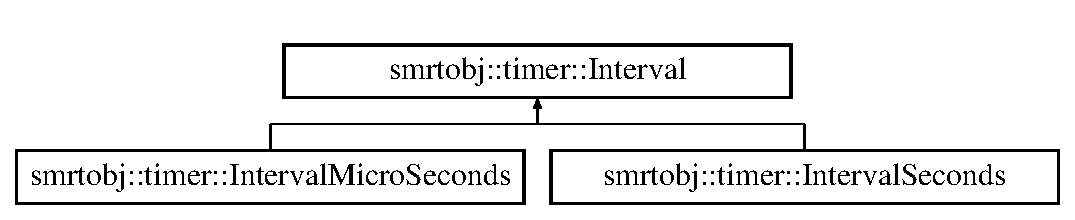
\includegraphics[height=2.000000cm]{classsmrtobj_1_1timer_1_1_interval}
\end{center}
\end{figure}
\subsection*{Public Member Functions}
\begin{DoxyCompactItemize}
\item 
\hyperlink{classsmrtobj_1_1timer_1_1_interval_aaf7a279101cc8d105693107d9bdcb26a}{Interval} ()
\item 
\hyperlink{classsmrtobj_1_1timer_1_1_interval_a1b2142dfa79eb5535a88609045a24d6e}{Interval} (unsigned long \hyperlink{classsmrtobj_1_1timer_1_1_interval_a323a909c95c592217e9be9cd5a313cb9}{start})
\item 
\hyperlink{classsmrtobj_1_1timer_1_1_interval_a7f90e3bf2de5acf32809e0c2379f2228}{Interval} (const \hyperlink{classsmrtobj_1_1timer_1_1_interval}{Interval} \&s)
\item 
virtual \hyperlink{classsmrtobj_1_1timer_1_1_interval_a3425f23d684c0c7501400f4dcc199078}{$\sim$\+Interval} ()
\item 
void \hyperlink{classsmrtobj_1_1timer_1_1_interval_a410562823bb9c16de498db2fbe2b14ec}{update} ()
\item 
unsigned long \hyperlink{classsmrtobj_1_1timer_1_1_interval_a323a909c95c592217e9be9cd5a313cb9}{start} ()
\item 
void \hyperlink{classsmrtobj_1_1timer_1_1_interval_aff1a426750f4c2f5534387ed2e8a8bdc}{reset} (unsigned long \hyperlink{classsmrtobj_1_1timer_1_1_interval_a323a909c95c592217e9be9cd5a313cb9}{start}=0)
\item 
unsigned long \hyperlink{classsmrtobj_1_1timer_1_1_interval_ae94300e5c29ba819eaaeb343b7caaeb5}{time} ()
\item 
unsigned long \hyperlink{classsmrtobj_1_1timer_1_1_interval_a1a3cef1ea187fad7f4abd1ee51dba09a}{residual\+Time} (unsigned long end\+Time)
\item 
\hyperlink{classsmrtobj_1_1timer_1_1_interval}{Interval} \& \hyperlink{classsmrtobj_1_1timer_1_1_interval_a3436785777d0868204112c72d5d2cace}{operator=} (const \hyperlink{classsmrtobj_1_1timer_1_1_interval}{Interval} \&)
\end{DoxyCompactItemize}
\subsection*{Protected Attributes}
\begin{DoxyCompactItemize}
\item 
\hypertarget{classsmrtobj_1_1timer_1_1_interval_ac2c15fd4e2351cbfdad2902e34bb9c18}{}unsigned long \hyperlink{classsmrtobj_1_1timer_1_1_interval_ac2c15fd4e2351cbfdad2902e34bb9c18}{m\+\_\+start}\label{classsmrtobj_1_1timer_1_1_interval_ac2c15fd4e2351cbfdad2902e34bb9c18}

\begin{DoxyCompactList}\small\item\em start time (in milliseconds) \end{DoxyCompactList}\end{DoxyCompactItemize}


\subsection{Detailed Description}
The \hyperlink{classsmrtobj_1_1timer_1_1_interval}{Interval} class handles time interval (in milliseconds). An interval has an instant where it starts. Calling the \hyperlink{classsmrtobj_1_1timer_1_1_interval_ae94300e5c29ba819eaaeb343b7caaeb5}{time()} function it is possible to know how much time has passed from the starting time. 

Definition at line 29 of file interval.\+h.



\subsection{Constructor \& Destructor Documentation}
\hypertarget{classsmrtobj_1_1timer_1_1_interval_aaf7a279101cc8d105693107d9bdcb26a}{}\index{smrtobj\+::timer\+::\+Interval@{smrtobj\+::timer\+::\+Interval}!Interval@{Interval}}
\index{Interval@{Interval}!smrtobj\+::timer\+::\+Interval@{smrtobj\+::timer\+::\+Interval}}
\subsubsection[{Interval()}]{\setlength{\rightskip}{0pt plus 5cm}smrtobj\+::\+Interval\+::\+Interval (
\begin{DoxyParamCaption}
{}
\end{DoxyParamCaption}
)}\label{classsmrtobj_1_1timer_1_1_interval_aaf7a279101cc8d105693107d9bdcb26a}
Default Constructor It sets all internal variables and counters. 

Definition at line 14 of file interval.\+cpp.

\hypertarget{classsmrtobj_1_1timer_1_1_interval_a1b2142dfa79eb5535a88609045a24d6e}{}\index{smrtobj\+::timer\+::\+Interval@{smrtobj\+::timer\+::\+Interval}!Interval@{Interval}}
\index{Interval@{Interval}!smrtobj\+::timer\+::\+Interval@{smrtobj\+::timer\+::\+Interval}}
\subsubsection[{Interval(unsigned long start)}]{\setlength{\rightskip}{0pt plus 5cm}smrtobj\+::\+Interval\+::\+Interval (
\begin{DoxyParamCaption}
\item[{unsigned long}]{start}
\end{DoxyParamCaption}
)}\label{classsmrtobj_1_1timer_1_1_interval_a1b2142dfa79eb5535a88609045a24d6e}
Constructor It sets the start time at a given value (number of milliseconds).


\begin{DoxyParams}[1]{Parameters}
\mbox{\tt in}  & {\em start} & number of milliseconds to use as start time \\
\hline
\end{DoxyParams}


Definition at line 19 of file interval.\+cpp.

\hypertarget{classsmrtobj_1_1timer_1_1_interval_a7f90e3bf2de5acf32809e0c2379f2228}{}\index{smrtobj\+::timer\+::\+Interval@{smrtobj\+::timer\+::\+Interval}!Interval@{Interval}}
\index{Interval@{Interval}!smrtobj\+::timer\+::\+Interval@{smrtobj\+::timer\+::\+Interval}}
\subsubsection[{Interval(const Interval \&s)}]{\setlength{\rightskip}{0pt plus 5cm}smrtobj\+::\+Interval\+::\+Interval (
\begin{DoxyParamCaption}
\item[{const {\bf Interval} \&}]{s}
\end{DoxyParamCaption}
)}\label{classsmrtobj_1_1timer_1_1_interval_a7f90e3bf2de5acf32809e0c2379f2228}
Copy Constructor


\begin{DoxyParams}[1]{Parameters}
\mbox{\tt in}  & {\em s} & \hyperlink{classsmrtobj_1_1timer_1_1_interval}{Interval} in mills \\
\hline
\end{DoxyParams}


Definition at line 24 of file interval.\+cpp.

\hypertarget{classsmrtobj_1_1timer_1_1_interval_a3425f23d684c0c7501400f4dcc199078}{}\index{smrtobj\+::timer\+::\+Interval@{smrtobj\+::timer\+::\+Interval}!````~Interval@{$\sim$\+Interval}}
\index{````~Interval@{$\sim$\+Interval}!smrtobj\+::timer\+::\+Interval@{smrtobj\+::timer\+::\+Interval}}
\subsubsection[{$\sim$\+Interval()}]{\setlength{\rightskip}{0pt plus 5cm}smrtobj\+::\+Interval\+::$\sim$\+Interval (
\begin{DoxyParamCaption}
{}
\end{DoxyParamCaption}
)\hspace{0.3cm}{\ttfamily [virtual]}}\label{classsmrtobj_1_1timer_1_1_interval_a3425f23d684c0c7501400f4dcc199078}
Destructor 

Definition at line 29 of file interval.\+cpp.



\subsection{Member Function Documentation}
\hypertarget{classsmrtobj_1_1timer_1_1_interval_a3436785777d0868204112c72d5d2cace}{}\index{smrtobj\+::timer\+::\+Interval@{smrtobj\+::timer\+::\+Interval}!operator=@{operator=}}
\index{operator=@{operator=}!smrtobj\+::timer\+::\+Interval@{smrtobj\+::timer\+::\+Interval}}
\subsubsection[{operator=(const Interval \&)}]{\setlength{\rightskip}{0pt plus 5cm}{\bf Interval} \& smrtobj\+::\+Interval\+::operator= (
\begin{DoxyParamCaption}
\item[{const {\bf Interval} \&}]{s}
\end{DoxyParamCaption}
)}\label{classsmrtobj_1_1timer_1_1_interval_a3436785777d0868204112c72d5d2cace}
Overload operator = 

Definition at line 33 of file interval.\+cpp.

\hypertarget{classsmrtobj_1_1timer_1_1_interval_aff1a426750f4c2f5534387ed2e8a8bdc}{}\index{smrtobj\+::timer\+::\+Interval@{smrtobj\+::timer\+::\+Interval}!reset@{reset}}
\index{reset@{reset}!smrtobj\+::timer\+::\+Interval@{smrtobj\+::timer\+::\+Interval}}
\subsubsection[{reset(unsigned long start=0)}]{\setlength{\rightskip}{0pt plus 5cm}void smrtobj\+::\+Interval\+::reset (
\begin{DoxyParamCaption}
\item[{unsigned long}]{start = {\ttfamily 0}}
\end{DoxyParamCaption}
)}\label{classsmrtobj_1_1timer_1_1_interval_aff1a426750f4c2f5534387ed2e8a8bdc}
Resets the start time to now().


\begin{DoxyParams}[1]{Parameters}
\mbox{\tt in}  & {\em start} & new starting time \\
\hline
\end{DoxyParams}


Definition at line 40 of file interval.\+cpp.

\hypertarget{classsmrtobj_1_1timer_1_1_interval_a1a3cef1ea187fad7f4abd1ee51dba09a}{}\index{smrtobj\+::timer\+::\+Interval@{smrtobj\+::timer\+::\+Interval}!residual\+Time@{residual\+Time}}
\index{residual\+Time@{residual\+Time}!smrtobj\+::timer\+::\+Interval@{smrtobj\+::timer\+::\+Interval}}
\subsubsection[{residual\+Time(unsigned long end\+Time)}]{\setlength{\rightskip}{0pt plus 5cm}unsigned long smrtobj\+::\+Interval\+::residual\+Time (
\begin{DoxyParamCaption}
\item[{unsigned long}]{end\+Time}
\end{DoxyParamCaption}
)}\label{classsmrtobj_1_1timer_1_1_interval_a1a3cef1ea187fad7f4abd1ee51dba09a}
Returns the remaining time calculated as end\+Time -\/ m\+\_\+start (in milliseconds).


\begin{DoxyParams}[1]{Parameters}
\mbox{\tt in}  & {\em end\+Time} & end time of an interval\\
\hline
\end{DoxyParams}
\begin{DoxyReturn}{Returns}
residual time 
\end{DoxyReturn}


Definition at line 68 of file interval.\+cpp.

\hypertarget{classsmrtobj_1_1timer_1_1_interval_a323a909c95c592217e9be9cd5a313cb9}{}\index{smrtobj\+::timer\+::\+Interval@{smrtobj\+::timer\+::\+Interval}!start@{start}}
\index{start@{start}!smrtobj\+::timer\+::\+Interval@{smrtobj\+::timer\+::\+Interval}}
\subsubsection[{start()}]{\setlength{\rightskip}{0pt plus 5cm}unsigned long smrtobj\+::timer\+::\+Interval\+::start (
\begin{DoxyParamCaption}
{}
\end{DoxyParamCaption}
)\hspace{0.3cm}{\ttfamily [inline]}}\label{classsmrtobj_1_1timer_1_1_interval_a323a909c95c592217e9be9cd5a313cb9}
Returns the start time (in milliseconds).

\begin{DoxyReturn}{Returns}
start time 
\end{DoxyReturn}


Definition at line 106 of file interval.\+h.

\hypertarget{classsmrtobj_1_1timer_1_1_interval_ae94300e5c29ba819eaaeb343b7caaeb5}{}\index{smrtobj\+::timer\+::\+Interval@{smrtobj\+::timer\+::\+Interval}!time@{time}}
\index{time@{time}!smrtobj\+::timer\+::\+Interval@{smrtobj\+::timer\+::\+Interval}}
\subsubsection[{time()}]{\setlength{\rightskip}{0pt plus 5cm}unsigned long smrtobj\+::\+Interval\+::time (
\begin{DoxyParamCaption}
{}
\end{DoxyParamCaption}
)}\label{classsmrtobj_1_1timer_1_1_interval_ae94300e5c29ba819eaaeb343b7caaeb5}
Returns the time passed from the start time (in milliseconds).

\begin{DoxyReturn}{Returns}
time passed 
\end{DoxyReturn}


Definition at line 51 of file interval.\+cpp.

\hypertarget{classsmrtobj_1_1timer_1_1_interval_a410562823bb9c16de498db2fbe2b14ec}{}\index{smrtobj\+::timer\+::\+Interval@{smrtobj\+::timer\+::\+Interval}!update@{update}}
\index{update@{update}!smrtobj\+::timer\+::\+Interval@{smrtobj\+::timer\+::\+Interval}}
\subsubsection[{update()}]{\setlength{\rightskip}{0pt plus 5cm}void smrtobj\+::timer\+::\+Interval\+::update (
\begin{DoxyParamCaption}
{}
\end{DoxyParamCaption}
)\hspace{0.3cm}{\ttfamily [inline]}}\label{classsmrtobj_1_1timer_1_1_interval_a410562823bb9c16de498db2fbe2b14ec}
Updates the start time at current time. 

Definition at line 111 of file interval.\+h.



The documentation for this class was generated from the following files\+:\begin{DoxyCompactItemize}
\item 
libraries/\+Smrt\+Obj\+Time/src/\hyperlink{interval_8h}{interval.\+h}\item 
libraries/\+Smrt\+Obj\+Time/src/interval.\+cpp\end{DoxyCompactItemize}

\hypertarget{classsmrtobj_1_1timer_1_1_interval_micro_seconds}{}\section{smrtobj\+:\+:timer\+:\+:Interval\+Micro\+Seconds Class Reference}
\label{classsmrtobj_1_1timer_1_1_interval_micro_seconds}\index{smrtobj\+::timer\+::\+Interval\+Micro\+Seconds@{smrtobj\+::timer\+::\+Interval\+Micro\+Seconds}}


{\ttfamily \#include $<$intervalmicroseconds.\+h$>$}

Inheritance diagram for smrtobj\+:\+:timer\+:\+:Interval\+Micro\+Seconds\+:\begin{figure}[H]
\begin{center}
\leavevmode
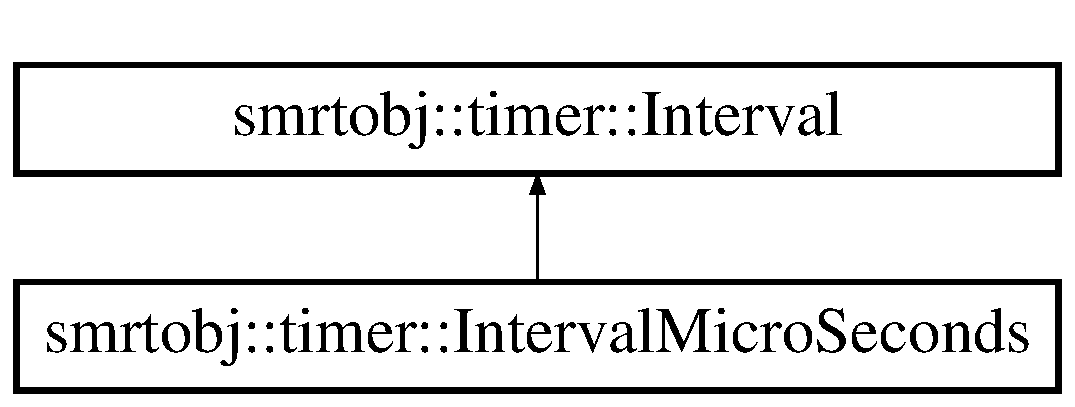
\includegraphics[height=2.000000cm]{classsmrtobj_1_1timer_1_1_interval_micro_seconds}
\end{center}
\end{figure}
\subsection*{Public Member Functions}
\begin{DoxyCompactItemize}
\item 
\hyperlink{classsmrtobj_1_1timer_1_1_interval_micro_seconds_a9dd6ff45eba9d3d2e972816086de056c}{Interval\+Micro\+Seconds} ()
\item 
\hyperlink{classsmrtobj_1_1timer_1_1_interval_micro_seconds_acb3760ee7ae1c2db2fd1a384aa444402}{Interval\+Micro\+Seconds} (unsigned long \hyperlink{classsmrtobj_1_1timer_1_1_interval_micro_seconds_afce0cbc55f0c884f0edb600ee3079ee9}{start})
\item 
\hyperlink{classsmrtobj_1_1timer_1_1_interval_micro_seconds_a1faf60520d61f2fb4ee551d79f9a52f4}{Interval\+Micro\+Seconds} (const \hyperlink{classsmrtobj_1_1timer_1_1_interval_micro_seconds}{Interval\+Micro\+Seconds} \&s)
\item 
virtual \hyperlink{classsmrtobj_1_1timer_1_1_interval_micro_seconds_a73131f274a84cf3fa7304c077dbc4314}{$\sim$\+Interval\+Micro\+Seconds} ()
\item 
void \hyperlink{classsmrtobj_1_1timer_1_1_interval_micro_seconds_a3e88ed37bc5cb4cbee0a745b040aaac5}{reset} (unsigned long \hyperlink{classsmrtobj_1_1timer_1_1_interval_micro_seconds_afce0cbc55f0c884f0edb600ee3079ee9}{start}=0)
\item 
virtual void \hyperlink{classsmrtobj_1_1timer_1_1_interval_micro_seconds_aa2679f2385f9e2182749ab696fa18ee6}{update} ()
\item 
unsigned long \hyperlink{classsmrtobj_1_1timer_1_1_interval_micro_seconds_afce0cbc55f0c884f0edb600ee3079ee9}{start} ()
\item 
virtual unsigned long \hyperlink{classsmrtobj_1_1timer_1_1_interval_micro_seconds_a583105ce23f3ffdefe31cbdccbb037c7}{time} ()
\item 
\hyperlink{classsmrtobj_1_1timer_1_1_interval_micro_seconds}{Interval\+Micro\+Seconds} \& \hyperlink{classsmrtobj_1_1timer_1_1_interval_micro_seconds_a4cd5de15337b6af42929f2c8c80d9b37}{operator=} (const \hyperlink{classsmrtobj_1_1timer_1_1_interval_micro_seconds}{Interval\+Micro\+Seconds} \&)
\end{DoxyCompactItemize}
\subsection*{Additional Inherited Members}


\subsection{Detailed Description}
The \hyperlink{classsmrtobj_1_1timer_1_1_interval_micro_seconds}{Interval\+Micro\+Seconds} class handles time intervals (in microseconds). This class inheritances from \hyperlink{classsmrtobj_1_1timer_1_1_interval_aaf7a279101cc8d105693107d9bdcb26a}{Interval} class. 

Definition at line 24 of file intervalmicroseconds.\+h.



\subsection{Constructor \& Destructor Documentation}
\hypertarget{classsmrtobj_1_1timer_1_1_interval_micro_seconds_a9dd6ff45eba9d3d2e972816086de056c}{}\index{smrtobj\+::timer\+::\+Interval\+Micro\+Seconds@{smrtobj\+::timer\+::\+Interval\+Micro\+Seconds}!Interval\+Micro\+Seconds@{Interval\+Micro\+Seconds}}
\index{Interval\+Micro\+Seconds@{Interval\+Micro\+Seconds}!smrtobj\+::timer\+::\+Interval\+Micro\+Seconds@{smrtobj\+::timer\+::\+Interval\+Micro\+Seconds}}
\subsubsection[{Interval\+Micro\+Seconds()}]{\setlength{\rightskip}{0pt plus 5cm}smrtobj\+::timer\+::\+Interval\+Micro\+Seconds\+::\+Interval\+Micro\+Seconds (
\begin{DoxyParamCaption}
{}
\end{DoxyParamCaption}
)}\label{classsmrtobj_1_1timer_1_1_interval_micro_seconds_a9dd6ff45eba9d3d2e972816086de056c}
Default Constructor 

Definition at line 18 of file intervalmicroseconds.\+cpp.

\hypertarget{classsmrtobj_1_1timer_1_1_interval_micro_seconds_acb3760ee7ae1c2db2fd1a384aa444402}{}\index{smrtobj\+::timer\+::\+Interval\+Micro\+Seconds@{smrtobj\+::timer\+::\+Interval\+Micro\+Seconds}!Interval\+Micro\+Seconds@{Interval\+Micro\+Seconds}}
\index{Interval\+Micro\+Seconds@{Interval\+Micro\+Seconds}!smrtobj\+::timer\+::\+Interval\+Micro\+Seconds@{smrtobj\+::timer\+::\+Interval\+Micro\+Seconds}}
\subsubsection[{Interval\+Micro\+Seconds(unsigned long start)}]{\setlength{\rightskip}{0pt plus 5cm}smrtobj\+::timer\+::\+Interval\+Micro\+Seconds\+::\+Interval\+Micro\+Seconds (
\begin{DoxyParamCaption}
\item[{unsigned long}]{start}
\end{DoxyParamCaption}
)}\label{classsmrtobj_1_1timer_1_1_interval_micro_seconds_acb3760ee7ae1c2db2fd1a384aa444402}
Constructor It sets the start time at a given value.


\begin{DoxyParams}[1]{Parameters}
\mbox{\tt in}  & {\em start} & start time \\
\hline
\end{DoxyParams}


Definition at line 23 of file intervalmicroseconds.\+cpp.

\hypertarget{classsmrtobj_1_1timer_1_1_interval_micro_seconds_a1faf60520d61f2fb4ee551d79f9a52f4}{}\index{smrtobj\+::timer\+::\+Interval\+Micro\+Seconds@{smrtobj\+::timer\+::\+Interval\+Micro\+Seconds}!Interval\+Micro\+Seconds@{Interval\+Micro\+Seconds}}
\index{Interval\+Micro\+Seconds@{Interval\+Micro\+Seconds}!smrtobj\+::timer\+::\+Interval\+Micro\+Seconds@{smrtobj\+::timer\+::\+Interval\+Micro\+Seconds}}
\subsubsection[{Interval\+Micro\+Seconds(const Interval\+Micro\+Seconds \&s)}]{\setlength{\rightskip}{0pt plus 5cm}smrtobj\+::timer\+::\+Interval\+Micro\+Seconds\+::\+Interval\+Micro\+Seconds (
\begin{DoxyParamCaption}
\item[{const {\bf Interval\+Micro\+Seconds} \&}]{s}
\end{DoxyParamCaption}
)}\label{classsmrtobj_1_1timer_1_1_interval_micro_seconds_a1faf60520d61f2fb4ee551d79f9a52f4}
Copy Constructor 

Definition at line 28 of file intervalmicroseconds.\+cpp.

\hypertarget{classsmrtobj_1_1timer_1_1_interval_micro_seconds_a73131f274a84cf3fa7304c077dbc4314}{}\index{smrtobj\+::timer\+::\+Interval\+Micro\+Seconds@{smrtobj\+::timer\+::\+Interval\+Micro\+Seconds}!````~Interval\+Micro\+Seconds@{$\sim$\+Interval\+Micro\+Seconds}}
\index{````~Interval\+Micro\+Seconds@{$\sim$\+Interval\+Micro\+Seconds}!smrtobj\+::timer\+::\+Interval\+Micro\+Seconds@{smrtobj\+::timer\+::\+Interval\+Micro\+Seconds}}
\subsubsection[{$\sim$\+Interval\+Micro\+Seconds()}]{\setlength{\rightskip}{0pt plus 5cm}smrtobj\+::timer\+::\+Interval\+Micro\+Seconds\+::$\sim$\+Interval\+Micro\+Seconds (
\begin{DoxyParamCaption}
{}
\end{DoxyParamCaption}
)\hspace{0.3cm}{\ttfamily [virtual]}}\label{classsmrtobj_1_1timer_1_1_interval_micro_seconds_a73131f274a84cf3fa7304c077dbc4314}
Destructor 

Definition at line 33 of file intervalmicroseconds.\+cpp.



\subsection{Member Function Documentation}
\hypertarget{classsmrtobj_1_1timer_1_1_interval_micro_seconds_a4cd5de15337b6af42929f2c8c80d9b37}{}\index{smrtobj\+::timer\+::\+Interval\+Micro\+Seconds@{smrtobj\+::timer\+::\+Interval\+Micro\+Seconds}!operator=@{operator=}}
\index{operator=@{operator=}!smrtobj\+::timer\+::\+Interval\+Micro\+Seconds@{smrtobj\+::timer\+::\+Interval\+Micro\+Seconds}}
\subsubsection[{operator=(const Interval\+Micro\+Seconds \&)}]{\setlength{\rightskip}{0pt plus 5cm}{\bf Interval\+Micro\+Seconds} \& smrtobj\+::timer\+::\+Interval\+Micro\+Seconds\+::operator= (
\begin{DoxyParamCaption}
\item[{const {\bf Interval\+Micro\+Seconds} \&}]{s}
\end{DoxyParamCaption}
)}\label{classsmrtobj_1_1timer_1_1_interval_micro_seconds_a4cd5de15337b6af42929f2c8c80d9b37}
Overload operator = 

Definition at line 37 of file intervalmicroseconds.\+cpp.

\hypertarget{classsmrtobj_1_1timer_1_1_interval_micro_seconds_a3e88ed37bc5cb4cbee0a745b040aaac5}{}\index{smrtobj\+::timer\+::\+Interval\+Micro\+Seconds@{smrtobj\+::timer\+::\+Interval\+Micro\+Seconds}!reset@{reset}}
\index{reset@{reset}!smrtobj\+::timer\+::\+Interval\+Micro\+Seconds@{smrtobj\+::timer\+::\+Interval\+Micro\+Seconds}}
\subsubsection[{reset(unsigned long start=0)}]{\setlength{\rightskip}{0pt plus 5cm}void smrtobj\+::timer\+::\+Interval\+Micro\+Seconds\+::reset (
\begin{DoxyParamCaption}
\item[{unsigned long}]{start = {\ttfamily 0}}
\end{DoxyParamCaption}
)}\label{classsmrtobj_1_1timer_1_1_interval_micro_seconds_a3e88ed37bc5cb4cbee0a745b040aaac5}
Resets the start time to now(). 

Definition at line 52 of file intervalmicroseconds.\+cpp.

\hypertarget{classsmrtobj_1_1timer_1_1_interval_micro_seconds_afce0cbc55f0c884f0edb600ee3079ee9}{}\index{smrtobj\+::timer\+::\+Interval\+Micro\+Seconds@{smrtobj\+::timer\+::\+Interval\+Micro\+Seconds}!start@{start}}
\index{start@{start}!smrtobj\+::timer\+::\+Interval\+Micro\+Seconds@{smrtobj\+::timer\+::\+Interval\+Micro\+Seconds}}
\subsubsection[{start()}]{\setlength{\rightskip}{0pt plus 5cm}unsigned long smrtobj\+::timer\+::\+Interval\+Micro\+Seconds\+::start (
\begin{DoxyParamCaption}
{}
\end{DoxyParamCaption}
)\hspace{0.3cm}{\ttfamily [inline]}}\label{classsmrtobj_1_1timer_1_1_interval_micro_seconds_afce0cbc55f0c884f0edb600ee3079ee9}
Returns the start time (in microseconds).

\begin{DoxyReturn}{Returns}
start time 
\end{DoxyReturn}


Definition at line 71 of file intervalmicroseconds.\+h.

\hypertarget{classsmrtobj_1_1timer_1_1_interval_micro_seconds_a583105ce23f3ffdefe31cbdccbb037c7}{}\index{smrtobj\+::timer\+::\+Interval\+Micro\+Seconds@{smrtobj\+::timer\+::\+Interval\+Micro\+Seconds}!time@{time}}
\index{time@{time}!smrtobj\+::timer\+::\+Interval\+Micro\+Seconds@{smrtobj\+::timer\+::\+Interval\+Micro\+Seconds}}
\subsubsection[{time()}]{\setlength{\rightskip}{0pt plus 5cm}unsigned long smrtobj\+::timer\+::\+Interval\+Micro\+Seconds\+::time (
\begin{DoxyParamCaption}
{}
\end{DoxyParamCaption}
)\hspace{0.3cm}{\ttfamily [virtual]}}\label{classsmrtobj_1_1timer_1_1_interval_micro_seconds_a583105ce23f3ffdefe31cbdccbb037c7}
Returns the time passed from the start time (in microseconds).

\begin{DoxyReturn}{Returns}
time passed 
\end{DoxyReturn}


Definition at line 46 of file intervalmicroseconds.\+cpp.

\hypertarget{classsmrtobj_1_1timer_1_1_interval_micro_seconds_aa2679f2385f9e2182749ab696fa18ee6}{}\index{smrtobj\+::timer\+::\+Interval\+Micro\+Seconds@{smrtobj\+::timer\+::\+Interval\+Micro\+Seconds}!update@{update}}
\index{update@{update}!smrtobj\+::timer\+::\+Interval\+Micro\+Seconds@{smrtobj\+::timer\+::\+Interval\+Micro\+Seconds}}
\subsubsection[{update()}]{\setlength{\rightskip}{0pt plus 5cm}virtual void smrtobj\+::timer\+::\+Interval\+Micro\+Seconds\+::update (
\begin{DoxyParamCaption}
{}
\end{DoxyParamCaption}
)\hspace{0.3cm}{\ttfamily [inline]}, {\ttfamily [virtual]}}\label{classsmrtobj_1_1timer_1_1_interval_micro_seconds_aa2679f2385f9e2182749ab696fa18ee6}
Updates the start time at current time. 

Definition at line 60 of file intervalmicroseconds.\+h.



The documentation for this class was generated from the following files\+:\begin{DoxyCompactItemize}
\item 
libraries/\+Smrt\+Obj\+Time/src/\hyperlink{intervalmicroseconds_8h}{intervalmicroseconds.\+h}\item 
libraries/\+Smrt\+Obj\+Time/src/intervalmicroseconds.\+cpp\end{DoxyCompactItemize}

\hypertarget{classsmrtobj_1_1timer_1_1_interval_seconds}{}\section{smrtobj\+:\+:timer\+:\+:Interval\+Seconds Class Reference}
\label{classsmrtobj_1_1timer_1_1_interval_seconds}\index{smrtobj\+::timer\+::\+Interval\+Seconds@{smrtobj\+::timer\+::\+Interval\+Seconds}}


{\ttfamily \#include $<$intervalseconds.\+h$>$}

Inheritance diagram for smrtobj\+:\+:timer\+:\+:Interval\+Seconds\+:\begin{figure}[H]
\begin{center}
\leavevmode
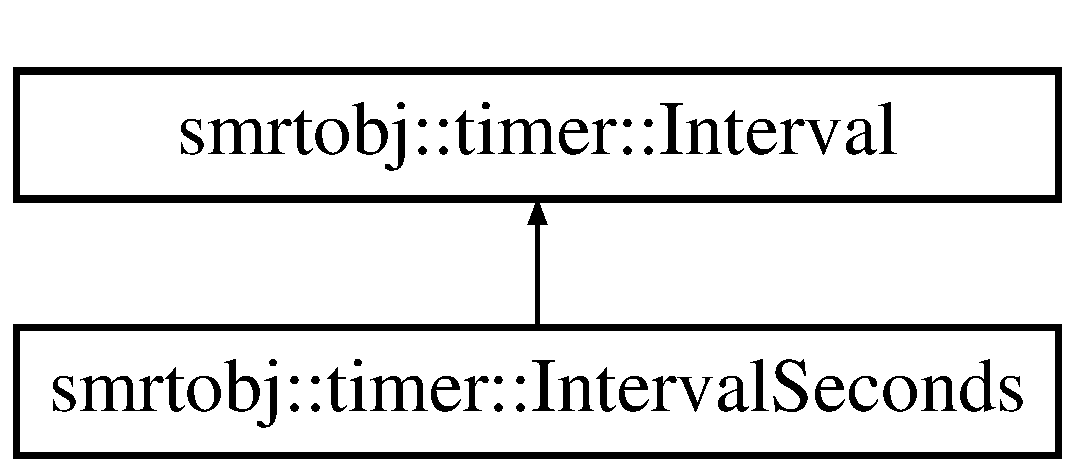
\includegraphics[height=2.000000cm]{classsmrtobj_1_1timer_1_1_interval_seconds}
\end{center}
\end{figure}
\subsection*{Public Types}
\begin{DoxyCompactItemize}
\item 
enum \hyperlink{classsmrtobj_1_1timer_1_1_interval_seconds_ab2187a2f2aab3fb8d6fcebba3680f764}{\+\_\+size} \{ \hyperlink{classsmrtobj_1_1timer_1_1_interval_seconds_ab2187a2f2aab3fb8d6fcebba3680f764af1f97577d8278e2e1b54551fafd67e0d}{S\+I\+Z\+E\+\_\+\+B\+U\+F\+F\+E\+R} = 20
 \}
\item 
enum \hyperlink{classsmrtobj_1_1timer_1_1_interval_seconds_a6ea1edd04e074d9fbaacee7ce297c7f8}{\+\_\+time\+\_\+format} \{ \hyperlink{classsmrtobj_1_1timer_1_1_interval_seconds_a6ea1edd04e074d9fbaacee7ce297c7f8a5e6def1fd27d935d55908db5ce04e808}{D\+E\+F\+A\+U\+L\+T\+\_\+\+T\+F} = 0, 
\hyperlink{classsmrtobj_1_1timer_1_1_interval_seconds_a6ea1edd04e074d9fbaacee7ce297c7f8a0993e789564a57e0bab49c5dad63be94}{E\+N} = 1, 
\hyperlink{classsmrtobj_1_1timer_1_1_interval_seconds_a6ea1edd04e074d9fbaacee7ce297c7f8a88d4402a7caafbd1e4383f0e40ec4b4b}{I\+O\+T} = 2
 \}
\end{DoxyCompactItemize}
\subsection*{Public Member Functions}
\begin{DoxyCompactItemize}
\item 
\hyperlink{classsmrtobj_1_1timer_1_1_interval_seconds_ac20f0f88661147329c47f397ca327900}{Interval\+Seconds} ()
\item 
\hyperlink{classsmrtobj_1_1timer_1_1_interval_seconds_ab6e29ed19bd3b68089c249fe16b62f42}{Interval\+Seconds} (unsigned long \hyperlink{classsmrtobj_1_1timer_1_1_interval_seconds_a1f8919a76123d44358ff32a1066c42b6}{start})
\item 
\hyperlink{classsmrtobj_1_1timer_1_1_interval_seconds_a3867300221f4967d7330c6ccced4813f}{Interval\+Seconds} (const \hyperlink{classsmrtobj_1_1timer_1_1_interval_seconds}{Interval\+Seconds} \&s)
\item 
virtual \hyperlink{classsmrtobj_1_1timer_1_1_interval_seconds_ac91271734ede29acfb795e4a0980f039}{$\sim$\+Interval\+Seconds} ()
\item 
void \hyperlink{classsmrtobj_1_1timer_1_1_interval_seconds_a0a2d997d360532f179a43c6d858afd37}{reset} (unsigned long \hyperlink{classsmrtobj_1_1timer_1_1_interval_seconds_a1f8919a76123d44358ff32a1066c42b6}{start})
\item 
virtual void \hyperlink{classsmrtobj_1_1timer_1_1_interval_seconds_a7253c7ab7b9e311dd13bbefbaa807c78}{update} ()
\item 
unsigned long \hyperlink{classsmrtobj_1_1timer_1_1_interval_seconds_a1f8919a76123d44358ff32a1066c42b6}{start} ()
\item 
virtual unsigned long \hyperlink{classsmrtobj_1_1timer_1_1_interval_seconds_a677364e751bbed28d85980f1270575a8}{time} ()
\item 
char $\ast$ \hyperlink{classsmrtobj_1_1timer_1_1_interval_seconds_ac4d08e03f84041a3132616b291c4c0ea}{get\+Time\+As\+String} (byte format=\hyperlink{classsmrtobj_1_1timer_1_1_interval_seconds_a6ea1edd04e074d9fbaacee7ce297c7f8a5e6def1fd27d935d55908db5ce04e808}{D\+E\+F\+A\+U\+L\+T\+\_\+\+T\+F})
\item 
\hyperlink{classsmrtobj_1_1timer_1_1_interval_seconds}{Interval\+Seconds} \& \hyperlink{classsmrtobj_1_1timer_1_1_interval_seconds_a2cc3e997f084e994bcf38494be513f02}{operator=} (const \hyperlink{classsmrtobj_1_1timer_1_1_interval_seconds}{Interval\+Seconds} \&)
\end{DoxyCompactItemize}
\subsection*{Additional Inherited Members}


\subsection{Detailed Description}
The \hyperlink{classsmrtobj_1_1timer_1_1_interval_seconds}{Interval\+Seconds} class handles time intervals (in seconds). This class inheritances from \hyperlink{classsmrtobj_1_1timer_1_1_interval_aaf7a279101cc8d105693107d9bdcb26a}{Interval} class. 

Definition at line 26 of file intervalseconds.\+h.



\subsection{Member Enumeration Documentation}
\hypertarget{classsmrtobj_1_1timer_1_1_interval_seconds_ab2187a2f2aab3fb8d6fcebba3680f764}{}\index{smrtobj\+::timer\+::\+Interval\+Seconds@{smrtobj\+::timer\+::\+Interval\+Seconds}!\+\_\+size@{\+\_\+size}}
\index{\+\_\+size@{\+\_\+size}!smrtobj\+::timer\+::\+Interval\+Seconds@{smrtobj\+::timer\+::\+Interval\+Seconds}}
\subsubsection[{\+\_\+size}]{\setlength{\rightskip}{0pt plus 5cm}enum {\bf smrtobj\+::timer\+::\+Interval\+Seconds\+::\+\_\+size}}\label{classsmrtobj_1_1timer_1_1_interval_seconds_ab2187a2f2aab3fb8d6fcebba3680f764}
Size of internal buffers \begin{Desc}
\item[Enumerator]\par
\begin{description}
\index{S\+I\+Z\+E\+\_\+\+B\+U\+F\+F\+E\+R@{S\+I\+Z\+E\+\_\+\+B\+U\+F\+F\+E\+R}!smrtobj\+::timer\+::\+Interval\+Seconds@{smrtobj\+::timer\+::\+Interval\+Seconds}}\index{smrtobj\+::timer\+::\+Interval\+Seconds@{smrtobj\+::timer\+::\+Interval\+Seconds}!S\+I\+Z\+E\+\_\+\+B\+U\+F\+F\+E\+R@{S\+I\+Z\+E\+\_\+\+B\+U\+F\+F\+E\+R}}\item[{\em 
\hypertarget{classsmrtobj_1_1timer_1_1_interval_seconds_ab2187a2f2aab3fb8d6fcebba3680f764af1f97577d8278e2e1b54551fafd67e0d}{}S\+I\+Z\+E\+\_\+\+B\+U\+F\+F\+E\+R\label{classsmrtobj_1_1timer_1_1_interval_seconds_ab2187a2f2aab3fb8d6fcebba3680f764af1f97577d8278e2e1b54551fafd67e0d}
}]Internal buffer size. \end{description}
\end{Desc}


Definition at line 34 of file intervalseconds.\+h.

\hypertarget{classsmrtobj_1_1timer_1_1_interval_seconds_a6ea1edd04e074d9fbaacee7ce297c7f8}{}\index{smrtobj\+::timer\+::\+Interval\+Seconds@{smrtobj\+::timer\+::\+Interval\+Seconds}!\+\_\+time\+\_\+format@{\+\_\+time\+\_\+format}}
\index{\+\_\+time\+\_\+format@{\+\_\+time\+\_\+format}!smrtobj\+::timer\+::\+Interval\+Seconds@{smrtobj\+::timer\+::\+Interval\+Seconds}}
\subsubsection[{\+\_\+time\+\_\+format}]{\setlength{\rightskip}{0pt plus 5cm}enum {\bf smrtobj\+::timer\+::\+Interval\+Seconds\+::\+\_\+time\+\_\+format}}\label{classsmrtobj_1_1timer_1_1_interval_seconds_a6ea1edd04e074d9fbaacee7ce297c7f8}
Time format \begin{Desc}
\item[Enumerator]\par
\begin{description}
\index{D\+E\+F\+A\+U\+L\+T\+\_\+\+T\+F@{D\+E\+F\+A\+U\+L\+T\+\_\+\+T\+F}!smrtobj\+::timer\+::\+Interval\+Seconds@{smrtobj\+::timer\+::\+Interval\+Seconds}}\index{smrtobj\+::timer\+::\+Interval\+Seconds@{smrtobj\+::timer\+::\+Interval\+Seconds}!D\+E\+F\+A\+U\+L\+T\+\_\+\+T\+F@{D\+E\+F\+A\+U\+L\+T\+\_\+\+T\+F}}\item[{\em 
\hypertarget{classsmrtobj_1_1timer_1_1_interval_seconds_a6ea1edd04e074d9fbaacee7ce297c7f8a5e6def1fd27d935d55908db5ce04e808}{}D\+E\+F\+A\+U\+L\+T\+\_\+\+T\+F\label{classsmrtobj_1_1timer_1_1_interval_seconds_a6ea1edd04e074d9fbaacee7ce297c7f8a5e6def1fd27d935d55908db5ce04e808}
}]Default format\+: D\+D/\+M\+M/\+Y\+Y\+Y\+Y hh\+:mm\+:ss. \index{E\+N@{E\+N}!smrtobj\+::timer\+::\+Interval\+Seconds@{smrtobj\+::timer\+::\+Interval\+Seconds}}\index{smrtobj\+::timer\+::\+Interval\+Seconds@{smrtobj\+::timer\+::\+Interval\+Seconds}!E\+N@{E\+N}}\item[{\em 
\hypertarget{classsmrtobj_1_1timer_1_1_interval_seconds_a6ea1edd04e074d9fbaacee7ce297c7f8a0993e789564a57e0bab49c5dad63be94}{}E\+N\label{classsmrtobj_1_1timer_1_1_interval_seconds_a6ea1edd04e074d9fbaacee7ce297c7f8a0993e789564a57e0bab49c5dad63be94}
}]English format\+: M\+M/\+D\+D/\+Y\+Y\+Y\+Y hh\+:mm\+:ss. \index{I\+O\+T@{I\+O\+T}!smrtobj\+::timer\+::\+Interval\+Seconds@{smrtobj\+::timer\+::\+Interval\+Seconds}}\index{smrtobj\+::timer\+::\+Interval\+Seconds@{smrtobj\+::timer\+::\+Interval\+Seconds}!I\+O\+T@{I\+O\+T}}\item[{\em 
\hypertarget{classsmrtobj_1_1timer_1_1_interval_seconds_a6ea1edd04e074d9fbaacee7ce297c7f8a88d4402a7caafbd1e4383f0e40ec4b4b}{}I\+O\+T\label{classsmrtobj_1_1timer_1_1_interval_seconds_a6ea1edd04e074d9fbaacee7ce297c7f8a88d4402a7caafbd1e4383f0e40ec4b4b}
}]Default format\+: M\+M/\+D\+D/\+Y\+Y\+Y\+Y hh\+:mm. \end{description}
\end{Desc}


Definition at line 45 of file intervalseconds.\+h.



\subsection{Constructor \& Destructor Documentation}
\hypertarget{classsmrtobj_1_1timer_1_1_interval_seconds_ac20f0f88661147329c47f397ca327900}{}\index{smrtobj\+::timer\+::\+Interval\+Seconds@{smrtobj\+::timer\+::\+Interval\+Seconds}!Interval\+Seconds@{Interval\+Seconds}}
\index{Interval\+Seconds@{Interval\+Seconds}!smrtobj\+::timer\+::\+Interval\+Seconds@{smrtobj\+::timer\+::\+Interval\+Seconds}}
\subsubsection[{Interval\+Seconds()}]{\setlength{\rightskip}{0pt plus 5cm}smrtobj\+::timer\+::\+Interval\+Seconds\+::\+Interval\+Seconds (
\begin{DoxyParamCaption}
{}
\end{DoxyParamCaption}
)}\label{classsmrtobj_1_1timer_1_1_interval_seconds_ac20f0f88661147329c47f397ca327900}
Default Constructor It sets all internal variables as the start time at current time as seconds from 1970. 

Definition at line 18 of file intervalseconds.\+cpp.

\hypertarget{classsmrtobj_1_1timer_1_1_interval_seconds_ab6e29ed19bd3b68089c249fe16b62f42}{}\index{smrtobj\+::timer\+::\+Interval\+Seconds@{smrtobj\+::timer\+::\+Interval\+Seconds}!Interval\+Seconds@{Interval\+Seconds}}
\index{Interval\+Seconds@{Interval\+Seconds}!smrtobj\+::timer\+::\+Interval\+Seconds@{smrtobj\+::timer\+::\+Interval\+Seconds}}
\subsubsection[{Interval\+Seconds(unsigned long start)}]{\setlength{\rightskip}{0pt plus 5cm}smrtobj\+::timer\+::\+Interval\+Seconds\+::\+Interval\+Seconds (
\begin{DoxyParamCaption}
\item[{unsigned long}]{start}
\end{DoxyParamCaption}
)}\label{classsmrtobj_1_1timer_1_1_interval_seconds_ab6e29ed19bd3b68089c249fe16b62f42}
Constructor It sets the start time at a given value.


\begin{DoxyParams}[1]{Parameters}
\mbox{\tt in}  & {\em start} & start time \\
\hline
\end{DoxyParams}


Definition at line 24 of file intervalseconds.\+cpp.

\hypertarget{classsmrtobj_1_1timer_1_1_interval_seconds_a3867300221f4967d7330c6ccced4813f}{}\index{smrtobj\+::timer\+::\+Interval\+Seconds@{smrtobj\+::timer\+::\+Interval\+Seconds}!Interval\+Seconds@{Interval\+Seconds}}
\index{Interval\+Seconds@{Interval\+Seconds}!smrtobj\+::timer\+::\+Interval\+Seconds@{smrtobj\+::timer\+::\+Interval\+Seconds}}
\subsubsection[{Interval\+Seconds(const Interval\+Seconds \&s)}]{\setlength{\rightskip}{0pt plus 5cm}smrtobj\+::timer\+::\+Interval\+Seconds\+::\+Interval\+Seconds (
\begin{DoxyParamCaption}
\item[{const {\bf Interval\+Seconds} \&}]{s}
\end{DoxyParamCaption}
)}\label{classsmrtobj_1_1timer_1_1_interval_seconds_a3867300221f4967d7330c6ccced4813f}
Copy Constructor 

Definition at line 30 of file intervalseconds.\+cpp.

\hypertarget{classsmrtobj_1_1timer_1_1_interval_seconds_ac91271734ede29acfb795e4a0980f039}{}\index{smrtobj\+::timer\+::\+Interval\+Seconds@{smrtobj\+::timer\+::\+Interval\+Seconds}!````~Interval\+Seconds@{$\sim$\+Interval\+Seconds}}
\index{````~Interval\+Seconds@{$\sim$\+Interval\+Seconds}!smrtobj\+::timer\+::\+Interval\+Seconds@{smrtobj\+::timer\+::\+Interval\+Seconds}}
\subsubsection[{$\sim$\+Interval\+Seconds()}]{\setlength{\rightskip}{0pt plus 5cm}smrtobj\+::timer\+::\+Interval\+Seconds\+::$\sim$\+Interval\+Seconds (
\begin{DoxyParamCaption}
{}
\end{DoxyParamCaption}
)\hspace{0.3cm}{\ttfamily [virtual]}}\label{classsmrtobj_1_1timer_1_1_interval_seconds_ac91271734ede29acfb795e4a0980f039}
Destructor 

Definition at line 36 of file intervalseconds.\+cpp.



\subsection{Member Function Documentation}
\hypertarget{classsmrtobj_1_1timer_1_1_interval_seconds_ac4d08e03f84041a3132616b291c4c0ea}{}\index{smrtobj\+::timer\+::\+Interval\+Seconds@{smrtobj\+::timer\+::\+Interval\+Seconds}!get\+Time\+As\+String@{get\+Time\+As\+String}}
\index{get\+Time\+As\+String@{get\+Time\+As\+String}!smrtobj\+::timer\+::\+Interval\+Seconds@{smrtobj\+::timer\+::\+Interval\+Seconds}}
\subsubsection[{get\+Time\+As\+String(byte format=\+D\+E\+F\+A\+U\+L\+T\+\_\+\+T\+F)}]{\setlength{\rightskip}{0pt plus 5cm}char $\ast$ smrtobj\+::timer\+::\+Interval\+Seconds\+::get\+Time\+As\+String (
\begin{DoxyParamCaption}
\item[{byte}]{format = {\ttfamily {\bf D\+E\+F\+A\+U\+L\+T\+\_\+\+T\+F}}}
\end{DoxyParamCaption}
)}\label{classsmrtobj_1_1timer_1_1_interval_seconds_ac4d08e03f84041a3132616b291c4c0ea}
Gets time in readable form as a string.


\begin{DoxyParams}[1]{Parameters}
\mbox{\tt in}  & {\em format} & format time accorting to \hyperlink{classsmrtobj_1_1timer_1_1_interval_seconds_a6ea1edd04e074d9fbaacee7ce297c7f8}{\+\_\+time\+\_\+format}\\
\hline
\end{DoxyParams}
\begin{DoxyReturn}{Returns}
time as a string 
\end{DoxyReturn}


Definition at line 65 of file intervalseconds.\+cpp.

\hypertarget{classsmrtobj_1_1timer_1_1_interval_seconds_a2cc3e997f084e994bcf38494be513f02}{}\index{smrtobj\+::timer\+::\+Interval\+Seconds@{smrtobj\+::timer\+::\+Interval\+Seconds}!operator=@{operator=}}
\index{operator=@{operator=}!smrtobj\+::timer\+::\+Interval\+Seconds@{smrtobj\+::timer\+::\+Interval\+Seconds}}
\subsubsection[{operator=(const Interval\+Seconds \&)}]{\setlength{\rightskip}{0pt plus 5cm}{\bf Interval\+Seconds} \& smrtobj\+::timer\+::\+Interval\+Seconds\+::operator= (
\begin{DoxyParamCaption}
\item[{const {\bf Interval\+Seconds} \&}]{s}
\end{DoxyParamCaption}
)}\label{classsmrtobj_1_1timer_1_1_interval_seconds_a2cc3e997f084e994bcf38494be513f02}
Overload operator = 

Definition at line 40 of file intervalseconds.\+cpp.

\hypertarget{classsmrtobj_1_1timer_1_1_interval_seconds_a0a2d997d360532f179a43c6d858afd37}{}\index{smrtobj\+::timer\+::\+Interval\+Seconds@{smrtobj\+::timer\+::\+Interval\+Seconds}!reset@{reset}}
\index{reset@{reset}!smrtobj\+::timer\+::\+Interval\+Seconds@{smrtobj\+::timer\+::\+Interval\+Seconds}}
\subsubsection[{reset(unsigned long start)}]{\setlength{\rightskip}{0pt plus 5cm}void smrtobj\+::timer\+::\+Interval\+Seconds\+::reset (
\begin{DoxyParamCaption}
\item[{unsigned long}]{start}
\end{DoxyParamCaption}
)}\label{classsmrtobj_1_1timer_1_1_interval_seconds_a0a2d997d360532f179a43c6d858afd37}
Resets the start time to now().


\begin{DoxyParams}[1]{Parameters}
\mbox{\tt in}  & {\em start} & start time \\
\hline
\end{DoxyParams}


Definition at line 53 of file intervalseconds.\+cpp.

\hypertarget{classsmrtobj_1_1timer_1_1_interval_seconds_a1f8919a76123d44358ff32a1066c42b6}{}\index{smrtobj\+::timer\+::\+Interval\+Seconds@{smrtobj\+::timer\+::\+Interval\+Seconds}!start@{start}}
\index{start@{start}!smrtobj\+::timer\+::\+Interval\+Seconds@{smrtobj\+::timer\+::\+Interval\+Seconds}}
\subsubsection[{start()}]{\setlength{\rightskip}{0pt plus 5cm}unsigned long smrtobj\+::timer\+::\+Interval\+Seconds\+::start (
\begin{DoxyParamCaption}
{}
\end{DoxyParamCaption}
)\hspace{0.3cm}{\ttfamily [inline]}}\label{classsmrtobj_1_1timer_1_1_interval_seconds_a1f8919a76123d44358ff32a1066c42b6}
Returns the start time (in seconds from 1970).

\begin{DoxyReturn}{Returns}
start time 
\end{DoxyReturn}


Definition at line 133 of file intervalseconds.\+h.

\hypertarget{classsmrtobj_1_1timer_1_1_interval_seconds_a677364e751bbed28d85980f1270575a8}{}\index{smrtobj\+::timer\+::\+Interval\+Seconds@{smrtobj\+::timer\+::\+Interval\+Seconds}!time@{time}}
\index{time@{time}!smrtobj\+::timer\+::\+Interval\+Seconds@{smrtobj\+::timer\+::\+Interval\+Seconds}}
\subsubsection[{time()}]{\setlength{\rightskip}{0pt plus 5cm}unsigned long smrtobj\+::timer\+::\+Interval\+Seconds\+::time (
\begin{DoxyParamCaption}
{}
\end{DoxyParamCaption}
)\hspace{0.3cm}{\ttfamily [virtual]}}\label{classsmrtobj_1_1timer_1_1_interval_seconds_a677364e751bbed28d85980f1270575a8}
Returns the time passed from the start time (in seconds).

\begin{DoxyReturn}{Returns}
time passed 
\end{DoxyReturn}


Definition at line 47 of file intervalseconds.\+cpp.

\hypertarget{classsmrtobj_1_1timer_1_1_interval_seconds_a7253c7ab7b9e311dd13bbefbaa807c78}{}\index{smrtobj\+::timer\+::\+Interval\+Seconds@{smrtobj\+::timer\+::\+Interval\+Seconds}!update@{update}}
\index{update@{update}!smrtobj\+::timer\+::\+Interval\+Seconds@{smrtobj\+::timer\+::\+Interval\+Seconds}}
\subsubsection[{update()}]{\setlength{\rightskip}{0pt plus 5cm}void smrtobj\+::timer\+::\+Interval\+Seconds\+::update (
\begin{DoxyParamCaption}
{}
\end{DoxyParamCaption}
)\hspace{0.3cm}{\ttfamily [inline]}, {\ttfamily [virtual]}}\label{classsmrtobj_1_1timer_1_1_interval_seconds_a7253c7ab7b9e311dd13bbefbaa807c78}
Updates the start time at current time. 

Definition at line 128 of file intervalseconds.\+h.



The documentation for this class was generated from the following files\+:\begin{DoxyCompactItemize}
\item 
libraries/\+Smrt\+Obj\+Time/src/intervalseconds.\+h\item 
libraries/\+Smrt\+Obj\+Time/src/intervalseconds.\+cpp\end{DoxyCompactItemize}

\hypertarget{classsmrtobj_1_1io_1_1_l_e_d_array}{}\section{smrtobj\+:\+:io\+:\+:L\+E\+D\+Array Class Reference}
\label{classsmrtobj_1_1io_1_1_l_e_d_array}\index{smrtobj\+::io\+::\+L\+E\+D\+Array@{smrtobj\+::io\+::\+L\+E\+D\+Array}}


{\ttfamily \#include $<$ledarray.\+h$>$}

\subsection*{Public Member Functions}
\begin{DoxyCompactItemize}
\item 
\hyperlink{classsmrtobj_1_1io_1_1_l_e_d_array_a456586cf665e9234fe5f9ba8a5e1afe7}{L\+E\+D\+Array} ()
\item 
\hyperlink{classsmrtobj_1_1io_1_1_l_e_d_array_a19b9dc0968a0df61ebff839855822c4a}{L\+E\+D\+Array} (const \hyperlink{classsmrtobj_1_1io_1_1_l_e_d_array}{L\+E\+D\+Array} \&l)
\item 
virtual \hyperlink{classsmrtobj_1_1io_1_1_l_e_d_array_aba3c59eefd537c438ab1684dfe09fca7}{$\sim$\+L\+E\+D\+Array} ()
\item 
byte \hyperlink{classsmrtobj_1_1io_1_1_l_e_d_array_acf2fc05accc35053a7d7987aeb9e4bed}{state} () const 
\item 
virtual bool \hyperlink{classsmrtobj_1_1io_1_1_l_e_d_array_a7fda2a4c901cf158beb7dc0e3c57cbe9}{check} ()=0
\item 
virtual bool \hyperlink{classsmrtobj_1_1io_1_1_l_e_d_array_a22376f08e9efc09bcb7a28fd797b8161}{attach} (\hyperlink{classsmrtobj_1_1io_1_1_digital_actuator}{Digital\+Actuator} \&led, byte pos)=0
\item 
virtual bool \hyperlink{classsmrtobj_1_1io_1_1_l_e_d_array_aaab58b896ed1ffafa272e7813d60d2bf}{change} (byte \hyperlink{classsmrtobj_1_1io_1_1_l_e_d_array_acf2fc05accc35053a7d7987aeb9e4bed}{state})=0
\end{DoxyCompactItemize}
\subsection*{Static Protected Member Functions}
\begin{DoxyCompactItemize}
\item 
static bool \hyperlink{classsmrtobj_1_1io_1_1_l_e_d_array_a162ff9d95114881a017bd7f11d3e1ac6}{check} (smrtobj\+::\+Digital\+Actuator $\ast$$\ast$leds\+Array, byte size)
\end{DoxyCompactItemize}
\subsection*{Protected Attributes}
\begin{DoxyCompactItemize}
\item 
\hypertarget{classsmrtobj_1_1io_1_1_l_e_d_array_aeb865e8cf9707498c97c57198da9c1a4}{}byte \hyperlink{classsmrtobj_1_1io_1_1_l_e_d_array_aeb865e8cf9707498c97c57198da9c1a4}{m\+\_\+state}\label{classsmrtobj_1_1io_1_1_l_e_d_array_aeb865e8cf9707498c97c57198da9c1a4}

\begin{DoxyCompactList}\small\item\em State of the L\+E\+D array. \end{DoxyCompactList}\end{DoxyCompactItemize}
\subsection*{Static Protected Attributes}
\begin{DoxyCompactItemize}
\item 
\hypertarget{classsmrtobj_1_1io_1_1_l_e_d_array_aec57c9c0fbdaa8250090f151e0f51d28}{}static const unsigned int \hyperlink{classsmrtobj_1_1io_1_1_l_e_d_array_aec57c9c0fbdaa8250090f151e0f51d28}{C\+H\+E\+C\+K\+\_\+\+T\+I\+M\+E} = 1000\label{classsmrtobj_1_1io_1_1_l_e_d_array_aec57c9c0fbdaa8250090f151e0f51d28}

\begin{DoxyCompactList}\small\item\em Time of blinking during the L\+E\+D array check. \end{DoxyCompactList}\end{DoxyCompactItemize}


\subsection{Detailed Description}
This class models an L\+E\+D array to give feedback about the state of the object. This is a abstract class.

To create an specific array of L\+E\+D, you have to create e new class, inheriting from \hyperlink{classsmrtobj_1_1io_1_1_l_e_d_array}{L\+E\+D\+Array} class and you have to redefine the functions\+:
\begin{DoxyItemize}
\item check;
\item attach;
\item change;
\end{DoxyItemize}

The new class have to define an array of pointer to \hyperlink{classsmrtobj_1_1io_1_1_digital_actuator}{Digital\+Actuator} object where each digital actuator is a L\+E\+D.~\newline
The function {\bfseries check} will call the static class function {\ttfamily check} using as arguments the array of \hyperlink{classsmrtobj_1_1io_1_1_digital_actuator}{Digital\+Actuator} pointer and the array size. The function \char`\"{}attach\char`\"{} will initialize the array at {\ttfamily pos} position, coping here the address of the \char`\"{}digital actuator\char`\"{} object. The function \char`\"{}chance\char`\"{} will change the state of L\+E\+D according to the state value. ~\newline
For example\+:


\begin{DoxyCode}
\textcolor{preprocessor}{#include <\hyperlink{smrtobjio_8h}{smrtobjio.h}>}

...

class MyLEDs: \textcolor{keyword}{public} smrtobj::LEDArray
\{
  \textcolor{keyword}{public}:
    \textcolor{keyword}{static} \textcolor{keyword}{const} byte N\_LEDS = 2;

    OutputLED();
    ~OutputLED();

    ...

    \textcolor{keyword}{virtual} \textcolor{keywordtype}{bool} \hyperlink{classsmrtobj_1_1io_1_1_l_e_d_array_a7fda2a4c901cf158beb7dc0e3c57cbe9}{check}();
    \textcolor{keyword}{virtual} \textcolor{keywordtype}{bool} \hyperlink{classsmrtobj_1_1io_1_1_l_e_d_array_a22376f08e9efc09bcb7a28fd797b8161}{attach}(smrtobj::DigitalActuator &led, byte pos);
    \textcolor{keyword}{virtual} \textcolor{keywordtype}{bool} \hyperlink{classsmrtobj_1_1io_1_1_l_e_d_array_aaab58b896ed1ffafa272e7813d60d2bf}{change}(byte state);

    \textcolor{keyword}{private}:
      smrtobj::DigitalActuator *m\_leds[N\_LEDS];
\}

\textcolor{keywordtype}{bool} MyLEDs::attach(smrtobj::DigitalActuator &led, byte pos)
\{
  m\_leds[pos] = &led;

  \textcolor{keywordflow}{return} \textcolor{keyword}{true};
\}

\textcolor{keywordtype}{bool} MyLEDs::check()
\{
  \textcolor{keywordflow}{return} StateLED::check(m\_leds, N\_LEDS);
\}

\textcolor{keywordtype}{bool} MyLEDs::change(byte state)
\{
  \textcolor{keywordflow}{switch} (state)
  \{
    \textcolor{keywordflow}{case} 0:
    \{
      \hyperlink{classsmrtobj_1_1io_1_1_l_e_d_array_aeb865e8cf9707498c97c57198da9c1a4}{m\_state} = \hyperlink{classsmrtobj_1_1io_1_1_l_e_d_array_acf2fc05accc35053a7d7987aeb9e4bed}{state};
      m\_leds[0]->off();
      m\_leds[1]->off();
    \}
    \textcolor{keywordflow}{break};
    \textcolor{keywordflow}{case} 1:
    \{
      \hyperlink{classsmrtobj_1_1io_1_1_l_e_d_array_aeb865e8cf9707498c97c57198da9c1a4}{m\_state} = \hyperlink{classsmrtobj_1_1io_1_1_l_e_d_array_acf2fc05accc35053a7d7987aeb9e4bed}{state};
      m\_leds[0]->off();
      m\_leds[1]->on();
    \}
    \textcolor{keywordflow}{break};
    \textcolor{keywordflow}{case} 2:
    \{
      \hyperlink{classsmrtobj_1_1io_1_1_l_e_d_array_aeb865e8cf9707498c97c57198da9c1a4}{m\_state} = \hyperlink{classsmrtobj_1_1io_1_1_l_e_d_array_acf2fc05accc35053a7d7987aeb9e4bed}{state};
      m\_leds[0]->on();
      m\_leds[1]->off();
    \}
    \textcolor{keywordflow}{break};
    \textcolor{keywordflow}{case} 3:
    \{
      \hyperlink{classsmrtobj_1_1io_1_1_l_e_d_array_aeb865e8cf9707498c97c57198da9c1a4}{m\_state} = \hyperlink{classsmrtobj_1_1io_1_1_l_e_d_array_acf2fc05accc35053a7d7987aeb9e4bed}{state};
      m\_leds[0]->on();
      m\_leds[1]->on();
    \}
    \textcolor{keywordflow}{break};
    \textcolor{keywordflow}{default}:
    \{
      \hyperlink{classsmrtobj_1_1io_1_1_l_e_d_array_aeb865e8cf9707498c97c57198da9c1a4}{m\_state} = \hyperlink{classsmrtobj_1_1io_1_1_l_e_d_array_acf2fc05accc35053a7d7987aeb9e4bed}{state};
      m\_leds[0]->off();
      m\_leds[1]->off();
    \}
  \}
  \textcolor{keywordflow}{return} \textcolor{keyword}{true};
\}
\end{DoxyCode}
 

Definition at line 123 of file ledarray.\+h.



\subsection{Constructor \& Destructor Documentation}
\hypertarget{classsmrtobj_1_1io_1_1_l_e_d_array_a456586cf665e9234fe5f9ba8a5e1afe7}{}\index{smrtobj\+::io\+::\+L\+E\+D\+Array@{smrtobj\+::io\+::\+L\+E\+D\+Array}!L\+E\+D\+Array@{L\+E\+D\+Array}}
\index{L\+E\+D\+Array@{L\+E\+D\+Array}!smrtobj\+::io\+::\+L\+E\+D\+Array@{smrtobj\+::io\+::\+L\+E\+D\+Array}}
\subsubsection[{L\+E\+D\+Array()}]{\setlength{\rightskip}{0pt plus 5cm}smrtobj\+::io\+::\+L\+E\+D\+Array\+::\+L\+E\+D\+Array (
\begin{DoxyParamCaption}
{}
\end{DoxyParamCaption}
)}\label{classsmrtobj_1_1io_1_1_l_e_d_array_a456586cf665e9234fe5f9ba8a5e1afe7}
Default Constructor. It initializes the state of the L\+E\+D array 

Definition at line 16 of file ledarray.\+cpp.

\hypertarget{classsmrtobj_1_1io_1_1_l_e_d_array_a19b9dc0968a0df61ebff839855822c4a}{}\index{smrtobj\+::io\+::\+L\+E\+D\+Array@{smrtobj\+::io\+::\+L\+E\+D\+Array}!L\+E\+D\+Array@{L\+E\+D\+Array}}
\index{L\+E\+D\+Array@{L\+E\+D\+Array}!smrtobj\+::io\+::\+L\+E\+D\+Array@{smrtobj\+::io\+::\+L\+E\+D\+Array}}
\subsubsection[{L\+E\+D\+Array(const L\+E\+D\+Array \&l)}]{\setlength{\rightskip}{0pt plus 5cm}smrtobj\+::io\+::\+L\+E\+D\+Array\+::\+L\+E\+D\+Array (
\begin{DoxyParamCaption}
\item[{const {\bf L\+E\+D\+Array} \&}]{l}
\end{DoxyParamCaption}
)}\label{classsmrtobj_1_1io_1_1_l_e_d_array_a19b9dc0968a0df61ebff839855822c4a}
Copy constructor. 

Definition at line 21 of file ledarray.\+cpp.

\hypertarget{classsmrtobj_1_1io_1_1_l_e_d_array_aba3c59eefd537c438ab1684dfe09fca7}{}\index{smrtobj\+::io\+::\+L\+E\+D\+Array@{smrtobj\+::io\+::\+L\+E\+D\+Array}!````~L\+E\+D\+Array@{$\sim$\+L\+E\+D\+Array}}
\index{````~L\+E\+D\+Array@{$\sim$\+L\+E\+D\+Array}!smrtobj\+::io\+::\+L\+E\+D\+Array@{smrtobj\+::io\+::\+L\+E\+D\+Array}}
\subsubsection[{$\sim$\+L\+E\+D\+Array()}]{\setlength{\rightskip}{0pt plus 5cm}smrtobj\+::io\+::\+L\+E\+D\+Array\+::$\sim$\+L\+E\+D\+Array (
\begin{DoxyParamCaption}
{}
\end{DoxyParamCaption}
)\hspace{0.3cm}{\ttfamily [virtual]}}\label{classsmrtobj_1_1io_1_1_l_e_d_array_aba3c59eefd537c438ab1684dfe09fca7}
Destructor. 

Definition at line 26 of file ledarray.\+cpp.



\subsection{Member Function Documentation}
\hypertarget{classsmrtobj_1_1io_1_1_l_e_d_array_a22376f08e9efc09bcb7a28fd797b8161}{}\index{smrtobj\+::io\+::\+L\+E\+D\+Array@{smrtobj\+::io\+::\+L\+E\+D\+Array}!attach@{attach}}
\index{attach@{attach}!smrtobj\+::io\+::\+L\+E\+D\+Array@{smrtobj\+::io\+::\+L\+E\+D\+Array}}
\subsubsection[{attach(\+Digital\+Actuator \&led, byte pos)=0}]{\setlength{\rightskip}{0pt plus 5cm}virtual bool smrtobj\+::io\+::\+L\+E\+D\+Array\+::attach (
\begin{DoxyParamCaption}
\item[{{\bf Digital\+Actuator} \&}]{led, }
\item[{byte}]{pos}
\end{DoxyParamCaption}
)\hspace{0.3cm}{\ttfamily [pure virtual]}}\label{classsmrtobj_1_1io_1_1_l_e_d_array_a22376f08e9efc09bcb7a28fd797b8161}
Attaches a new L\+E\+D (as a digital actuator) to the state L\+E\+D array.

\begin{DoxyReturn}{Returns}
true if no errors, false otherwise 
\end{DoxyReturn}
\hypertarget{classsmrtobj_1_1io_1_1_l_e_d_array_aaab58b896ed1ffafa272e7813d60d2bf}{}\index{smrtobj\+::io\+::\+L\+E\+D\+Array@{smrtobj\+::io\+::\+L\+E\+D\+Array}!change@{change}}
\index{change@{change}!smrtobj\+::io\+::\+L\+E\+D\+Array@{smrtobj\+::io\+::\+L\+E\+D\+Array}}
\subsubsection[{change(byte state)=0}]{\setlength{\rightskip}{0pt plus 5cm}virtual bool smrtobj\+::io\+::\+L\+E\+D\+Array\+::change (
\begin{DoxyParamCaption}
\item[{byte}]{state}
\end{DoxyParamCaption}
)\hspace{0.3cm}{\ttfamily [pure virtual]}}\label{classsmrtobj_1_1io_1_1_l_e_d_array_aaab58b896ed1ffafa272e7813d60d2bf}
Changes the L\+E\+Ds according the new state

\begin{DoxyReturn}{Returns}
true if no errors, false otherwise 
\end{DoxyReturn}
\hypertarget{classsmrtobj_1_1io_1_1_l_e_d_array_a162ff9d95114881a017bd7f11d3e1ac6}{}\index{smrtobj\+::io\+::\+L\+E\+D\+Array@{smrtobj\+::io\+::\+L\+E\+D\+Array}!check@{check}}
\index{check@{check}!smrtobj\+::io\+::\+L\+E\+D\+Array@{smrtobj\+::io\+::\+L\+E\+D\+Array}}
\subsubsection[{check(smrtobj\+::\+Digital\+Actuator $\ast$$\ast$leds\+Array, byte size)}]{\setlength{\rightskip}{0pt plus 5cm}bool smrtobj\+::io\+::\+L\+E\+D\+Array\+::check (
\begin{DoxyParamCaption}
\item[{smrtobj\+::\+Digital\+Actuator $\ast$$\ast$}]{leds\+Array, }
\item[{byte}]{size}
\end{DoxyParamCaption}
)\hspace{0.3cm}{\ttfamily [static]}, {\ttfamily [protected]}}\label{classsmrtobj_1_1io_1_1_l_e_d_array_a162ff9d95114881a017bd7f11d3e1ac6}
Its blinks a generic array of L\+E\+Ds. This operation can be used to check if all L\+E\+Ds are working correctly.


\begin{DoxyParams}[1]{Parameters}
\mbox{\tt in}  & {\em leds\+Array} & pointer to the L\+E\+D array \\
\hline
\mbox{\tt in}  & {\em size} & size of the L\+E\+D array \\
\hline
\end{DoxyParams}


Definition at line 30 of file ledarray.\+cpp.

\hypertarget{classsmrtobj_1_1io_1_1_l_e_d_array_a7fda2a4c901cf158beb7dc0e3c57cbe9}{}\index{smrtobj\+::io\+::\+L\+E\+D\+Array@{smrtobj\+::io\+::\+L\+E\+D\+Array}!check@{check}}
\index{check@{check}!smrtobj\+::io\+::\+L\+E\+D\+Array@{smrtobj\+::io\+::\+L\+E\+D\+Array}}
\subsubsection[{check()=0}]{\setlength{\rightskip}{0pt plus 5cm}virtual bool smrtobj\+::io\+::\+L\+E\+D\+Array\+::check (
\begin{DoxyParamCaption}
{}
\end{DoxyParamCaption}
)\hspace{0.3cm}{\ttfamily [pure virtual]}}\label{classsmrtobj_1_1io_1_1_l_e_d_array_a7fda2a4c901cf158beb7dc0e3c57cbe9}
Checks if all L\+E\+Ds works correctly, blinking them for \#smrtobj\+::\+L\+E\+D\+Array\+::\+C\+H\+E\+C\+K\+\_\+\+T\+I\+M\+E milliseconds

\begin{DoxyReturn}{Returns}
true if no errors, false otherwise 
\end{DoxyReturn}
\hypertarget{classsmrtobj_1_1io_1_1_l_e_d_array_acf2fc05accc35053a7d7987aeb9e4bed}{}\index{smrtobj\+::io\+::\+L\+E\+D\+Array@{smrtobj\+::io\+::\+L\+E\+D\+Array}!state@{state}}
\index{state@{state}!smrtobj\+::io\+::\+L\+E\+D\+Array@{smrtobj\+::io\+::\+L\+E\+D\+Array}}
\subsubsection[{state() const }]{\setlength{\rightskip}{0pt plus 5cm}byte smrtobj\+::io\+::\+L\+E\+D\+Array\+::state (
\begin{DoxyParamCaption}
{}
\end{DoxyParamCaption}
) const\hspace{0.3cm}{\ttfamily [inline]}}\label{classsmrtobj_1_1io_1_1_l_e_d_array_acf2fc05accc35053a7d7987aeb9e4bed}
Gets the current state of the L\+E\+D array

\begin{DoxyReturn}{Returns}
the current state of the L\+E\+D array 
\end{DoxyReturn}


Definition at line 165 of file ledarray.\+h.



The documentation for this class was generated from the following files\+:\begin{DoxyCompactItemize}
\item 
libraries/\+Smrt\+Obj\+I\+O/src/interfaces/\hyperlink{ledarray_8h}{ledarray.\+h}\item 
libraries/\+Smrt\+Obj\+I\+O/src/interfaces/\hyperlink{ledarray_8cpp}{ledarray.\+cpp}\end{DoxyCompactItemize}

\hypertarget{classsmrtobj_1_1io_1_1_m_c_p9700_a}{}\section{smrtobj\+:\+:io\+:\+:M\+C\+P9700\+A Class Reference}
\label{classsmrtobj_1_1io_1_1_m_c_p9700_a}\index{smrtobj\+::io\+::\+M\+C\+P9700\+A@{smrtobj\+::io\+::\+M\+C\+P9700\+A}}


{\ttfamily \#include $<$mcp9700a.\+h$>$}

Inheritance diagram for smrtobj\+:\+:io\+:\+:M\+C\+P9700\+A\+:\begin{figure}[H]
\begin{center}
\leavevmode
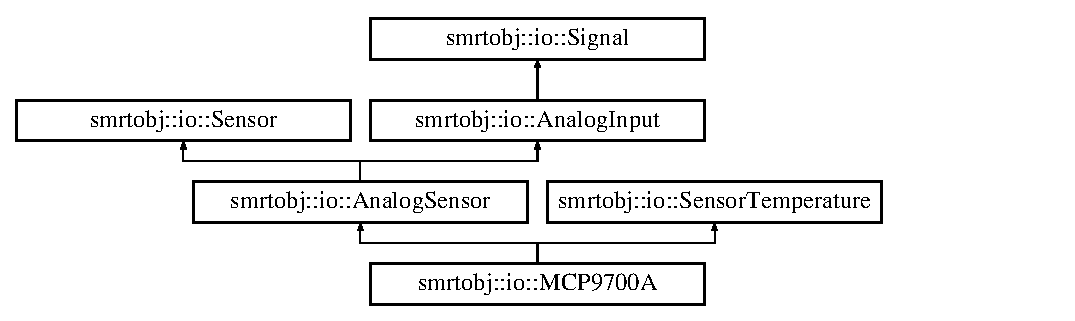
\includegraphics[height=3.868739cm]{classsmrtobj_1_1io_1_1_m_c_p9700_a}
\end{center}
\end{figure}
\subsection*{Public Member Functions}
\begin{DoxyCompactItemize}
\item 
\hyperlink{classsmrtobj_1_1io_1_1_m_c_p9700_a_a37975b91512826148e13fbc3301ba880}{M\+C\+P9700\+A} ()
\item 
\hyperlink{classsmrtobj_1_1io_1_1_m_c_p9700_a_a9ac9150fc7e74ae272984f254f34725e}{M\+C\+P9700\+A} (const \hyperlink{classsmrtobj_1_1io_1_1_m_c_p9700_a}{M\+C\+P9700\+A} \&s)
\item 
virtual \hyperlink{classsmrtobj_1_1io_1_1_m_c_p9700_a_a024fb11c7b84245d07b2f87ec1f35fa8}{$\sim$\+M\+C\+P9700\+A} ()
\item 
\hyperlink{classsmrtobj_1_1io_1_1_m_c_p9700_a}{M\+C\+P9700\+A} \& \hyperlink{classsmrtobj_1_1io_1_1_m_c_p9700_a_ad8bdad45ad4119634fad768ed0b0dd3c}{operator=} (const \hyperlink{classsmrtobj_1_1io_1_1_m_c_p9700_a}{M\+C\+P9700\+A} \&s)
\item 
virtual float \hyperlink{classsmrtobj_1_1io_1_1_m_c_p9700_a_ac80d2ee7705df843f6353f579be6f773}{celsius} ()
\item 
virtual float \hyperlink{classsmrtobj_1_1io_1_1_m_c_p9700_a_a5ed9f0c208b167fd8e4e1338062d8668}{kelvin} ()
\item 
virtual float \hyperlink{classsmrtobj_1_1io_1_1_m_c_p9700_a_a15dc548ff322a4e9f831273d96023038}{farenheit} ()
\item 
float \hyperlink{classsmrtobj_1_1io_1_1_m_c_p9700_a_ae50f36dae107dc570ad98646ba684a20}{read} ()
\end{DoxyCompactItemize}
\subsection*{Static Public Attributes}
\begin{DoxyCompactItemize}
\item 
\hypertarget{classsmrtobj_1_1io_1_1_m_c_p9700_a_a4c94b0a799b0ebe161faed70b6dcc9b7}{}static const float \hyperlink{classsmrtobj_1_1io_1_1_m_c_p9700_a_a4c94b0a799b0ebe161faed70b6dcc9b7}{Z\+E\+R\+O\+\_\+\+C\+\_\+\+V\+O\+L\+T\+S} = 0.\+50000\label{classsmrtobj_1_1io_1_1_m_c_p9700_a_a4c94b0a799b0ebe161faed70b6dcc9b7}

\begin{DoxyCompactList}\small\item\em Voltage at 0\+C (V\+D\+D = 5.\+0\+V) \end{DoxyCompactList}\item 
\hypertarget{classsmrtobj_1_1io_1_1_m_c_p9700_a_aaff6eec065bd28948e4eafc5792c51a3}{}static const float \hyperlink{classsmrtobj_1_1io_1_1_m_c_p9700_a_aaff6eec065bd28948e4eafc5792c51a3}{M\+V\+\_\+\+P\+E\+R\+\_\+\+D\+E\+G\+R\+E\+E\+\_\+\+C} = 0.\+01000\label{classsmrtobj_1_1io_1_1_m_c_p9700_a_aaff6eec065bd28948e4eafc5792c51a3}

\begin{DoxyCompactList}\small\item\em millivolts per degree Celsius (V\+D\+D = 5.\+0\+V) \end{DoxyCompactList}\end{DoxyCompactItemize}
\subsection*{Additional Inherited Members}


\subsection{Detailed Description}
Class \hyperlink{classsmrtobj_1_1io_1_1_m_c_p9700_a}{M\+C\+P9700\+A} models a temperature sensor (\hyperlink{classsmrtobj_1_1io_1_1_m_c_p9700_a}{M\+C\+P9700\+A}). Linear Active Thermistor™ I\+Cs are sensors whose output voltage is directly proportional to measured temperature. The \hyperlink{classsmrtobj_1_1io_1_1_m_c_p9700_a}{M\+C\+P9700\+A} can accurately measure temperature from -\/40\+C to +150\+C. The output of the \hyperlink{classsmrtobj_1_1io_1_1_m_c_p9700_a}{M\+C\+P9700\+A} is calibrated to a slope of 10m\+V/°\+C and has a D\+C offset of 500m\+V. The offset allows reading negative temperatures without the need for a negative supply. 

Definition at line 32 of file mcp9700a.\+h.



\subsection{Constructor \& Destructor Documentation}
\hypertarget{classsmrtobj_1_1io_1_1_m_c_p9700_a_a37975b91512826148e13fbc3301ba880}{}\index{smrtobj\+::io\+::\+M\+C\+P9700\+A@{smrtobj\+::io\+::\+M\+C\+P9700\+A}!M\+C\+P9700\+A@{M\+C\+P9700\+A}}
\index{M\+C\+P9700\+A@{M\+C\+P9700\+A}!smrtobj\+::io\+::\+M\+C\+P9700\+A@{smrtobj\+::io\+::\+M\+C\+P9700\+A}}
\subsubsection[{M\+C\+P9700\+A()}]{\setlength{\rightskip}{0pt plus 5cm}smrtobj\+::io\+::\+M\+C\+P9700\+A\+::\+M\+C\+P9700\+A (
\begin{DoxyParamCaption}
{}
\end{DoxyParamCaption}
)}\label{classsmrtobj_1_1io_1_1_m_c_p9700_a_a37975b91512826148e13fbc3301ba880}
Default Constructor. 

Definition at line 16 of file mcp9700a.\+cpp.

\hypertarget{classsmrtobj_1_1io_1_1_m_c_p9700_a_a9ac9150fc7e74ae272984f254f34725e}{}\index{smrtobj\+::io\+::\+M\+C\+P9700\+A@{smrtobj\+::io\+::\+M\+C\+P9700\+A}!M\+C\+P9700\+A@{M\+C\+P9700\+A}}
\index{M\+C\+P9700\+A@{M\+C\+P9700\+A}!smrtobj\+::io\+::\+M\+C\+P9700\+A@{smrtobj\+::io\+::\+M\+C\+P9700\+A}}
\subsubsection[{M\+C\+P9700\+A(const M\+C\+P9700\+A \&s)}]{\setlength{\rightskip}{0pt plus 5cm}smrtobj\+::io\+::\+M\+C\+P9700\+A\+::\+M\+C\+P9700\+A (
\begin{DoxyParamCaption}
\item[{const {\bf M\+C\+P9700\+A} \&}]{s}
\end{DoxyParamCaption}
)}\label{classsmrtobj_1_1io_1_1_m_c_p9700_a_a9ac9150fc7e74ae272984f254f34725e}
Copy Constructor.


\begin{DoxyParams}[1]{Parameters}
\mbox{\tt in}  & {\em s} & source sensor object \\
\hline
\end{DoxyParams}


Definition at line 23 of file mcp9700a.\+cpp.

\hypertarget{classsmrtobj_1_1io_1_1_m_c_p9700_a_a024fb11c7b84245d07b2f87ec1f35fa8}{}\index{smrtobj\+::io\+::\+M\+C\+P9700\+A@{smrtobj\+::io\+::\+M\+C\+P9700\+A}!````~M\+C\+P9700\+A@{$\sim$\+M\+C\+P9700\+A}}
\index{````~M\+C\+P9700\+A@{$\sim$\+M\+C\+P9700\+A}!smrtobj\+::io\+::\+M\+C\+P9700\+A@{smrtobj\+::io\+::\+M\+C\+P9700\+A}}
\subsubsection[{$\sim$\+M\+C\+P9700\+A()}]{\setlength{\rightskip}{0pt plus 5cm}smrtobj\+::io\+::\+M\+C\+P9700\+A\+::$\sim$\+M\+C\+P9700\+A (
\begin{DoxyParamCaption}
{}
\end{DoxyParamCaption}
)\hspace{0.3cm}{\ttfamily [virtual]}}\label{classsmrtobj_1_1io_1_1_m_c_p9700_a_a024fb11c7b84245d07b2f87ec1f35fa8}
Destructor. 

Definition at line 30 of file mcp9700a.\+cpp.



\subsection{Member Function Documentation}
\hypertarget{classsmrtobj_1_1io_1_1_m_c_p9700_a_ac80d2ee7705df843f6353f579be6f773}{}\index{smrtobj\+::io\+::\+M\+C\+P9700\+A@{smrtobj\+::io\+::\+M\+C\+P9700\+A}!celsius@{celsius}}
\index{celsius@{celsius}!smrtobj\+::io\+::\+M\+C\+P9700\+A@{smrtobj\+::io\+::\+M\+C\+P9700\+A}}
\subsubsection[{celsius()}]{\setlength{\rightskip}{0pt plus 5cm}float smrtobj\+::io\+::\+M\+C\+P9700\+A\+::celsius (
\begin{DoxyParamCaption}
{}
\end{DoxyParamCaption}
)\hspace{0.3cm}{\ttfamily [virtual]}}\label{classsmrtobj_1_1io_1_1_m_c_p9700_a_ac80d2ee7705df843f6353f579be6f773}
Gets temperature in celsius degrees

\begin{DoxyReturn}{Returns}
celsuius degrees 
\end{DoxyReturn}


Implements \hyperlink{classsmrtobj_1_1io_1_1_sensor_temperature_abea20003ad3b583d8f7b6021584afabe}{smrtobj\+::io\+::\+Sensor\+Temperature}.



Definition at line 43 of file mcp9700a.\+cpp.

\hypertarget{classsmrtobj_1_1io_1_1_m_c_p9700_a_a15dc548ff322a4e9f831273d96023038}{}\index{smrtobj\+::io\+::\+M\+C\+P9700\+A@{smrtobj\+::io\+::\+M\+C\+P9700\+A}!farenheit@{farenheit}}
\index{farenheit@{farenheit}!smrtobj\+::io\+::\+M\+C\+P9700\+A@{smrtobj\+::io\+::\+M\+C\+P9700\+A}}
\subsubsection[{farenheit()}]{\setlength{\rightskip}{0pt plus 5cm}float smrtobj\+::io\+::\+M\+C\+P9700\+A\+::farenheit (
\begin{DoxyParamCaption}
{}
\end{DoxyParamCaption}
)\hspace{0.3cm}{\ttfamily [virtual]}}\label{classsmrtobj_1_1io_1_1_m_c_p9700_a_a15dc548ff322a4e9f831273d96023038}
Gets temperature in farenheit degrees

\begin{DoxyReturn}{Returns}
farenheit degrees 
\end{DoxyReturn}


Implements \hyperlink{classsmrtobj_1_1io_1_1_sensor_temperature_a042ea89c32c26955d03186cc16e049b0}{smrtobj\+::io\+::\+Sensor\+Temperature}.



Definition at line 53 of file mcp9700a.\+cpp.

\hypertarget{classsmrtobj_1_1io_1_1_m_c_p9700_a_a5ed9f0c208b167fd8e4e1338062d8668}{}\index{smrtobj\+::io\+::\+M\+C\+P9700\+A@{smrtobj\+::io\+::\+M\+C\+P9700\+A}!kelvin@{kelvin}}
\index{kelvin@{kelvin}!smrtobj\+::io\+::\+M\+C\+P9700\+A@{smrtobj\+::io\+::\+M\+C\+P9700\+A}}
\subsubsection[{kelvin()}]{\setlength{\rightskip}{0pt plus 5cm}float smrtobj\+::io\+::\+M\+C\+P9700\+A\+::kelvin (
\begin{DoxyParamCaption}
{}
\end{DoxyParamCaption}
)\hspace{0.3cm}{\ttfamily [virtual]}}\label{classsmrtobj_1_1io_1_1_m_c_p9700_a_a5ed9f0c208b167fd8e4e1338062d8668}
Gets temperature in kelvin degrees

\begin{DoxyReturn}{Returns}
kelvin degrees 
\end{DoxyReturn}


Implements \hyperlink{classsmrtobj_1_1io_1_1_sensor_temperature_acd4a57d06be72757c3cdd5f1d14be117}{smrtobj\+::io\+::\+Sensor\+Temperature}.



Definition at line 48 of file mcp9700a.\+cpp.

\hypertarget{classsmrtobj_1_1io_1_1_m_c_p9700_a_ad8bdad45ad4119634fad768ed0b0dd3c}{}\index{smrtobj\+::io\+::\+M\+C\+P9700\+A@{smrtobj\+::io\+::\+M\+C\+P9700\+A}!operator=@{operator=}}
\index{operator=@{operator=}!smrtobj\+::io\+::\+M\+C\+P9700\+A@{smrtobj\+::io\+::\+M\+C\+P9700\+A}}
\subsubsection[{operator=(const M\+C\+P9700\+A \&s)}]{\setlength{\rightskip}{0pt plus 5cm}{\bf M\+C\+P9700\+A} \& smrtobj\+::io\+::\+M\+C\+P9700\+A\+::operator= (
\begin{DoxyParamCaption}
\item[{const {\bf M\+C\+P9700\+A} \&}]{s}
\end{DoxyParamCaption}
)}\label{classsmrtobj_1_1io_1_1_m_c_p9700_a_ad8bdad45ad4119634fad768ed0b0dd3c}
Override operator =


\begin{DoxyParams}[1]{Parameters}
\mbox{\tt in}  & {\em s} & source sensor object\\
\hline
\end{DoxyParams}
\begin{DoxyReturn}{Returns}
reference of the destination sensor 
\end{DoxyReturn}


Definition at line 34 of file mcp9700a.\+cpp.

\hypertarget{classsmrtobj_1_1io_1_1_m_c_p9700_a_ae50f36dae107dc570ad98646ba684a20}{}\index{smrtobj\+::io\+::\+M\+C\+P9700\+A@{smrtobj\+::io\+::\+M\+C\+P9700\+A}!read@{read}}
\index{read@{read}!smrtobj\+::io\+::\+M\+C\+P9700\+A@{smrtobj\+::io\+::\+M\+C\+P9700\+A}}
\subsubsection[{read()}]{\setlength{\rightskip}{0pt plus 5cm}float smrtobj\+::io\+::\+M\+C\+P9700\+A\+::read (
\begin{DoxyParamCaption}
{}
\end{DoxyParamCaption}
)\hspace{0.3cm}{\ttfamily [virtual]}}\label{classsmrtobj_1_1io_1_1_m_c_p9700_a_ae50f36dae107dc570ad98646ba684a20}
Reads value from the analog input

\begin{DoxyReturn}{Returns}
value as voltage 
\end{DoxyReturn}


Reimplemented from \hyperlink{classsmrtobj_1_1io_1_1_analog_sensor_a1084904f7f66c5f1e65b75ebdf3bf6b6}{smrtobj\+::io\+::\+Analog\+Sensor}.



Definition at line 58 of file mcp9700a.\+cpp.



The documentation for this class was generated from the following files\+:\begin{DoxyCompactItemize}
\item 
libraries/\+Smrt\+Obj\+I\+O/src/sensor/\hyperlink{mcp9700a_8h}{mcp9700a.\+h}\item 
libraries/\+Smrt\+Obj\+I\+O/src/sensor/\hyperlink{mcp9700a_8cpp}{mcp9700a.\+cpp}\end{DoxyCompactItemize}

\hypertarget{classsmrtobj_1_1io_1_1_output_device}{}\section{smrtobj\+:\+:io\+:\+:Output\+Device Class Reference}
\label{classsmrtobj_1_1io_1_1_output_device}\index{smrtobj\+::io\+::\+Output\+Device@{smrtobj\+::io\+::\+Output\+Device}}


{\ttfamily \#include $<$outputdevice.\+h$>$}

Inheritance diagram for smrtobj\+:\+:io\+:\+:Output\+Device\+:\begin{figure}[H]
\begin{center}
\leavevmode
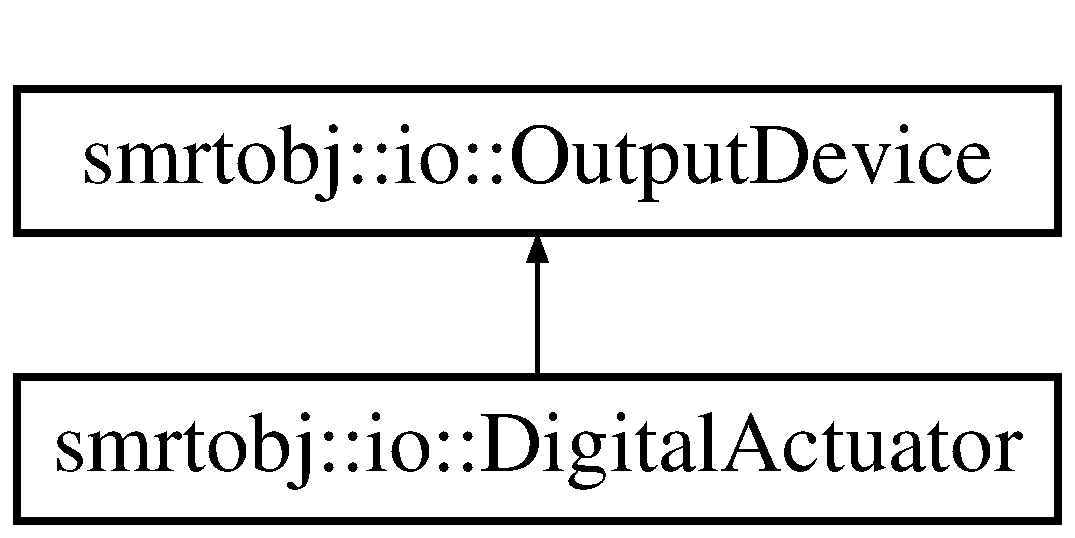
\includegraphics[height=2.000000cm]{classsmrtobj_1_1io_1_1_output_device}
\end{center}
\end{figure}
\subsection*{Public Types}
\begin{DoxyCompactItemize}
\item 
enum \hyperlink{classsmrtobj_1_1io_1_1_output_device_a0c8010d79d7229137e4669f855c3e18b}{\+\_\+state} \{ \hyperlink{classsmrtobj_1_1io_1_1_output_device_a0c8010d79d7229137e4669f855c3e18bac62cfce3ffab38b57bd81231f49ef59d}{O\+F\+F} = 0x00, 
\hyperlink{classsmrtobj_1_1io_1_1_output_device_a0c8010d79d7229137e4669f855c3e18ba28836c3fcc1c07cf6ee9a30a3ff53f94}{O\+N} = 0x01
 \}
\end{DoxyCompactItemize}
\subsection*{Public Member Functions}
\begin{DoxyCompactItemize}
\item 
\hyperlink{classsmrtobj_1_1io_1_1_output_device_a20a06b3b5cbaf8ff52118c2ef96c98ee}{Output\+Device} ()
\item 
virtual \hyperlink{classsmrtobj_1_1io_1_1_output_device_a184fef394e438e63b5b048cb302621c6}{$\sim$\+Output\+Device} ()
\item 
byte \hyperlink{classsmrtobj_1_1io_1_1_output_device_a4ad9f8f79001b7ad72be8faab9fe97a2}{state} ()
\item 
bool \hyperlink{classsmrtobj_1_1io_1_1_output_device_a0bf4746694296b538b22da4faa1ca4e3}{is\+On} ()
\item 
virtual bool \hyperlink{classsmrtobj_1_1io_1_1_output_device_a9154253249a8e95d69fa9d4ade592049}{on} ()=0
\item 
virtual bool \hyperlink{classsmrtobj_1_1io_1_1_output_device_a2700863f90da699cb82835ea6bb1f2f5}{off} ()=0
\end{DoxyCompactItemize}
\subsection*{Protected Attributes}
\begin{DoxyCompactItemize}
\item 
\hypertarget{classsmrtobj_1_1io_1_1_output_device_a269793861cb1a0fba566c70dfab3fafd}{}byte \hyperlink{classsmrtobj_1_1io_1_1_output_device_a269793861cb1a0fba566c70dfab3fafd}{m\+\_\+state}\label{classsmrtobj_1_1io_1_1_output_device_a269793861cb1a0fba566c70dfab3fafd}

\begin{DoxyCompactList}\small\item\em State of the actuator. It can be O\+N or O\+F\+F (\hyperlink{classsmrtobj_1_1io_1_1_output_device_a0c8010d79d7229137e4669f855c3e18b}{smrtobj\+::io\+::\+Output\+Device\+::\+\_\+state}) \end{DoxyCompactList}\end{DoxyCompactItemize}


\subsection{Detailed Description}
\hyperlink{classsmrtobj_1_1io_1_1_output_device}{Output\+Device} is an abstract class to model an interface for output signal connected to an actuator. 

Definition at line 22 of file outputdevice.\+h.



\subsection{Member Enumeration Documentation}
\hypertarget{classsmrtobj_1_1io_1_1_output_device_a0c8010d79d7229137e4669f855c3e18b}{}\index{smrtobj\+::io\+::\+Output\+Device@{smrtobj\+::io\+::\+Output\+Device}!\+\_\+state@{\+\_\+state}}
\index{\+\_\+state@{\+\_\+state}!smrtobj\+::io\+::\+Output\+Device@{smrtobj\+::io\+::\+Output\+Device}}
\subsubsection[{\+\_\+state}]{\setlength{\rightskip}{0pt plus 5cm}enum {\bf smrtobj\+::io\+::\+Output\+Device\+::\+\_\+state}}\label{classsmrtobj_1_1io_1_1_output_device_a0c8010d79d7229137e4669f855c3e18b}
State for an actuator \begin{Desc}
\item[Enumerator]\par
\begin{description}
\index{O\+F\+F@{O\+F\+F}!smrtobj\+::io\+::\+Output\+Device@{smrtobj\+::io\+::\+Output\+Device}}\index{smrtobj\+::io\+::\+Output\+Device@{smrtobj\+::io\+::\+Output\+Device}!O\+F\+F@{O\+F\+F}}\item[{\em 
\hypertarget{classsmrtobj_1_1io_1_1_output_device_a0c8010d79d7229137e4669f855c3e18bac62cfce3ffab38b57bd81231f49ef59d}{}O\+F\+F\label{classsmrtobj_1_1io_1_1_output_device_a0c8010d79d7229137e4669f855c3e18bac62cfce3ffab38b57bd81231f49ef59d}
}]Switched off. \index{O\+N@{O\+N}!smrtobj\+::io\+::\+Output\+Device@{smrtobj\+::io\+::\+Output\+Device}}\index{smrtobj\+::io\+::\+Output\+Device@{smrtobj\+::io\+::\+Output\+Device}!O\+N@{O\+N}}\item[{\em 
\hypertarget{classsmrtobj_1_1io_1_1_output_device_a0c8010d79d7229137e4669f855c3e18ba28836c3fcc1c07cf6ee9a30a3ff53f94}{}O\+N\label{classsmrtobj_1_1io_1_1_output_device_a0c8010d79d7229137e4669f855c3e18ba28836c3fcc1c07cf6ee9a30a3ff53f94}
}]Switched on. \end{description}
\end{Desc}


Definition at line 30 of file outputdevice.\+h.



\subsection{Constructor \& Destructor Documentation}
\hypertarget{classsmrtobj_1_1io_1_1_output_device_a20a06b3b5cbaf8ff52118c2ef96c98ee}{}\index{smrtobj\+::io\+::\+Output\+Device@{smrtobj\+::io\+::\+Output\+Device}!Output\+Device@{Output\+Device}}
\index{Output\+Device@{Output\+Device}!smrtobj\+::io\+::\+Output\+Device@{smrtobj\+::io\+::\+Output\+Device}}
\subsubsection[{Output\+Device()}]{\setlength{\rightskip}{0pt plus 5cm}smrtobj\+::\+Output\+Device\+::\+Output\+Device (
\begin{DoxyParamCaption}
{}
\end{DoxyParamCaption}
)}\label{classsmrtobj_1_1io_1_1_output_device_a20a06b3b5cbaf8ff52118c2ef96c98ee}
Default Constructor. It initializes the state of the actuator to switched off 

Definition at line 13 of file outputdevice.\+cpp.

\hypertarget{classsmrtobj_1_1io_1_1_output_device_a184fef394e438e63b5b048cb302621c6}{}\index{smrtobj\+::io\+::\+Output\+Device@{smrtobj\+::io\+::\+Output\+Device}!````~Output\+Device@{$\sim$\+Output\+Device}}
\index{````~Output\+Device@{$\sim$\+Output\+Device}!smrtobj\+::io\+::\+Output\+Device@{smrtobj\+::io\+::\+Output\+Device}}
\subsubsection[{$\sim$\+Output\+Device()}]{\setlength{\rightskip}{0pt plus 5cm}smrtobj\+::\+Output\+Device\+::$\sim$\+Output\+Device (
\begin{DoxyParamCaption}
{}
\end{DoxyParamCaption}
)\hspace{0.3cm}{\ttfamily [virtual]}}\label{classsmrtobj_1_1io_1_1_output_device_a184fef394e438e63b5b048cb302621c6}
Destructor. 

Definition at line 17 of file outputdevice.\+cpp.



\subsection{Member Function Documentation}
\hypertarget{classsmrtobj_1_1io_1_1_output_device_a0bf4746694296b538b22da4faa1ca4e3}{}\index{smrtobj\+::io\+::\+Output\+Device@{smrtobj\+::io\+::\+Output\+Device}!is\+On@{is\+On}}
\index{is\+On@{is\+On}!smrtobj\+::io\+::\+Output\+Device@{smrtobj\+::io\+::\+Output\+Device}}
\subsubsection[{is\+On()}]{\setlength{\rightskip}{0pt plus 5cm}bool smrtobj\+::io\+::\+Output\+Device\+::is\+On (
\begin{DoxyParamCaption}
{}
\end{DoxyParamCaption}
)\hspace{0.3cm}{\ttfamily [inline]}}\label{classsmrtobj_1_1io_1_1_output_device_a0bf4746694296b538b22da4faa1ca4e3}
Checks actuator state.

\begin{DoxyReturn}{Returns}
true if actuator is switched on, false otherwise 
\end{DoxyReturn}


Definition at line 63 of file outputdevice.\+h.

\hypertarget{classsmrtobj_1_1io_1_1_output_device_a2700863f90da699cb82835ea6bb1f2f5}{}\index{smrtobj\+::io\+::\+Output\+Device@{smrtobj\+::io\+::\+Output\+Device}!off@{off}}
\index{off@{off}!smrtobj\+::io\+::\+Output\+Device@{smrtobj\+::io\+::\+Output\+Device}}
\subsubsection[{off()=0}]{\setlength{\rightskip}{0pt plus 5cm}virtual bool smrtobj\+::io\+::\+Output\+Device\+::off (
\begin{DoxyParamCaption}
{}
\end{DoxyParamCaption}
)\hspace{0.3cm}{\ttfamily [pure virtual]}}\label{classsmrtobj_1_1io_1_1_output_device_a2700863f90da699cb82835ea6bb1f2f5}
Switches the actuator off

\begin{DoxyReturn}{Returns}
true if there are no errors, false otherwise 
\end{DoxyReturn}


Implemented in \hyperlink{classsmrtobj_1_1io_1_1_digital_actuator_aa5b6758d4bc05c9ae9ed666d62f65958}{smrtobj\+::io\+::\+Digital\+Actuator}.

\hypertarget{classsmrtobj_1_1io_1_1_output_device_a9154253249a8e95d69fa9d4ade592049}{}\index{smrtobj\+::io\+::\+Output\+Device@{smrtobj\+::io\+::\+Output\+Device}!on@{on}}
\index{on@{on}!smrtobj\+::io\+::\+Output\+Device@{smrtobj\+::io\+::\+Output\+Device}}
\subsubsection[{on()=0}]{\setlength{\rightskip}{0pt plus 5cm}virtual bool smrtobj\+::io\+::\+Output\+Device\+::on (
\begin{DoxyParamCaption}
{}
\end{DoxyParamCaption}
)\hspace{0.3cm}{\ttfamily [pure virtual]}}\label{classsmrtobj_1_1io_1_1_output_device_a9154253249a8e95d69fa9d4ade592049}
Switches the actuator on

\begin{DoxyReturn}{Returns}
true if there are no errors, false otherwise 
\end{DoxyReturn}


Implemented in \hyperlink{classsmrtobj_1_1io_1_1_digital_actuator_a2264475c4969b42e95118e73579d4d74}{smrtobj\+::io\+::\+Digital\+Actuator}.

\hypertarget{classsmrtobj_1_1io_1_1_output_device_a4ad9f8f79001b7ad72be8faab9fe97a2}{}\index{smrtobj\+::io\+::\+Output\+Device@{smrtobj\+::io\+::\+Output\+Device}!state@{state}}
\index{state@{state}!smrtobj\+::io\+::\+Output\+Device@{smrtobj\+::io\+::\+Output\+Device}}
\subsubsection[{state()}]{\setlength{\rightskip}{0pt plus 5cm}byte smrtobj\+::io\+::\+Output\+Device\+::state (
\begin{DoxyParamCaption}
{}
\end{DoxyParamCaption}
)\hspace{0.3cm}{\ttfamily [inline]}}\label{classsmrtobj_1_1io_1_1_output_device_a4ad9f8f79001b7ad72be8faab9fe97a2}
Gets the state of the actuator.

\begin{DoxyReturn}{Returns}
actuator state according to \hyperlink{classsmrtobj_1_1io_1_1_output_device_a0c8010d79d7229137e4669f855c3e18b}{\+\_\+state} enum 
\end{DoxyReturn}


Definition at line 56 of file outputdevice.\+h.



The documentation for this class was generated from the following files\+:\begin{DoxyCompactItemize}
\item 
libraries/\+Smrt\+Obj\+I\+O/src/interfaces/\hyperlink{outputdevice_8h}{outputdevice.\+h}\item 
libraries/\+Smrt\+Obj\+I\+O/src/interfaces/\hyperlink{outputdevice_8cpp}{outputdevice.\+cpp}\end{DoxyCompactItemize}

\hypertarget{classsmrtobj_1_1i2c_1_1_p_c_a9548_a}{}\section{smrtobj\+:\+:i2c\+:\+:P\+C\+A9548\+A Class Reference}
\label{classsmrtobj_1_1i2c_1_1_p_c_a9548_a}\index{smrtobj\+::i2c\+::\+P\+C\+A9548\+A@{smrtobj\+::i2c\+::\+P\+C\+A9548\+A}}


{\ttfamily \#include $<$P\+C\+A9548\+A.\+h$>$}

Inheritance diagram for smrtobj\+:\+:i2c\+:\+:P\+C\+A9548\+A\+:\begin{figure}[H]
\begin{center}
\leavevmode
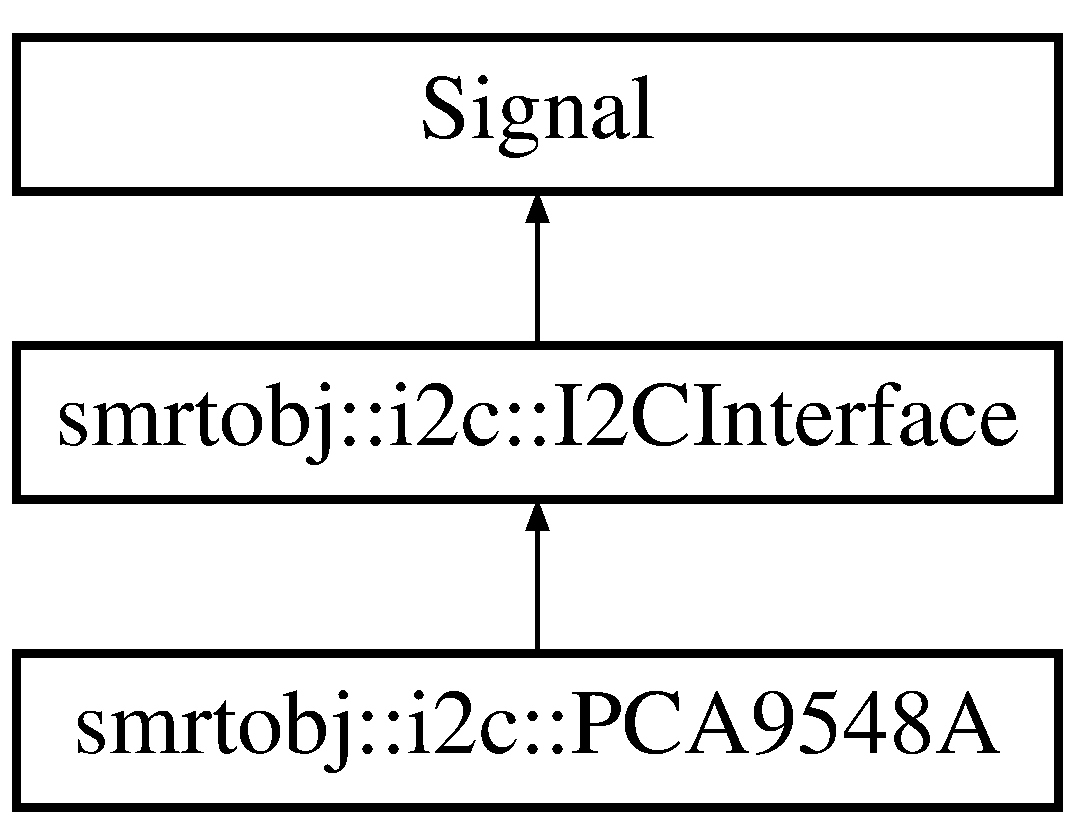
\includegraphics[height=3.000000cm]{classsmrtobj_1_1i2c_1_1_p_c_a9548_a}
\end{center}
\end{figure}
\subsection*{Public Types}
\begin{DoxyCompactItemize}
\item 
enum \hyperlink{classsmrtobj_1_1i2c_1_1_p_c_a9548_a_af9c75361cf8673778debf8a0822e1637}{\+\_\+device\+\_\+address} \{ {\bfseries D\+E\+V\+I\+C\+E\+\_\+\+A\+D\+D\+R\+E\+S\+S} = 0x70
 \}
\end{DoxyCompactItemize}
\subsection*{Public Member Functions}
\begin{DoxyCompactItemize}
\item 
\hyperlink{classsmrtobj_1_1i2c_1_1_p_c_a9548_a_a5da9ee25001c545a42d15f09ed540369}{P\+C\+A9548\+A} ()
\item 
\hyperlink{classsmrtobj_1_1i2c_1_1_p_c_a9548_a_af71a3d8fb553e56b261e9ae4f170c6cc}{P\+C\+A9548\+A} (uint8\+\_\+t addr)
\item 
\hyperlink{classsmrtobj_1_1i2c_1_1_p_c_a9548_a_a9cb4de3e7ce618a7a9eab948f964f65b}{P\+C\+A9548\+A} (const \hyperlink{classsmrtobj_1_1i2c_1_1_p_c_a9548_a}{P\+C\+A9548\+A} \&d)
\item 
virtual \hyperlink{classsmrtobj_1_1i2c_1_1_p_c_a9548_a_a1ca58fa8d04182e8a4331c2df22f8ff0}{$\sim$\+P\+C\+A9548\+A} ()
\item 
\hyperlink{classsmrtobj_1_1i2c_1_1_p_c_a9548_a}{P\+C\+A9548\+A} \& \hyperlink{classsmrtobj_1_1i2c_1_1_p_c_a9548_a_a3e4b0f941a2b34832a982c88c37daf98}{operator=} (const \hyperlink{classsmrtobj_1_1i2c_1_1_p_c_a9548_a}{P\+C\+A9548\+A} \&d)
\item 
virtual bool \hyperlink{classsmrtobj_1_1i2c_1_1_p_c_a9548_a_aad4b31d15abdf2514592b045530d82f3}{initialize} ()
\item 
virtual bool \hyperlink{classsmrtobj_1_1i2c_1_1_p_c_a9548_a_a2a697b995f40560498d2721a1e99e94a}{is\+Connected} ()
\item 
virtual bool \hyperlink{classsmrtobj_1_1i2c_1_1_p_c_a9548_a_af1dceb4c9b1cd4d4a1b15888ec793d38}{read} ()
\item 
uint8\+\_\+t \hyperlink{classsmrtobj_1_1i2c_1_1_p_c_a9548_a_a4f85bf0f2b6fd20f7c45a47daeabf337}{register\+Ctrl} ()
\item 
bool \hyperlink{classsmrtobj_1_1i2c_1_1_p_c_a9548_a_ac0f6f33e90b99a8cc83d1494ca0e69d9}{disable\+All} ()
\item 
bool \hyperlink{classsmrtobj_1_1i2c_1_1_p_c_a9548_a_af5f958d8cf301e98bf57eb6a6be4ee1a}{enable\+All} ()
\item 
bool \hyperlink{classsmrtobj_1_1i2c_1_1_p_c_a9548_a_a968beb6c12bfba1bbdb6b83ae69c11a0}{set\+Channel} (uint8\+\_\+t n, bool en)
\item 
bool \hyperlink{classsmrtobj_1_1i2c_1_1_p_c_a9548_a_ae500efb81c3a568d62b96777851f2b0e}{select} (uint8\+\_\+t n)
\end{DoxyCompactItemize}
\subsection*{Protected Member Functions}
\begin{DoxyCompactItemize}
\item 
bool \hyperlink{classsmrtobj_1_1i2c_1_1_p_c_a9548_a_ac2040afd2513758d699a9746bcbbccc1}{write} ()
\end{DoxyCompactItemize}
\subsection*{Additional Inherited Members}


\subsection{Detailed Description}
The \hyperlink{classsmrtobj_1_1i2c_1_1_p_c_a9548_a}{P\+C\+A9548\+A} has eight bidirectional translating switches that can be controlled via the I2\+C bus. The S\+C\+L/\+S\+D\+A upstream pair fans out to eight downstream pairs, or channels. Any individual S\+Cx/\+S\+Dx channel or combination of channels can be selected, determined by the contents of the programmable control register. The system master can reset the \hyperlink{classsmrtobj_1_1i2c_1_1_p_c_a9548_a}{P\+C\+A9548\+A} in the event of a timeout or other improper operation by asserting a low in the R\+E\+S\+E\+T input. Similarly, the power-\/on reset deselects all channels and initializes the I2\+C/\+S\+M\+Bus state machine. Asserting R\+E\+S\+E\+T causes the same reset/initialization to occur without powering down the part. 

Definition at line 26 of file P\+C\+A9548\+A.\+h.



\subsection{Member Enumeration Documentation}
\hypertarget{classsmrtobj_1_1i2c_1_1_p_c_a9548_a_af9c75361cf8673778debf8a0822e1637}{}\index{smrtobj\+::i2c\+::\+P\+C\+A9548\+A@{smrtobj\+::i2c\+::\+P\+C\+A9548\+A}!\+\_\+device\+\_\+address@{\+\_\+device\+\_\+address}}
\index{\+\_\+device\+\_\+address@{\+\_\+device\+\_\+address}!smrtobj\+::i2c\+::\+P\+C\+A9548\+A@{smrtobj\+::i2c\+::\+P\+C\+A9548\+A}}
\subsubsection[{\+\_\+device\+\_\+address}]{\setlength{\rightskip}{0pt plus 5cm}enum {\bf smrtobj\+::i2c\+::\+P\+C\+A9548\+A\+::\+\_\+device\+\_\+address}}\label{classsmrtobj_1_1i2c_1_1_p_c_a9548_a_af9c75361cf8673778debf8a0822e1637}
Device address used by default 

Definition at line 32 of file P\+C\+A9548\+A.\+h.



\subsection{Constructor \& Destructor Documentation}
\hypertarget{classsmrtobj_1_1i2c_1_1_p_c_a9548_a_a5da9ee25001c545a42d15f09ed540369}{}\index{smrtobj\+::i2c\+::\+P\+C\+A9548\+A@{smrtobj\+::i2c\+::\+P\+C\+A9548\+A}!P\+C\+A9548\+A@{P\+C\+A9548\+A}}
\index{P\+C\+A9548\+A@{P\+C\+A9548\+A}!smrtobj\+::i2c\+::\+P\+C\+A9548\+A@{smrtobj\+::i2c\+::\+P\+C\+A9548\+A}}
\subsubsection[{P\+C\+A9548\+A()}]{\setlength{\rightskip}{0pt plus 5cm}smrtobj\+::i2c\+::\+P\+C\+A9548\+A\+::\+P\+C\+A9548\+A (
\begin{DoxyParamCaption}
{}
\end{DoxyParamCaption}
)}\label{classsmrtobj_1_1i2c_1_1_p_c_a9548_a_a5da9ee25001c545a42d15f09ed540369}
Default Constructor. The {\itshape D\+E\+V\+I\+C\+E\+\_\+\+A\+D\+D\+R\+E\+S\+S} value of \hyperlink{classsmrtobj_1_1i2c_1_1_p_c_a9548_a_af9c75361cf8673778debf8a0822e1637}{smrtobj\+::i2c\+::\+P\+C\+A9548\+A\+::\+\_\+device\+\_\+address} is used as default address of the device. 

Definition at line 15 of file P\+C\+A9548\+A.\+cpp.

\hypertarget{classsmrtobj_1_1i2c_1_1_p_c_a9548_a_af71a3d8fb553e56b261e9ae4f170c6cc}{}\index{smrtobj\+::i2c\+::\+P\+C\+A9548\+A@{smrtobj\+::i2c\+::\+P\+C\+A9548\+A}!P\+C\+A9548\+A@{P\+C\+A9548\+A}}
\index{P\+C\+A9548\+A@{P\+C\+A9548\+A}!smrtobj\+::i2c\+::\+P\+C\+A9548\+A@{smrtobj\+::i2c\+::\+P\+C\+A9548\+A}}
\subsubsection[{P\+C\+A9548\+A(uint8\+\_\+t addr)}]{\setlength{\rightskip}{0pt plus 5cm}smrtobj\+::i2c\+::\+P\+C\+A9548\+A\+::\+P\+C\+A9548\+A (
\begin{DoxyParamCaption}
\item[{uint8\+\_\+t}]{addr}
\end{DoxyParamCaption}
)}\label{classsmrtobj_1_1i2c_1_1_p_c_a9548_a_af71a3d8fb553e56b261e9ae4f170c6cc}
Constructor. Sets the device address. It must be between 0x70 and 0x77. If value is not in this range, default value it is used ({\itshape D\+E\+V\+I\+C\+E\+\_\+\+A\+D\+D\+R\+E\+S\+S} value of \hyperlink{classsmrtobj_1_1i2c_1_1_p_c_a9548_a_af9c75361cf8673778debf8a0822e1637}{smrtobj\+::i2c\+::\+P\+C\+A9548\+A\+::\+\_\+device\+\_\+address}).


\begin{DoxyParams}[1]{Parameters}
\mbox{\tt in}  & {\em addr} & device address \\
\hline
\end{DoxyParams}


Definition at line 20 of file P\+C\+A9548\+A.\+cpp.

\hypertarget{classsmrtobj_1_1i2c_1_1_p_c_a9548_a_a9cb4de3e7ce618a7a9eab948f964f65b}{}\index{smrtobj\+::i2c\+::\+P\+C\+A9548\+A@{smrtobj\+::i2c\+::\+P\+C\+A9548\+A}!P\+C\+A9548\+A@{P\+C\+A9548\+A}}
\index{P\+C\+A9548\+A@{P\+C\+A9548\+A}!smrtobj\+::i2c\+::\+P\+C\+A9548\+A@{smrtobj\+::i2c\+::\+P\+C\+A9548\+A}}
\subsubsection[{P\+C\+A9548\+A(const P\+C\+A9548\+A \&d)}]{\setlength{\rightskip}{0pt plus 5cm}smrtobj\+::i2c\+::\+P\+C\+A9548\+A\+::\+P\+C\+A9548\+A (
\begin{DoxyParamCaption}
\item[{const {\bf P\+C\+A9548\+A} \&}]{d}
\end{DoxyParamCaption}
)}\label{classsmrtobj_1_1i2c_1_1_p_c_a9548_a_a9cb4de3e7ce618a7a9eab948f964f65b}
Copy Constructor.


\begin{DoxyParams}[1]{Parameters}
\mbox{\tt in}  & {\em d} & device object \\
\hline
\end{DoxyParams}


Definition at line 30 of file P\+C\+A9548\+A.\+cpp.

\hypertarget{classsmrtobj_1_1i2c_1_1_p_c_a9548_a_a1ca58fa8d04182e8a4331c2df22f8ff0}{}\index{smrtobj\+::i2c\+::\+P\+C\+A9548\+A@{smrtobj\+::i2c\+::\+P\+C\+A9548\+A}!````~P\+C\+A9548\+A@{$\sim$\+P\+C\+A9548\+A}}
\index{````~P\+C\+A9548\+A@{$\sim$\+P\+C\+A9548\+A}!smrtobj\+::i2c\+::\+P\+C\+A9548\+A@{smrtobj\+::i2c\+::\+P\+C\+A9548\+A}}
\subsubsection[{$\sim$\+P\+C\+A9548\+A()}]{\setlength{\rightskip}{0pt plus 5cm}smrtobj\+::i2c\+::\+P\+C\+A9548\+A\+::$\sim$\+P\+C\+A9548\+A (
\begin{DoxyParamCaption}
{}
\end{DoxyParamCaption}
)\hspace{0.3cm}{\ttfamily [virtual]}}\label{classsmrtobj_1_1i2c_1_1_p_c_a9548_a_a1ca58fa8d04182e8a4331c2df22f8ff0}
Destructor. 

Definition at line 35 of file P\+C\+A9548\+A.\+cpp.



\subsection{Member Function Documentation}
\hypertarget{classsmrtobj_1_1i2c_1_1_p_c_a9548_a_ac0f6f33e90b99a8cc83d1494ca0e69d9}{}\index{smrtobj\+::i2c\+::\+P\+C\+A9548\+A@{smrtobj\+::i2c\+::\+P\+C\+A9548\+A}!disable\+All@{disable\+All}}
\index{disable\+All@{disable\+All}!smrtobj\+::i2c\+::\+P\+C\+A9548\+A@{smrtobj\+::i2c\+::\+P\+C\+A9548\+A}}
\subsubsection[{disable\+All()}]{\setlength{\rightskip}{0pt plus 5cm}bool smrtobj\+::i2c\+::\+P\+C\+A9548\+A\+::disable\+All (
\begin{DoxyParamCaption}
{}
\end{DoxyParamCaption}
)\hspace{0.3cm}{\ttfamily [inline]}}\label{classsmrtobj_1_1i2c_1_1_p_c_a9548_a_ac0f6f33e90b99a8cc83d1494ca0e69d9}
Disables all channels. This function writes into control register value 0x00.

\begin{DoxyReturn}{Returns}
true for success, or false if any error occurs. 
\end{DoxyReturn}


Definition at line 119 of file P\+C\+A9548\+A.\+h.

\hypertarget{classsmrtobj_1_1i2c_1_1_p_c_a9548_a_af5f958d8cf301e98bf57eb6a6be4ee1a}{}\index{smrtobj\+::i2c\+::\+P\+C\+A9548\+A@{smrtobj\+::i2c\+::\+P\+C\+A9548\+A}!enable\+All@{enable\+All}}
\index{enable\+All@{enable\+All}!smrtobj\+::i2c\+::\+P\+C\+A9548\+A@{smrtobj\+::i2c\+::\+P\+C\+A9548\+A}}
\subsubsection[{enable\+All()}]{\setlength{\rightskip}{0pt plus 5cm}bool smrtobj\+::i2c\+::\+P\+C\+A9548\+A\+::enable\+All (
\begin{DoxyParamCaption}
{}
\end{DoxyParamCaption}
)\hspace{0.3cm}{\ttfamily [inline]}}\label{classsmrtobj_1_1i2c_1_1_p_c_a9548_a_af5f958d8cf301e98bf57eb6a6be4ee1a}
Enables all channels. This function writes into control register value 0x\+F\+F.

\begin{DoxyReturn}{Returns}
true for success, or false if any error occurs. 
\end{DoxyReturn}


Definition at line 126 of file P\+C\+A9548\+A.\+h.

\hypertarget{classsmrtobj_1_1i2c_1_1_p_c_a9548_a_aad4b31d15abdf2514592b045530d82f3}{}\index{smrtobj\+::i2c\+::\+P\+C\+A9548\+A@{smrtobj\+::i2c\+::\+P\+C\+A9548\+A}!initialize@{initialize}}
\index{initialize@{initialize}!smrtobj\+::i2c\+::\+P\+C\+A9548\+A@{smrtobj\+::i2c\+::\+P\+C\+A9548\+A}}
\subsubsection[{initialize()}]{\setlength{\rightskip}{0pt plus 5cm}bool smrtobj\+::i2c\+::\+P\+C\+A9548\+A\+::initialize (
\begin{DoxyParamCaption}
{}
\end{DoxyParamCaption}
)\hspace{0.3cm}{\ttfamily [virtual]}}\label{classsmrtobj_1_1i2c_1_1_p_c_a9548_a_aad4b31d15abdf2514592b045530d82f3}
Starts I2\+C communications. For this device, this function does nothing.

\begin{DoxyReturn}{Returns}
always true 
\end{DoxyReturn}


Implements \hyperlink{classsmrtobj_1_1i2c_1_1_i2_c_interface_a4ff1ff083d877c7c0816299b11965eb4}{smrtobj\+::i2c\+::\+I2\+C\+Interface}.



Definition at line 48 of file P\+C\+A9548\+A.\+cpp.

\hypertarget{classsmrtobj_1_1i2c_1_1_p_c_a9548_a_a2a697b995f40560498d2721a1e99e94a}{}\index{smrtobj\+::i2c\+::\+P\+C\+A9548\+A@{smrtobj\+::i2c\+::\+P\+C\+A9548\+A}!is\+Connected@{is\+Connected}}
\index{is\+Connected@{is\+Connected}!smrtobj\+::i2c\+::\+P\+C\+A9548\+A@{smrtobj\+::i2c\+::\+P\+C\+A9548\+A}}
\subsubsection[{is\+Connected()}]{\setlength{\rightskip}{0pt plus 5cm}bool smrtobj\+::i2c\+::\+P\+C\+A9548\+A\+::is\+Connected (
\begin{DoxyParamCaption}
{}
\end{DoxyParamCaption}
)\hspace{0.3cm}{\ttfamily [virtual]}}\label{classsmrtobj_1_1i2c_1_1_p_c_a9548_a_a2a697b995f40560498d2721a1e99e94a}
Tests if the device is connected. This function makes sure the device is connected and responds when you try to read a register.

\begin{DoxyReturn}{Returns}
true if connection is valid, false otherwise 
\end{DoxyReturn}


Implements \hyperlink{classsmrtobj_1_1i2c_1_1_i2_c_interface_a33fd37bafaf8c7e8184acb6470322bce}{smrtobj\+::i2c\+::\+I2\+C\+Interface}.



Definition at line 53 of file P\+C\+A9548\+A.\+cpp.

\hypertarget{classsmrtobj_1_1i2c_1_1_p_c_a9548_a_a3e4b0f941a2b34832a982c88c37daf98}{}\index{smrtobj\+::i2c\+::\+P\+C\+A9548\+A@{smrtobj\+::i2c\+::\+P\+C\+A9548\+A}!operator=@{operator=}}
\index{operator=@{operator=}!smrtobj\+::i2c\+::\+P\+C\+A9548\+A@{smrtobj\+::i2c\+::\+P\+C\+A9548\+A}}
\subsubsection[{operator=(const P\+C\+A9548\+A \&d)}]{\setlength{\rightskip}{0pt plus 5cm}{\bf P\+C\+A9548\+A} \& smrtobj\+::i2c\+::\+P\+C\+A9548\+A\+::operator= (
\begin{DoxyParamCaption}
\item[{const {\bf P\+C\+A9548\+A} \&}]{d}
\end{DoxyParamCaption}
)}\label{classsmrtobj_1_1i2c_1_1_p_c_a9548_a_a3e4b0f941a2b34832a982c88c37daf98}
Override operator =


\begin{DoxyParams}[1]{Parameters}
\mbox{\tt in}  & {\em d} & source device object\\
\hline
\end{DoxyParams}
\begin{DoxyReturn}{Returns}
destination obiect reference 
\end{DoxyReturn}


Definition at line 40 of file P\+C\+A9548\+A.\+cpp.

\hypertarget{classsmrtobj_1_1i2c_1_1_p_c_a9548_a_af1dceb4c9b1cd4d4a1b15888ec793d38}{}\index{smrtobj\+::i2c\+::\+P\+C\+A9548\+A@{smrtobj\+::i2c\+::\+P\+C\+A9548\+A}!read@{read}}
\index{read@{read}!smrtobj\+::i2c\+::\+P\+C\+A9548\+A@{smrtobj\+::i2c\+::\+P\+C\+A9548\+A}}
\subsubsection[{read()}]{\setlength{\rightskip}{0pt plus 5cm}bool smrtobj\+::i2c\+::\+P\+C\+A9548\+A\+::read (
\begin{DoxyParamCaption}
{}
\end{DoxyParamCaption}
)\hspace{0.3cm}{\ttfamily [virtual]}}\label{classsmrtobj_1_1i2c_1_1_p_c_a9548_a_af1dceb4c9b1cd4d4a1b15888ec793d38}
Reads the current value of the control register and saves it into internal buffer. To get the read time use function \hyperlink{classsmrtobj_1_1i2c_1_1_p_c_a9548_a_a4f85bf0f2b6fd20f7c45a47daeabf337}{smrtobj\+::i2c\+::\+P\+C\+A9548\+A\+::register\+Ctrl}.


\begin{DoxyCode}
\hyperlink{classsmrtobj_1_1i2c_1_1_p_c_a9548_a}{smrtobj::i2c::PCA9548A} i2c\_mux;

\textcolor{keywordflow}{if} ( i2c\_mux.\hyperlink{classsmrtobj_1_1i2c_1_1_p_c_a9548_a_af1dceb4c9b1cd4d4a1b15888ec793d38}{read}() )
\{
  uint8\_t reg = i2c\_mux.time();
  ...
\} 
\end{DoxyCode}


\begin{DoxyReturn}{Returns}
true for success, or false if any error occurs. 
\end{DoxyReturn}


Implements \hyperlink{classsmrtobj_1_1i2c_1_1_i2_c_interface_a58bc734662a60de6a7cb7976c2179753}{smrtobj\+::i2c\+::\+I2\+C\+Interface}.



Definition at line 58 of file P\+C\+A9548\+A.\+cpp.

\hypertarget{classsmrtobj_1_1i2c_1_1_p_c_a9548_a_a4f85bf0f2b6fd20f7c45a47daeabf337}{}\index{smrtobj\+::i2c\+::\+P\+C\+A9548\+A@{smrtobj\+::i2c\+::\+P\+C\+A9548\+A}!register\+Ctrl@{register\+Ctrl}}
\index{register\+Ctrl@{register\+Ctrl}!smrtobj\+::i2c\+::\+P\+C\+A9548\+A@{smrtobj\+::i2c\+::\+P\+C\+A9548\+A}}
\subsubsection[{register\+Ctrl()}]{\setlength{\rightskip}{0pt plus 5cm}uint8\+\_\+t smrtobj\+::i2c\+::\+P\+C\+A9548\+A\+::register\+Ctrl (
\begin{DoxyParamCaption}
{}
\end{DoxyParamCaption}
)\hspace{0.3cm}{\ttfamily [inline]}}\label{classsmrtobj_1_1i2c_1_1_p_c_a9548_a_a4f85bf0f2b6fd20f7c45a47daeabf337}
Gets the last value read of the control register.

\begin{DoxyReturn}{Returns}
last value read. 
\end{DoxyReturn}


Definition at line 112 of file P\+C\+A9548\+A.\+h.

\hypertarget{classsmrtobj_1_1i2c_1_1_p_c_a9548_a_ae500efb81c3a568d62b96777851f2b0e}{}\index{smrtobj\+::i2c\+::\+P\+C\+A9548\+A@{smrtobj\+::i2c\+::\+P\+C\+A9548\+A}!select@{select}}
\index{select@{select}!smrtobj\+::i2c\+::\+P\+C\+A9548\+A@{smrtobj\+::i2c\+::\+P\+C\+A9548\+A}}
\subsubsection[{select(uint8\+\_\+t n)}]{\setlength{\rightskip}{0pt plus 5cm}bool smrtobj\+::i2c\+::\+P\+C\+A9548\+A\+::select (
\begin{DoxyParamCaption}
\item[{uint8\+\_\+t}]{n}
\end{DoxyParamCaption}
)}\label{classsmrtobj_1_1i2c_1_1_p_c_a9548_a_ae500efb81c3a568d62b96777851f2b0e}
Selects only a specific channel.


\begin{DoxyParams}[1]{Parameters}
\mbox{\tt in}  & {\em n} & channel number\\
\hline
\end{DoxyParams}
\begin{DoxyReturn}{Returns}
true for success, or false if any error occurs. 
\end{DoxyReturn}


Definition at line 86 of file P\+C\+A9548\+A.\+cpp.

\hypertarget{classsmrtobj_1_1i2c_1_1_p_c_a9548_a_a968beb6c12bfba1bbdb6b83ae69c11a0}{}\index{smrtobj\+::i2c\+::\+P\+C\+A9548\+A@{smrtobj\+::i2c\+::\+P\+C\+A9548\+A}!set\+Channel@{set\+Channel}}
\index{set\+Channel@{set\+Channel}!smrtobj\+::i2c\+::\+P\+C\+A9548\+A@{smrtobj\+::i2c\+::\+P\+C\+A9548\+A}}
\subsubsection[{set\+Channel(uint8\+\_\+t n, bool en)}]{\setlength{\rightskip}{0pt plus 5cm}bool smrtobj\+::i2c\+::\+P\+C\+A9548\+A\+::set\+Channel (
\begin{DoxyParamCaption}
\item[{uint8\+\_\+t}]{n, }
\item[{bool}]{en}
\end{DoxyParamCaption}
)}\label{classsmrtobj_1_1i2c_1_1_p_c_a9548_a_a968beb6c12bfba1bbdb6b83ae69c11a0}
Sets the state (enable/disable) of a channel.


\begin{DoxyParams}[1]{Parameters}
\mbox{\tt in}  & {\em n} & channel number \\
\hline
\mbox{\tt in}  & {\em en} & 0 to disable, 1 to enable\\
\hline
\end{DoxyParams}
\begin{DoxyReturn}{Returns}
true for success, or false if any error occurs. 
\end{DoxyReturn}


Definition at line 68 of file P\+C\+A9548\+A.\+cpp.

\hypertarget{classsmrtobj_1_1i2c_1_1_p_c_a9548_a_ac2040afd2513758d699a9746bcbbccc1}{}\index{smrtobj\+::i2c\+::\+P\+C\+A9548\+A@{smrtobj\+::i2c\+::\+P\+C\+A9548\+A}!write@{write}}
\index{write@{write}!smrtobj\+::i2c\+::\+P\+C\+A9548\+A@{smrtobj\+::i2c\+::\+P\+C\+A9548\+A}}
\subsubsection[{write()}]{\setlength{\rightskip}{0pt plus 5cm}bool smrtobj\+::i2c\+::\+P\+C\+A9548\+A\+::write (
\begin{DoxyParamCaption}
{}
\end{DoxyParamCaption}
)\hspace{0.3cm}{\ttfamily [protected]}}\label{classsmrtobj_1_1i2c_1_1_p_c_a9548_a_ac2040afd2513758d699a9746bcbbccc1}
Writes the control register, using value saved into a internal buffer.

\begin{DoxyReturn}{Returns}
true for success, or false if any error occurs. 
\end{DoxyReturn}


Definition at line 63 of file P\+C\+A9548\+A.\+cpp.



The documentation for this class was generated from the following files\+:\begin{DoxyCompactItemize}
\item 
libraries/\+Smrt\+Obj\+I2\+C/src/devices/\hyperlink{_p_c_a9548_a_8h}{P\+C\+A9548\+A.\+h}\item 
libraries/\+Smrt\+Obj\+I2\+C/src/devices/P\+C\+A9548\+A.\+cpp\end{DoxyCompactItemize}

\hypertarget{classsmrtobj_1_1io_1_1_p_w_m_output}{}\section{smrtobj\+:\+:io\+:\+:P\+W\+M\+Output Class Reference}
\label{classsmrtobj_1_1io_1_1_p_w_m_output}\index{smrtobj\+::io\+::\+P\+W\+M\+Output@{smrtobj\+::io\+::\+P\+W\+M\+Output}}


{\ttfamily \#include $<$iosignal.\+h$>$}

Inheritance diagram for smrtobj\+:\+:io\+:\+:P\+W\+M\+Output\+:\begin{figure}[H]
\begin{center}
\leavevmode
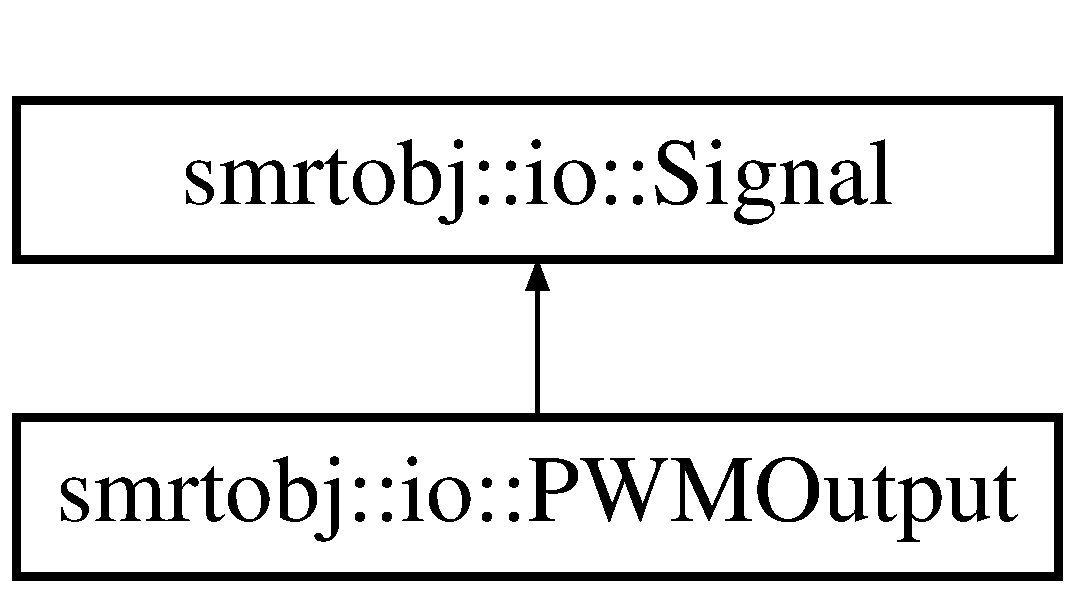
\includegraphics[height=2.000000cm]{classsmrtobj_1_1io_1_1_p_w_m_output}
\end{center}
\end{figure}
\subsection*{Public Member Functions}
\begin{DoxyCompactItemize}
\item 
\hyperlink{classsmrtobj_1_1io_1_1_p_w_m_output_adea97b12a8895b84b9cc0a056520770c}{P\+W\+M\+Output} ()
\item 
\hyperlink{classsmrtobj_1_1io_1_1_p_w_m_output_a848a4fc96ebdbb579d34b63fb152dfdd}{P\+W\+M\+Output} (const \hyperlink{classsmrtobj_1_1io_1_1_p_w_m_output}{P\+W\+M\+Output} \&o)
\item 
virtual \hyperlink{classsmrtobj_1_1io_1_1_p_w_m_output_aaf792a72ce1d9de754fce790f852b5c3}{$\sim$\+P\+W\+M\+Output} ()
\item 
\hyperlink{classsmrtobj_1_1io_1_1_p_w_m_output}{P\+W\+M\+Output} \& \hyperlink{classsmrtobj_1_1io_1_1_p_w_m_output_ad204d0cf31273a0160914de56a1c3b0c}{operator=} (const \hyperlink{classsmrtobj_1_1io_1_1_p_w_m_output}{P\+W\+M\+Output} \&o)
\item 
byte \hyperlink{classsmrtobj_1_1io_1_1_p_w_m_output_ac5908c2317a1e2e7a293f8ee04d42a77}{type} ()
\item 
void \hyperlink{classsmrtobj_1_1io_1_1_p_w_m_output_a10f8b63f2769f41df9abde0872ef209f}{init} (byte \hyperlink{classsmrtobj_1_1io_1_1_p_w_m_output_a310d81c32649b121c6a2b02173986e96}{pin})
\item 
byte \hyperlink{classsmrtobj_1_1io_1_1_p_w_m_output_a19bc1ccc705b00198425c587e433b2d9}{value} ()
\item 
byte \hyperlink{classsmrtobj_1_1io_1_1_p_w_m_output_a310d81c32649b121c6a2b02173986e96}{pin} ()
\item 
bool \hyperlink{classsmrtobj_1_1io_1_1_p_w_m_output_ac49273d0fbe3419c064509a068e6e667}{write} (byte \hyperlink{classsmrtobj_1_1io_1_1_p_w_m_output_a19bc1ccc705b00198425c587e433b2d9}{value})
\end{DoxyCompactItemize}
\subsection*{Additional Inherited Members}


\subsection{Detailed Description}
The \hyperlink{classsmrtobj_1_1io_1_1_p_w_m_output}{P\+W\+M\+Output} class models a P\+W\+M (Pulse Width Modulation) output. It can be used to light a L\+E\+D at varying brightnesses or drive a motor at various speeds. Writing a value, the pin will generate a steady square wave of the specified duty cycle. This is achieved by {\bfseries analog\+Write} function. P\+W\+M duty-\/cycle is between 0 (always off) and 255 (always on). The default output pin is 0.

{\bfseries Note\+:} ~\newline
Check it out which pins support P\+W\+M on your Arduino board and the documentation of analog\+Write function if you have an unexpected behavior ( \href{http://arduino.cc/en/Reference/analogWrite}{\tt http\+://arduino.\+cc/en/\+Reference/analog\+Write} ).

The P\+W\+M outputs generated on pins 5 and 6 will have higher-\/than-\/expected duty cycles. This is because of interactions with the millis() and delay() functions, which share the same internal timer used to generate those P\+W\+M outputs. This will be noticed mostly on low duty-\/cycle settings (e.\+g 0 -\/ 10) and may result in a value of 0 not fully turning off the output on pins 5 and 6. 

Definition at line 123 of file iosignal.\+h.



\subsection{Constructor \& Destructor Documentation}
\hypertarget{classsmrtobj_1_1io_1_1_p_w_m_output_adea97b12a8895b84b9cc0a056520770c}{}\index{smrtobj\+::io\+::\+P\+W\+M\+Output@{smrtobj\+::io\+::\+P\+W\+M\+Output}!P\+W\+M\+Output@{P\+W\+M\+Output}}
\index{P\+W\+M\+Output@{P\+W\+M\+Output}!smrtobj\+::io\+::\+P\+W\+M\+Output@{smrtobj\+::io\+::\+P\+W\+M\+Output}}
\subsubsection[{P\+W\+M\+Output()}]{\setlength{\rightskip}{0pt plus 5cm}smrtobj\+::io\+::\+P\+W\+M\+Output\+::\+P\+W\+M\+Output (
\begin{DoxyParamCaption}
{}
\end{DoxyParamCaption}
)}\label{classsmrtobj_1_1io_1_1_p_w_m_output_adea97b12a8895b84b9cc0a056520770c}
Default Constructor. It initializes the last value written to 0 and the pin number to 0. 

Definition at line 67 of file iosignal.\+cpp.

\hypertarget{classsmrtobj_1_1io_1_1_p_w_m_output_a848a4fc96ebdbb579d34b63fb152dfdd}{}\index{smrtobj\+::io\+::\+P\+W\+M\+Output@{smrtobj\+::io\+::\+P\+W\+M\+Output}!P\+W\+M\+Output@{P\+W\+M\+Output}}
\index{P\+W\+M\+Output@{P\+W\+M\+Output}!smrtobj\+::io\+::\+P\+W\+M\+Output@{smrtobj\+::io\+::\+P\+W\+M\+Output}}
\subsubsection[{P\+W\+M\+Output(const P\+W\+M\+Output \&o)}]{\setlength{\rightskip}{0pt plus 5cm}smrtobj\+::io\+::\+P\+W\+M\+Output\+::\+P\+W\+M\+Output (
\begin{DoxyParamCaption}
\item[{const {\bf P\+W\+M\+Output} \&}]{o}
\end{DoxyParamCaption}
)}\label{classsmrtobj_1_1io_1_1_p_w_m_output_a848a4fc96ebdbb579d34b63fb152dfdd}
Copy Constructor.


\begin{DoxyParams}[1]{Parameters}
\mbox{\tt in}  & {\em o} & source P\+W\+M output\\
\hline
\end{DoxyParams}
\begin{DoxyReturn}{Returns}
reference to the destination P\+W\+M output 
\end{DoxyReturn}


Definition at line 72 of file iosignal.\+cpp.

\hypertarget{classsmrtobj_1_1io_1_1_p_w_m_output_aaf792a72ce1d9de754fce790f852b5c3}{}\index{smrtobj\+::io\+::\+P\+W\+M\+Output@{smrtobj\+::io\+::\+P\+W\+M\+Output}!````~P\+W\+M\+Output@{$\sim$\+P\+W\+M\+Output}}
\index{````~P\+W\+M\+Output@{$\sim$\+P\+W\+M\+Output}!smrtobj\+::io\+::\+P\+W\+M\+Output@{smrtobj\+::io\+::\+P\+W\+M\+Output}}
\subsubsection[{$\sim$\+P\+W\+M\+Output()}]{\setlength{\rightskip}{0pt plus 5cm}smrtobj\+::io\+::\+P\+W\+M\+Output\+::$\sim$\+P\+W\+M\+Output (
\begin{DoxyParamCaption}
{}
\end{DoxyParamCaption}
)\hspace{0.3cm}{\ttfamily [virtual]}}\label{classsmrtobj_1_1io_1_1_p_w_m_output_aaf792a72ce1d9de754fce790f852b5c3}
Destructor. 

Definition at line 78 of file iosignal.\+cpp.



\subsection{Member Function Documentation}
\hypertarget{classsmrtobj_1_1io_1_1_p_w_m_output_a10f8b63f2769f41df9abde0872ef209f}{}\index{smrtobj\+::io\+::\+P\+W\+M\+Output@{smrtobj\+::io\+::\+P\+W\+M\+Output}!init@{init}}
\index{init@{init}!smrtobj\+::io\+::\+P\+W\+M\+Output@{smrtobj\+::io\+::\+P\+W\+M\+Output}}
\subsubsection[{init(byte pin)}]{\setlength{\rightskip}{0pt plus 5cm}void smrtobj\+::io\+::\+P\+W\+M\+Output\+::init (
\begin{DoxyParamCaption}
\item[{byte}]{pin}
\end{DoxyParamCaption}
)}\label{classsmrtobj_1_1io_1_1_p_w_m_output_a10f8b63f2769f41df9abde0872ef209f}
Opens the pin and initializes the P\+W\+M output, writing 0 as duty cycle.


\begin{DoxyParams}[1]{Parameters}
\mbox{\tt in}  & {\em pin} & number of the output pin \\
\hline
\end{DoxyParams}


Definition at line 91 of file iosignal.\+cpp.

\hypertarget{classsmrtobj_1_1io_1_1_p_w_m_output_ad204d0cf31273a0160914de56a1c3b0c}{}\index{smrtobj\+::io\+::\+P\+W\+M\+Output@{smrtobj\+::io\+::\+P\+W\+M\+Output}!operator=@{operator=}}
\index{operator=@{operator=}!smrtobj\+::io\+::\+P\+W\+M\+Output@{smrtobj\+::io\+::\+P\+W\+M\+Output}}
\subsubsection[{operator=(const P\+W\+M\+Output \&o)}]{\setlength{\rightskip}{0pt plus 5cm}{\bf P\+W\+M\+Output} \& smrtobj\+::io\+::\+P\+W\+M\+Output\+::operator= (
\begin{DoxyParamCaption}
\item[{const {\bf P\+W\+M\+Output} \&}]{o}
\end{DoxyParamCaption}
)}\label{classsmrtobj_1_1io_1_1_p_w_m_output_ad204d0cf31273a0160914de56a1c3b0c}
Override operator =


\begin{DoxyParams}[1]{Parameters}
\mbox{\tt in}  & {\em o} & source P\+W\+M output\\
\hline
\end{DoxyParams}
\begin{DoxyReturn}{Returns}
reference to the destination P\+W\+M output 
\end{DoxyReturn}


Definition at line 82 of file iosignal.\+cpp.

\hypertarget{classsmrtobj_1_1io_1_1_p_w_m_output_a310d81c32649b121c6a2b02173986e96}{}\index{smrtobj\+::io\+::\+P\+W\+M\+Output@{smrtobj\+::io\+::\+P\+W\+M\+Output}!pin@{pin}}
\index{pin@{pin}!smrtobj\+::io\+::\+P\+W\+M\+Output@{smrtobj\+::io\+::\+P\+W\+M\+Output}}
\subsubsection[{pin()}]{\setlength{\rightskip}{0pt plus 5cm}byte smrtobj\+::io\+::\+P\+W\+M\+Output\+::pin (
\begin{DoxyParamCaption}
{}
\end{DoxyParamCaption}
)\hspace{0.3cm}{\ttfamily [inline]}}\label{classsmrtobj_1_1io_1_1_p_w_m_output_a310d81c32649b121c6a2b02173986e96}
Gets the number of the output pin.

\begin{DoxyReturn}{Returns}
pin number 
\end{DoxyReturn}


Definition at line 183 of file iosignal.\+h.

\hypertarget{classsmrtobj_1_1io_1_1_p_w_m_output_ac5908c2317a1e2e7a293f8ee04d42a77}{}\index{smrtobj\+::io\+::\+P\+W\+M\+Output@{smrtobj\+::io\+::\+P\+W\+M\+Output}!type@{type}}
\index{type@{type}!smrtobj\+::io\+::\+P\+W\+M\+Output@{smrtobj\+::io\+::\+P\+W\+M\+Output}}
\subsubsection[{type()}]{\setlength{\rightskip}{0pt plus 5cm}byte smrtobj\+::io\+::\+P\+W\+M\+Output\+::type (
\begin{DoxyParamCaption}
{}
\end{DoxyParamCaption}
)\hspace{0.3cm}{\ttfamily [inline]}, {\ttfamily [virtual]}}\label{classsmrtobj_1_1io_1_1_p_w_m_output_ac5908c2317a1e2e7a293f8ee04d42a77}
Gets the type of the interface according to \#smrtobj\+::\+Signal\+::\+\_\+type enum

\begin{DoxyReturn}{Returns}
type of the interface 
\end{DoxyReturn}


Implements \hyperlink{classsmrtobj_1_1io_1_1_signal_a38cd36f413f1ad2213684e4364ac4270}{smrtobj\+::io\+::\+Signal}.



Definition at line 161 of file iosignal.\+h.

\hypertarget{classsmrtobj_1_1io_1_1_p_w_m_output_a19bc1ccc705b00198425c587e433b2d9}{}\index{smrtobj\+::io\+::\+P\+W\+M\+Output@{smrtobj\+::io\+::\+P\+W\+M\+Output}!value@{value}}
\index{value@{value}!smrtobj\+::io\+::\+P\+W\+M\+Output@{smrtobj\+::io\+::\+P\+W\+M\+Output}}
\subsubsection[{value()}]{\setlength{\rightskip}{0pt plus 5cm}byte smrtobj\+::io\+::\+P\+W\+M\+Output\+::value (
\begin{DoxyParamCaption}
{}
\end{DoxyParamCaption}
)\hspace{0.3cm}{\ttfamily [inline]}}\label{classsmrtobj_1_1io_1_1_p_w_m_output_a19bc1ccc705b00198425c587e433b2d9}
Gets the last value written (P\+W\+M duty-\/cycle between 0 and 255).

\begin{DoxyReturn}{Returns}
last value written 
\end{DoxyReturn}


Definition at line 176 of file iosignal.\+h.

\hypertarget{classsmrtobj_1_1io_1_1_p_w_m_output_ac49273d0fbe3419c064509a068e6e667}{}\index{smrtobj\+::io\+::\+P\+W\+M\+Output@{smrtobj\+::io\+::\+P\+W\+M\+Output}!write@{write}}
\index{write@{write}!smrtobj\+::io\+::\+P\+W\+M\+Output@{smrtobj\+::io\+::\+P\+W\+M\+Output}}
\subsubsection[{write(byte value)}]{\setlength{\rightskip}{0pt plus 5cm}bool smrtobj\+::io\+::\+P\+W\+M\+Output\+::write (
\begin{DoxyParamCaption}
\item[{byte}]{value}
\end{DoxyParamCaption}
)}\label{classsmrtobj_1_1io_1_1_p_w_m_output_ac49273d0fbe3419c064509a068e6e667}
Writes value on the output pin


\begin{DoxyParams}[1]{Parameters}
\mbox{\tt in}  & {\em value} & he duty cycle\+: between 0 (always off) and 255 (always on)\\
\hline
\end{DoxyParams}
\begin{DoxyReturn}{Returns}
false if digital output not initialized yet 
\end{DoxyReturn}


Definition at line 100 of file iosignal.\+cpp.



The documentation for this class was generated from the following files\+:\begin{DoxyCompactItemize}
\item 
libraries/\+Smrt\+Obj\+I\+O/src/\hyperlink{iosignal_8h}{iosignal.\+h}\item 
libraries/\+Smrt\+Obj\+I\+O/src/\hyperlink{iosignal_8cpp}{iosignal.\+cpp}\end{DoxyCompactItemize}

\hypertarget{classsmrtobj_1_1io_1_1_sensor}{}\section{smrtobj\+:\+:io\+:\+:Sensor Class Reference}
\label{classsmrtobj_1_1io_1_1_sensor}\index{smrtobj\+::io\+::\+Sensor@{smrtobj\+::io\+::\+Sensor}}


{\ttfamily \#include $<$sensor.\+h$>$}

Inheritance diagram for smrtobj\+:\+:io\+:\+:Sensor\+:\begin{figure}[H]
\begin{center}
\leavevmode
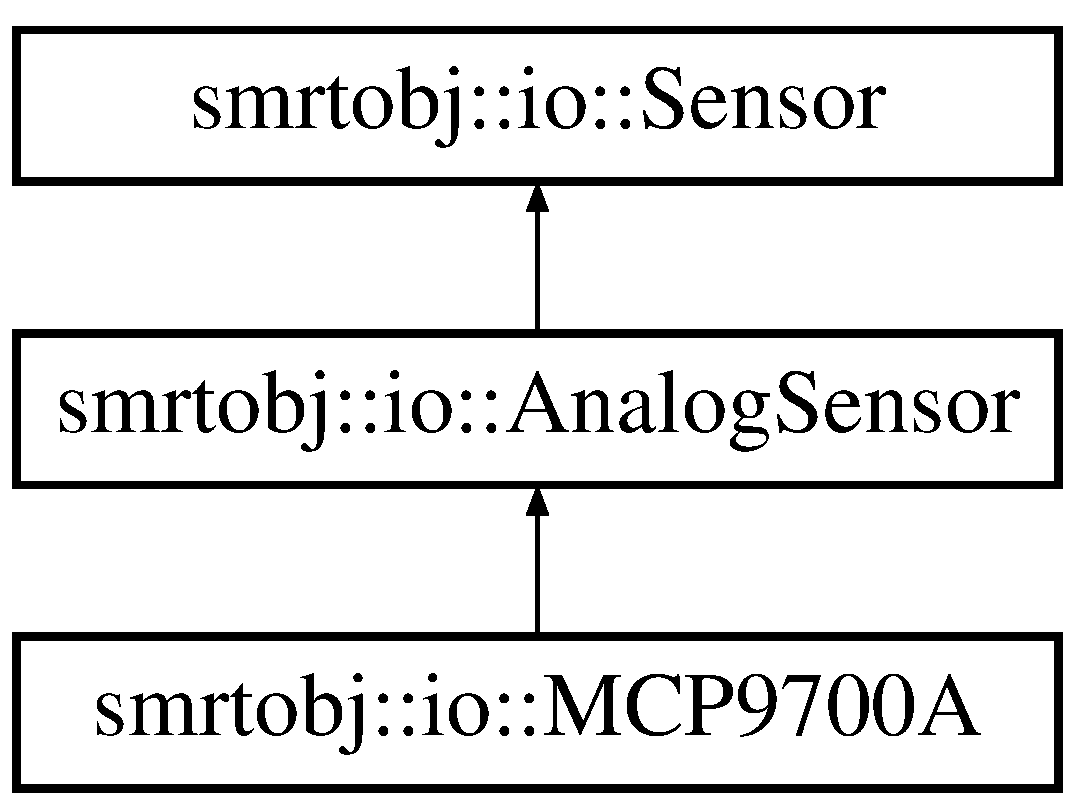
\includegraphics[height=3.000000cm]{classsmrtobj_1_1io_1_1_sensor}
\end{center}
\end{figure}
\subsection*{Public Member Functions}
\begin{DoxyCompactItemize}
\item 
\hyperlink{classsmrtobj_1_1io_1_1_sensor_a342d6d11ef572c8cba92cb76fb1a294b}{Sensor} ()
\item 
\hyperlink{classsmrtobj_1_1io_1_1_sensor_a24ab582f46dbd81e9e7c5b1b94f719bc}{Sensor} (const \hyperlink{classsmrtobj_1_1io_1_1_sensor}{Sensor} \&s)
\item 
virtual \hyperlink{classsmrtobj_1_1io_1_1_sensor_aee8c70e7ef05ce65e7ee33686b5d7db2}{$\sim$\+Sensor} ()
\item 
\hyperlink{classsmrtobj_1_1io_1_1_sensor}{Sensor} \& \hyperlink{classsmrtobj_1_1io_1_1_sensor_aa3297032fa0b0048e497541affd923f2}{operator=} (const \hyperlink{classsmrtobj_1_1io_1_1_sensor}{Sensor} \&s)
\item 
virtual float \hyperlink{classsmrtobj_1_1io_1_1_sensor_aa774a26ce0ca79bf9c76c3cab5336c4b}{measure} ()=0
\end{DoxyCompactItemize}
\subsection*{Static Protected Attributes}
\begin{DoxyCompactItemize}
\item 
\hypertarget{classsmrtobj_1_1io_1_1_sensor_adfb2f64d3363a9bd4d164a4a45fb9829}{}static unsigned long \hyperlink{classsmrtobj_1_1io_1_1_sensor_adfb2f64d3363a9bd4d164a4a45fb9829}{T\+W\+A\+R\+M\+U\+P} = 0\label{classsmrtobj_1_1io_1_1_sensor_adfb2f64d3363a9bd4d164a4a45fb9829}

\begin{DoxyCompactList}\small\item\em Warm up time (in millis). This is the time to wait for having a valid value. \end{DoxyCompactList}\end{DoxyCompactItemize}


\subsection{Detailed Description}
The \hyperlink{classsmrtobj_1_1io_1_1_sensor}{Sensor} class defines the standard interface of a sensor. This is a virtual class and defines a virtual method \char`\"{}measure\char`\"{} to read the sensor. 

Definition at line 21 of file sensor.\+h.



\subsection{Constructor \& Destructor Documentation}
\hypertarget{classsmrtobj_1_1io_1_1_sensor_a342d6d11ef572c8cba92cb76fb1a294b}{}\index{smrtobj\+::io\+::\+Sensor@{smrtobj\+::io\+::\+Sensor}!Sensor@{Sensor}}
\index{Sensor@{Sensor}!smrtobj\+::io\+::\+Sensor@{smrtobj\+::io\+::\+Sensor}}
\subsubsection[{Sensor()}]{\setlength{\rightskip}{0pt plus 5cm}Sensor\+::\+Sensor (
\begin{DoxyParamCaption}
{}
\end{DoxyParamCaption}
)}\label{classsmrtobj_1_1io_1_1_sensor_a342d6d11ef572c8cba92cb76fb1a294b}
Default Constructor. 

Definition at line 18 of file sensor.\+cpp.

\hypertarget{classsmrtobj_1_1io_1_1_sensor_a24ab582f46dbd81e9e7c5b1b94f719bc}{}\index{smrtobj\+::io\+::\+Sensor@{smrtobj\+::io\+::\+Sensor}!Sensor@{Sensor}}
\index{Sensor@{Sensor}!smrtobj\+::io\+::\+Sensor@{smrtobj\+::io\+::\+Sensor}}
\subsubsection[{Sensor(const Sensor \&s)}]{\setlength{\rightskip}{0pt plus 5cm}Sensor\+::\+Sensor (
\begin{DoxyParamCaption}
\item[{const {\bf Sensor} \&}]{s}
\end{DoxyParamCaption}
)}\label{classsmrtobj_1_1io_1_1_sensor_a24ab582f46dbd81e9e7c5b1b94f719bc}
Copy Constructor.


\begin{DoxyParams}[1]{Parameters}
\mbox{\tt in}  & {\em s} & source sensor object \\
\hline
\end{DoxyParams}


Definition at line 24 of file sensor.\+cpp.

\hypertarget{classsmrtobj_1_1io_1_1_sensor_aee8c70e7ef05ce65e7ee33686b5d7db2}{}\index{smrtobj\+::io\+::\+Sensor@{smrtobj\+::io\+::\+Sensor}!````~Sensor@{$\sim$\+Sensor}}
\index{````~Sensor@{$\sim$\+Sensor}!smrtobj\+::io\+::\+Sensor@{smrtobj\+::io\+::\+Sensor}}
\subsubsection[{$\sim$\+Sensor()}]{\setlength{\rightskip}{0pt plus 5cm}Sensor\+::$\sim$\+Sensor (
\begin{DoxyParamCaption}
{}
\end{DoxyParamCaption}
)\hspace{0.3cm}{\ttfamily [virtual]}}\label{classsmrtobj_1_1io_1_1_sensor_aee8c70e7ef05ce65e7ee33686b5d7db2}
Destructor. 

Definition at line 29 of file sensor.\+cpp.



\subsection{Member Function Documentation}
\hypertarget{classsmrtobj_1_1io_1_1_sensor_aa774a26ce0ca79bf9c76c3cab5336c4b}{}\index{smrtobj\+::io\+::\+Sensor@{smrtobj\+::io\+::\+Sensor}!measure@{measure}}
\index{measure@{measure}!smrtobj\+::io\+::\+Sensor@{smrtobj\+::io\+::\+Sensor}}
\subsubsection[{measure()=0}]{\setlength{\rightskip}{0pt plus 5cm}virtual float smrtobj\+::io\+::\+Sensor\+::measure (
\begin{DoxyParamCaption}
{}
\end{DoxyParamCaption}
)\hspace{0.3cm}{\ttfamily [pure virtual]}}\label{classsmrtobj_1_1io_1_1_sensor_aa774a26ce0ca79bf9c76c3cab5336c4b}
Reads sensor and returns the current measurement.

\begin{DoxyReturn}{Returns}
value of the measurement 
\end{DoxyReturn}


Implemented in \hyperlink{classsmrtobj_1_1io_1_1_analog_sensor_a67dd93a15352fa4a98d036194963c4a7}{smrtobj\+::io\+::\+Analog\+Sensor}.

\hypertarget{classsmrtobj_1_1io_1_1_sensor_aa3297032fa0b0048e497541affd923f2}{}\index{smrtobj\+::io\+::\+Sensor@{smrtobj\+::io\+::\+Sensor}!operator=@{operator=}}
\index{operator=@{operator=}!smrtobj\+::io\+::\+Sensor@{smrtobj\+::io\+::\+Sensor}}
\subsubsection[{operator=(const Sensor \&s)}]{\setlength{\rightskip}{0pt plus 5cm}{\bf Sensor} \& Sensor\+::operator= (
\begin{DoxyParamCaption}
\item[{const {\bf Sensor} \&}]{s}
\end{DoxyParamCaption}
)}\label{classsmrtobj_1_1io_1_1_sensor_aa3297032fa0b0048e497541affd923f2}
Override operator =


\begin{DoxyParams}[1]{Parameters}
\mbox{\tt in}  & {\em s} & source sensor object\\
\hline
\end{DoxyParams}
\begin{DoxyReturn}{Returns}
reference of the destination sensor 
\end{DoxyReturn}


Definition at line 34 of file sensor.\+cpp.



The documentation for this class was generated from the following files\+:\begin{DoxyCompactItemize}
\item 
libraries/\+Smrt\+Obj\+I\+O/src/interfaces/\hyperlink{sensor_8h}{sensor.\+h}\item 
libraries/\+Smrt\+Obj\+I\+O/src/interfaces/\hyperlink{sensor_8cpp}{sensor.\+cpp}\end{DoxyCompactItemize}

\hypertarget{classsmrtobj_1_1io_1_1_sensor_temperature}{}\section{smrtobj\+:\+:io\+:\+:Sensor\+Temperature Class Reference}
\label{classsmrtobj_1_1io_1_1_sensor_temperature}\index{smrtobj\+::io\+::\+Sensor\+Temperature@{smrtobj\+::io\+::\+Sensor\+Temperature}}


{\ttfamily \#include $<$sensortemperature.\+h$>$}

Inheritance diagram for smrtobj\+:\+:io\+:\+:Sensor\+Temperature\+:\begin{figure}[H]
\begin{center}
\leavevmode
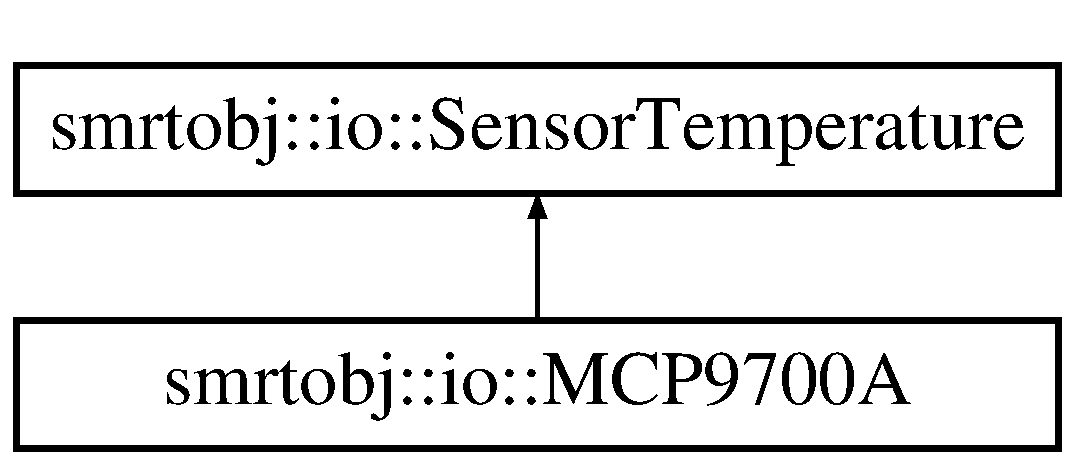
\includegraphics[height=2.000000cm]{classsmrtobj_1_1io_1_1_sensor_temperature}
\end{center}
\end{figure}
\subsection*{Public Member Functions}
\begin{DoxyCompactItemize}
\item 
\hyperlink{classsmrtobj_1_1io_1_1_sensor_temperature_a48b0c65a7f0936a7fc1dd5925755c2b4}{Sensor\+Temperature} ()
\item 
virtual \hyperlink{classsmrtobj_1_1io_1_1_sensor_temperature_a1aee690f03a707a92288aade52571e50}{$\sim$\+Sensor\+Temperature} ()
\item 
virtual float \hyperlink{classsmrtobj_1_1io_1_1_sensor_temperature_abea20003ad3b583d8f7b6021584afabe}{celsius} ()=0
\item 
virtual float \hyperlink{classsmrtobj_1_1io_1_1_sensor_temperature_acd4a57d06be72757c3cdd5f1d14be117}{kelvin} ()=0
\item 
virtual float \hyperlink{classsmrtobj_1_1io_1_1_sensor_temperature_a042ea89c32c26955d03186cc16e049b0}{farenheit} ()=0
\end{DoxyCompactItemize}
\subsection*{Static Public Member Functions}
\begin{DoxyCompactItemize}
\item 
static float \hyperlink{classsmrtobj_1_1io_1_1_sensor_temperature_ae5dc959e4b7594c4391e11422befc1d4}{celsius2farenheit} (float degree)
\item 
static float \hyperlink{classsmrtobj_1_1io_1_1_sensor_temperature_a149aa907b8b6809af604fa26ca4ab195}{farenheit2celsius} (float degree)
\item 
static float \hyperlink{classsmrtobj_1_1io_1_1_sensor_temperature_a3b37e6573c43fa26fd3cf9479e8a58b7}{celsius2kelvin} (float degree)
\item 
static float \hyperlink{classsmrtobj_1_1io_1_1_sensor_temperature_a19f7bc55c7c52aec53c9e28cefa79c42}{kelvin2celsius} (float degree)
\item 
static float \hyperlink{classsmrtobj_1_1io_1_1_sensor_temperature_a14838f9c052b09b64da47c0544975502}{farenheit2kelvin} (float degree)
\item 
static float \hyperlink{classsmrtobj_1_1io_1_1_sensor_temperature_a526a3716f3b1f38ad376bb5c8d3649a4}{kelvin2farenheit} (float degree)
\end{DoxyCompactItemize}


\subsection{Detailed Description}
\hyperlink{classsmrtobj_1_1io_1_1_sensor_temperature}{Sensor\+Temperature} is an interface to model a generic sensor temperature. It defines the main functions to convert the measurement from a unit to an other. The units supported are\+: Celsius, Farenheit and kelvin degrees. 

Definition at line 24 of file sensortemperature.\+h.



\subsection{Constructor \& Destructor Documentation}
\hypertarget{classsmrtobj_1_1io_1_1_sensor_temperature_a48b0c65a7f0936a7fc1dd5925755c2b4}{}\index{smrtobj\+::io\+::\+Sensor\+Temperature@{smrtobj\+::io\+::\+Sensor\+Temperature}!Sensor\+Temperature@{Sensor\+Temperature}}
\index{Sensor\+Temperature@{Sensor\+Temperature}!smrtobj\+::io\+::\+Sensor\+Temperature@{smrtobj\+::io\+::\+Sensor\+Temperature}}
\subsubsection[{Sensor\+Temperature()}]{\setlength{\rightskip}{0pt plus 5cm}smrtobj\+::io\+::\+Sensor\+Temperature\+::\+Sensor\+Temperature (
\begin{DoxyParamCaption}
{}
\end{DoxyParamCaption}
)}\label{classsmrtobj_1_1io_1_1_sensor_temperature_a48b0c65a7f0936a7fc1dd5925755c2b4}
Default Constructor. 

Definition at line 19 of file sensortemperature.\+cpp.

\hypertarget{classsmrtobj_1_1io_1_1_sensor_temperature_a1aee690f03a707a92288aade52571e50}{}\index{smrtobj\+::io\+::\+Sensor\+Temperature@{smrtobj\+::io\+::\+Sensor\+Temperature}!````~Sensor\+Temperature@{$\sim$\+Sensor\+Temperature}}
\index{````~Sensor\+Temperature@{$\sim$\+Sensor\+Temperature}!smrtobj\+::io\+::\+Sensor\+Temperature@{smrtobj\+::io\+::\+Sensor\+Temperature}}
\subsubsection[{$\sim$\+Sensor\+Temperature()}]{\setlength{\rightskip}{0pt plus 5cm}smrtobj\+::io\+::\+Sensor\+Temperature\+::$\sim$\+Sensor\+Temperature (
\begin{DoxyParamCaption}
{}
\end{DoxyParamCaption}
)\hspace{0.3cm}{\ttfamily [virtual]}}\label{classsmrtobj_1_1io_1_1_sensor_temperature_a1aee690f03a707a92288aade52571e50}
Destructor. 

Definition at line 25 of file sensortemperature.\+cpp.



\subsection{Member Function Documentation}
\hypertarget{classsmrtobj_1_1io_1_1_sensor_temperature_abea20003ad3b583d8f7b6021584afabe}{}\index{smrtobj\+::io\+::\+Sensor\+Temperature@{smrtobj\+::io\+::\+Sensor\+Temperature}!celsius@{celsius}}
\index{celsius@{celsius}!smrtobj\+::io\+::\+Sensor\+Temperature@{smrtobj\+::io\+::\+Sensor\+Temperature}}
\subsubsection[{celsius()=0}]{\setlength{\rightskip}{0pt plus 5cm}virtual float smrtobj\+::io\+::\+Sensor\+Temperature\+::celsius (
\begin{DoxyParamCaption}
{}
\end{DoxyParamCaption}
)\hspace{0.3cm}{\ttfamily [pure virtual]}}\label{classsmrtobj_1_1io_1_1_sensor_temperature_abea20003ad3b583d8f7b6021584afabe}
Gets temperature in celsius degrees

\begin{DoxyReturn}{Returns}
celsuius degrees 
\end{DoxyReturn}


Implemented in \hyperlink{classsmrtobj_1_1io_1_1_m_c_p9700_a_ac80d2ee7705df843f6353f579be6f773}{smrtobj\+::io\+::\+M\+C\+P9700\+A}.

\hypertarget{classsmrtobj_1_1io_1_1_sensor_temperature_ae5dc959e4b7594c4391e11422befc1d4}{}\index{smrtobj\+::io\+::\+Sensor\+Temperature@{smrtobj\+::io\+::\+Sensor\+Temperature}!celsius2farenheit@{celsius2farenheit}}
\index{celsius2farenheit@{celsius2farenheit}!smrtobj\+::io\+::\+Sensor\+Temperature@{smrtobj\+::io\+::\+Sensor\+Temperature}}
\subsubsection[{celsius2farenheit(float degree)}]{\setlength{\rightskip}{0pt plus 5cm}float smrtobj\+::io\+::\+Sensor\+Temperature\+::celsius2farenheit (
\begin{DoxyParamCaption}
\item[{float}]{degree}
\end{DoxyParamCaption}
)\hspace{0.3cm}{\ttfamily [static]}}\label{classsmrtobj_1_1io_1_1_sensor_temperature_ae5dc959e4b7594c4391e11422befc1d4}
Converts from celsius to farenheit degrees.


\begin{DoxyParams}[1]{Parameters}
\mbox{\tt in}  & {\em degree} & temperature in celsius degrees\\
\hline
\end{DoxyParams}
\begin{DoxyReturn}{Returns}
farenheit degrees 
\end{DoxyReturn}


Definition at line 30 of file sensortemperature.\+cpp.

\hypertarget{classsmrtobj_1_1io_1_1_sensor_temperature_a3b37e6573c43fa26fd3cf9479e8a58b7}{}\index{smrtobj\+::io\+::\+Sensor\+Temperature@{smrtobj\+::io\+::\+Sensor\+Temperature}!celsius2kelvin@{celsius2kelvin}}
\index{celsius2kelvin@{celsius2kelvin}!smrtobj\+::io\+::\+Sensor\+Temperature@{smrtobj\+::io\+::\+Sensor\+Temperature}}
\subsubsection[{celsius2kelvin(float degree)}]{\setlength{\rightskip}{0pt plus 5cm}float smrtobj\+::io\+::\+Sensor\+Temperature\+::celsius2kelvin (
\begin{DoxyParamCaption}
\item[{float}]{degree}
\end{DoxyParamCaption}
)\hspace{0.3cm}{\ttfamily [static]}}\label{classsmrtobj_1_1io_1_1_sensor_temperature_a3b37e6573c43fa26fd3cf9479e8a58b7}
Converts from celsius to kelvin degrees.


\begin{DoxyParams}[1]{Parameters}
\mbox{\tt in}  & {\em degree} & temperature in celsius degrees\\
\hline
\end{DoxyParams}
\begin{DoxyReturn}{Returns}
kelvin degrees 
\end{DoxyReturn}


Definition at line 49 of file sensortemperature.\+cpp.

\hypertarget{classsmrtobj_1_1io_1_1_sensor_temperature_a042ea89c32c26955d03186cc16e049b0}{}\index{smrtobj\+::io\+::\+Sensor\+Temperature@{smrtobj\+::io\+::\+Sensor\+Temperature}!farenheit@{farenheit}}
\index{farenheit@{farenheit}!smrtobj\+::io\+::\+Sensor\+Temperature@{smrtobj\+::io\+::\+Sensor\+Temperature}}
\subsubsection[{farenheit()=0}]{\setlength{\rightskip}{0pt plus 5cm}virtual float smrtobj\+::io\+::\+Sensor\+Temperature\+::farenheit (
\begin{DoxyParamCaption}
{}
\end{DoxyParamCaption}
)\hspace{0.3cm}{\ttfamily [pure virtual]}}\label{classsmrtobj_1_1io_1_1_sensor_temperature_a042ea89c32c26955d03186cc16e049b0}
Gets temperature in farenheit degrees

\begin{DoxyReturn}{Returns}
farenheit degrees 
\end{DoxyReturn}


Implemented in \hyperlink{classsmrtobj_1_1io_1_1_m_c_p9700_a_a15dc548ff322a4e9f831273d96023038}{smrtobj\+::io\+::\+M\+C\+P9700\+A}.

\hypertarget{classsmrtobj_1_1io_1_1_sensor_temperature_a149aa907b8b6809af604fa26ca4ab195}{}\index{smrtobj\+::io\+::\+Sensor\+Temperature@{smrtobj\+::io\+::\+Sensor\+Temperature}!farenheit2celsius@{farenheit2celsius}}
\index{farenheit2celsius@{farenheit2celsius}!smrtobj\+::io\+::\+Sensor\+Temperature@{smrtobj\+::io\+::\+Sensor\+Temperature}}
\subsubsection[{farenheit2celsius(float degree)}]{\setlength{\rightskip}{0pt plus 5cm}float smrtobj\+::io\+::\+Sensor\+Temperature\+::farenheit2celsius (
\begin{DoxyParamCaption}
\item[{float}]{degree}
\end{DoxyParamCaption}
)\hspace{0.3cm}{\ttfamily [static]}}\label{classsmrtobj_1_1io_1_1_sensor_temperature_a149aa907b8b6809af604fa26ca4ab195}
Converts from farenheit to celsius degrees.


\begin{DoxyParams}[1]{Parameters}
\mbox{\tt in}  & {\em degree} & temperature in farenheit degrees\\
\hline
\end{DoxyParams}
\begin{DoxyReturn}{Returns}
celsius degrees 
\end{DoxyReturn}


Definition at line 39 of file sensortemperature.\+cpp.

\hypertarget{classsmrtobj_1_1io_1_1_sensor_temperature_a14838f9c052b09b64da47c0544975502}{}\index{smrtobj\+::io\+::\+Sensor\+Temperature@{smrtobj\+::io\+::\+Sensor\+Temperature}!farenheit2kelvin@{farenheit2kelvin}}
\index{farenheit2kelvin@{farenheit2kelvin}!smrtobj\+::io\+::\+Sensor\+Temperature@{smrtobj\+::io\+::\+Sensor\+Temperature}}
\subsubsection[{farenheit2kelvin(float degree)}]{\setlength{\rightskip}{0pt plus 5cm}float smrtobj\+::io\+::\+Sensor\+Temperature\+::farenheit2kelvin (
\begin{DoxyParamCaption}
\item[{float}]{degree}
\end{DoxyParamCaption}
)\hspace{0.3cm}{\ttfamily [static]}}\label{classsmrtobj_1_1io_1_1_sensor_temperature_a14838f9c052b09b64da47c0544975502}
Converts from farenheit to kelvin degrees.


\begin{DoxyParams}[1]{Parameters}
\mbox{\tt in}  & {\em degree} & temperature in farenheit degrees\\
\hline
\end{DoxyParams}
\begin{DoxyReturn}{Returns}
kelvin degrees 
\end{DoxyReturn}


Definition at line 63 of file sensortemperature.\+cpp.

\hypertarget{classsmrtobj_1_1io_1_1_sensor_temperature_acd4a57d06be72757c3cdd5f1d14be117}{}\index{smrtobj\+::io\+::\+Sensor\+Temperature@{smrtobj\+::io\+::\+Sensor\+Temperature}!kelvin@{kelvin}}
\index{kelvin@{kelvin}!smrtobj\+::io\+::\+Sensor\+Temperature@{smrtobj\+::io\+::\+Sensor\+Temperature}}
\subsubsection[{kelvin()=0}]{\setlength{\rightskip}{0pt plus 5cm}virtual float smrtobj\+::io\+::\+Sensor\+Temperature\+::kelvin (
\begin{DoxyParamCaption}
{}
\end{DoxyParamCaption}
)\hspace{0.3cm}{\ttfamily [pure virtual]}}\label{classsmrtobj_1_1io_1_1_sensor_temperature_acd4a57d06be72757c3cdd5f1d14be117}
Gets temperature in kelvin degrees

\begin{DoxyReturn}{Returns}
kelvin degrees 
\end{DoxyReturn}


Implemented in \hyperlink{classsmrtobj_1_1io_1_1_m_c_p9700_a_a5ed9f0c208b167fd8e4e1338062d8668}{smrtobj\+::io\+::\+M\+C\+P9700\+A}.

\hypertarget{classsmrtobj_1_1io_1_1_sensor_temperature_a19f7bc55c7c52aec53c9e28cefa79c42}{}\index{smrtobj\+::io\+::\+Sensor\+Temperature@{smrtobj\+::io\+::\+Sensor\+Temperature}!kelvin2celsius@{kelvin2celsius}}
\index{kelvin2celsius@{kelvin2celsius}!smrtobj\+::io\+::\+Sensor\+Temperature@{smrtobj\+::io\+::\+Sensor\+Temperature}}
\subsubsection[{kelvin2celsius(float degree)}]{\setlength{\rightskip}{0pt plus 5cm}float smrtobj\+::io\+::\+Sensor\+Temperature\+::kelvin2celsius (
\begin{DoxyParamCaption}
\item[{float}]{degree}
\end{DoxyParamCaption}
)\hspace{0.3cm}{\ttfamily [static]}}\label{classsmrtobj_1_1io_1_1_sensor_temperature_a19f7bc55c7c52aec53c9e28cefa79c42}
Converts from kelvin to celsius degrees.


\begin{DoxyParams}[1]{Parameters}
\mbox{\tt in}  & {\em degree} & temperature in kelvin degrees\\
\hline
\end{DoxyParams}
\begin{DoxyReturn}{Returns}
celsius degrees 
\end{DoxyReturn}


Definition at line 56 of file sensortemperature.\+cpp.

\hypertarget{classsmrtobj_1_1io_1_1_sensor_temperature_a526a3716f3b1f38ad376bb5c8d3649a4}{}\index{smrtobj\+::io\+::\+Sensor\+Temperature@{smrtobj\+::io\+::\+Sensor\+Temperature}!kelvin2farenheit@{kelvin2farenheit}}
\index{kelvin2farenheit@{kelvin2farenheit}!smrtobj\+::io\+::\+Sensor\+Temperature@{smrtobj\+::io\+::\+Sensor\+Temperature}}
\subsubsection[{kelvin2farenheit(float degree)}]{\setlength{\rightskip}{0pt plus 5cm}float smrtobj\+::io\+::\+Sensor\+Temperature\+::kelvin2farenheit (
\begin{DoxyParamCaption}
\item[{float}]{degree}
\end{DoxyParamCaption}
)\hspace{0.3cm}{\ttfamily [static]}}\label{classsmrtobj_1_1io_1_1_sensor_temperature_a526a3716f3b1f38ad376bb5c8d3649a4}
Converts from kelvin to farenheit degrees.


\begin{DoxyParams}[1]{Parameters}
\mbox{\tt in}  & {\em degree} & temperature in kelvin degrees\\
\hline
\end{DoxyParams}
\begin{DoxyReturn}{Returns}
farenheit degrees 
\end{DoxyReturn}


Definition at line 69 of file sensortemperature.\+cpp.



The documentation for this class was generated from the following files\+:\begin{DoxyCompactItemize}
\item 
libraries/\+Smrt\+Obj\+I\+O/src/interfaces/\hyperlink{sensortemperature_8h}{sensortemperature.\+h}\item 
libraries/\+Smrt\+Obj\+I\+O/src/interfaces/sensortemperature.\+cpp\end{DoxyCompactItemize}

\hypertarget{classsmrtobj_1_1io_1_1_signal}{}\section{smrtobj\+:\+:io\+:\+:Signal Class Reference}
\label{classsmrtobj_1_1io_1_1_signal}\index{smrtobj\+::io\+::\+Signal@{smrtobj\+::io\+::\+Signal}}


{\ttfamily \#include $<$signal.\+h$>$}

Inheritance diagram for smrtobj\+:\+:io\+:\+:Signal\+:\begin{figure}[H]
\begin{center}
\leavevmode
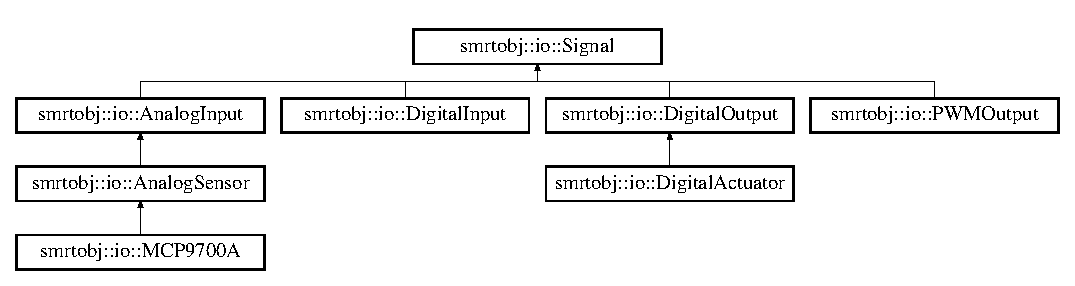
\includegraphics[height=3.393939cm]{classsmrtobj_1_1io_1_1_signal}
\end{center}
\end{figure}
\subsection*{Public Types}
\begin{DoxyCompactItemize}
\item 
enum \hyperlink{classsmrtobj_1_1io_1_1_signal_a0566106724452894eae48ec38b66952c}{\+\_\+type} \{ \hyperlink{classsmrtobj_1_1io_1_1_signal_a0566106724452894eae48ec38b66952ca8c9957bb35f431c7299566ecd15b0091}{N\+O\+T\+\_\+\+I\+N\+I\+T\+I\+A\+L\+I\+Z\+E\+D} = 0x00, 
\hyperlink{classsmrtobj_1_1io_1_1_signal_a0566106724452894eae48ec38b66952caccc24da2e76e4a69c273fbfdfa6d059a}{T\+Y\+P\+E\+\_\+\+I\+N\+P\+U\+T} = 0x01, 
\hyperlink{classsmrtobj_1_1io_1_1_signal_a0566106724452894eae48ec38b66952ca1cd32fb0f22887a6df6296f849d035ff}{T\+Y\+P\+E\+\_\+\+O\+U\+T\+P\+U\+T} = 0x02, 
\hyperlink{classsmrtobj_1_1io_1_1_signal_a0566106724452894eae48ec38b66952caf8a436cfbf1fd32224a08b8fbff821a9}{T\+Y\+P\+E\+\_\+\+B\+I\+D\+I\+R\+E\+C\+T\+I\+O\+N\+A\+L} = 0x03
 \}
\end{DoxyCompactItemize}
\subsection*{Public Member Functions}
\begin{DoxyCompactItemize}
\item 
\hyperlink{classsmrtobj_1_1io_1_1_signal_a7e69e538253d90c3f551f4701a1f94a5}{Signal} ()
\item 
\hyperlink{classsmrtobj_1_1io_1_1_signal_a0482d58a322aeb3be54aa446442f0663}{Signal} (const \hyperlink{classsmrtobj_1_1io_1_1_signal}{Signal} \&s)
\item 
virtual \hyperlink{classsmrtobj_1_1io_1_1_signal_ae7a1d116cda63e790bf9aab549d57d3a}{$\sim$\+Signal} ()
\item 
\hyperlink{classsmrtobj_1_1io_1_1_signal}{Signal} \& \hyperlink{classsmrtobj_1_1io_1_1_signal_a749ffe1ea8adb870aa211f346de35e08}{operator=} (const \hyperlink{classsmrtobj_1_1io_1_1_signal}{Signal} \&s)
\item 
virtual byte \hyperlink{classsmrtobj_1_1io_1_1_signal_a38cd36f413f1ad2213684e4364ac4270}{type} ()=0
\item 
bool \hyperlink{classsmrtobj_1_1io_1_1_signal_a6486ccfa94b91c8596e6f11f61736844}{is\+Open} ()
\end{DoxyCompactItemize}
\subsection*{Protected Attributes}
\begin{DoxyCompactItemize}
\item 
\hypertarget{classsmrtobj_1_1io_1_1_signal_acb7bac283b07ef39ec419a83b98df929}{}byte \hyperlink{classsmrtobj_1_1io_1_1_signal_acb7bac283b07ef39ec419a83b98df929}{m\+\_\+type}\label{classsmrtobj_1_1io_1_1_signal_acb7bac283b07ef39ec419a83b98df929}

\begin{DoxyCompactList}\small\item\em \hyperlink{classsmrtobj_1_1io_1_1_signal}{Signal} interface type. \end{DoxyCompactList}\item 
\hypertarget{classsmrtobj_1_1io_1_1_signal_a2f7993ca7fcf743c5ce6bc4d69444c93}{}bool \hyperlink{classsmrtobj_1_1io_1_1_signal_a2f7993ca7fcf743c5ce6bc4d69444c93}{m\+\_\+open}\label{classsmrtobj_1_1io_1_1_signal_a2f7993ca7fcf743c5ce6bc4d69444c93}

\begin{DoxyCompactList}\small\item\em false if the interface is not initialized yet, true otherwise \end{DoxyCompactList}\end{DoxyCompactItemize}


\subsection{Detailed Description}
\hyperlink{classsmrtobj_1_1io_1_1_signal}{Signal} is an abstract class to model an interface for every I/\+O signal of an Arduino board. It is possible define the type of signal (Input or Output).

{\bfseries T\+Y\+P\+E\+\_\+\+I\+N\+P\+U\+T} Arduino (Atmega) pins configured as I\+N\+P\+U\+T with pin\+Mode() are said to be in a high-\/impedance state. Pins configured as I\+N\+P\+U\+T make extremely small demands on the circuit that they are sampling, equivalent to a series resistor of 100 Megohms in front of the pin. This makes them useful for reading a sensor.

{\bfseries T\+Y\+P\+E\+\_\+\+O\+U\+T\+P\+U\+T} Pins configured as O\+U\+T\+P\+U\+T are said to be in a low-\/impedance state. This means that they can provide a substantial amount of current to other circuits. Atmega pins can source (provide current) or sink (absorb current) up to 40 m\+A (milliamps) of current to other devices/circuits. This makes them useful for powering L\+E\+Ds because L\+E\+Ds typically use less than 40 m\+A. Loads greater than 40 m\+A (e.\+g. motors) will require a transistor or other interface circuitry.~\newline
Pins configured as outputs can be damaged or destroyed if they are connected to either the ground or positive power rails. 

Definition at line 43 of file signal.\+h.



\subsection{Member Enumeration Documentation}
\hypertarget{classsmrtobj_1_1io_1_1_signal_a0566106724452894eae48ec38b66952c}{}\index{smrtobj\+::io\+::\+Signal@{smrtobj\+::io\+::\+Signal}!\+\_\+type@{\+\_\+type}}
\index{\+\_\+type@{\+\_\+type}!smrtobj\+::io\+::\+Signal@{smrtobj\+::io\+::\+Signal}}
\subsubsection[{\+\_\+type}]{\setlength{\rightskip}{0pt plus 5cm}enum {\bf smrtobj\+::io\+::\+Signal\+::\+\_\+type}}\label{classsmrtobj_1_1io_1_1_signal_a0566106724452894eae48ec38b66952c}
Type of signal \begin{Desc}
\item[Enumerator]\par
\begin{description}
\index{N\+O\+T\+\_\+\+I\+N\+I\+T\+I\+A\+L\+I\+Z\+E\+D@{N\+O\+T\+\_\+\+I\+N\+I\+T\+I\+A\+L\+I\+Z\+E\+D}!smrtobj\+::io\+::\+Signal@{smrtobj\+::io\+::\+Signal}}\index{smrtobj\+::io\+::\+Signal@{smrtobj\+::io\+::\+Signal}!N\+O\+T\+\_\+\+I\+N\+I\+T\+I\+A\+L\+I\+Z\+E\+D@{N\+O\+T\+\_\+\+I\+N\+I\+T\+I\+A\+L\+I\+Z\+E\+D}}\item[{\em 
\hypertarget{classsmrtobj_1_1io_1_1_signal_a0566106724452894eae48ec38b66952ca8c9957bb35f431c7299566ecd15b0091}{}N\+O\+T\+\_\+\+I\+N\+I\+T\+I\+A\+L\+I\+Z\+E\+D\label{classsmrtobj_1_1io_1_1_signal_a0566106724452894eae48ec38b66952ca8c9957bb35f431c7299566ecd15b0091}
}]Not initialized. \index{T\+Y\+P\+E\+\_\+\+I\+N\+P\+U\+T@{T\+Y\+P\+E\+\_\+\+I\+N\+P\+U\+T}!smrtobj\+::io\+::\+Signal@{smrtobj\+::io\+::\+Signal}}\index{smrtobj\+::io\+::\+Signal@{smrtobj\+::io\+::\+Signal}!T\+Y\+P\+E\+\_\+\+I\+N\+P\+U\+T@{T\+Y\+P\+E\+\_\+\+I\+N\+P\+U\+T}}\item[{\em 
\hypertarget{classsmrtobj_1_1io_1_1_signal_a0566106724452894eae48ec38b66952caccc24da2e76e4a69c273fbfdfa6d059a}{}T\+Y\+P\+E\+\_\+\+I\+N\+P\+U\+T\label{classsmrtobj_1_1io_1_1_signal_a0566106724452894eae48ec38b66952caccc24da2e76e4a69c273fbfdfa6d059a}
}]Input. \index{T\+Y\+P\+E\+\_\+\+O\+U\+T\+P\+U\+T@{T\+Y\+P\+E\+\_\+\+O\+U\+T\+P\+U\+T}!smrtobj\+::io\+::\+Signal@{smrtobj\+::io\+::\+Signal}}\index{smrtobj\+::io\+::\+Signal@{smrtobj\+::io\+::\+Signal}!T\+Y\+P\+E\+\_\+\+O\+U\+T\+P\+U\+T@{T\+Y\+P\+E\+\_\+\+O\+U\+T\+P\+U\+T}}\item[{\em 
\hypertarget{classsmrtobj_1_1io_1_1_signal_a0566106724452894eae48ec38b66952ca1cd32fb0f22887a6df6296f849d035ff}{}T\+Y\+P\+E\+\_\+\+O\+U\+T\+P\+U\+T\label{classsmrtobj_1_1io_1_1_signal_a0566106724452894eae48ec38b66952ca1cd32fb0f22887a6df6296f849d035ff}
}]Output. \index{T\+Y\+P\+E\+\_\+\+B\+I\+D\+I\+R\+E\+C\+T\+I\+O\+N\+A\+L@{T\+Y\+P\+E\+\_\+\+B\+I\+D\+I\+R\+E\+C\+T\+I\+O\+N\+A\+L}!smrtobj\+::io\+::\+Signal@{smrtobj\+::io\+::\+Signal}}\index{smrtobj\+::io\+::\+Signal@{smrtobj\+::io\+::\+Signal}!T\+Y\+P\+E\+\_\+\+B\+I\+D\+I\+R\+E\+C\+T\+I\+O\+N\+A\+L@{T\+Y\+P\+E\+\_\+\+B\+I\+D\+I\+R\+E\+C\+T\+I\+O\+N\+A\+L}}\item[{\em 
\hypertarget{classsmrtobj_1_1io_1_1_signal_a0566106724452894eae48ec38b66952caf8a436cfbf1fd32224a08b8fbff821a9}{}T\+Y\+P\+E\+\_\+\+B\+I\+D\+I\+R\+E\+C\+T\+I\+O\+N\+A\+L\label{classsmrtobj_1_1io_1_1_signal_a0566106724452894eae48ec38b66952caf8a436cfbf1fd32224a08b8fbff821a9}
}]bidirectional \end{description}
\end{Desc}


Definition at line 51 of file signal.\+h.



\subsection{Constructor \& Destructor Documentation}
\hypertarget{classsmrtobj_1_1io_1_1_signal_a7e69e538253d90c3f551f4701a1f94a5}{}\index{smrtobj\+::io\+::\+Signal@{smrtobj\+::io\+::\+Signal}!Signal@{Signal}}
\index{Signal@{Signal}!smrtobj\+::io\+::\+Signal@{smrtobj\+::io\+::\+Signal}}
\subsubsection[{Signal()}]{\setlength{\rightskip}{0pt plus 5cm}Signal\+::\+Signal (
\begin{DoxyParamCaption}
{}
\end{DoxyParamCaption}
)}\label{classsmrtobj_1_1io_1_1_signal_a7e69e538253d90c3f551f4701a1f94a5}
Default Constructor. It initializes all attribute of the signal interface\+: type will be not initialized and state will be not opened yet. 

Definition at line 16 of file signal.\+cpp.

\hypertarget{classsmrtobj_1_1io_1_1_signal_a0482d58a322aeb3be54aa446442f0663}{}\index{smrtobj\+::io\+::\+Signal@{smrtobj\+::io\+::\+Signal}!Signal@{Signal}}
\index{Signal@{Signal}!smrtobj\+::io\+::\+Signal@{smrtobj\+::io\+::\+Signal}}
\subsubsection[{Signal(const Signal \&s)}]{\setlength{\rightskip}{0pt plus 5cm}Signal\+::\+Signal (
\begin{DoxyParamCaption}
\item[{const {\bf Signal} \&}]{s}
\end{DoxyParamCaption}
)}\label{classsmrtobj_1_1io_1_1_signal_a0482d58a322aeb3be54aa446442f0663}
Copy Constructor.


\begin{DoxyParams}[1]{Parameters}
\mbox{\tt in}  & {\em s} & source signal object \\
\hline
\end{DoxyParams}


Definition at line 20 of file signal.\+cpp.

\hypertarget{classsmrtobj_1_1io_1_1_signal_ae7a1d116cda63e790bf9aab549d57d3a}{}\index{smrtobj\+::io\+::\+Signal@{smrtobj\+::io\+::\+Signal}!````~Signal@{$\sim$\+Signal}}
\index{````~Signal@{$\sim$\+Signal}!smrtobj\+::io\+::\+Signal@{smrtobj\+::io\+::\+Signal}}
\subsubsection[{$\sim$\+Signal()}]{\setlength{\rightskip}{0pt plus 5cm}Signal\+::$\sim$\+Signal (
\begin{DoxyParamCaption}
{}
\end{DoxyParamCaption}
)\hspace{0.3cm}{\ttfamily [virtual]}}\label{classsmrtobj_1_1io_1_1_signal_ae7a1d116cda63e790bf9aab549d57d3a}
Destructor. 

Definition at line 26 of file signal.\+cpp.



\subsection{Member Function Documentation}
\hypertarget{classsmrtobj_1_1io_1_1_signal_a6486ccfa94b91c8596e6f11f61736844}{}\index{smrtobj\+::io\+::\+Signal@{smrtobj\+::io\+::\+Signal}!is\+Open@{is\+Open}}
\index{is\+Open@{is\+Open}!smrtobj\+::io\+::\+Signal@{smrtobj\+::io\+::\+Signal}}
\subsubsection[{is\+Open()}]{\setlength{\rightskip}{0pt plus 5cm}bool smrtobj\+::io\+::\+Signal\+::is\+Open (
\begin{DoxyParamCaption}
{}
\end{DoxyParamCaption}
)\hspace{0.3cm}{\ttfamily [inline]}}\label{classsmrtobj_1_1io_1_1_signal_a6486ccfa94b91c8596e6f11f61736844}
Checks if the interface is open or not

\begin{DoxyReturn}{Returns}
false if the interface is not initialized yet, true otherwise 
\end{DoxyReturn}


Definition at line 110 of file signal.\+h.

\hypertarget{classsmrtobj_1_1io_1_1_signal_a749ffe1ea8adb870aa211f346de35e08}{}\index{smrtobj\+::io\+::\+Signal@{smrtobj\+::io\+::\+Signal}!operator=@{operator=}}
\index{operator=@{operator=}!smrtobj\+::io\+::\+Signal@{smrtobj\+::io\+::\+Signal}}
\subsubsection[{operator=(const Signal \&s)}]{\setlength{\rightskip}{0pt plus 5cm}{\bf Signal} \& Signal\+::operator= (
\begin{DoxyParamCaption}
\item[{const {\bf Signal} \&}]{s}
\end{DoxyParamCaption}
)}\label{classsmrtobj_1_1io_1_1_signal_a749ffe1ea8adb870aa211f346de35e08}
Override operator =


\begin{DoxyParams}[1]{Parameters}
\mbox{\tt in}  & {\em s} & source signal object\\
\hline
\end{DoxyParams}
\begin{DoxyReturn}{Returns}
destination signal reference 
\end{DoxyReturn}


Definition at line 30 of file signal.\+cpp.

\hypertarget{classsmrtobj_1_1io_1_1_signal_a38cd36f413f1ad2213684e4364ac4270}{}\index{smrtobj\+::io\+::\+Signal@{smrtobj\+::io\+::\+Signal}!type@{type}}
\index{type@{type}!smrtobj\+::io\+::\+Signal@{smrtobj\+::io\+::\+Signal}}
\subsubsection[{type()=0}]{\setlength{\rightskip}{0pt plus 5cm}virtual byte smrtobj\+::io\+::\+Signal\+::type (
\begin{DoxyParamCaption}
{}
\end{DoxyParamCaption}
)\hspace{0.3cm}{\ttfamily [pure virtual]}}\label{classsmrtobj_1_1io_1_1_signal_a38cd36f413f1ad2213684e4364ac4270}
Virtual method, it gets the type of the interface according to \hyperlink{classsmrtobj_1_1io_1_1_signal_a0566106724452894eae48ec38b66952c}{smrtobj\+::io\+::\+Signal\+::\+\_\+type} enum

\begin{DoxyReturn}{Returns}
the type of the signal interface 
\end{DoxyReturn}


Implemented in \hyperlink{classsmrtobj_1_1io_1_1_analog_input_a08fe1be7aca445768e1b2293cb48b96a}{smrtobj\+::io\+::\+Analog\+Input}, \hyperlink{classsmrtobj_1_1io_1_1_digital_input_a89f92208f29c7ca20cdc35689c8aad6a}{smrtobj\+::io\+::\+Digital\+Input}, \hyperlink{classsmrtobj_1_1io_1_1_p_w_m_output_ac5908c2317a1e2e7a293f8ee04d42a77}{smrtobj\+::io\+::\+P\+W\+M\+Output}, and \hyperlink{classsmrtobj_1_1io_1_1_digital_output_a9c9e665bb38c2c8164cfce1a3ce94dcc}{smrtobj\+::io\+::\+Digital\+Output}.



The documentation for this class was generated from the following files\+:\begin{DoxyCompactItemize}
\item 
libraries/\+Smrt\+Obj\+I\+O/src/interfaces/\hyperlink{signal_8h}{signal.\+h}\item 
libraries/\+Smrt\+Obj\+I\+O/src/interfaces/\hyperlink{signal_8cpp}{signal.\+cpp}\end{DoxyCompactItemize}

\hypertarget{classsmrtobj_1_1parser_1_1_string_parser}{}\section{smrtobj\+:\+:parser\+:\+:String\+Parser Class Reference}
\label{classsmrtobj_1_1parser_1_1_string_parser}\index{smrtobj\+::parser\+::\+String\+Parser@{smrtobj\+::parser\+::\+String\+Parser}}


{\ttfamily \#include $<$stringparser.\+h$>$}

\subsection*{Public Member Functions}
\begin{DoxyCompactItemize}
\item 
\hyperlink{classsmrtobj_1_1parser_1_1_string_parser_a855c13686d232d10fc7264fb4e13a2fb}{String\+Parser} ()
\item 
virtual \hyperlink{classsmrtobj_1_1parser_1_1_string_parser_ac62234192a7e3fa3041d0838f31b5d01}{$\sim$\+String\+Parser} ()
\end{DoxyCompactItemize}
\subsection*{Static Public Member Functions}
\begin{DoxyCompactItemize}
\item 
static bool \hyperlink{classsmrtobj_1_1parser_1_1_string_parser_a286ba7afb015d6101dce638ca639980e}{to\+Int} (char $\ast$str, uint8\+\_\+t \&n, uint8\+\_\+t size=255)
\item 
static bool \hyperlink{classsmrtobj_1_1parser_1_1_string_parser_a238387a4fcadf8f9e5eb84d52e46d054}{to\+Int} (char $\ast$str, int \&n, uint8\+\_\+t size=255)
\item 
static bool \hyperlink{classsmrtobj_1_1parser_1_1_string_parser_a60d66796fdacb1b3a93603d48ce81c6b}{to\+Int} (char $\ast$str, unsigned int \&n, uint8\+\_\+t size)
\item 
static bool \hyperlink{classsmrtobj_1_1parser_1_1_string_parser_ad2dd013347a1bb807549e3aa1ec1bff6}{to\+Long} (char $\ast$str, long \&n, uint8\+\_\+t size)
\item 
static bool \hyperlink{classsmrtobj_1_1parser_1_1_string_parser_a8545f1404542abfac2ccb15675ed4891}{to\+Long} (char $\ast$str, unsigned long \&n, uint8\+\_\+t size)
\item 
static bool \hyperlink{classsmrtobj_1_1parser_1_1_string_parser_a8e36c1d12527b4120cbde1bbbdc18562}{to\+Float} (char $\ast$str, float \&n, uint8\+\_\+t size)
\item 
static bool \hyperlink{classsmrtobj_1_1parser_1_1_string_parser_a35408e896e31a3de9271f4950d8ed891}{to\+I\+P\+Address} (char $\ast$str, uint8\+\_\+t $\ast$ip, uint8\+\_\+t size=255)
\item 
static bool \hyperlink{classsmrtobj_1_1parser_1_1_string_parser_a454373fb32886498a684d49b49897474}{is\+Digit\+Str} (char $\ast$str, uint8\+\_\+t size=255)
\item 
static bool \hyperlink{classsmrtobj_1_1parser_1_1_string_parser_a7584c8c2b0859c1160cb4fc1ece14e2d}{is\+I\+P\+Address} (char $\ast$str, uint8\+\_\+t size=255)
\item 
static bool \hyperlink{classsmrtobj_1_1parser_1_1_string_parser_a2dc94649a00e706b4ce7d62cc6d6fd11}{is\+Float\+Str} (char $\ast$str, uint8\+\_\+t size=255)
\item 
static bool \hyperlink{classsmrtobj_1_1parser_1_1_string_parser_aeafed5972a553a95c9a1cd0b6f77f771}{convert\+Float} (float n, char $\ast$buff, uint8\+\_\+t stot, uint8\+\_\+t decimal)
\item 
static bool \hyperlink{classsmrtobj_1_1parser_1_1_string_parser_a532a1adbdd310bb30f64a26565f0cb77}{read\+String\+From\+Flash} (const char str\mbox{[}$\,$\mbox{]} P\+R\+O\+G\+M\+E\+M, char $\ast$buf, uint8\+\_\+t size\+\_\+b)
\end{DoxyCompactItemize}


\subsection{Detailed Description}
\hyperlink{classsmrtobj_1_1parser_1_1_string_parser}{String\+Parser} is a collection of functions to parse and use strings. 

Definition at line 30 of file stringparser.\+h.



\subsection{Constructor \& Destructor Documentation}
\hypertarget{classsmrtobj_1_1parser_1_1_string_parser_a855c13686d232d10fc7264fb4e13a2fb}{}\index{smrtobj\+::parser\+::\+String\+Parser@{smrtobj\+::parser\+::\+String\+Parser}!String\+Parser@{String\+Parser}}
\index{String\+Parser@{String\+Parser}!smrtobj\+::parser\+::\+String\+Parser@{smrtobj\+::parser\+::\+String\+Parser}}
\subsubsection[{String\+Parser()}]{\setlength{\rightskip}{0pt plus 5cm}smrtobj\+::i2c\+::\+String\+Parser\+::\+String\+Parser (
\begin{DoxyParamCaption}
{}
\end{DoxyParamCaption}
)}\label{classsmrtobj_1_1parser_1_1_string_parser_a855c13686d232d10fc7264fb4e13a2fb}
Default Constructor It sets all internal variables as the start time at current time as seconds from 1970. 

Definition at line 17 of file stringparser.\+cpp.

\hypertarget{classsmrtobj_1_1parser_1_1_string_parser_ac62234192a7e3fa3041d0838f31b5d01}{}\index{smrtobj\+::parser\+::\+String\+Parser@{smrtobj\+::parser\+::\+String\+Parser}!````~String\+Parser@{$\sim$\+String\+Parser}}
\index{````~String\+Parser@{$\sim$\+String\+Parser}!smrtobj\+::parser\+::\+String\+Parser@{smrtobj\+::parser\+::\+String\+Parser}}
\subsubsection[{$\sim$\+String\+Parser()}]{\setlength{\rightskip}{0pt plus 5cm}smrtobj\+::i2c\+::\+String\+Parser\+::$\sim$\+String\+Parser (
\begin{DoxyParamCaption}
{}
\end{DoxyParamCaption}
)\hspace{0.3cm}{\ttfamily [virtual]}}\label{classsmrtobj_1_1parser_1_1_string_parser_ac62234192a7e3fa3041d0838f31b5d01}
Destructor 

Definition at line 21 of file stringparser.\+cpp.



\subsection{Member Function Documentation}
\hypertarget{classsmrtobj_1_1parser_1_1_string_parser_aeafed5972a553a95c9a1cd0b6f77f771}{}\index{smrtobj\+::parser\+::\+String\+Parser@{smrtobj\+::parser\+::\+String\+Parser}!convert\+Float@{convert\+Float}}
\index{convert\+Float@{convert\+Float}!smrtobj\+::parser\+::\+String\+Parser@{smrtobj\+::parser\+::\+String\+Parser}}
\subsubsection[{convert\+Float(float n, char $\ast$buff, uint8\+\_\+t stot, uint8\+\_\+t decimal)}]{\setlength{\rightskip}{0pt plus 5cm}bool smrtobj\+::i2c\+::\+String\+Parser\+::convert\+Float (
\begin{DoxyParamCaption}
\item[{float}]{n, }
\item[{char $\ast$}]{buff, }
\item[{uint8\+\_\+t}]{stot, }
\item[{uint8\+\_\+t}]{decimal}
\end{DoxyParamCaption}
)\hspace{0.3cm}{\ttfamily [static]}}\label{classsmrtobj_1_1parser_1_1_string_parser_aeafed5972a553a95c9a1cd0b6f77f771}
Converts a floating number to a string of maximum size stot and save it in str. The number of decimals are set by the parameter decimal.


\begin{DoxyParams}[1]{Parameters}
\mbox{\tt in}  & {\em n} & number to convert in a string. \\
\hline
\mbox{\tt in}  & {\em buff} & where store the number as a string. \\
\hline
\mbox{\tt in}  & {\em stot} & maximim size of the string. \\
\hline
\mbox{\tt in}  & {\em decimal} & number of decimals.\\
\hline
\end{DoxyParams}
\begin{DoxyReturn}{Returns}
false if the strins is not enough big. 
\end{DoxyReturn}


Definition at line 261 of file stringparser.\+cpp.

\hypertarget{classsmrtobj_1_1parser_1_1_string_parser_a454373fb32886498a684d49b49897474}{}\index{smrtobj\+::parser\+::\+String\+Parser@{smrtobj\+::parser\+::\+String\+Parser}!is\+Digit\+Str@{is\+Digit\+Str}}
\index{is\+Digit\+Str@{is\+Digit\+Str}!smrtobj\+::parser\+::\+String\+Parser@{smrtobj\+::parser\+::\+String\+Parser}}
\subsubsection[{is\+Digit\+Str(char $\ast$str, uint8\+\_\+t size=255)}]{\setlength{\rightskip}{0pt plus 5cm}bool smrtobj\+::i2c\+::\+String\+Parser\+::is\+Digit\+Str (
\begin{DoxyParamCaption}
\item[{char $\ast$}]{str, }
\item[{uint8\+\_\+t}]{size = {\ttfamily 255}}
\end{DoxyParamCaption}
)\hspace{0.3cm}{\ttfamily [static]}}\label{classsmrtobj_1_1parser_1_1_string_parser_a454373fb32886498a684d49b49897474}
Checks if the string str contains an integer number. It returns false if the string is not an integer number.


\begin{DoxyParams}[1]{Parameters}
\mbox{\tt in}  & {\em str} & string with the representation of an integer number. \\
\hline
\mbox{\tt in}  & {\em size} & maximum size of string str.\\
\hline
\end{DoxyParams}
\begin{DoxyReturn}{Returns}
false if the string is not an integer number. 
\end{DoxyReturn}


Definition at line 25 of file stringparser.\+cpp.

\hypertarget{classsmrtobj_1_1parser_1_1_string_parser_a2dc94649a00e706b4ce7d62cc6d6fd11}{}\index{smrtobj\+::parser\+::\+String\+Parser@{smrtobj\+::parser\+::\+String\+Parser}!is\+Float\+Str@{is\+Float\+Str}}
\index{is\+Float\+Str@{is\+Float\+Str}!smrtobj\+::parser\+::\+String\+Parser@{smrtobj\+::parser\+::\+String\+Parser}}
\subsubsection[{is\+Float\+Str(char $\ast$str, uint8\+\_\+t size=255)}]{\setlength{\rightskip}{0pt plus 5cm}bool smrtobj\+::i2c\+::\+String\+Parser\+::is\+Float\+Str (
\begin{DoxyParamCaption}
\item[{char $\ast$}]{str, }
\item[{uint8\+\_\+t}]{size = {\ttfamily 255}}
\end{DoxyParamCaption}
)\hspace{0.3cm}{\ttfamily [static]}}\label{classsmrtobj_1_1parser_1_1_string_parser_a2dc94649a00e706b4ce7d62cc6d6fd11}
Checks if the string str contains a floating point number. It returns false if the string is not a floating point numbers.


\begin{DoxyParams}[1]{Parameters}
\mbox{\tt in}  & {\em str} & string with the representation of a floating point number. \\
\hline
\mbox{\tt in}  & {\em size} & maximum size of string str.\\
\hline
\end{DoxyParams}
\begin{DoxyReturn}{Returns}
false if the string is not a floating point numbers. 
\end{DoxyReturn}


Definition at line 112 of file stringparser.\+cpp.

\hypertarget{classsmrtobj_1_1parser_1_1_string_parser_a7584c8c2b0859c1160cb4fc1ece14e2d}{}\index{smrtobj\+::parser\+::\+String\+Parser@{smrtobj\+::parser\+::\+String\+Parser}!is\+I\+P\+Address@{is\+I\+P\+Address}}
\index{is\+I\+P\+Address@{is\+I\+P\+Address}!smrtobj\+::parser\+::\+String\+Parser@{smrtobj\+::parser\+::\+String\+Parser}}
\subsubsection[{is\+I\+P\+Address(char $\ast$str, uint8\+\_\+t size=255)}]{\setlength{\rightskip}{0pt plus 5cm}bool smrtobj\+::i2c\+::\+String\+Parser\+::is\+I\+P\+Address (
\begin{DoxyParamCaption}
\item[{char $\ast$}]{str, }
\item[{uint8\+\_\+t}]{size = {\ttfamily 255}}
\end{DoxyParamCaption}
)\hspace{0.3cm}{\ttfamily [static]}}\label{classsmrtobj_1_1parser_1_1_string_parser_a7584c8c2b0859c1160cb4fc1ece14e2d}
Checks if the string str contains an I\+P address. It returns false if the string is not an I\+P address.


\begin{DoxyParams}[1]{Parameters}
\mbox{\tt in}  & {\em str} & string with the representation of an I\+P address. \\
\hline
\mbox{\tt in}  & {\em size} & maximum size of string str.\\
\hline
\end{DoxyParams}
\begin{DoxyReturn}{Returns}
false if the string is not an I\+P address. 
\end{DoxyReturn}


Definition at line 45 of file stringparser.\+cpp.

\hypertarget{classsmrtobj_1_1parser_1_1_string_parser_a532a1adbdd310bb30f64a26565f0cb77}{}\index{smrtobj\+::parser\+::\+String\+Parser@{smrtobj\+::parser\+::\+String\+Parser}!read\+String\+From\+Flash@{read\+String\+From\+Flash}}
\index{read\+String\+From\+Flash@{read\+String\+From\+Flash}!smrtobj\+::parser\+::\+String\+Parser@{smrtobj\+::parser\+::\+String\+Parser}}
\subsubsection[{read\+String\+From\+Flash(const char str[] P\+R\+O\+G\+M\+E\+M, char $\ast$buf, uint8\+\_\+t size\+\_\+b)}]{\setlength{\rightskip}{0pt plus 5cm}bool smrtobj\+::i2c\+::\+String\+Parser\+::read\+String\+From\+Flash (
\begin{DoxyParamCaption}
\item[{const char str\mbox{[}$\,$\mbox{]}}]{P\+R\+O\+G\+M\+E\+M, }
\item[{char $\ast$}]{buf, }
\item[{uint8\+\_\+t}]{size\+\_\+b}
\end{DoxyParamCaption}
)\hspace{0.3cm}{\ttfamily [static]}}\label{classsmrtobj_1_1parser_1_1_string_parser_a532a1adbdd310bb30f64a26565f0cb77}
Reads a string from Flash memory. String is stored in a buffer \textquotesingle{}buf\textquotesingle{} of size \textquotesingle{}size\+\_\+b\textquotesingle{}. Buffer \textquotesingle{}buf\textquotesingle{} must be enough large to store the wole string. If it is smaller function returns false.


\begin{DoxyParams}[1]{Parameters}
\mbox{\tt in}  & {\em str} & string stored in flash memory \\
\hline
\mbox{\tt out}  & {\em buf} & buffer where store string \\
\hline
\mbox{\tt in}  & {\em size\+\_\+b} & size of buffer \textquotesingle{}buf\textquotesingle{}\\
\hline
\end{DoxyParams}
\begin{DoxyReturn}{Returns}
false if buffer \textquotesingle{}buf\textquotesingle{} is smaller then the string store in flash memory. 
\end{DoxyReturn}


Definition at line 289 of file stringparser.\+cpp.

\hypertarget{classsmrtobj_1_1parser_1_1_string_parser_a8e36c1d12527b4120cbde1bbbdc18562}{}\index{smrtobj\+::parser\+::\+String\+Parser@{smrtobj\+::parser\+::\+String\+Parser}!to\+Float@{to\+Float}}
\index{to\+Float@{to\+Float}!smrtobj\+::parser\+::\+String\+Parser@{smrtobj\+::parser\+::\+String\+Parser}}
\subsubsection[{to\+Float(char $\ast$str, float \&n, uint8\+\_\+t size)}]{\setlength{\rightskip}{0pt plus 5cm}bool smrtobj\+::i2c\+::\+String\+Parser\+::to\+Float (
\begin{DoxyParamCaption}
\item[{char $\ast$}]{str, }
\item[{float \&}]{n, }
\item[{uint8\+\_\+t}]{size}
\end{DoxyParamCaption}
)\hspace{0.3cm}{\ttfamily [static]}}\label{classsmrtobj_1_1parser_1_1_string_parser_a8e36c1d12527b4120cbde1bbbdc18562}
Parses the string str interpreting its content as a floating point number and save it in the variable n. It returns false if the string is not a number.


\begin{DoxyParams}[1]{Parameters}
\mbox{\tt in}  & {\em str} & string with the representation of a floating point number. \\
\hline
\mbox{\tt out}  & {\em n} & variable where it is saved the number to return. \\
\hline
\mbox{\tt in}  & {\em size} & maximum size of string str.\\
\hline
\end{DoxyParams}
\begin{DoxyReturn}{Returns}
false if the string is not a number. 
\end{DoxyReturn}


Definition at line 234 of file stringparser.\+cpp.

\hypertarget{classsmrtobj_1_1parser_1_1_string_parser_a286ba7afb015d6101dce638ca639980e}{}\index{smrtobj\+::parser\+::\+String\+Parser@{smrtobj\+::parser\+::\+String\+Parser}!to\+Int@{to\+Int}}
\index{to\+Int@{to\+Int}!smrtobj\+::parser\+::\+String\+Parser@{smrtobj\+::parser\+::\+String\+Parser}}
\subsubsection[{to\+Int(char $\ast$str, uint8\+\_\+t \&n, uint8\+\_\+t size=255)}]{\setlength{\rightskip}{0pt plus 5cm}static bool smrtobj\+::parser\+::\+String\+Parser\+::to\+Int (
\begin{DoxyParamCaption}
\item[{char $\ast$}]{str, }
\item[{uint8\+\_\+t \&}]{n, }
\item[{uint8\+\_\+t}]{size = {\ttfamily 255}}
\end{DoxyParamCaption}
)\hspace{0.3cm}{\ttfamily [static]}}\label{classsmrtobj_1_1parser_1_1_string_parser_a286ba7afb015d6101dce638ca639980e}
Parses the string str interpreting its content as an integral number of 8 bits and save it in the variable n. It returns false if the string is not a number.


\begin{DoxyParams}[1]{Parameters}
\mbox{\tt in}  & {\em str} & string with the representation of an integral number. \\
\hline
\mbox{\tt out}  & {\em n} & 8 bit variable where it is saved the number to return. \\
\hline
\mbox{\tt in}  & {\em size} & maximum size of string str.\\
\hline
\end{DoxyParams}
\begin{DoxyReturn}{Returns}
false if the string is not a number. 
\end{DoxyReturn}
\hypertarget{classsmrtobj_1_1parser_1_1_string_parser_a238387a4fcadf8f9e5eb84d52e46d054}{}\index{smrtobj\+::parser\+::\+String\+Parser@{smrtobj\+::parser\+::\+String\+Parser}!to\+Int@{to\+Int}}
\index{to\+Int@{to\+Int}!smrtobj\+::parser\+::\+String\+Parser@{smrtobj\+::parser\+::\+String\+Parser}}
\subsubsection[{to\+Int(char $\ast$str, int \&n, uint8\+\_\+t size=255)}]{\setlength{\rightskip}{0pt plus 5cm}static bool smrtobj\+::parser\+::\+String\+Parser\+::to\+Int (
\begin{DoxyParamCaption}
\item[{char $\ast$}]{str, }
\item[{int \&}]{n, }
\item[{uint8\+\_\+t}]{size = {\ttfamily 255}}
\end{DoxyParamCaption}
)\hspace{0.3cm}{\ttfamily [static]}}\label{classsmrtobj_1_1parser_1_1_string_parser_a238387a4fcadf8f9e5eb84d52e46d054}
Parses the string str interpreting its content as an integral number of 16 bits and save it in the variable n. It returns false if the string is not a number.


\begin{DoxyParams}[1]{Parameters}
\mbox{\tt in}  & {\em str} & string with the representation of an integral number. \\
\hline
\mbox{\tt out}  & {\em n} & 16 bit variable where it is saved the number to return. \\
\hline
\mbox{\tt in}  & {\em size} & maximum size of string str.\\
\hline
\end{DoxyParams}
\begin{DoxyReturn}{Returns}
false if the string is not a number. 
\end{DoxyReturn}
\hypertarget{classsmrtobj_1_1parser_1_1_string_parser_a60d66796fdacb1b3a93603d48ce81c6b}{}\index{smrtobj\+::parser\+::\+String\+Parser@{smrtobj\+::parser\+::\+String\+Parser}!to\+Int@{to\+Int}}
\index{to\+Int@{to\+Int}!smrtobj\+::parser\+::\+String\+Parser@{smrtobj\+::parser\+::\+String\+Parser}}
\subsubsection[{to\+Int(char $\ast$str, unsigned int \&n, uint8\+\_\+t size)}]{\setlength{\rightskip}{0pt plus 5cm}bool smrtobj\+::i2c\+::\+String\+Parser\+::to\+Int (
\begin{DoxyParamCaption}
\item[{char $\ast$}]{str, }
\item[{unsigned int \&}]{n, }
\item[{uint8\+\_\+t}]{size}
\end{DoxyParamCaption}
)\hspace{0.3cm}{\ttfamily [static]}}\label{classsmrtobj_1_1parser_1_1_string_parser_a60d66796fdacb1b3a93603d48ce81c6b}
Parses the string str interpreting its content as an unsigned integral number of 16 bits and save it in the variable n. It returns false if the string is not a number.


\begin{DoxyParams}[1]{Parameters}
\mbox{\tt in}  & {\em str} & string with the representation of an integral number. \\
\hline
\mbox{\tt out}  & {\em n} & unsigned 16 bit variable where it is saved the number to return. \\
\hline
\mbox{\tt in}  & {\em size} & maximum size of string str.\\
\hline
\end{DoxyParams}
\begin{DoxyReturn}{Returns}
false if the string is not a number. 
\end{DoxyReturn}


Definition at line 186 of file stringparser.\+cpp.

\hypertarget{classsmrtobj_1_1parser_1_1_string_parser_a35408e896e31a3de9271f4950d8ed891}{}\index{smrtobj\+::parser\+::\+String\+Parser@{smrtobj\+::parser\+::\+String\+Parser}!to\+I\+P\+Address@{to\+I\+P\+Address}}
\index{to\+I\+P\+Address@{to\+I\+P\+Address}!smrtobj\+::parser\+::\+String\+Parser@{smrtobj\+::parser\+::\+String\+Parser}}
\subsubsection[{to\+I\+P\+Address(char $\ast$str, uint8\+\_\+t $\ast$ip, uint8\+\_\+t size=255)}]{\setlength{\rightskip}{0pt plus 5cm}bool smrtobj\+::i2c\+::\+String\+Parser\+::to\+I\+P\+Address (
\begin{DoxyParamCaption}
\item[{char $\ast$}]{str, }
\item[{uint8\+\_\+t $\ast$}]{ip, }
\item[{uint8\+\_\+t}]{size = {\ttfamily 255}}
\end{DoxyParamCaption}
)\hspace{0.3cm}{\ttfamily [static]}}\label{classsmrtobj_1_1parser_1_1_string_parser_a35408e896e31a3de9271f4950d8ed891}
Parses the string str interpreting its content as an I\+P address (array of 4 integral number of 8 bits). It returns false if the string is not a I\+P address.


\begin{DoxyParams}[1]{Parameters}
\mbox{\tt in}  & {\em str} & string with the representation of an I\+P address. \\
\hline
\mbox{\tt out}  & {\em ip} & array whey the octets are saved. \\
\hline
\mbox{\tt in}  & {\em size} & maximum size of string str.\\
\hline
\end{DoxyParams}
\begin{DoxyReturn}{Returns}
false if the string is not a I\+P address. 
\end{DoxyReturn}


Definition at line 79 of file stringparser.\+cpp.

\hypertarget{classsmrtobj_1_1parser_1_1_string_parser_ad2dd013347a1bb807549e3aa1ec1bff6}{}\index{smrtobj\+::parser\+::\+String\+Parser@{smrtobj\+::parser\+::\+String\+Parser}!to\+Long@{to\+Long}}
\index{to\+Long@{to\+Long}!smrtobj\+::parser\+::\+String\+Parser@{smrtobj\+::parser\+::\+String\+Parser}}
\subsubsection[{to\+Long(char $\ast$str, long \&n, uint8\+\_\+t size)}]{\setlength{\rightskip}{0pt plus 5cm}bool smrtobj\+::i2c\+::\+String\+Parser\+::to\+Long (
\begin{DoxyParamCaption}
\item[{char $\ast$}]{str, }
\item[{long \&}]{n, }
\item[{uint8\+\_\+t}]{size}
\end{DoxyParamCaption}
)\hspace{0.3cm}{\ttfamily [static]}}\label{classsmrtobj_1_1parser_1_1_string_parser_ad2dd013347a1bb807549e3aa1ec1bff6}
Parses the string str interpreting its content as an unsigned integral number of 32 bits and save it in the variable n. It returns false if the string is not a number.


\begin{DoxyParams}[1]{Parameters}
\mbox{\tt in}  & {\em str} & string with the representation of an integral number. \\
\hline
\mbox{\tt out}  & {\em n} & 32 bit variable where it is saved the number to return. \\
\hline
\mbox{\tt in}  & {\em size} & maximum size of string str.\\
\hline
\end{DoxyParams}
\begin{DoxyReturn}{Returns}
false if the string is not a number. 
\end{DoxyReturn}


Definition at line 218 of file stringparser.\+cpp.

\hypertarget{classsmrtobj_1_1parser_1_1_string_parser_a8545f1404542abfac2ccb15675ed4891}{}\index{smrtobj\+::parser\+::\+String\+Parser@{smrtobj\+::parser\+::\+String\+Parser}!to\+Long@{to\+Long}}
\index{to\+Long@{to\+Long}!smrtobj\+::parser\+::\+String\+Parser@{smrtobj\+::parser\+::\+String\+Parser}}
\subsubsection[{to\+Long(char $\ast$str, unsigned long \&n, uint8\+\_\+t size)}]{\setlength{\rightskip}{0pt plus 5cm}bool smrtobj\+::i2c\+::\+String\+Parser\+::to\+Long (
\begin{DoxyParamCaption}
\item[{char $\ast$}]{str, }
\item[{unsigned long \&}]{n, }
\item[{uint8\+\_\+t}]{size}
\end{DoxyParamCaption}
)\hspace{0.3cm}{\ttfamily [static]}}\label{classsmrtobj_1_1parser_1_1_string_parser_a8545f1404542abfac2ccb15675ed4891}
Parses the string str interpreting its content as an integral number of 32 bits and save it in the variable n. It returns false if the string is not a number.


\begin{DoxyParams}[1]{Parameters}
\mbox{\tt in}  & {\em str} & string with the representation of an integral number. \\
\hline
\mbox{\tt out}  & {\em n} & 32 bit variable where it is saved the number to return. \\
\hline
\mbox{\tt in}  & {\em size} & maximum size of string str.\\
\hline
\end{DoxyParams}
\begin{DoxyReturn}{Returns}
false if the string is not a number. 
\end{DoxyReturn}


Definition at line 202 of file stringparser.\+cpp.



The documentation for this class was generated from the following files\+:\begin{DoxyCompactItemize}
\item 
libraries/\+Smrt\+Obj\+Str\+Parser/src/\hyperlink{stringparser_8h}{stringparser.\+h}\item 
libraries/\+Smrt\+Obj\+Str\+Parser/src/\hyperlink{stringparser_8cpp}{stringparser.\+cpp}\end{DoxyCompactItemize}

\hypertarget{classsmrtobj_1_1i2c_1_1_t_c_a6507}{}\section{smrtobj\+:\+:i2c\+:\+:T\+C\+A6507 Class Reference}
\label{classsmrtobj_1_1i2c_1_1_t_c_a6507}\index{smrtobj\+::i2c\+::\+T\+C\+A6507@{smrtobj\+::i2c\+::\+T\+C\+A6507}}


{\ttfamily \#include $<$T\+C\+A6507.\+h$>$}

Inheritance diagram for smrtobj\+:\+:i2c\+:\+:T\+C\+A6507\+:\begin{figure}[H]
\begin{center}
\leavevmode
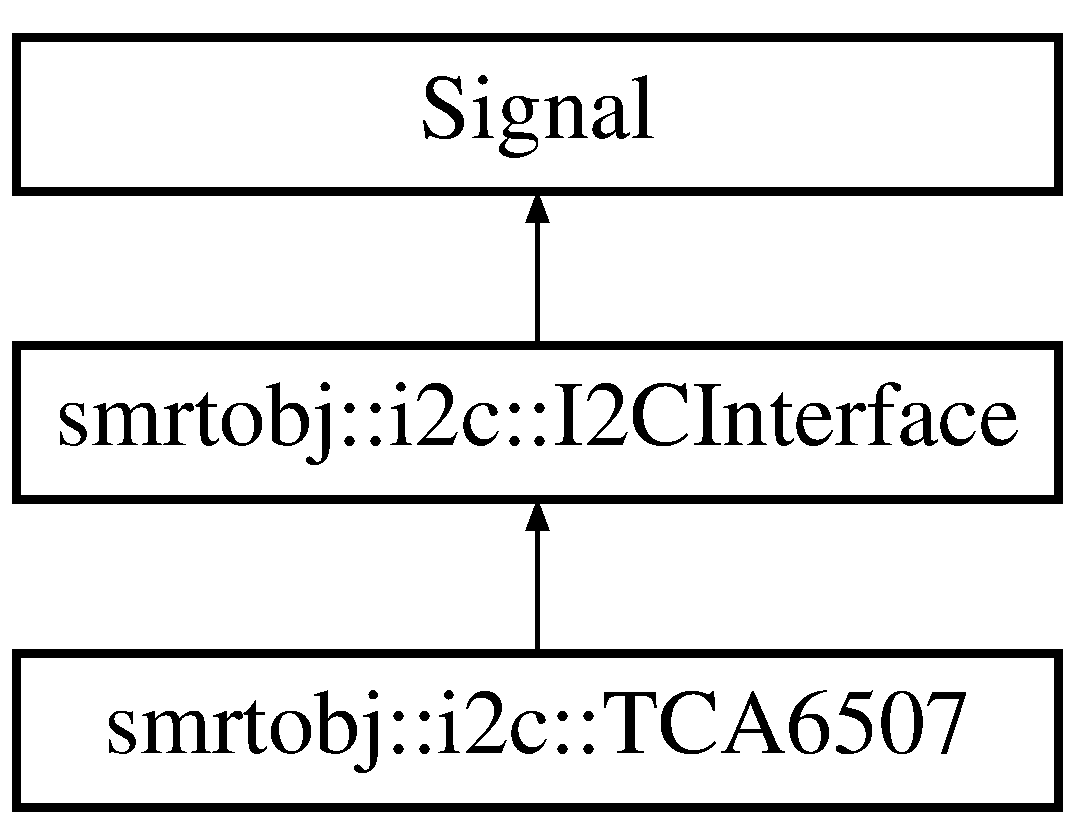
\includegraphics[height=3.000000cm]{classsmrtobj_1_1i2c_1_1_t_c_a6507}
\end{center}
\end{figure}
\subsection*{Public Types}
\begin{DoxyCompactItemize}
\item 
enum \hyperlink{classsmrtobj_1_1i2c_1_1_t_c_a6507_a2b771c2f4975065352874dc67f7d701d}{\+\_\+cmd\+\_\+control\+\_\+register} \{ \\*
\hyperlink{classsmrtobj_1_1i2c_1_1_t_c_a6507_a2b771c2f4975065352874dc67f7d701dac115aeb0ec43a2d83c19d4e7ebfcc019}{S\+E\+L\+E\+C\+T0} = 0x00, 
\hyperlink{classsmrtobj_1_1i2c_1_1_t_c_a6507_a2b771c2f4975065352874dc67f7d701da80e0d021063c8c95043a18096a6f55f6}{S\+E\+L\+E\+C\+T1} = 0x01, 
\hyperlink{classsmrtobj_1_1i2c_1_1_t_c_a6507_a2b771c2f4975065352874dc67f7d701da5d235daea8e318dd0019d311b61356e5}{S\+E\+L\+E\+C\+T2} = 0x02, 
\hyperlink{classsmrtobj_1_1i2c_1_1_t_c_a6507_a2b771c2f4975065352874dc67f7d701dadbe07d59e0b42489fe4630e742474706}{F\+A\+D\+E\+\_\+\+O\+N\+\_\+\+T\+I\+M\+E} = 0x03, 
\\*
\hyperlink{classsmrtobj_1_1i2c_1_1_t_c_a6507_a2b771c2f4975065352874dc67f7d701da3ee378f498643771b6ca05f694f958df}{F\+U\+L\+L\+Y\+\_\+\+O\+N\+\_\+\+T\+I\+M\+E} = 0x04, 
\hyperlink{classsmrtobj_1_1i2c_1_1_t_c_a6507_a2b771c2f4975065352874dc67f7d701da41b2e6199f4780872cb7258e68778a38}{F\+A\+D\+E\+\_\+\+O\+F\+F\+\_\+\+T\+I\+M\+E} = 0x05, 
\hyperlink{classsmrtobj_1_1i2c_1_1_t_c_a6507_a2b771c2f4975065352874dc67f7d701da19da634d7d0500d0183c84b38a27913b}{F\+I\+R\+S\+T\+\_\+\+F\+U\+L\+L\+Y\+\_\+\+O\+F\+F\+\_\+\+T\+I\+M\+E} = 0x06, 
\hyperlink{classsmrtobj_1_1i2c_1_1_t_c_a6507_a2b771c2f4975065352874dc67f7d701dad71604546cc54ed7555ef07cde91eabb}{S\+E\+C\+O\+N\+D\+\_\+\+F\+U\+L\+L\+Y\+\_\+\+O\+F\+F\+\_\+\+T\+I\+M\+E} = 0x07, 
\\*
\hyperlink{classsmrtobj_1_1i2c_1_1_t_c_a6507_a2b771c2f4975065352874dc67f7d701daaf48f3426047c446eaba5ec6794882a2}{M\+A\+X\+I\+M\+U\+M\+\_\+\+I\+N\+T\+E\+N\+S\+I\+T\+Y} = 0x08, 
\hyperlink{classsmrtobj_1_1i2c_1_1_t_c_a6507_a2b771c2f4975065352874dc67f7d701daade32326b81b35ec16d594c1ec889e59}{O\+N\+E\+\_\+\+S\+H\+O\+T} = 0x09, 
\hyperlink{classsmrtobj_1_1i2c_1_1_t_c_a6507_a2b771c2f4975065352874dc67f7d701daf19ec560d33bb6cc1765341b8a4016d9}{I\+N\+I\+T\+I\+A\+L\+I\+Z\+A\+T\+I\+O\+N} = 0x10
 \}
\item 
enum \hyperlink{classsmrtobj_1_1i2c_1_1_t_c_a6507_a22d31cb7c3a277375d30c8ae5de03989}{\+\_\+register\+\_\+description} \{ \\*
\hyperlink{classsmrtobj_1_1i2c_1_1_t_c_a6507_a22d31cb7c3a277375d30c8ae5de03989a6368505486a80eb65a7857e0abc579ad}{L\+E\+D\+\_\+\+O\+F\+F} = 0x00, 
\hyperlink{classsmrtobj_1_1i2c_1_1_t_c_a6507_a22d31cb7c3a277375d30c8ae5de03989ab3f7bc8f1df8b218a0897eeaa584f274}{L\+E\+D\+\_\+\+O\+N\+\_\+\+P\+W\+M0} = 0x02, 
\hyperlink{classsmrtobj_1_1i2c_1_1_t_c_a6507_a22d31cb7c3a277375d30c8ae5de03989a993c4a080f8ec7d1b5d79a2543e8a5db}{L\+E\+D\+\_\+\+O\+N\+\_\+\+P\+W\+M1} = 0x03, 
\hyperlink{classsmrtobj_1_1i2c_1_1_t_c_a6507_a22d31cb7c3a277375d30c8ae5de03989a421b694853eaa4fe48b0ea668c9bc043}{L\+E\+D\+\_\+\+O\+N} = 0x04, 
\\*
\hyperlink{classsmrtobj_1_1i2c_1_1_t_c_a6507_a22d31cb7c3a277375d30c8ae5de03989a0724eabc40880f0d699e545628309936}{L\+E\+D\+\_\+\+O\+N\+\_\+\+O\+N\+E\+\_\+\+S\+H\+O\+T} = 0x05, 
\hyperlink{classsmrtobj_1_1i2c_1_1_t_c_a6507_a22d31cb7c3a277375d30c8ae5de03989abdabd46acaec7532efff2e35a3705f38}{L\+E\+D\+\_\+\+B\+L\+I\+N\+K\+\_\+\+B\+A\+N\+K0} = 0x06, 
\hyperlink{classsmrtobj_1_1i2c_1_1_t_c_a6507_a22d31cb7c3a277375d30c8ae5de03989aa72f6202fc594ba0bfd7b502cb1237c6}{L\+E\+D\+\_\+\+B\+L\+I\+N\+K\+\_\+\+B\+A\+N\+K1} = 0x07
 \}
\item 
enum \hyperlink{classsmrtobj_1_1i2c_1_1_t_c_a6507_a06dd5b58f4a44a9e76e1a7620f353e54}{\+\_\+output\+\_\+pin} \{ \\*
\hyperlink{classsmrtobj_1_1i2c_1_1_t_c_a6507_a06dd5b58f4a44a9e76e1a7620f353e54aee5120419f091947eec5d2478acdf1f9}{P0} = 0x00, 
\hyperlink{classsmrtobj_1_1i2c_1_1_t_c_a6507_a06dd5b58f4a44a9e76e1a7620f353e54ad12892b31428bc0ecc255e52fef6ac8e}{P1} = 0x01, 
\hyperlink{classsmrtobj_1_1i2c_1_1_t_c_a6507_a06dd5b58f4a44a9e76e1a7620f353e54a5b5374c6ba12ab94407cd773e10fff5d}{P2} = 0x02, 
\hyperlink{classsmrtobj_1_1i2c_1_1_t_c_a6507_a06dd5b58f4a44a9e76e1a7620f353e54a723ef58bc7f102842fef3ecc2bb44476}{P3} = 0x03, 
\\*
\hyperlink{classsmrtobj_1_1i2c_1_1_t_c_a6507_a06dd5b58f4a44a9e76e1a7620f353e54a0615bfc9748b3e015912a05c52a90320}{P4} = 0x04, 
\hyperlink{classsmrtobj_1_1i2c_1_1_t_c_a6507_a06dd5b58f4a44a9e76e1a7620f353e54af7c9898266358e93e6bf3b18d954d32d}{P5} = 0x05, 
\hyperlink{classsmrtobj_1_1i2c_1_1_t_c_a6507_a06dd5b58f4a44a9e76e1a7620f353e54a53dccb9143383f84dc178097151664c5}{P6} = 0x06
 \}
\item 
enum \hyperlink{classsmrtobj_1_1i2c_1_1_t_c_a6507_abdc67db030169d80977a45f6a6917956}{\+\_\+time\+\_\+parameter} \{ \\*
\hyperlink{classsmrtobj_1_1i2c_1_1_t_c_a6507_abdc67db030169d80977a45f6a6917956a00e9621ed594f4229ff0eadfb9d3ab31}{T\+M\+S0} = 0x00, 
\hyperlink{classsmrtobj_1_1i2c_1_1_t_c_a6507_abdc67db030169d80977a45f6a6917956a0fff1807c60d3cf32af947465a308eac}{T\+M\+S64} = 0x01, 
\hyperlink{classsmrtobj_1_1i2c_1_1_t_c_a6507_abdc67db030169d80977a45f6a6917956a74d9a7c8b89bd2945ba0b4d30281573b}{T\+M\+S128} = 0x02, 
\hyperlink{classsmrtobj_1_1i2c_1_1_t_c_a6507_abdc67db030169d80977a45f6a6917956a937978928c3c72a1bdafc1c1e4be5e84}{T\+M\+S192} = 0x03, 
\\*
\hyperlink{classsmrtobj_1_1i2c_1_1_t_c_a6507_abdc67db030169d80977a45f6a6917956a8498e4d04fa036047e38c6318b84b0dc}{T\+M\+S256} = 0x04, 
\hyperlink{classsmrtobj_1_1i2c_1_1_t_c_a6507_abdc67db030169d80977a45f6a6917956ac9520e6ba3081898800b89c28772d2a3}{T\+M\+S384} = 0x05, 
\hyperlink{classsmrtobj_1_1i2c_1_1_t_c_a6507_abdc67db030169d80977a45f6a6917956acdf4742bc7f2da3f7c22c4a007b3bc1c}{T\+M\+S512} = 0x06, 
\hyperlink{classsmrtobj_1_1i2c_1_1_t_c_a6507_abdc67db030169d80977a45f6a6917956a45e18e8b4cfa4dd2db77f7542b4ec70d}{T\+M\+S768} = 0x07, 
\\*
\hyperlink{classsmrtobj_1_1i2c_1_1_t_c_a6507_abdc67db030169d80977a45f6a6917956a0a673fb2319621650d7814f4173f5cc2}{T\+M\+S1024} = 0x08, 
\hyperlink{classsmrtobj_1_1i2c_1_1_t_c_a6507_abdc67db030169d80977a45f6a6917956a145bb090c4464beeb2b7ddce679e28dc}{T\+M\+S1536} = 0x09, 
\hyperlink{classsmrtobj_1_1i2c_1_1_t_c_a6507_abdc67db030169d80977a45f6a6917956ae48f87f89ac1af384c8ea44e5d1f4802}{T\+M\+S2048} = 0x0\+A, 
\hyperlink{classsmrtobj_1_1i2c_1_1_t_c_a6507_abdc67db030169d80977a45f6a6917956aa9034903f1d9721c22703ab14e2f8dbc}{T\+M\+S3072} = 0x0\+B, 
\\*
\hyperlink{classsmrtobj_1_1i2c_1_1_t_c_a6507_abdc67db030169d80977a45f6a6917956a0c1b13c9fe6f990f7df881c87c0248d1}{T\+M\+S4096} = 0x0\+C, 
\hyperlink{classsmrtobj_1_1i2c_1_1_t_c_a6507_abdc67db030169d80977a45f6a6917956a1aa07bd02b2536915b26af2401c6bf45}{T\+M\+S5760} = 0x0\+D, 
\hyperlink{classsmrtobj_1_1i2c_1_1_t_c_a6507_abdc67db030169d80977a45f6a6917956a0f44120a579fcc618dbb05450eec8dda}{T\+M\+S8128} = 0x0\+E, 
\hyperlink{classsmrtobj_1_1i2c_1_1_t_c_a6507_abdc67db030169d80977a45f6a6917956a2e1a20e1bca96a743e3709d8ba6dd02f}{T\+M\+S16320} = 0x0\+F
 \}
\item 
enum \hyperlink{classsmrtobj_1_1i2c_1_1_t_c_a6507_a416c966fabb333b9b60a2e62f674e3ec}{\+\_\+basic\+\_\+bank\+\_\+number} \{ \hyperlink{classsmrtobj_1_1i2c_1_1_t_c_a6507_a416c966fabb333b9b60a2e62f674e3eca375a3de4e50bd869dfc248e139974527}{B\+A\+N\+K0} = 0x00, 
\hyperlink{classsmrtobj_1_1i2c_1_1_t_c_a6507_a416c966fabb333b9b60a2e62f674e3eca45b9000ef40886cbb3a6ce9053d4e246}{B\+A\+N\+K1} = 0x01
 \}
\end{DoxyCompactItemize}
\subsection*{Public Member Functions}
\begin{DoxyCompactItemize}
\item 
\hyperlink{classsmrtobj_1_1i2c_1_1_t_c_a6507_a150f61534c180db5eae06eabe84a23ff}{T\+C\+A6507} ()
\item 
\hyperlink{classsmrtobj_1_1i2c_1_1_t_c_a6507_a34e833d577e689c85df1a38cbe8597e0}{T\+C\+A6507} (uint8\+\_\+t r\+\_\+pin)
\item 
\hyperlink{classsmrtobj_1_1i2c_1_1_t_c_a6507_acdae96b9ad4df69b7db373b741875af9}{T\+C\+A6507} (const \hyperlink{classsmrtobj_1_1i2c_1_1_t_c_a6507}{T\+C\+A6507} \&d)
\item 
virtual \hyperlink{classsmrtobj_1_1i2c_1_1_t_c_a6507_ac71dca60bfff937556402fb8d4e74c94}{$\sim$\+T\+C\+A6507} ()
\item 
\hyperlink{classsmrtobj_1_1i2c_1_1_t_c_a6507}{T\+C\+A6507} \& \hyperlink{classsmrtobj_1_1i2c_1_1_t_c_a6507_a97c3c53eb57784c8443c05a6d8c8e67b}{operator=} (const \hyperlink{classsmrtobj_1_1i2c_1_1_t_c_a6507}{T\+C\+A6507} \&d)
\item 
virtual bool \hyperlink{classsmrtobj_1_1i2c_1_1_t_c_a6507_a630cc83b260aceec29c3f26e2c4ebe5e}{initialize} ()
\item 
void \hyperlink{classsmrtobj_1_1i2c_1_1_t_c_a6507_a34361f72e69f4342dbdd9e324fd3e13a}{start} ()
\item 
void \hyperlink{classsmrtobj_1_1i2c_1_1_t_c_a6507_a6f16cbe2d218b6c1a9182d67e2da20ac}{stop} ()
\item 
virtual bool \hyperlink{classsmrtobj_1_1i2c_1_1_t_c_a6507_adce687bb4bd2f248a1851b5d3e290181}{read} ()
\item 
virtual bool \hyperlink{classsmrtobj_1_1i2c_1_1_t_c_a6507_aae2ceb7c2ba719a2d86d47f58cf16306}{is\+Connected} ()
\item 
bool \hyperlink{classsmrtobj_1_1i2c_1_1_t_c_a6507_a53e7478510f82ce0b0ac85ab58de6ba2}{R\+A\+W\+Sel\+Regs\+Drv} (uint8\+\_\+t s0, uint8\+\_\+t s1, uint8\+\_\+t s2)
\item 
bool \hyperlink{classsmrtobj_1_1i2c_1_1_t_c_a6507_a37124e71b06ed662f215d97305d3cc8b}{R\+A\+W\+Reg\+Drv} (uint8\+\_\+t reg, uint8\+\_\+t val)
\item 
uint8\+\_\+t \hyperlink{classsmrtobj_1_1i2c_1_1_t_c_a6507_a7453556043cf9fc41fa28f6076022d83}{read\+Reg} (uint8\+\_\+t reg)
\item 
uint8\+\_\+t \hyperlink{classsmrtobj_1_1i2c_1_1_t_c_a6507_a267ba5d392d1e12ad29842a3ff113a61}{pin\+State} (uint8\+\_\+t pin)
\item 
void \hyperlink{classsmrtobj_1_1i2c_1_1_t_c_a6507_af4c4bd40c4b32067f8e189e27cf05ef7}{pin\+Set\+State} (uint8\+\_\+t pin, uint8\+\_\+t state)
\item 
void \hyperlink{classsmrtobj_1_1i2c_1_1_t_c_a6507_aa5bc0319b630246d0e8bd337b6c311ca}{basic\+Bank\+Setup} (uint8\+\_\+t n\+Bank, uint8\+\_\+t fade\+On, uint8\+\_\+t on\+Time, uint8\+\_\+t fade\+Off, uint8\+\_\+t off\+Time, uint8\+\_\+t sd\+Off\+Time)
\item 
void \hyperlink{classsmrtobj_1_1i2c_1_1_t_c_a6507_afba268a027f4792556f8fe57a424a1f1}{registry\+To\+Bank} (uint8\+\_\+t n\+Bank, uint8\+\_\+t n\+Reg, uint8\+\_\+t val)
\end{DoxyCompactItemize}
\subsection*{Static Public Attributes}
\begin{DoxyCompactItemize}
\item 
\hypertarget{classsmrtobj_1_1i2c_1_1_t_c_a6507_ad8c7f82e183bef0f41de9c5a373f9a97}{}static const uint8\+\_\+t \hyperlink{classsmrtobj_1_1i2c_1_1_t_c_a6507_ad8c7f82e183bef0f41de9c5a373f9a97}{D\+E\+V\+I\+C\+E\+\_\+\+A\+D\+D\+R\+E\+S\+S} = 0x45\label{classsmrtobj_1_1i2c_1_1_t_c_a6507_ad8c7f82e183bef0f41de9c5a373f9a97}

\begin{DoxyCompactList}\small\item\em Device address used by default. \end{DoxyCompactList}\end{DoxyCompactItemize}
\subsection*{Additional Inherited Members}


\subsection{Detailed Description}
Class \hyperlink{classsmrtobj_1_1i2c_1_1_t_c_a6507}{T\+C\+A6507} models the \hyperlink{classsmrtobj_1_1i2c_1_1_t_c_a6507}{T\+C\+A6507} L\+E\+D driver using I2\+C protocol. This 7-\/bit L\+E\+D dimmer for the two-\/line bidirectional bus (I2\+C) is designed to control (or dim) L\+E\+Ds via the I2\+C interface. Without this device, the microprocessor or microcontroller must be actively involved in turning on and off the L\+E\+Ds (per the required dimming rate), which uses valuable processor time and the overloads I2\+C bus. The \hyperlink{classsmrtobj_1_1i2c_1_1_t_c_a6507}{T\+C\+A6507} alleviates this issue by limiting the number of operations required by the processor in blinking L\+E\+Ds and, thus, helps to create a more efficient system. 

Definition at line 29 of file T\+C\+A6507.\+h.



\subsection{Member Enumeration Documentation}
\hypertarget{classsmrtobj_1_1i2c_1_1_t_c_a6507_a416c966fabb333b9b60a2e62f674e3ec}{}\index{smrtobj\+::i2c\+::\+T\+C\+A6507@{smrtobj\+::i2c\+::\+T\+C\+A6507}!\+\_\+basic\+\_\+bank\+\_\+number@{\+\_\+basic\+\_\+bank\+\_\+number}}
\index{\+\_\+basic\+\_\+bank\+\_\+number@{\+\_\+basic\+\_\+bank\+\_\+number}!smrtobj\+::i2c\+::\+T\+C\+A6507@{smrtobj\+::i2c\+::\+T\+C\+A6507}}
\subsubsection[{\+\_\+basic\+\_\+bank\+\_\+number}]{\setlength{\rightskip}{0pt plus 5cm}enum {\bf smrtobj\+::i2c\+::\+T\+C\+A6507\+::\+\_\+basic\+\_\+bank\+\_\+number}}\label{classsmrtobj_1_1i2c_1_1_t_c_a6507_a416c966fabb333b9b60a2e62f674e3ec}
Basic bank number. \begin{Desc}
\item[Enumerator]\par
\begin{description}
\index{B\+A\+N\+K0@{B\+A\+N\+K0}!smrtobj\+::i2c\+::\+T\+C\+A6507@{smrtobj\+::i2c\+::\+T\+C\+A6507}}\index{smrtobj\+::i2c\+::\+T\+C\+A6507@{smrtobj\+::i2c\+::\+T\+C\+A6507}!B\+A\+N\+K0@{B\+A\+N\+K0}}\item[{\em 
\hypertarget{classsmrtobj_1_1i2c_1_1_t_c_a6507_a416c966fabb333b9b60a2e62f674e3eca375a3de4e50bd869dfc248e139974527}{}B\+A\+N\+K0\label{classsmrtobj_1_1i2c_1_1_t_c_a6507_a416c966fabb333b9b60a2e62f674e3eca375a3de4e50bd869dfc248e139974527}
}]Bank 0. \index{B\+A\+N\+K1@{B\+A\+N\+K1}!smrtobj\+::i2c\+::\+T\+C\+A6507@{smrtobj\+::i2c\+::\+T\+C\+A6507}}\index{smrtobj\+::i2c\+::\+T\+C\+A6507@{smrtobj\+::i2c\+::\+T\+C\+A6507}!B\+A\+N\+K1@{B\+A\+N\+K1}}\item[{\em 
\hypertarget{classsmrtobj_1_1i2c_1_1_t_c_a6507_a416c966fabb333b9b60a2e62f674e3eca45b9000ef40886cbb3a6ce9053d4e246}{}B\+A\+N\+K1\label{classsmrtobj_1_1i2c_1_1_t_c_a6507_a416c966fabb333b9b60a2e62f674e3eca45b9000ef40886cbb3a6ce9053d4e246}
}]Bank 1. \end{description}
\end{Desc}


Definition at line 196 of file T\+C\+A6507.\+h.

\hypertarget{classsmrtobj_1_1i2c_1_1_t_c_a6507_a2b771c2f4975065352874dc67f7d701d}{}\index{smrtobj\+::i2c\+::\+T\+C\+A6507@{smrtobj\+::i2c\+::\+T\+C\+A6507}!\+\_\+cmd\+\_\+control\+\_\+register@{\+\_\+cmd\+\_\+control\+\_\+register}}
\index{\+\_\+cmd\+\_\+control\+\_\+register@{\+\_\+cmd\+\_\+control\+\_\+register}!smrtobj\+::i2c\+::\+T\+C\+A6507@{smrtobj\+::i2c\+::\+T\+C\+A6507}}
\subsubsection[{\+\_\+cmd\+\_\+control\+\_\+register}]{\setlength{\rightskip}{0pt plus 5cm}enum {\bf smrtobj\+::i2c\+::\+T\+C\+A6507\+::\+\_\+cmd\+\_\+control\+\_\+register}}\label{classsmrtobj_1_1i2c_1_1_t_c_a6507_a2b771c2f4975065352874dc67f7d701d}
Command byte for Control Register. Following the successful acknowledgment of the address byte, the bus master sends a command byte, which is stored in the control register. The last four bits (B0, B1, B2 and B3) of this command byte determine the internal registers (Select0, Select1, Select2, Fade-\/\+On Time, Fully-\/\+On Time, Fade-\/\+Off Time, First Fully-\/\+Off Time, Second Fully-\/\+Off Time, Maximum Intensity and Initialization) that are affected. The command byte is sent only during a write transmission. After the command byte is received, the I2\+C master starts sending data bytes. For more information read data sheet \href{http://www.ti.com/lit/ds/symlink/tca6507.pdf}{\tt http\+://www.\+ti.\+com/lit/ds/symlink/tca6507.\+pdf} \begin{Desc}
\item[Enumerator]\par
\begin{description}
\index{S\+E\+L\+E\+C\+T0@{S\+E\+L\+E\+C\+T0}!smrtobj\+::i2c\+::\+T\+C\+A6507@{smrtobj\+::i2c\+::\+T\+C\+A6507}}\index{smrtobj\+::i2c\+::\+T\+C\+A6507@{smrtobj\+::i2c\+::\+T\+C\+A6507}!S\+E\+L\+E\+C\+T0@{S\+E\+L\+E\+C\+T0}}\item[{\em 
\hypertarget{classsmrtobj_1_1i2c_1_1_t_c_a6507_a2b771c2f4975065352874dc67f7d701dac115aeb0ec43a2d83c19d4e7ebfcc019}{}S\+E\+L\+E\+C\+T0\label{classsmrtobj_1_1i2c_1_1_t_c_a6507_a2b771c2f4975065352874dc67f7d701dac115aeb0ec43a2d83c19d4e7ebfcc019}
}]\textquotesingle{}Command Select0\textquotesingle{} \index{S\+E\+L\+E\+C\+T1@{S\+E\+L\+E\+C\+T1}!smrtobj\+::i2c\+::\+T\+C\+A6507@{smrtobj\+::i2c\+::\+T\+C\+A6507}}\index{smrtobj\+::i2c\+::\+T\+C\+A6507@{smrtobj\+::i2c\+::\+T\+C\+A6507}!S\+E\+L\+E\+C\+T1@{S\+E\+L\+E\+C\+T1}}\item[{\em 
\hypertarget{classsmrtobj_1_1i2c_1_1_t_c_a6507_a2b771c2f4975065352874dc67f7d701da80e0d021063c8c95043a18096a6f55f6}{}S\+E\+L\+E\+C\+T1\label{classsmrtobj_1_1i2c_1_1_t_c_a6507_a2b771c2f4975065352874dc67f7d701da80e0d021063c8c95043a18096a6f55f6}
}]Command \textquotesingle{}Select1\textquotesingle{}. \index{S\+E\+L\+E\+C\+T2@{S\+E\+L\+E\+C\+T2}!smrtobj\+::i2c\+::\+T\+C\+A6507@{smrtobj\+::i2c\+::\+T\+C\+A6507}}\index{smrtobj\+::i2c\+::\+T\+C\+A6507@{smrtobj\+::i2c\+::\+T\+C\+A6507}!S\+E\+L\+E\+C\+T2@{S\+E\+L\+E\+C\+T2}}\item[{\em 
\hypertarget{classsmrtobj_1_1i2c_1_1_t_c_a6507_a2b771c2f4975065352874dc67f7d701da5d235daea8e318dd0019d311b61356e5}{}S\+E\+L\+E\+C\+T2\label{classsmrtobj_1_1i2c_1_1_t_c_a6507_a2b771c2f4975065352874dc67f7d701da5d235daea8e318dd0019d311b61356e5}
}]Command \textquotesingle{}Select2\textquotesingle{}. \index{F\+A\+D\+E\+\_\+\+O\+N\+\_\+\+T\+I\+M\+E@{F\+A\+D\+E\+\_\+\+O\+N\+\_\+\+T\+I\+M\+E}!smrtobj\+::i2c\+::\+T\+C\+A6507@{smrtobj\+::i2c\+::\+T\+C\+A6507}}\index{smrtobj\+::i2c\+::\+T\+C\+A6507@{smrtobj\+::i2c\+::\+T\+C\+A6507}!F\+A\+D\+E\+\_\+\+O\+N\+\_\+\+T\+I\+M\+E@{F\+A\+D\+E\+\_\+\+O\+N\+\_\+\+T\+I\+M\+E}}\item[{\em 
\hypertarget{classsmrtobj_1_1i2c_1_1_t_c_a6507_a2b771c2f4975065352874dc67f7d701dadbe07d59e0b42489fe4630e742474706}{}F\+A\+D\+E\+\_\+\+O\+N\+\_\+\+T\+I\+M\+E\label{classsmrtobj_1_1i2c_1_1_t_c_a6507_a2b771c2f4975065352874dc67f7d701dadbe07d59e0b42489fe4630e742474706}
}]Command \textquotesingle{}Fade-\/\+On Time\textquotesingle{}. \index{F\+U\+L\+L\+Y\+\_\+\+O\+N\+\_\+\+T\+I\+M\+E@{F\+U\+L\+L\+Y\+\_\+\+O\+N\+\_\+\+T\+I\+M\+E}!smrtobj\+::i2c\+::\+T\+C\+A6507@{smrtobj\+::i2c\+::\+T\+C\+A6507}}\index{smrtobj\+::i2c\+::\+T\+C\+A6507@{smrtobj\+::i2c\+::\+T\+C\+A6507}!F\+U\+L\+L\+Y\+\_\+\+O\+N\+\_\+\+T\+I\+M\+E@{F\+U\+L\+L\+Y\+\_\+\+O\+N\+\_\+\+T\+I\+M\+E}}\item[{\em 
\hypertarget{classsmrtobj_1_1i2c_1_1_t_c_a6507_a2b771c2f4975065352874dc67f7d701da3ee378f498643771b6ca05f694f958df}{}F\+U\+L\+L\+Y\+\_\+\+O\+N\+\_\+\+T\+I\+M\+E\label{classsmrtobj_1_1i2c_1_1_t_c_a6507_a2b771c2f4975065352874dc67f7d701da3ee378f498643771b6ca05f694f958df}
}]Command \textquotesingle{}Fully-\/\+On Time\textquotesingle{}. \index{F\+A\+D\+E\+\_\+\+O\+F\+F\+\_\+\+T\+I\+M\+E@{F\+A\+D\+E\+\_\+\+O\+F\+F\+\_\+\+T\+I\+M\+E}!smrtobj\+::i2c\+::\+T\+C\+A6507@{smrtobj\+::i2c\+::\+T\+C\+A6507}}\index{smrtobj\+::i2c\+::\+T\+C\+A6507@{smrtobj\+::i2c\+::\+T\+C\+A6507}!F\+A\+D\+E\+\_\+\+O\+F\+F\+\_\+\+T\+I\+M\+E@{F\+A\+D\+E\+\_\+\+O\+F\+F\+\_\+\+T\+I\+M\+E}}\item[{\em 
\hypertarget{classsmrtobj_1_1i2c_1_1_t_c_a6507_a2b771c2f4975065352874dc67f7d701da41b2e6199f4780872cb7258e68778a38}{}F\+A\+D\+E\+\_\+\+O\+F\+F\+\_\+\+T\+I\+M\+E\label{classsmrtobj_1_1i2c_1_1_t_c_a6507_a2b771c2f4975065352874dc67f7d701da41b2e6199f4780872cb7258e68778a38}
}]Command \textquotesingle{}Fade-\/\+Off Time\textquotesingle{}. \index{F\+I\+R\+S\+T\+\_\+\+F\+U\+L\+L\+Y\+\_\+\+O\+F\+F\+\_\+\+T\+I\+M\+E@{F\+I\+R\+S\+T\+\_\+\+F\+U\+L\+L\+Y\+\_\+\+O\+F\+F\+\_\+\+T\+I\+M\+E}!smrtobj\+::i2c\+::\+T\+C\+A6507@{smrtobj\+::i2c\+::\+T\+C\+A6507}}\index{smrtobj\+::i2c\+::\+T\+C\+A6507@{smrtobj\+::i2c\+::\+T\+C\+A6507}!F\+I\+R\+S\+T\+\_\+\+F\+U\+L\+L\+Y\+\_\+\+O\+F\+F\+\_\+\+T\+I\+M\+E@{F\+I\+R\+S\+T\+\_\+\+F\+U\+L\+L\+Y\+\_\+\+O\+F\+F\+\_\+\+T\+I\+M\+E}}\item[{\em 
\hypertarget{classsmrtobj_1_1i2c_1_1_t_c_a6507_a2b771c2f4975065352874dc67f7d701da19da634d7d0500d0183c84b38a27913b}{}F\+I\+R\+S\+T\+\_\+\+F\+U\+L\+L\+Y\+\_\+\+O\+F\+F\+\_\+\+T\+I\+M\+E\label{classsmrtobj_1_1i2c_1_1_t_c_a6507_a2b771c2f4975065352874dc67f7d701da19da634d7d0500d0183c84b38a27913b}
}]Command \textquotesingle{}First Fully-\/\+Off Time\textquotesingle{}. \index{S\+E\+C\+O\+N\+D\+\_\+\+F\+U\+L\+L\+Y\+\_\+\+O\+F\+F\+\_\+\+T\+I\+M\+E@{S\+E\+C\+O\+N\+D\+\_\+\+F\+U\+L\+L\+Y\+\_\+\+O\+F\+F\+\_\+\+T\+I\+M\+E}!smrtobj\+::i2c\+::\+T\+C\+A6507@{smrtobj\+::i2c\+::\+T\+C\+A6507}}\index{smrtobj\+::i2c\+::\+T\+C\+A6507@{smrtobj\+::i2c\+::\+T\+C\+A6507}!S\+E\+C\+O\+N\+D\+\_\+\+F\+U\+L\+L\+Y\+\_\+\+O\+F\+F\+\_\+\+T\+I\+M\+E@{S\+E\+C\+O\+N\+D\+\_\+\+F\+U\+L\+L\+Y\+\_\+\+O\+F\+F\+\_\+\+T\+I\+M\+E}}\item[{\em 
\hypertarget{classsmrtobj_1_1i2c_1_1_t_c_a6507_a2b771c2f4975065352874dc67f7d701dad71604546cc54ed7555ef07cde91eabb}{}S\+E\+C\+O\+N\+D\+\_\+\+F\+U\+L\+L\+Y\+\_\+\+O\+F\+F\+\_\+\+T\+I\+M\+E\label{classsmrtobj_1_1i2c_1_1_t_c_a6507_a2b771c2f4975065352874dc67f7d701dad71604546cc54ed7555ef07cde91eabb}
}]Command \textquotesingle{}First Fully-\/\+Off Time\textquotesingle{}. \index{M\+A\+X\+I\+M\+U\+M\+\_\+\+I\+N\+T\+E\+N\+S\+I\+T\+Y@{M\+A\+X\+I\+M\+U\+M\+\_\+\+I\+N\+T\+E\+N\+S\+I\+T\+Y}!smrtobj\+::i2c\+::\+T\+C\+A6507@{smrtobj\+::i2c\+::\+T\+C\+A6507}}\index{smrtobj\+::i2c\+::\+T\+C\+A6507@{smrtobj\+::i2c\+::\+T\+C\+A6507}!M\+A\+X\+I\+M\+U\+M\+\_\+\+I\+N\+T\+E\+N\+S\+I\+T\+Y@{M\+A\+X\+I\+M\+U\+M\+\_\+\+I\+N\+T\+E\+N\+S\+I\+T\+Y}}\item[{\em 
\hypertarget{classsmrtobj_1_1i2c_1_1_t_c_a6507_a2b771c2f4975065352874dc67f7d701daaf48f3426047c446eaba5ec6794882a2}{}M\+A\+X\+I\+M\+U\+M\+\_\+\+I\+N\+T\+E\+N\+S\+I\+T\+Y\label{classsmrtobj_1_1i2c_1_1_t_c_a6507_a2b771c2f4975065352874dc67f7d701daaf48f3426047c446eaba5ec6794882a2}
}]Command \textquotesingle{}Maximum Intensity\textquotesingle{}. \index{O\+N\+E\+\_\+\+S\+H\+O\+T@{O\+N\+E\+\_\+\+S\+H\+O\+T}!smrtobj\+::i2c\+::\+T\+C\+A6507@{smrtobj\+::i2c\+::\+T\+C\+A6507}}\index{smrtobj\+::i2c\+::\+T\+C\+A6507@{smrtobj\+::i2c\+::\+T\+C\+A6507}!O\+N\+E\+\_\+\+S\+H\+O\+T@{O\+N\+E\+\_\+\+S\+H\+O\+T}}\item[{\em 
\hypertarget{classsmrtobj_1_1i2c_1_1_t_c_a6507_a2b771c2f4975065352874dc67f7d701daade32326b81b35ec16d594c1ec889e59}{}O\+N\+E\+\_\+\+S\+H\+O\+T\label{classsmrtobj_1_1i2c_1_1_t_c_a6507_a2b771c2f4975065352874dc67f7d701daade32326b81b35ec16d594c1ec889e59}
}]Command \textquotesingle{}One Shot / Master Intensity\textquotesingle{}. \index{I\+N\+I\+T\+I\+A\+L\+I\+Z\+A\+T\+I\+O\+N@{I\+N\+I\+T\+I\+A\+L\+I\+Z\+A\+T\+I\+O\+N}!smrtobj\+::i2c\+::\+T\+C\+A6507@{smrtobj\+::i2c\+::\+T\+C\+A6507}}\index{smrtobj\+::i2c\+::\+T\+C\+A6507@{smrtobj\+::i2c\+::\+T\+C\+A6507}!I\+N\+I\+T\+I\+A\+L\+I\+Z\+A\+T\+I\+O\+N@{I\+N\+I\+T\+I\+A\+L\+I\+Z\+A\+T\+I\+O\+N}}\item[{\em 
\hypertarget{classsmrtobj_1_1i2c_1_1_t_c_a6507_a2b771c2f4975065352874dc67f7d701daf19ec560d33bb6cc1765341b8a4016d9}{}I\+N\+I\+T\+I\+A\+L\+I\+Z\+A\+T\+I\+O\+N\label{classsmrtobj_1_1i2c_1_1_t_c_a6507_a2b771c2f4975065352874dc67f7d701daf19ec560d33bb6cc1765341b8a4016d9}
}]Command \textquotesingle{}initialization\textquotesingle{}. \end{description}
\end{Desc}


Definition at line 45 of file T\+C\+A6507.\+h.

\hypertarget{classsmrtobj_1_1i2c_1_1_t_c_a6507_a06dd5b58f4a44a9e76e1a7620f353e54}{}\index{smrtobj\+::i2c\+::\+T\+C\+A6507@{smrtobj\+::i2c\+::\+T\+C\+A6507}!\+\_\+output\+\_\+pin@{\+\_\+output\+\_\+pin}}
\index{\+\_\+output\+\_\+pin@{\+\_\+output\+\_\+pin}!smrtobj\+::i2c\+::\+T\+C\+A6507@{smrtobj\+::i2c\+::\+T\+C\+A6507}}
\subsubsection[{\+\_\+output\+\_\+pin}]{\setlength{\rightskip}{0pt plus 5cm}enum {\bf smrtobj\+::i2c\+::\+T\+C\+A6507\+::\+\_\+output\+\_\+pin}}\label{classsmrtobj_1_1i2c_1_1_t_c_a6507_a06dd5b58f4a44a9e76e1a7620f353e54}
Output pin. \begin{Desc}
\item[Enumerator]\par
\begin{description}
\index{P0@{P0}!smrtobj\+::i2c\+::\+T\+C\+A6507@{smrtobj\+::i2c\+::\+T\+C\+A6507}}\index{smrtobj\+::i2c\+::\+T\+C\+A6507@{smrtobj\+::i2c\+::\+T\+C\+A6507}!P0@{P0}}\item[{\em 
\hypertarget{classsmrtobj_1_1i2c_1_1_t_c_a6507_a06dd5b58f4a44a9e76e1a7620f353e54aee5120419f091947eec5d2478acdf1f9}{}P0\label{classsmrtobj_1_1i2c_1_1_t_c_a6507_a06dd5b58f4a44a9e76e1a7620f353e54aee5120419f091947eec5d2478acdf1f9}
}]Output pin number 0. \index{P1@{P1}!smrtobj\+::i2c\+::\+T\+C\+A6507@{smrtobj\+::i2c\+::\+T\+C\+A6507}}\index{smrtobj\+::i2c\+::\+T\+C\+A6507@{smrtobj\+::i2c\+::\+T\+C\+A6507}!P1@{P1}}\item[{\em 
\hypertarget{classsmrtobj_1_1i2c_1_1_t_c_a6507_a06dd5b58f4a44a9e76e1a7620f353e54ad12892b31428bc0ecc255e52fef6ac8e}{}P1\label{classsmrtobj_1_1i2c_1_1_t_c_a6507_a06dd5b58f4a44a9e76e1a7620f353e54ad12892b31428bc0ecc255e52fef6ac8e}
}]Output pin number 1. \index{P2@{P2}!smrtobj\+::i2c\+::\+T\+C\+A6507@{smrtobj\+::i2c\+::\+T\+C\+A6507}}\index{smrtobj\+::i2c\+::\+T\+C\+A6507@{smrtobj\+::i2c\+::\+T\+C\+A6507}!P2@{P2}}\item[{\em 
\hypertarget{classsmrtobj_1_1i2c_1_1_t_c_a6507_a06dd5b58f4a44a9e76e1a7620f353e54a5b5374c6ba12ab94407cd773e10fff5d}{}P2\label{classsmrtobj_1_1i2c_1_1_t_c_a6507_a06dd5b58f4a44a9e76e1a7620f353e54a5b5374c6ba12ab94407cd773e10fff5d}
}]Output pin number 2. \index{P3@{P3}!smrtobj\+::i2c\+::\+T\+C\+A6507@{smrtobj\+::i2c\+::\+T\+C\+A6507}}\index{smrtobj\+::i2c\+::\+T\+C\+A6507@{smrtobj\+::i2c\+::\+T\+C\+A6507}!P3@{P3}}\item[{\em 
\hypertarget{classsmrtobj_1_1i2c_1_1_t_c_a6507_a06dd5b58f4a44a9e76e1a7620f353e54a723ef58bc7f102842fef3ecc2bb44476}{}P3\label{classsmrtobj_1_1i2c_1_1_t_c_a6507_a06dd5b58f4a44a9e76e1a7620f353e54a723ef58bc7f102842fef3ecc2bb44476}
}]Output pin number 3. \index{P4@{P4}!smrtobj\+::i2c\+::\+T\+C\+A6507@{smrtobj\+::i2c\+::\+T\+C\+A6507}}\index{smrtobj\+::i2c\+::\+T\+C\+A6507@{smrtobj\+::i2c\+::\+T\+C\+A6507}!P4@{P4}}\item[{\em 
\hypertarget{classsmrtobj_1_1i2c_1_1_t_c_a6507_a06dd5b58f4a44a9e76e1a7620f353e54a0615bfc9748b3e015912a05c52a90320}{}P4\label{classsmrtobj_1_1i2c_1_1_t_c_a6507_a06dd5b58f4a44a9e76e1a7620f353e54a0615bfc9748b3e015912a05c52a90320}
}]Output pin number 4. \index{P5@{P5}!smrtobj\+::i2c\+::\+T\+C\+A6507@{smrtobj\+::i2c\+::\+T\+C\+A6507}}\index{smrtobj\+::i2c\+::\+T\+C\+A6507@{smrtobj\+::i2c\+::\+T\+C\+A6507}!P5@{P5}}\item[{\em 
\hypertarget{classsmrtobj_1_1i2c_1_1_t_c_a6507_a06dd5b58f4a44a9e76e1a7620f353e54af7c9898266358e93e6bf3b18d954d32d}{}P5\label{classsmrtobj_1_1i2c_1_1_t_c_a6507_a06dd5b58f4a44a9e76e1a7620f353e54af7c9898266358e93e6bf3b18d954d32d}
}]Output pin number 5. \index{P6@{P6}!smrtobj\+::i2c\+::\+T\+C\+A6507@{smrtobj\+::i2c\+::\+T\+C\+A6507}}\index{smrtobj\+::i2c\+::\+T\+C\+A6507@{smrtobj\+::i2c\+::\+T\+C\+A6507}!P6@{P6}}\item[{\em 
\hypertarget{classsmrtobj_1_1i2c_1_1_t_c_a6507_a06dd5b58f4a44a9e76e1a7620f353e54a53dccb9143383f84dc178097151664c5}{}P6\label{classsmrtobj_1_1i2c_1_1_t_c_a6507_a06dd5b58f4a44a9e76e1a7620f353e54a53dccb9143383f84dc178097151664c5}
}]Output pin number 6. \end{description}
\end{Desc}


Definition at line 114 of file T\+C\+A6507.\+h.

\hypertarget{classsmrtobj_1_1i2c_1_1_t_c_a6507_a22d31cb7c3a277375d30c8ae5de03989}{}\index{smrtobj\+::i2c\+::\+T\+C\+A6507@{smrtobj\+::i2c\+::\+T\+C\+A6507}!\+\_\+register\+\_\+description@{\+\_\+register\+\_\+description}}
\index{\+\_\+register\+\_\+description@{\+\_\+register\+\_\+description}!smrtobj\+::i2c\+::\+T\+C\+A6507@{smrtobj\+::i2c\+::\+T\+C\+A6507}}
\subsubsection[{\+\_\+register\+\_\+description}]{\setlength{\rightskip}{0pt plus 5cm}enum {\bf smrtobj\+::i2c\+::\+T\+C\+A6507\+::\+\_\+register\+\_\+description}}\label{classsmrtobj_1_1i2c_1_1_t_c_a6507_a22d31cb7c3a277375d30c8ae5de03989}
Register Descriptions. The Select0 register (register 0), Select1 (register 1), and Select2 register (register 2) configure the state of each of the outputs \begin{Desc}
\item[Enumerator]\par
\begin{description}
\index{L\+E\+D\+\_\+\+O\+F\+F@{L\+E\+D\+\_\+\+O\+F\+F}!smrtobj\+::i2c\+::\+T\+C\+A6507@{smrtobj\+::i2c\+::\+T\+C\+A6507}}\index{smrtobj\+::i2c\+::\+T\+C\+A6507@{smrtobj\+::i2c\+::\+T\+C\+A6507}!L\+E\+D\+\_\+\+O\+F\+F@{L\+E\+D\+\_\+\+O\+F\+F}}\item[{\em 
\hypertarget{classsmrtobj_1_1i2c_1_1_t_c_a6507_a22d31cb7c3a277375d30c8ae5de03989a6368505486a80eb65a7857e0abc579ad}{}L\+E\+D\+\_\+\+O\+F\+F\label{classsmrtobj_1_1i2c_1_1_t_c_a6507_a22d31cb7c3a277375d30c8ae5de03989a6368505486a80eb65a7857e0abc579ad}
}]L\+E\+D off (High impedence) \index{L\+E\+D\+\_\+\+O\+N\+\_\+\+P\+W\+M0@{L\+E\+D\+\_\+\+O\+N\+\_\+\+P\+W\+M0}!smrtobj\+::i2c\+::\+T\+C\+A6507@{smrtobj\+::i2c\+::\+T\+C\+A6507}}\index{smrtobj\+::i2c\+::\+T\+C\+A6507@{smrtobj\+::i2c\+::\+T\+C\+A6507}!L\+E\+D\+\_\+\+O\+N\+\_\+\+P\+W\+M0@{L\+E\+D\+\_\+\+O\+N\+\_\+\+P\+W\+M0}}\item[{\em 
\hypertarget{classsmrtobj_1_1i2c_1_1_t_c_a6507_a22d31cb7c3a277375d30c8ae5de03989ab3f7bc8f1df8b218a0897eeaa584f274}{}L\+E\+D\+\_\+\+O\+N\+\_\+\+P\+W\+M0\label{classsmrtobj_1_1i2c_1_1_t_c_a6507_a22d31cb7c3a277375d30c8ae5de03989ab3f7bc8f1df8b218a0897eeaa584f274}
}]L\+E\+D on steadily with maximum intensity value of P\+W\+M0 (A\+L\+D value or B\+R\+I\+G\+H\+T\+\_\+\+F0 value) \index{L\+E\+D\+\_\+\+O\+N\+\_\+\+P\+W\+M1@{L\+E\+D\+\_\+\+O\+N\+\_\+\+P\+W\+M1}!smrtobj\+::i2c\+::\+T\+C\+A6507@{smrtobj\+::i2c\+::\+T\+C\+A6507}}\index{smrtobj\+::i2c\+::\+T\+C\+A6507@{smrtobj\+::i2c\+::\+T\+C\+A6507}!L\+E\+D\+\_\+\+O\+N\+\_\+\+P\+W\+M1@{L\+E\+D\+\_\+\+O\+N\+\_\+\+P\+W\+M1}}\item[{\em 
\hypertarget{classsmrtobj_1_1i2c_1_1_t_c_a6507_a22d31cb7c3a277375d30c8ae5de03989a993c4a080f8ec7d1b5d79a2543e8a5db}{}L\+E\+D\+\_\+\+O\+N\+\_\+\+P\+W\+M1\label{classsmrtobj_1_1i2c_1_1_t_c_a6507_a22d31cb7c3a277375d30c8ae5de03989a993c4a080f8ec7d1b5d79a2543e8a5db}
}]L\+E\+D on steadily with maximum intensity value of P\+W\+M1 (A\+L\+D value or B\+R\+I\+G\+H\+T\+\_\+\+F1 value) \index{L\+E\+D\+\_\+\+O\+N@{L\+E\+D\+\_\+\+O\+N}!smrtobj\+::i2c\+::\+T\+C\+A6507@{smrtobj\+::i2c\+::\+T\+C\+A6507}}\index{smrtobj\+::i2c\+::\+T\+C\+A6507@{smrtobj\+::i2c\+::\+T\+C\+A6507}!L\+E\+D\+\_\+\+O\+N@{L\+E\+D\+\_\+\+O\+N}}\item[{\em 
\hypertarget{classsmrtobj_1_1i2c_1_1_t_c_a6507_a22d31cb7c3a277375d30c8ae5de03989a421b694853eaa4fe48b0ea668c9bc043}{}L\+E\+D\+\_\+\+O\+N\label{classsmrtobj_1_1i2c_1_1_t_c_a6507_a22d31cb7c3a277375d30c8ae5de03989a421b694853eaa4fe48b0ea668c9bc043}
}]L\+E\+D fully on (output low). Can be used as general-\/purpose output. \index{L\+E\+D\+\_\+\+O\+N\+\_\+\+O\+N\+E\+\_\+\+S\+H\+O\+T@{L\+E\+D\+\_\+\+O\+N\+\_\+\+O\+N\+E\+\_\+\+S\+H\+O\+T}!smrtobj\+::i2c\+::\+T\+C\+A6507@{smrtobj\+::i2c\+::\+T\+C\+A6507}}\index{smrtobj\+::i2c\+::\+T\+C\+A6507@{smrtobj\+::i2c\+::\+T\+C\+A6507}!L\+E\+D\+\_\+\+O\+N\+\_\+\+O\+N\+E\+\_\+\+S\+H\+O\+T@{L\+E\+D\+\_\+\+O\+N\+\_\+\+O\+N\+E\+\_\+\+S\+H\+O\+T}}\item[{\em 
\hypertarget{classsmrtobj_1_1i2c_1_1_t_c_a6507_a22d31cb7c3a277375d30c8ae5de03989a0724eabc40880f0d699e545628309936}{}L\+E\+D\+\_\+\+O\+N\+\_\+\+O\+N\+E\+\_\+\+S\+H\+O\+T\label{classsmrtobj_1_1i2c_1_1_t_c_a6507_a22d31cb7c3a277375d30c8ae5de03989a0724eabc40880f0d699e545628309936}
}]L\+E\+D on at brightness set by One Shot / Master Intensity register. \index{L\+E\+D\+\_\+\+B\+L\+I\+N\+K\+\_\+\+B\+A\+N\+K0@{L\+E\+D\+\_\+\+B\+L\+I\+N\+K\+\_\+\+B\+A\+N\+K0}!smrtobj\+::i2c\+::\+T\+C\+A6507@{smrtobj\+::i2c\+::\+T\+C\+A6507}}\index{smrtobj\+::i2c\+::\+T\+C\+A6507@{smrtobj\+::i2c\+::\+T\+C\+A6507}!L\+E\+D\+\_\+\+B\+L\+I\+N\+K\+\_\+\+B\+A\+N\+K0@{L\+E\+D\+\_\+\+B\+L\+I\+N\+K\+\_\+\+B\+A\+N\+K0}}\item[{\em 
\hypertarget{classsmrtobj_1_1i2c_1_1_t_c_a6507_a22d31cb7c3a277375d30c8ae5de03989abdabd46acaec7532efff2e35a3705f38}{}L\+E\+D\+\_\+\+B\+L\+I\+N\+K\+\_\+\+B\+A\+N\+K0\label{classsmrtobj_1_1i2c_1_1_t_c_a6507_a22d31cb7c3a277375d30c8ae5de03989abdabd46acaec7532efff2e35a3705f38}
}]L\+E\+D blinking with intensity characteristics of B\+A\+N\+K0 (P\+W\+M0) \index{L\+E\+D\+\_\+\+B\+L\+I\+N\+K\+\_\+\+B\+A\+N\+K1@{L\+E\+D\+\_\+\+B\+L\+I\+N\+K\+\_\+\+B\+A\+N\+K1}!smrtobj\+::i2c\+::\+T\+C\+A6507@{smrtobj\+::i2c\+::\+T\+C\+A6507}}\index{smrtobj\+::i2c\+::\+T\+C\+A6507@{smrtobj\+::i2c\+::\+T\+C\+A6507}!L\+E\+D\+\_\+\+B\+L\+I\+N\+K\+\_\+\+B\+A\+N\+K1@{L\+E\+D\+\_\+\+B\+L\+I\+N\+K\+\_\+\+B\+A\+N\+K1}}\item[{\em 
\hypertarget{classsmrtobj_1_1i2c_1_1_t_c_a6507_a22d31cb7c3a277375d30c8ae5de03989aa72f6202fc594ba0bfd7b502cb1237c6}{}L\+E\+D\+\_\+\+B\+L\+I\+N\+K\+\_\+\+B\+A\+N\+K1\label{classsmrtobj_1_1i2c_1_1_t_c_a6507_a22d31cb7c3a277375d30c8ae5de03989aa72f6202fc594ba0bfd7b502cb1237c6}
}]L\+E\+D blinking with intensity characteristics of B\+A\+N\+K1 (P\+W\+M1) \end{description}
\end{Desc}


Definition at line 87 of file T\+C\+A6507.\+h.

\hypertarget{classsmrtobj_1_1i2c_1_1_t_c_a6507_abdc67db030169d80977a45f6a6917956}{}\index{smrtobj\+::i2c\+::\+T\+C\+A6507@{smrtobj\+::i2c\+::\+T\+C\+A6507}!\+\_\+time\+\_\+parameter@{\+\_\+time\+\_\+parameter}}
\index{\+\_\+time\+\_\+parameter@{\+\_\+time\+\_\+parameter}!smrtobj\+::i2c\+::\+T\+C\+A6507@{smrtobj\+::i2c\+::\+T\+C\+A6507}}
\subsubsection[{\+\_\+time\+\_\+parameter}]{\setlength{\rightskip}{0pt plus 5cm}enum {\bf smrtobj\+::i2c\+::\+T\+C\+A6507\+::\+\_\+time\+\_\+parameter}}\label{classsmrtobj_1_1i2c_1_1_t_c_a6507_abdc67db030169d80977a45f6a6917956}
Value for the time parameter. \begin{Desc}
\item[Enumerator]\par
\begin{description}
\index{T\+M\+S0@{T\+M\+S0}!smrtobj\+::i2c\+::\+T\+C\+A6507@{smrtobj\+::i2c\+::\+T\+C\+A6507}}\index{smrtobj\+::i2c\+::\+T\+C\+A6507@{smrtobj\+::i2c\+::\+T\+C\+A6507}!T\+M\+S0@{T\+M\+S0}}\item[{\em 
\hypertarget{classsmrtobj_1_1i2c_1_1_t_c_a6507_abdc67db030169d80977a45f6a6917956a00e9621ed594f4229ff0eadfb9d3ab31}{}T\+M\+S0\label{classsmrtobj_1_1i2c_1_1_t_c_a6507_abdc67db030169d80977a45f6a6917956a00e9621ed594f4229ff0eadfb9d3ab31}
}]0 ms \index{T\+M\+S64@{T\+M\+S64}!smrtobj\+::i2c\+::\+T\+C\+A6507@{smrtobj\+::i2c\+::\+T\+C\+A6507}}\index{smrtobj\+::i2c\+::\+T\+C\+A6507@{smrtobj\+::i2c\+::\+T\+C\+A6507}!T\+M\+S64@{T\+M\+S64}}\item[{\em 
\hypertarget{classsmrtobj_1_1i2c_1_1_t_c_a6507_abdc67db030169d80977a45f6a6917956a0fff1807c60d3cf32af947465a308eac}{}T\+M\+S64\label{classsmrtobj_1_1i2c_1_1_t_c_a6507_abdc67db030169d80977a45f6a6917956a0fff1807c60d3cf32af947465a308eac}
}]64 ms \index{T\+M\+S128@{T\+M\+S128}!smrtobj\+::i2c\+::\+T\+C\+A6507@{smrtobj\+::i2c\+::\+T\+C\+A6507}}\index{smrtobj\+::i2c\+::\+T\+C\+A6507@{smrtobj\+::i2c\+::\+T\+C\+A6507}!T\+M\+S128@{T\+M\+S128}}\item[{\em 
\hypertarget{classsmrtobj_1_1i2c_1_1_t_c_a6507_abdc67db030169d80977a45f6a6917956a74d9a7c8b89bd2945ba0b4d30281573b}{}T\+M\+S128\label{classsmrtobj_1_1i2c_1_1_t_c_a6507_abdc67db030169d80977a45f6a6917956a74d9a7c8b89bd2945ba0b4d30281573b}
}]128 ms \index{T\+M\+S192@{T\+M\+S192}!smrtobj\+::i2c\+::\+T\+C\+A6507@{smrtobj\+::i2c\+::\+T\+C\+A6507}}\index{smrtobj\+::i2c\+::\+T\+C\+A6507@{smrtobj\+::i2c\+::\+T\+C\+A6507}!T\+M\+S192@{T\+M\+S192}}\item[{\em 
\hypertarget{classsmrtobj_1_1i2c_1_1_t_c_a6507_abdc67db030169d80977a45f6a6917956a937978928c3c72a1bdafc1c1e4be5e84}{}T\+M\+S192\label{classsmrtobj_1_1i2c_1_1_t_c_a6507_abdc67db030169d80977a45f6a6917956a937978928c3c72a1bdafc1c1e4be5e84}
}]192 ms \index{T\+M\+S256@{T\+M\+S256}!smrtobj\+::i2c\+::\+T\+C\+A6507@{smrtobj\+::i2c\+::\+T\+C\+A6507}}\index{smrtobj\+::i2c\+::\+T\+C\+A6507@{smrtobj\+::i2c\+::\+T\+C\+A6507}!T\+M\+S256@{T\+M\+S256}}\item[{\em 
\hypertarget{classsmrtobj_1_1i2c_1_1_t_c_a6507_abdc67db030169d80977a45f6a6917956a8498e4d04fa036047e38c6318b84b0dc}{}T\+M\+S256\label{classsmrtobj_1_1i2c_1_1_t_c_a6507_abdc67db030169d80977a45f6a6917956a8498e4d04fa036047e38c6318b84b0dc}
}]256 ms (default value) \index{T\+M\+S384@{T\+M\+S384}!smrtobj\+::i2c\+::\+T\+C\+A6507@{smrtobj\+::i2c\+::\+T\+C\+A6507}}\index{smrtobj\+::i2c\+::\+T\+C\+A6507@{smrtobj\+::i2c\+::\+T\+C\+A6507}!T\+M\+S384@{T\+M\+S384}}\item[{\em 
\hypertarget{classsmrtobj_1_1i2c_1_1_t_c_a6507_abdc67db030169d80977a45f6a6917956ac9520e6ba3081898800b89c28772d2a3}{}T\+M\+S384\label{classsmrtobj_1_1i2c_1_1_t_c_a6507_abdc67db030169d80977a45f6a6917956ac9520e6ba3081898800b89c28772d2a3}
}]384 ms \index{T\+M\+S512@{T\+M\+S512}!smrtobj\+::i2c\+::\+T\+C\+A6507@{smrtobj\+::i2c\+::\+T\+C\+A6507}}\index{smrtobj\+::i2c\+::\+T\+C\+A6507@{smrtobj\+::i2c\+::\+T\+C\+A6507}!T\+M\+S512@{T\+M\+S512}}\item[{\em 
\hypertarget{classsmrtobj_1_1i2c_1_1_t_c_a6507_abdc67db030169d80977a45f6a6917956acdf4742bc7f2da3f7c22c4a007b3bc1c}{}T\+M\+S512\label{classsmrtobj_1_1i2c_1_1_t_c_a6507_abdc67db030169d80977a45f6a6917956acdf4742bc7f2da3f7c22c4a007b3bc1c}
}]512 ms \index{T\+M\+S768@{T\+M\+S768}!smrtobj\+::i2c\+::\+T\+C\+A6507@{smrtobj\+::i2c\+::\+T\+C\+A6507}}\index{smrtobj\+::i2c\+::\+T\+C\+A6507@{smrtobj\+::i2c\+::\+T\+C\+A6507}!T\+M\+S768@{T\+M\+S768}}\item[{\em 
\hypertarget{classsmrtobj_1_1i2c_1_1_t_c_a6507_abdc67db030169d80977a45f6a6917956a45e18e8b4cfa4dd2db77f7542b4ec70d}{}T\+M\+S768\label{classsmrtobj_1_1i2c_1_1_t_c_a6507_abdc67db030169d80977a45f6a6917956a45e18e8b4cfa4dd2db77f7542b4ec70d}
}]768 ms \index{T\+M\+S1024@{T\+M\+S1024}!smrtobj\+::i2c\+::\+T\+C\+A6507@{smrtobj\+::i2c\+::\+T\+C\+A6507}}\index{smrtobj\+::i2c\+::\+T\+C\+A6507@{smrtobj\+::i2c\+::\+T\+C\+A6507}!T\+M\+S1024@{T\+M\+S1024}}\item[{\em 
\hypertarget{classsmrtobj_1_1i2c_1_1_t_c_a6507_abdc67db030169d80977a45f6a6917956a0a673fb2319621650d7814f4173f5cc2}{}T\+M\+S1024\label{classsmrtobj_1_1i2c_1_1_t_c_a6507_abdc67db030169d80977a45f6a6917956a0a673fb2319621650d7814f4173f5cc2}
}]1024 ms \index{T\+M\+S1536@{T\+M\+S1536}!smrtobj\+::i2c\+::\+T\+C\+A6507@{smrtobj\+::i2c\+::\+T\+C\+A6507}}\index{smrtobj\+::i2c\+::\+T\+C\+A6507@{smrtobj\+::i2c\+::\+T\+C\+A6507}!T\+M\+S1536@{T\+M\+S1536}}\item[{\em 
\hypertarget{classsmrtobj_1_1i2c_1_1_t_c_a6507_abdc67db030169d80977a45f6a6917956a145bb090c4464beeb2b7ddce679e28dc}{}T\+M\+S1536\label{classsmrtobj_1_1i2c_1_1_t_c_a6507_abdc67db030169d80977a45f6a6917956a145bb090c4464beeb2b7ddce679e28dc}
}]1536 ms \index{T\+M\+S2048@{T\+M\+S2048}!smrtobj\+::i2c\+::\+T\+C\+A6507@{smrtobj\+::i2c\+::\+T\+C\+A6507}}\index{smrtobj\+::i2c\+::\+T\+C\+A6507@{smrtobj\+::i2c\+::\+T\+C\+A6507}!T\+M\+S2048@{T\+M\+S2048}}\item[{\em 
\hypertarget{classsmrtobj_1_1i2c_1_1_t_c_a6507_abdc67db030169d80977a45f6a6917956ae48f87f89ac1af384c8ea44e5d1f4802}{}T\+M\+S2048\label{classsmrtobj_1_1i2c_1_1_t_c_a6507_abdc67db030169d80977a45f6a6917956ae48f87f89ac1af384c8ea44e5d1f4802}
}]2048 ms \index{T\+M\+S3072@{T\+M\+S3072}!smrtobj\+::i2c\+::\+T\+C\+A6507@{smrtobj\+::i2c\+::\+T\+C\+A6507}}\index{smrtobj\+::i2c\+::\+T\+C\+A6507@{smrtobj\+::i2c\+::\+T\+C\+A6507}!T\+M\+S3072@{T\+M\+S3072}}\item[{\em 
\hypertarget{classsmrtobj_1_1i2c_1_1_t_c_a6507_abdc67db030169d80977a45f6a6917956aa9034903f1d9721c22703ab14e2f8dbc}{}T\+M\+S3072\label{classsmrtobj_1_1i2c_1_1_t_c_a6507_abdc67db030169d80977a45f6a6917956aa9034903f1d9721c22703ab14e2f8dbc}
}]3072 ms \index{T\+M\+S4096@{T\+M\+S4096}!smrtobj\+::i2c\+::\+T\+C\+A6507@{smrtobj\+::i2c\+::\+T\+C\+A6507}}\index{smrtobj\+::i2c\+::\+T\+C\+A6507@{smrtobj\+::i2c\+::\+T\+C\+A6507}!T\+M\+S4096@{T\+M\+S4096}}\item[{\em 
\hypertarget{classsmrtobj_1_1i2c_1_1_t_c_a6507_abdc67db030169d80977a45f6a6917956a0c1b13c9fe6f990f7df881c87c0248d1}{}T\+M\+S4096\label{classsmrtobj_1_1i2c_1_1_t_c_a6507_abdc67db030169d80977a45f6a6917956a0c1b13c9fe6f990f7df881c87c0248d1}
}]4096 ms \index{T\+M\+S5760@{T\+M\+S5760}!smrtobj\+::i2c\+::\+T\+C\+A6507@{smrtobj\+::i2c\+::\+T\+C\+A6507}}\index{smrtobj\+::i2c\+::\+T\+C\+A6507@{smrtobj\+::i2c\+::\+T\+C\+A6507}!T\+M\+S5760@{T\+M\+S5760}}\item[{\em 
\hypertarget{classsmrtobj_1_1i2c_1_1_t_c_a6507_abdc67db030169d80977a45f6a6917956a1aa07bd02b2536915b26af2401c6bf45}{}T\+M\+S5760\label{classsmrtobj_1_1i2c_1_1_t_c_a6507_abdc67db030169d80977a45f6a6917956a1aa07bd02b2536915b26af2401c6bf45}
}]5760 ms \index{T\+M\+S8128@{T\+M\+S8128}!smrtobj\+::i2c\+::\+T\+C\+A6507@{smrtobj\+::i2c\+::\+T\+C\+A6507}}\index{smrtobj\+::i2c\+::\+T\+C\+A6507@{smrtobj\+::i2c\+::\+T\+C\+A6507}!T\+M\+S8128@{T\+M\+S8128}}\item[{\em 
\hypertarget{classsmrtobj_1_1i2c_1_1_t_c_a6507_abdc67db030169d80977a45f6a6917956a0f44120a579fcc618dbb05450eec8dda}{}T\+M\+S8128\label{classsmrtobj_1_1i2c_1_1_t_c_a6507_abdc67db030169d80977a45f6a6917956a0f44120a579fcc618dbb05450eec8dda}
}]8128 ms \index{T\+M\+S16320@{T\+M\+S16320}!smrtobj\+::i2c\+::\+T\+C\+A6507@{smrtobj\+::i2c\+::\+T\+C\+A6507}}\index{smrtobj\+::i2c\+::\+T\+C\+A6507@{smrtobj\+::i2c\+::\+T\+C\+A6507}!T\+M\+S16320@{T\+M\+S16320}}\item[{\em 
\hypertarget{classsmrtobj_1_1i2c_1_1_t_c_a6507_abdc67db030169d80977a45f6a6917956a2e1a20e1bca96a743e3709d8ba6dd02f}{}T\+M\+S16320\label{classsmrtobj_1_1i2c_1_1_t_c_a6507_abdc67db030169d80977a45f6a6917956a2e1a20e1bca96a743e3709d8ba6dd02f}
}]16320 ms \end{description}
\end{Desc}


Definition at line 141 of file T\+C\+A6507.\+h.



\subsection{Constructor \& Destructor Documentation}
\hypertarget{classsmrtobj_1_1i2c_1_1_t_c_a6507_a150f61534c180db5eae06eabe84a23ff}{}\index{smrtobj\+::i2c\+::\+T\+C\+A6507@{smrtobj\+::i2c\+::\+T\+C\+A6507}!T\+C\+A6507@{T\+C\+A6507}}
\index{T\+C\+A6507@{T\+C\+A6507}!smrtobj\+::i2c\+::\+T\+C\+A6507@{smrtobj\+::i2c\+::\+T\+C\+A6507}}
\subsubsection[{T\+C\+A6507()}]{\setlength{\rightskip}{0pt plus 5cm}smrtobj\+::i2c\+::\+T\+C\+A6507\+::\+T\+C\+A6507 (
\begin{DoxyParamCaption}
{}
\end{DoxyParamCaption}
)}\label{classsmrtobj_1_1i2c_1_1_t_c_a6507_a150f61534c180db5eae06eabe84a23ff}
Default Constructor. It sets the reset pin to 0 ({\itshape P0}). 

Definition at line 16 of file T\+C\+A6507.\+cpp.

\hypertarget{classsmrtobj_1_1i2c_1_1_t_c_a6507_a34e833d577e689c85df1a38cbe8597e0}{}\index{smrtobj\+::i2c\+::\+T\+C\+A6507@{smrtobj\+::i2c\+::\+T\+C\+A6507}!T\+C\+A6507@{T\+C\+A6507}}
\index{T\+C\+A6507@{T\+C\+A6507}!smrtobj\+::i2c\+::\+T\+C\+A6507@{smrtobj\+::i2c\+::\+T\+C\+A6507}}
\subsubsection[{T\+C\+A6507(uint8\+\_\+t r\+\_\+pin)}]{\setlength{\rightskip}{0pt plus 5cm}smrtobj\+::i2c\+::\+T\+C\+A6507\+::\+T\+C\+A6507 (
\begin{DoxyParamCaption}
\item[{uint8\+\_\+t}]{r\+\_\+pin}
\end{DoxyParamCaption}
)}\label{classsmrtobj_1_1i2c_1_1_t_c_a6507_a34e833d577e689c85df1a38cbe8597e0}
Constructor. It sets the reset pin to a specific value. Reset pin can be any analog or digital pin on Arduino.


\begin{DoxyParams}[1]{Parameters}
\mbox{\tt in}  & {\em r\+\_\+pin} & number of the reset pin \\
\hline
\end{DoxyParams}


Definition at line 20 of file T\+C\+A6507.\+cpp.

\hypertarget{classsmrtobj_1_1i2c_1_1_t_c_a6507_acdae96b9ad4df69b7db373b741875af9}{}\index{smrtobj\+::i2c\+::\+T\+C\+A6507@{smrtobj\+::i2c\+::\+T\+C\+A6507}!T\+C\+A6507@{T\+C\+A6507}}
\index{T\+C\+A6507@{T\+C\+A6507}!smrtobj\+::i2c\+::\+T\+C\+A6507@{smrtobj\+::i2c\+::\+T\+C\+A6507}}
\subsubsection[{T\+C\+A6507(const T\+C\+A6507 \&d)}]{\setlength{\rightskip}{0pt plus 5cm}smrtobj\+::i2c\+::\+T\+C\+A6507\+::\+T\+C\+A6507 (
\begin{DoxyParamCaption}
\item[{const {\bf T\+C\+A6507} \&}]{d}
\end{DoxyParamCaption}
)}\label{classsmrtobj_1_1i2c_1_1_t_c_a6507_acdae96b9ad4df69b7db373b741875af9}
Copy Constructor.


\begin{DoxyParams}[1]{Parameters}
\mbox{\tt in}  & {\em d} & device object \\
\hline
\end{DoxyParams}


Definition at line 24 of file T\+C\+A6507.\+cpp.

\hypertarget{classsmrtobj_1_1i2c_1_1_t_c_a6507_ac71dca60bfff937556402fb8d4e74c94}{}\index{smrtobj\+::i2c\+::\+T\+C\+A6507@{smrtobj\+::i2c\+::\+T\+C\+A6507}!````~T\+C\+A6507@{$\sim$\+T\+C\+A6507}}
\index{````~T\+C\+A6507@{$\sim$\+T\+C\+A6507}!smrtobj\+::i2c\+::\+T\+C\+A6507@{smrtobj\+::i2c\+::\+T\+C\+A6507}}
\subsubsection[{$\sim$\+T\+C\+A6507()}]{\setlength{\rightskip}{0pt plus 5cm}smrtobj\+::i2c\+::\+T\+C\+A6507\+::$\sim$\+T\+C\+A6507 (
\begin{DoxyParamCaption}
{}
\end{DoxyParamCaption}
)\hspace{0.3cm}{\ttfamily [virtual]}}\label{classsmrtobj_1_1i2c_1_1_t_c_a6507_ac71dca60bfff937556402fb8d4e74c94}
Destructor. 

Definition at line 29 of file T\+C\+A6507.\+cpp.



\subsection{Member Function Documentation}
\hypertarget{classsmrtobj_1_1i2c_1_1_t_c_a6507_aa5bc0319b630246d0e8bd337b6c311ca}{}\index{smrtobj\+::i2c\+::\+T\+C\+A6507@{smrtobj\+::i2c\+::\+T\+C\+A6507}!basic\+Bank\+Setup@{basic\+Bank\+Setup}}
\index{basic\+Bank\+Setup@{basic\+Bank\+Setup}!smrtobj\+::i2c\+::\+T\+C\+A6507@{smrtobj\+::i2c\+::\+T\+C\+A6507}}
\subsubsection[{basic\+Bank\+Setup(uint8\+\_\+t n\+Bank, uint8\+\_\+t fade\+On, uint8\+\_\+t on\+Time, uint8\+\_\+t fade\+Off, uint8\+\_\+t off\+Time, uint8\+\_\+t sd\+Off\+Time)}]{\setlength{\rightskip}{0pt plus 5cm}void smrtobj\+::i2c\+::\+T\+C\+A6507\+::basic\+Bank\+Setup (
\begin{DoxyParamCaption}
\item[{uint8\+\_\+t}]{n\+Bank, }
\item[{uint8\+\_\+t}]{fade\+On, }
\item[{uint8\+\_\+t}]{on\+Time, }
\item[{uint8\+\_\+t}]{fade\+Off, }
\item[{uint8\+\_\+t}]{off\+Time, }
\item[{uint8\+\_\+t}]{sd\+Off\+Time}
\end{DoxyParamCaption}
)}\label{classsmrtobj_1_1i2c_1_1_t_c_a6507_aa5bc0319b630246d0e8bd337b6c311ca}
Setups single banks timing parameters using Basic Bank Setup function. Example sets bank 0 timing for flashing or fading.

tca6507.\+basic\+Bank\+Setup(\+B\+A\+N\+K0, T\+M\+S0, T\+M\+S256, T\+M\+S0, T\+M\+S256, T\+M\+S512);


\begin{DoxyParams}[1]{Parameters}
\mbox{\tt in}  & {\em n\+Bank} & bank number \\
\hline
\mbox{\tt in}  & {\em fade\+On} & \\
\hline
\mbox{\tt in}  & {\em on\+Time} & \\
\hline
\mbox{\tt in}  & {\em fade\+Off} & \\
\hline
\mbox{\tt in}  & {\em off\+Time} & \\
\hline
\mbox{\tt in}  & {\em sd\+Off\+Time} & \\
\hline
\end{DoxyParams}


Definition at line 176 of file T\+C\+A6507.\+cpp.

\hypertarget{classsmrtobj_1_1i2c_1_1_t_c_a6507_a630cc83b260aceec29c3f26e2c4ebe5e}{}\index{smrtobj\+::i2c\+::\+T\+C\+A6507@{smrtobj\+::i2c\+::\+T\+C\+A6507}!initialize@{initialize}}
\index{initialize@{initialize}!smrtobj\+::i2c\+::\+T\+C\+A6507@{smrtobj\+::i2c\+::\+T\+C\+A6507}}
\subsubsection[{initialize()}]{\setlength{\rightskip}{0pt plus 5cm}bool smrtobj\+::i2c\+::\+T\+C\+A6507\+::initialize (
\begin{DoxyParamCaption}
{}
\end{DoxyParamCaption}
)\hspace{0.3cm}{\ttfamily [virtual]}}\label{classsmrtobj_1_1i2c_1_1_t_c_a6507_a630cc83b260aceec29c3f26e2c4ebe5e}
Starts I2\+C communications, and puts device in shutdown mode.

\begin{DoxyReturn}{Returns}
always true 
\end{DoxyReturn}


Implements \hyperlink{classsmrtobj_1_1i2c_1_1_i2_c_interface_a4ff1ff083d877c7c0816299b11965eb4}{smrtobj\+::i2c\+::\+I2\+C\+Interface}.



Definition at line 42 of file T\+C\+A6507.\+cpp.

\hypertarget{classsmrtobj_1_1i2c_1_1_t_c_a6507_aae2ceb7c2ba719a2d86d47f58cf16306}{}\index{smrtobj\+::i2c\+::\+T\+C\+A6507@{smrtobj\+::i2c\+::\+T\+C\+A6507}!is\+Connected@{is\+Connected}}
\index{is\+Connected@{is\+Connected}!smrtobj\+::i2c\+::\+T\+C\+A6507@{smrtobj\+::i2c\+::\+T\+C\+A6507}}
\subsubsection[{is\+Connected()}]{\setlength{\rightskip}{0pt plus 5cm}bool smrtobj\+::i2c\+::\+T\+C\+A6507\+::is\+Connected (
\begin{DoxyParamCaption}
{}
\end{DoxyParamCaption}
)\hspace{0.3cm}{\ttfamily [virtual]}}\label{classsmrtobj_1_1i2c_1_1_t_c_a6507_aae2ceb7c2ba719a2d86d47f58cf16306}
Tests if the device is connected. Make sure the device is connected and responds when you try to read a register.

\begin{DoxyReturn}{Returns}
true if connection is valid, false otherwise 
\end{DoxyReturn}


Implements \hyperlink{classsmrtobj_1_1i2c_1_1_i2_c_interface_a33fd37bafaf8c7e8184acb6470322bce}{smrtobj\+::i2c\+::\+I2\+C\+Interface}.



Definition at line 61 of file T\+C\+A6507.\+cpp.

\hypertarget{classsmrtobj_1_1i2c_1_1_t_c_a6507_a97c3c53eb57784c8443c05a6d8c8e67b}{}\index{smrtobj\+::i2c\+::\+T\+C\+A6507@{smrtobj\+::i2c\+::\+T\+C\+A6507}!operator=@{operator=}}
\index{operator=@{operator=}!smrtobj\+::i2c\+::\+T\+C\+A6507@{smrtobj\+::i2c\+::\+T\+C\+A6507}}
\subsubsection[{operator=(const T\+C\+A6507 \&d)}]{\setlength{\rightskip}{0pt plus 5cm}{\bf T\+C\+A6507} \& smrtobj\+::i2c\+::\+T\+C\+A6507\+::operator= (
\begin{DoxyParamCaption}
\item[{const {\bf T\+C\+A6507} \&}]{d}
\end{DoxyParamCaption}
)}\label{classsmrtobj_1_1i2c_1_1_t_c_a6507_a97c3c53eb57784c8443c05a6d8c8e67b}
Override operator =


\begin{DoxyParams}[1]{Parameters}
\mbox{\tt in}  & {\em d} & source device object\\
\hline
\end{DoxyParams}
\begin{DoxyReturn}{Returns}
destination obiect reference 
\end{DoxyReturn}


Definition at line 34 of file T\+C\+A6507.\+cpp.

\hypertarget{classsmrtobj_1_1i2c_1_1_t_c_a6507_af4c4bd40c4b32067f8e189e27cf05ef7}{}\index{smrtobj\+::i2c\+::\+T\+C\+A6507@{smrtobj\+::i2c\+::\+T\+C\+A6507}!pin\+Set\+State@{pin\+Set\+State}}
\index{pin\+Set\+State@{pin\+Set\+State}!smrtobj\+::i2c\+::\+T\+C\+A6507@{smrtobj\+::i2c\+::\+T\+C\+A6507}}
\subsubsection[{pin\+Set\+State(uint8\+\_\+t pin, uint8\+\_\+t state)}]{\setlength{\rightskip}{0pt plus 5cm}void smrtobj\+::i2c\+::\+T\+C\+A6507\+::pin\+Set\+State (
\begin{DoxyParamCaption}
\item[{uint8\+\_\+t}]{pin, }
\item[{uint8\+\_\+t}]{state}
\end{DoxyParamCaption}
)}\label{classsmrtobj_1_1i2c_1_1_t_c_a6507_af4c4bd40c4b32067f8e189e27cf05ef7}
Setting single output to specified state using Pin Set State function. Example sets output pin 5 to on state without changing state of any other pin. State values are descriped in enum \hyperlink{classsmrtobj_1_1i2c_1_1_t_c_a6507_a22d31cb7c3a277375d30c8ae5de03989}{smrtobj\+::i2c\+::\+T\+C\+A6507\+::\+\_\+register\+\_\+description}.


\begin{DoxyCode}
\hyperlink{classsmrtobj_1_1i2c_1_1_t_c_a6507}{smrtobj::i2c::TCA6507} tca6507;

\textcolor{comment}{// Enable IC for communications}
tca6507.\hyperlink{classsmrtobj_1_1i2c_1_1_t_c_a6507_a630cc83b260aceec29c3f26e2c4ebe5e}{initialize}();
tca6507.\hyperlink{classsmrtobj_1_1i2c_1_1_t_c_a6507_a34361f72e69f4342dbdd9e324fd3e13a}{start}();  

...

tca6507.pinSetState(\hyperlink{classsmrtobj_1_1i2c_1_1_t_c_a6507_a06dd5b58f4a44a9e76e1a7620f353e54af7c9898266358e93e6bf3b18d954d32d}{P5}, \hyperlink{classsmrtobj_1_1i2c_1_1_t_c_a6507_a22d31cb7c3a277375d30c8ae5de03989a421b694853eaa4fe48b0ea668c9bc043}{LED\_ON});
\end{DoxyCode}



\begin{DoxyParams}[1]{Parameters}
\mbox{\tt in}  & {\em pin} & pin number \\
\hline
\mbox{\tt in}  & {\em state} & new state to set \\
\hline
\end{DoxyParams}


Definition at line 121 of file T\+C\+A6507.\+cpp.

\hypertarget{classsmrtobj_1_1i2c_1_1_t_c_a6507_a267ba5d392d1e12ad29842a3ff113a61}{}\index{smrtobj\+::i2c\+::\+T\+C\+A6507@{smrtobj\+::i2c\+::\+T\+C\+A6507}!pin\+State@{pin\+State}}
\index{pin\+State@{pin\+State}!smrtobj\+::i2c\+::\+T\+C\+A6507@{smrtobj\+::i2c\+::\+T\+C\+A6507}}
\subsubsection[{pin\+State(uint8\+\_\+t pin)}]{\setlength{\rightskip}{0pt plus 5cm}uint8\+\_\+t smrtobj\+::i2c\+::\+T\+C\+A6507\+::pin\+State (
\begin{DoxyParamCaption}
\item[{uint8\+\_\+t}]{pin}
\end{DoxyParamCaption}
)}\label{classsmrtobj_1_1i2c_1_1_t_c_a6507_a267ba5d392d1e12ad29842a3ff113a61}
Getting current pin state using Current Pin State.

Pin States (according to \hyperlink{classsmrtobj_1_1i2c_1_1_t_c_a6507_a22d31cb7c3a277375d30c8ae5de03989}{smrtobj\+::i2c\+::\+T\+C\+A6507\+::\+\_\+register\+\_\+description})\+:
\begin{DoxyItemize}
\item 0 \+: Off (L\+E\+D\+\_\+\+O\+F\+F).
\item 2 \+: On with intensity of P\+W\+M0 (L\+E\+D\+\_\+\+O\+N\+\_\+\+P\+W\+M0).
\item 3 \+: On with intensity of P\+W\+M1 (L\+E\+D\+\_\+\+O\+N\+\_\+\+P\+W\+M1).
\item 4 \+: On (L\+E\+D\+\_\+\+O\+N).
\item 5 \+: On at intensity set by One Shot or Master Intensity (L\+E\+D\+\_\+\+O\+N\+\_\+\+O\+N\+E\+\_\+\+S\+H\+O\+T).
\item 6 \+: Flash or fade with intensity of P\+W\+M0 (L\+E\+D\+\_\+\+B\+L\+I\+N\+K\+\_\+\+B\+A\+N\+K0).
\item 7 \+: Flash or fade with intensity of P\+W\+M1 (L\+E\+D\+\_\+\+B\+L\+I\+N\+K\+\_\+\+B\+A\+N\+K0).
\item 16 \+: Read error occurred.
\end{DoxyItemize}


\begin{DoxyParams}[1]{Parameters}
\mbox{\tt in}  & {\em pin} & selected pin\\
\hline
\end{DoxyParams}
\begin{DoxyReturn}{Returns}
pin state 0, 2-\/7, if reading error occurs function returns 16. 
\end{DoxyReturn}


Definition at line 95 of file T\+C\+A6507.\+cpp.

\hypertarget{classsmrtobj_1_1i2c_1_1_t_c_a6507_a37124e71b06ed662f215d97305d3cc8b}{}\index{smrtobj\+::i2c\+::\+T\+C\+A6507@{smrtobj\+::i2c\+::\+T\+C\+A6507}!R\+A\+W\+Reg\+Drv@{R\+A\+W\+Reg\+Drv}}
\index{R\+A\+W\+Reg\+Drv@{R\+A\+W\+Reg\+Drv}!smrtobj\+::i2c\+::\+T\+C\+A6507@{smrtobj\+::i2c\+::\+T\+C\+A6507}}
\subsubsection[{R\+A\+W\+Reg\+Drv(uint8\+\_\+t reg, uint8\+\_\+t val)}]{\setlength{\rightskip}{0pt plus 5cm}bool smrtobj\+::i2c\+::\+T\+C\+A6507\+::\+R\+A\+W\+Reg\+Drv (
\begin{DoxyParamCaption}
\item[{uint8\+\_\+t}]{reg, }
\item[{uint8\+\_\+t}]{val}
\end{DoxyParamCaption}
)}\label{classsmrtobj_1_1i2c_1_1_t_c_a6507_a37124e71b06ed662f215d97305d3cc8b}
R\+A\+W Registry Drive Function for advanced users and can be used to set state one of registers. To be used with registers 3 thru 10. Example below sets intensity of bank 1 to 8 and bank 0 to 15(max).


\begin{DoxyCode}
 \hyperlink{classsmrtobj_1_1i2c_1_1_t_c_a6507}{smrtobj::i2c::TCA6507} tca6507;

 \textcolor{comment}{// Enable IC for communications}
 tca6507.\hyperlink{classsmrtobj_1_1i2c_1_1_t_c_a6507_a630cc83b260aceec29c3f26e2c4ebe5e}{initialize}();
 tca6507.\hyperlink{classsmrtobj_1_1i2c_1_1_t_c_a6507_a34361f72e69f4342dbdd9e324fd3e13a}{start}();  

 ...

tca6507.RAWRegDrv(maxinten, 0x8F);
\end{DoxyCode}


Available registers\+:
\begin{DoxyItemize}
\item 0x03 \+: Time it takes for the L\+E\+D to fade to fully on state (F\+A\+D\+E\+\_\+\+O\+N\+\_\+\+T\+I\+M\+E).
\item 0x04 \+: Time L\+E\+D stays in fully on state after fading or switching on (F\+U\+L\+L\+Y\+\_\+\+O\+N\+\_\+\+T\+I\+M\+E).
\item 0x05 \+: Time it takes for the L\+E\+D to fade to fully off state (F\+A\+D\+E\+\_\+\+O\+F\+F\+\_\+\+T\+I\+M\+E).
\item 0x06 \+: First time L\+E\+D stays in fully off state after fading or switching off (F\+I\+R\+S\+T\+\_\+\+F\+U\+L\+L\+Y\+\_\+\+O\+F\+F\+\_\+\+T\+I\+M\+E).
\item 0x07 \+: Second time L\+E\+D stays in fully off state after fading or switching off (S\+E\+C\+O\+N\+D\+\_\+\+F\+U\+L\+L\+Y\+\_\+\+O\+F\+F\+\_\+\+T\+I\+M\+E).
\item 0x08 \+: Maximum intensity register both banks set to 15(maximum) by default (M\+A\+X\+I\+M\+U\+M\+\_\+\+I\+N\+T\+E\+N\+S\+I\+T\+Y).
\item 0x09 \+: One shot or master intensity register (O\+N\+E\+\_\+\+S\+H\+O\+T).
\item 0x0\+A \+: Initialization register.
\end{DoxyItemize}


\begin{DoxyParams}[1]{Parameters}
\mbox{\tt in}  & {\em reg} & register to set \\
\hline
\mbox{\tt in}  & {\em val} & value to write into register\\
\hline
\end{DoxyParams}
\begin{DoxyReturn}{Returns}
true for success, or false if any error occurs. 
\end{DoxyReturn}


Definition at line 75 of file T\+C\+A6507.\+cpp.

\hypertarget{classsmrtobj_1_1i2c_1_1_t_c_a6507_a53e7478510f82ce0b0ac85ab58de6ba2}{}\index{smrtobj\+::i2c\+::\+T\+C\+A6507@{smrtobj\+::i2c\+::\+T\+C\+A6507}!R\+A\+W\+Sel\+Regs\+Drv@{R\+A\+W\+Sel\+Regs\+Drv}}
\index{R\+A\+W\+Sel\+Regs\+Drv@{R\+A\+W\+Sel\+Regs\+Drv}!smrtobj\+::i2c\+::\+T\+C\+A6507@{smrtobj\+::i2c\+::\+T\+C\+A6507}}
\subsubsection[{R\+A\+W\+Sel\+Regs\+Drv(uint8\+\_\+t s0, uint8\+\_\+t s1, uint8\+\_\+t s2)}]{\setlength{\rightskip}{0pt plus 5cm}bool smrtobj\+::i2c\+::\+T\+C\+A6507\+::\+R\+A\+W\+Sel\+Regs\+Drv (
\begin{DoxyParamCaption}
\item[{uint8\+\_\+t}]{s0, }
\item[{uint8\+\_\+t}]{s1, }
\item[{uint8\+\_\+t}]{s2}
\end{DoxyParamCaption}
)}\label{classsmrtobj_1_1i2c_1_1_t_c_a6507_a53e7478510f82ce0b0ac85ab58de6ba2}
R\+A\+W Select Registers Drive for setting all pins at the same time by using auto-\/increment mode. Function R\+A\+W Select Registers Drive for setting all pins at the same time by using auto-\/increment mode. Useful when need switch multiple pins at the same time, can be used for binary. To use a P port as a general-\/purpose output, Select1 and Select0 registers must be set low (or 0), then the inverse of the data written to the Select2 bit appears on the open-\/drain output.

Example turns on (sets low) all outputs, then turns off outputs 1 and 7 (sets high impedance).


\begin{DoxyCode}
\hyperlink{classsmrtobj_1_1i2c_1_1_t_c_a6507}{smrtobj::i2c::TCA6507} tca6507;

\textcolor{comment}{// Enable IC for communications}
tca6507.\hyperlink{classsmrtobj_1_1i2c_1_1_t_c_a6507_a630cc83b260aceec29c3f26e2c4ebe5e}{initialize}();
tca6507.\hyperlink{classsmrtobj_1_1i2c_1_1_t_c_a6507_a34361f72e69f4342dbdd9e324fd3e13a}{start}();  

...

tca6507.RAWSelRegsDrv(0x00, 0x00, 0x7F);
tca6507.\hyperlink{classsmrtobj_1_1i2c_1_1_t_c_a6507_a53e7478510f82ce0b0ac85ab58de6ba2}{RAWSelRegsDrv}(0x00, 0x00, 0x3E);
\end{DoxyCode}



\begin{DoxyParams}[1]{Parameters}
\mbox{\tt in}  & {\em s0} & Select0 register \\
\hline
\mbox{\tt in}  & {\em s1} & Select1 register \\
\hline
\mbox{\tt in}  & {\em s2} & Select2 register\\
\hline
\end{DoxyParams}
\begin{DoxyReturn}{Returns}
true for success, or false if any error occurs. 
\end{DoxyReturn}


Definition at line 68 of file T\+C\+A6507.\+cpp.

\hypertarget{classsmrtobj_1_1i2c_1_1_t_c_a6507_adce687bb4bd2f248a1851b5d3e290181}{}\index{smrtobj\+::i2c\+::\+T\+C\+A6507@{smrtobj\+::i2c\+::\+T\+C\+A6507}!read@{read}}
\index{read@{read}!smrtobj\+::i2c\+::\+T\+C\+A6507@{smrtobj\+::i2c\+::\+T\+C\+A6507}}
\subsubsection[{read()}]{\setlength{\rightskip}{0pt plus 5cm}virtual bool smrtobj\+::i2c\+::\+T\+C\+A6507\+::read (
\begin{DoxyParamCaption}
{}
\end{DoxyParamCaption}
)\hspace{0.3cm}{\ttfamily [inline]}, {\ttfamily [virtual]}}\label{classsmrtobj_1_1i2c_1_1_t_c_a6507_adce687bb4bd2f248a1851b5d3e290181}
Reads data from the i2c device. This function is empty and returns always true.

\begin{DoxyReturn}{Returns}
true if no errors 
\end{DoxyReturn}


Implements \hyperlink{classsmrtobj_1_1i2c_1_1_i2_c_interface_a58bc734662a60de6a7cb7976c2179753}{smrtobj\+::i2c\+::\+I2\+C\+Interface}.



Definition at line 262 of file T\+C\+A6507.\+h.

\hypertarget{classsmrtobj_1_1i2c_1_1_t_c_a6507_a7453556043cf9fc41fa28f6076022d83}{}\index{smrtobj\+::i2c\+::\+T\+C\+A6507@{smrtobj\+::i2c\+::\+T\+C\+A6507}!read\+Reg@{read\+Reg}}
\index{read\+Reg@{read\+Reg}!smrtobj\+::i2c\+::\+T\+C\+A6507@{smrtobj\+::i2c\+::\+T\+C\+A6507}}
\subsubsection[{read\+Reg(uint8\+\_\+t reg)}]{\setlength{\rightskip}{0pt plus 5cm}uint8\+\_\+t smrtobj\+::i2c\+::\+T\+C\+A6507\+::read\+Reg (
\begin{DoxyParamCaption}
\item[{uint8\+\_\+t}]{reg}
\end{DoxyParamCaption}
)}\label{classsmrtobj_1_1i2c_1_1_t_c_a6507_a7453556043cf9fc41fa28f6076022d83}
R\+A\+W Registry read. Reading entire register (both memory banks) using Read Registry function. Example reads L\+E\+D fully on time register and returns single value for two memory banks.


\begin{DoxyCode}
\textcolor{keywordtype}{int} x = 0;
\hyperlink{classsmrtobj_1_1i2c_1_1_t_c_a6507}{smrtobj::i2c::TCA6507} tca6507;

\textcolor{comment}{// Enable IC for communications}
tca6507.\hyperlink{classsmrtobj_1_1i2c_1_1_t_c_a6507_a630cc83b260aceec29c3f26e2c4ebe5e}{initialize}();
tca6507.\hyperlink{classsmrtobj_1_1i2c_1_1_t_c_a6507_a34361f72e69f4342dbdd9e324fd3e13a}{start}();  

...

x = tca6507.Rreg(\hyperlink{classsmrtobj_1_1i2c_1_1_t_c_a6507_a2b771c2f4975065352874dc67f7d701da3ee378f498643771b6ca05f694f958df}{FULLY\_ON\_TIME});
\end{DoxyCode}



\begin{DoxyParams}[1]{Parameters}
\mbox{\tt in}  & {\em reg} & register to read\\
\hline
\end{DoxyParams}
\begin{DoxyReturn}{Returns}
register value 
\end{DoxyReturn}


Definition at line 86 of file T\+C\+A6507.\+cpp.

\hypertarget{classsmrtobj_1_1i2c_1_1_t_c_a6507_afba268a027f4792556f8fe57a424a1f1}{}\index{smrtobj\+::i2c\+::\+T\+C\+A6507@{smrtobj\+::i2c\+::\+T\+C\+A6507}!registry\+To\+Bank@{registry\+To\+Bank}}
\index{registry\+To\+Bank@{registry\+To\+Bank}!smrtobj\+::i2c\+::\+T\+C\+A6507@{smrtobj\+::i2c\+::\+T\+C\+A6507}}
\subsubsection[{registry\+To\+Bank(uint8\+\_\+t n\+Bank, uint8\+\_\+t n\+Reg, uint8\+\_\+t val)}]{\setlength{\rightskip}{0pt plus 5cm}void smrtobj\+::i2c\+::\+T\+C\+A6507\+::registry\+To\+Bank (
\begin{DoxyParamCaption}
\item[{uint8\+\_\+t}]{n\+Bank, }
\item[{uint8\+\_\+t}]{n\+Reg, }
\item[{uint8\+\_\+t}]{val}
\end{DoxyParamCaption}
)}\label{classsmrtobj_1_1i2c_1_1_t_c_a6507_afba268a027f4792556f8fe57a424a1f1}
Modifying one bank without effecting another using Registry To Bank, works with registry 3 to 8. Example sets intensity of bank 1 to 4, intensity control is from 0-\/15.

tca6507.\+registry\+To\+Bank(\+Bbank1, maxinten, 0x04);


\begin{DoxyParams}[1]{Parameters}
\mbox{\tt in}  & {\em n\+Bank} & bank number \\
\hline
\mbox{\tt in}  & {\em n\+Reg} & register number \\
\hline
\mbox{\tt in}  & {\em val} & value to write into the register \\
\hline
\end{DoxyParams}


Definition at line 226 of file T\+C\+A6507.\+cpp.

\hypertarget{classsmrtobj_1_1i2c_1_1_t_c_a6507_a34361f72e69f4342dbdd9e324fd3e13a}{}\index{smrtobj\+::i2c\+::\+T\+C\+A6507@{smrtobj\+::i2c\+::\+T\+C\+A6507}!start@{start}}
\index{start@{start}!smrtobj\+::i2c\+::\+T\+C\+A6507@{smrtobj\+::i2c\+::\+T\+C\+A6507}}
\subsubsection[{start()}]{\setlength{\rightskip}{0pt plus 5cm}void smrtobj\+::i2c\+::\+T\+C\+A6507\+::start (
\begin{DoxyParamCaption}
{}
\end{DoxyParamCaption}
)}\label{classsmrtobj_1_1i2c_1_1_t_c_a6507_a34361f72e69f4342dbdd9e324fd3e13a}
Powers I\+C from shutdown mode 

Definition at line 51 of file T\+C\+A6507.\+cpp.

\hypertarget{classsmrtobj_1_1i2c_1_1_t_c_a6507_a6f16cbe2d218b6c1a9182d67e2da20ac}{}\index{smrtobj\+::i2c\+::\+T\+C\+A6507@{smrtobj\+::i2c\+::\+T\+C\+A6507}!stop@{stop}}
\index{stop@{stop}!smrtobj\+::i2c\+::\+T\+C\+A6507@{smrtobj\+::i2c\+::\+T\+C\+A6507}}
\subsubsection[{stop()}]{\setlength{\rightskip}{0pt plus 5cm}void smrtobj\+::i2c\+::\+T\+C\+A6507\+::stop (
\begin{DoxyParamCaption}
{}
\end{DoxyParamCaption}
)}\label{classsmrtobj_1_1i2c_1_1_t_c_a6507_a6f16cbe2d218b6c1a9182d67e2da20ac}
Resets registers and puts I\+C in shutdown mode. 

Definition at line 56 of file T\+C\+A6507.\+cpp.



The documentation for this class was generated from the following files\+:\begin{DoxyCompactItemize}
\item 
libraries/\+Smrt\+Obj\+I2\+C/src/devices/\hyperlink{_t_c_a6507_8h}{T\+C\+A6507.\+h}\item 
libraries/\+Smrt\+Obj\+I2\+C/src/devices/T\+C\+A6507.\+cpp\end{DoxyCompactItemize}

\hypertarget{classsmrtobj_1_1i2c_1_1_t_c_s34725}{}\section{smrtobj\+:\+:i2c\+:\+:T\+C\+S34725 Class Reference}
\label{classsmrtobj_1_1i2c_1_1_t_c_s34725}\index{smrtobj\+::i2c\+::\+T\+C\+S34725@{smrtobj\+::i2c\+::\+T\+C\+S34725}}


{\ttfamily \#include $<$T\+C\+S34725.\+h$>$}

Inheritance diagram for smrtobj\+:\+:i2c\+:\+:T\+C\+S34725\+:\begin{figure}[H]
\begin{center}
\leavevmode
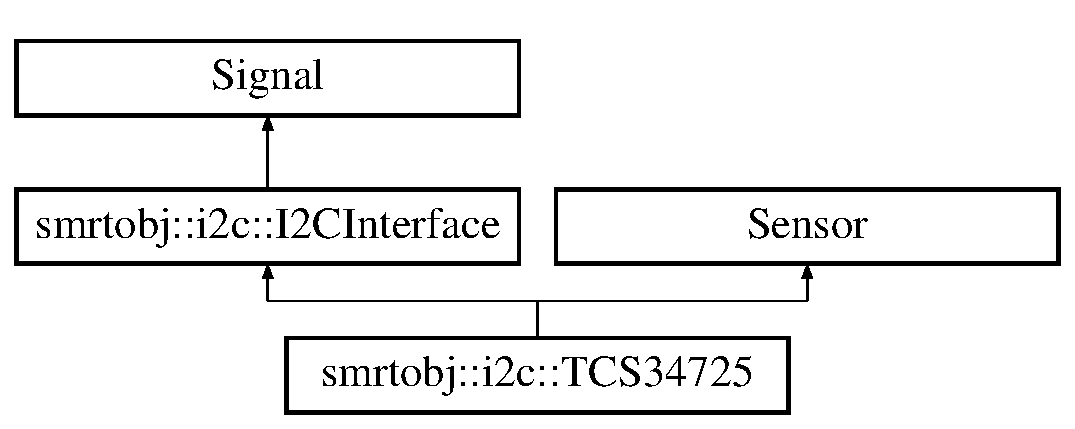
\includegraphics[height=3.000000cm]{classsmrtobj_1_1i2c_1_1_t_c_s34725}
\end{center}
\end{figure}
\subsection*{Public Types}
\begin{DoxyCompactItemize}
\item 
enum \hyperlink{classsmrtobj_1_1i2c_1_1_t_c_s34725_a3e9fb576b01f6e971eab29fce6f1eaf6}{\+\_\+address} \{ \\*
\hyperlink{classsmrtobj_1_1i2c_1_1_t_c_s34725_a3e9fb576b01f6e971eab29fce6f1eaf6afc87724bc312820afc9c6d7194547398}{C\+M\+D\+\_\+\+B\+I\+T\+S} = 0x\+A0, 
\hyperlink{classsmrtobj_1_1i2c_1_1_t_c_s34725_a3e9fb576b01f6e971eab29fce6f1eaf6a7c37bc676673dc9746e11f09c29c019d}{E\+N\+A\+B\+L\+E\+\_\+\+A\+D\+D\+R} = 0x00, 
\hyperlink{classsmrtobj_1_1i2c_1_1_t_c_s34725_a3e9fb576b01f6e971eab29fce6f1eaf6a4838881d8370e155795e73274151f523}{A\+T\+I\+M\+E\+\_\+\+A\+D\+D\+R} = 0x01, 
\hyperlink{classsmrtobj_1_1i2c_1_1_t_c_s34725_a3e9fb576b01f6e971eab29fce6f1eaf6a289dd1778b982779406dea50a93e666b}{W\+T\+I\+M\+E\+\_\+\+A\+D\+D\+R} = 0x03, 
\\*
\hyperlink{classsmrtobj_1_1i2c_1_1_t_c_s34725_a3e9fb576b01f6e971eab29fce6f1eaf6a2e1a0e4542fb8c5b617ff291fbb465e8}{C\+O\+N\+F\+I\+G\+\_\+\+A\+D\+D\+R} = 0x0\+D, 
\hyperlink{classsmrtobj_1_1i2c_1_1_t_c_s34725_a3e9fb576b01f6e971eab29fce6f1eaf6ab9287519f127820154ba097132f4ecce}{C\+O\+N\+T\+R\+O\+L\+\_\+\+A\+D\+D\+R} = 0x0\+F, 
\hyperlink{classsmrtobj_1_1i2c_1_1_t_c_s34725_a3e9fb576b01f6e971eab29fce6f1eaf6ad9ab2d4f773cdd8dc6fbf12af43b3fe8}{I\+D\+\_\+\+A\+D\+D\+R} = 0x12, 
\hyperlink{classsmrtobj_1_1i2c_1_1_t_c_s34725_a3e9fb576b01f6e971eab29fce6f1eaf6ac1bf92f1aa8fe6758b4a7f68b578df69}{C\+O\+L\+O\+R\+\_\+\+A\+D\+D\+R} = 0x14
 \}
\item 
enum \hyperlink{classsmrtobj_1_1i2c_1_1_t_c_s34725_a499caf2237b9c2d6bb988068304ddb33}{\+\_\+values} \{ \\*
\hyperlink{classsmrtobj_1_1i2c_1_1_t_c_s34725_a499caf2237b9c2d6bb988068304ddb33a3791106d9502371e702776a9206e5b5e}{E\+N\+A\+B\+L\+E\+\_\+\+V\+A\+L\+U\+E} = 0x0\+B, 
\hyperlink{classsmrtobj_1_1i2c_1_1_t_c_s34725_a499caf2237b9c2d6bb988068304ddb33a154867d82d6211c5c9833aa9ba677b3d}{C\+O\+N\+T\+R\+O\+L\+\_\+\+V\+A\+L\+U\+E} = 0x01, 
\hyperlink{classsmrtobj_1_1i2c_1_1_t_c_s34725_a499caf2237b9c2d6bb988068304ddb33a43dda57bbe19ab75cada9c969de29da3}{A\+T\+I\+M\+E\+\_\+\+V\+A\+L\+U\+E} = 0x\+C0, 
\hyperlink{classsmrtobj_1_1i2c_1_1_t_c_s34725_a499caf2237b9c2d6bb988068304ddb33a1341c86e1f194c4008f91038d10d08be}{W\+A\+I\+T\+\_\+\+T\+I\+M\+E\+\_\+\+V\+A\+L\+U\+E} = 0x53, 
\\*
\hyperlink{classsmrtobj_1_1i2c_1_1_t_c_s34725_a499caf2237b9c2d6bb988068304ddb33a03d2388f75dbc1cb77739cd253780c52}{R\+\_\+\+C\+O\+E\+F\+F} = 136, 
\hyperlink{classsmrtobj_1_1i2c_1_1_t_c_s34725_a499caf2237b9c2d6bb988068304ddb33ae803725dca1ff4628e19bee7ff83e48e}{G\+\_\+\+C\+O\+E\+F\+F} = 1000, 
\hyperlink{classsmrtobj_1_1i2c_1_1_t_c_s34725_a499caf2237b9c2d6bb988068304ddb33a5320fa41a55331b492e0f3befab0a9a2}{B\+\_\+\+C\+O\+E\+F\+F} = -\/444, 
\hyperlink{classsmrtobj_1_1i2c_1_1_t_c_s34725_a499caf2237b9c2d6bb988068304ddb33af5cf1d7375980b9a41acd5f117331be0}{C\+P\+L} = 497
 \}
\end{DoxyCompactItemize}
\subsection*{Public Member Functions}
\begin{DoxyCompactItemize}
\item 
\hyperlink{classsmrtobj_1_1i2c_1_1_t_c_s34725_a93b35e7535650d4cc3fe256f1e4476c6}{T\+C\+S34725} ()
\item 
\hyperlink{classsmrtobj_1_1i2c_1_1_t_c_s34725_acd2fd6356b8be9598e26d1fbf8550577}{T\+C\+S34725} (const \hyperlink{classsmrtobj_1_1i2c_1_1_t_c_s34725}{T\+C\+S34725} \&s)
\item 
virtual \hyperlink{classsmrtobj_1_1i2c_1_1_t_c_s34725_a4d195655be451fe5b8a5abd233af6f42}{$\sim$\+T\+C\+S34725} ()
\item 
\hyperlink{classsmrtobj_1_1i2c_1_1_t_c_s34725}{T\+C\+S34725} \& \hyperlink{classsmrtobj_1_1i2c_1_1_t_c_s34725_a9360d2d145664e2724a449b05aa21d7a}{operator=} (const \hyperlink{classsmrtobj_1_1i2c_1_1_t_c_s34725}{T\+C\+S34725} \&s)
\item 
virtual bool \hyperlink{classsmrtobj_1_1i2c_1_1_t_c_s34725_af9018c2f326e228d998866692393090f}{is\+Connected} ()
\item 
virtual bool \hyperlink{classsmrtobj_1_1i2c_1_1_t_c_s34725_ace72ff801097ec771026acd605de2d53}{initialize} ()
\item 
virtual bool \hyperlink{classsmrtobj_1_1i2c_1_1_t_c_s34725_ae00be04f529c449287ac9329df3cb7a7}{read} ()
\item 
virtual float \hyperlink{classsmrtobj_1_1i2c_1_1_t_c_s34725_a4318a15406a82e2ccfe9624653e4f37a}{measure} ()
\item 
uint16\+\_\+t \hyperlink{classsmrtobj_1_1i2c_1_1_t_c_s34725_a2ac58333faa1b9f8aea4614c11e7229f}{clear\+\_\+color} ()
\item 
uint16\+\_\+t \hyperlink{classsmrtobj_1_1i2c_1_1_t_c_s34725_aea6fa83010c4f2f476e7917db3b64b17}{red\+\_\+color} ()
\item 
uint16\+\_\+t \hyperlink{classsmrtobj_1_1i2c_1_1_t_c_s34725_a7369ef26040b99b27b981de1aa2f38e2}{green\+\_\+color} ()
\item 
uint16\+\_\+t \hyperlink{classsmrtobj_1_1i2c_1_1_t_c_s34725_a30ee968bf672b9ea3f019dd1046001f0}{blue\+\_\+color} ()
\end{DoxyCompactItemize}
\subsection*{Static Public Attributes}
\begin{DoxyCompactItemize}
\item 
\hypertarget{classsmrtobj_1_1i2c_1_1_t_c_s34725_afb6d3e6f4aed5558a246351db358a9da}{}static const uint8\+\_\+t \hyperlink{classsmrtobj_1_1i2c_1_1_t_c_s34725_afb6d3e6f4aed5558a246351db358a9da}{D\+E\+V\+I\+C\+E\+\_\+\+A\+D\+D\+R\+E\+S\+S} = 0x29\label{classsmrtobj_1_1i2c_1_1_t_c_s34725_afb6d3e6f4aed5558a246351db358a9da}

\begin{DoxyCompactList}\small\item\em Device address (slave) \end{DoxyCompactList}\end{DoxyCompactItemize}
\subsection*{Additional Inherited Members}


\subsection{Detailed Description}
Class \hyperlink{classsmrtobj_1_1i2c_1_1_t_c_s34725}{T\+C\+S34725} models the T\+A\+O\+S \hyperlink{classsmrtobj_1_1i2c_1_1_t_c_s34725}{T\+C\+S34725} color light-\/to-\/digital converter with I\+R filter. The T\+C\+S3472 device provides a digital return of red, green, blue (R\+G\+B), and clear light sensing values. An I\+R blocking filter, integrated on-\/chip and localized to the color sensing photodiodes, minimizes the I\+R spectral component of the incoming light and allows color measurements to be made accurately.

The T\+C\+S3472 is controlled and monitored by data registers and a command register accessed through the serial interface. These registers provide for a variety of control functions and can be read to determine results of the A\+D\+C conversions. 

Definition at line 29 of file T\+C\+S34725.\+h.



\subsection{Member Enumeration Documentation}
\hypertarget{classsmrtobj_1_1i2c_1_1_t_c_s34725_a3e9fb576b01f6e971eab29fce6f1eaf6}{}\index{smrtobj\+::i2c\+::\+T\+C\+S34725@{smrtobj\+::i2c\+::\+T\+C\+S34725}!\+\_\+address@{\+\_\+address}}
\index{\+\_\+address@{\+\_\+address}!smrtobj\+::i2c\+::\+T\+C\+S34725@{smrtobj\+::i2c\+::\+T\+C\+S34725}}
\subsubsection[{\+\_\+address}]{\setlength{\rightskip}{0pt plus 5cm}enum {\bf smrtobj\+::i2c\+::\+T\+C\+S34725\+::\+\_\+address}}\label{classsmrtobj_1_1i2c_1_1_t_c_s34725_a3e9fb576b01f6e971eab29fce6f1eaf6}
Register addresses \begin{Desc}
\item[Enumerator]\par
\begin{description}
\index{C\+M\+D\+\_\+\+B\+I\+T\+S@{C\+M\+D\+\_\+\+B\+I\+T\+S}!smrtobj\+::i2c\+::\+T\+C\+S34725@{smrtobj\+::i2c\+::\+T\+C\+S34725}}\index{smrtobj\+::i2c\+::\+T\+C\+S34725@{smrtobj\+::i2c\+::\+T\+C\+S34725}!C\+M\+D\+\_\+\+B\+I\+T\+S@{C\+M\+D\+\_\+\+B\+I\+T\+S}}\item[{\em 
\hypertarget{classsmrtobj_1_1i2c_1_1_t_c_s34725_a3e9fb576b01f6e971eab29fce6f1eaf6afc87724bc312820afc9c6d7194547398}{}C\+M\+D\+\_\+\+B\+I\+T\+S\label{classsmrtobj_1_1i2c_1_1_t_c_s34725_a3e9fb576b01f6e971eab29fce6f1eaf6afc87724bc312820afc9c6d7194547398}
}]Specifies register address\+: 7th bit to 1 for command and 6th and 5th bits to 01 for auto-\/increment protocol transaction. \index{E\+N\+A\+B\+L\+E\+\_\+\+A\+D\+D\+R@{E\+N\+A\+B\+L\+E\+\_\+\+A\+D\+D\+R}!smrtobj\+::i2c\+::\+T\+C\+S34725@{smrtobj\+::i2c\+::\+T\+C\+S34725}}\index{smrtobj\+::i2c\+::\+T\+C\+S34725@{smrtobj\+::i2c\+::\+T\+C\+S34725}!E\+N\+A\+B\+L\+E\+\_\+\+A\+D\+D\+R@{E\+N\+A\+B\+L\+E\+\_\+\+A\+D\+D\+R}}\item[{\em 
\hypertarget{classsmrtobj_1_1i2c_1_1_t_c_s34725_a3e9fb576b01f6e971eab29fce6f1eaf6a7c37bc676673dc9746e11f09c29c019d}{}E\+N\+A\+B\+L\+E\+\_\+\+A\+D\+D\+R\label{classsmrtobj_1_1i2c_1_1_t_c_s34725_a3e9fb576b01f6e971eab29fce6f1eaf6a7c37bc676673dc9746e11f09c29c019d}
}]Enables states and interrupts. \index{A\+T\+I\+M\+E\+\_\+\+A\+D\+D\+R@{A\+T\+I\+M\+E\+\_\+\+A\+D\+D\+R}!smrtobj\+::i2c\+::\+T\+C\+S34725@{smrtobj\+::i2c\+::\+T\+C\+S34725}}\index{smrtobj\+::i2c\+::\+T\+C\+S34725@{smrtobj\+::i2c\+::\+T\+C\+S34725}!A\+T\+I\+M\+E\+\_\+\+A\+D\+D\+R@{A\+T\+I\+M\+E\+\_\+\+A\+D\+D\+R}}\item[{\em 
\hypertarget{classsmrtobj_1_1i2c_1_1_t_c_s34725_a3e9fb576b01f6e971eab29fce6f1eaf6a4838881d8370e155795e73274151f523}{}A\+T\+I\+M\+E\+\_\+\+A\+D\+D\+R\label{classsmrtobj_1_1i2c_1_1_t_c_s34725_a3e9fb576b01f6e971eab29fce6f1eaf6a4838881d8370e155795e73274151f523}
}]R\+G\+B\+C time. \index{W\+T\+I\+M\+E\+\_\+\+A\+D\+D\+R@{W\+T\+I\+M\+E\+\_\+\+A\+D\+D\+R}!smrtobj\+::i2c\+::\+T\+C\+S34725@{smrtobj\+::i2c\+::\+T\+C\+S34725}}\index{smrtobj\+::i2c\+::\+T\+C\+S34725@{smrtobj\+::i2c\+::\+T\+C\+S34725}!W\+T\+I\+M\+E\+\_\+\+A\+D\+D\+R@{W\+T\+I\+M\+E\+\_\+\+A\+D\+D\+R}}\item[{\em 
\hypertarget{classsmrtobj_1_1i2c_1_1_t_c_s34725_a3e9fb576b01f6e971eab29fce6f1eaf6a289dd1778b982779406dea50a93e666b}{}W\+T\+I\+M\+E\+\_\+\+A\+D\+D\+R\label{classsmrtobj_1_1i2c_1_1_t_c_s34725_a3e9fb576b01f6e971eab29fce6f1eaf6a289dd1778b982779406dea50a93e666b}
}]Wait time. \index{C\+O\+N\+F\+I\+G\+\_\+\+A\+D\+D\+R@{C\+O\+N\+F\+I\+G\+\_\+\+A\+D\+D\+R}!smrtobj\+::i2c\+::\+T\+C\+S34725@{smrtobj\+::i2c\+::\+T\+C\+S34725}}\index{smrtobj\+::i2c\+::\+T\+C\+S34725@{smrtobj\+::i2c\+::\+T\+C\+S34725}!C\+O\+N\+F\+I\+G\+\_\+\+A\+D\+D\+R@{C\+O\+N\+F\+I\+G\+\_\+\+A\+D\+D\+R}}\item[{\em 
\hypertarget{classsmrtobj_1_1i2c_1_1_t_c_s34725_a3e9fb576b01f6e971eab29fce6f1eaf6a2e1a0e4542fb8c5b617ff291fbb465e8}{}C\+O\+N\+F\+I\+G\+\_\+\+A\+D\+D\+R\label{classsmrtobj_1_1i2c_1_1_t_c_s34725_a3e9fb576b01f6e971eab29fce6f1eaf6a2e1a0e4542fb8c5b617ff291fbb465e8}
}]Configuration. \index{C\+O\+N\+T\+R\+O\+L\+\_\+\+A\+D\+D\+R@{C\+O\+N\+T\+R\+O\+L\+\_\+\+A\+D\+D\+R}!smrtobj\+::i2c\+::\+T\+C\+S34725@{smrtobj\+::i2c\+::\+T\+C\+S34725}}\index{smrtobj\+::i2c\+::\+T\+C\+S34725@{smrtobj\+::i2c\+::\+T\+C\+S34725}!C\+O\+N\+T\+R\+O\+L\+\_\+\+A\+D\+D\+R@{C\+O\+N\+T\+R\+O\+L\+\_\+\+A\+D\+D\+R}}\item[{\em 
\hypertarget{classsmrtobj_1_1i2c_1_1_t_c_s34725_a3e9fb576b01f6e971eab29fce6f1eaf6ab9287519f127820154ba097132f4ecce}{}C\+O\+N\+T\+R\+O\+L\+\_\+\+A\+D\+D\+R\label{classsmrtobj_1_1i2c_1_1_t_c_s34725_a3e9fb576b01f6e971eab29fce6f1eaf6ab9287519f127820154ba097132f4ecce}
}]Control. \index{I\+D\+\_\+\+A\+D\+D\+R@{I\+D\+\_\+\+A\+D\+D\+R}!smrtobj\+::i2c\+::\+T\+C\+S34725@{smrtobj\+::i2c\+::\+T\+C\+S34725}}\index{smrtobj\+::i2c\+::\+T\+C\+S34725@{smrtobj\+::i2c\+::\+T\+C\+S34725}!I\+D\+\_\+\+A\+D\+D\+R@{I\+D\+\_\+\+A\+D\+D\+R}}\item[{\em 
\hypertarget{classsmrtobj_1_1i2c_1_1_t_c_s34725_a3e9fb576b01f6e971eab29fce6f1eaf6ad9ab2d4f773cdd8dc6fbf12af43b3fe8}{}I\+D\+\_\+\+A\+D\+D\+R\label{classsmrtobj_1_1i2c_1_1_t_c_s34725_a3e9fb576b01f6e971eab29fce6f1eaf6ad9ab2d4f773cdd8dc6fbf12af43b3fe8}
}]Device I\+D. \index{C\+O\+L\+O\+R\+\_\+\+A\+D\+D\+R@{C\+O\+L\+O\+R\+\_\+\+A\+D\+D\+R}!smrtobj\+::i2c\+::\+T\+C\+S34725@{smrtobj\+::i2c\+::\+T\+C\+S34725}}\index{smrtobj\+::i2c\+::\+T\+C\+S34725@{smrtobj\+::i2c\+::\+T\+C\+S34725}!C\+O\+L\+O\+R\+\_\+\+A\+D\+D\+R@{C\+O\+L\+O\+R\+\_\+\+A\+D\+D\+R}}\item[{\em 
\hypertarget{classsmrtobj_1_1i2c_1_1_t_c_s34725_a3e9fb576b01f6e971eab29fce6f1eaf6ac1bf92f1aa8fe6758b4a7f68b578df69}{}C\+O\+L\+O\+R\+\_\+\+A\+D\+D\+R\label{classsmrtobj_1_1i2c_1_1_t_c_s34725_a3e9fb576b01f6e971eab29fce6f1eaf6ac1bf92f1aa8fe6758b4a7f68b578df69}
}]Color address. \end{description}
\end{Desc}


Definition at line 38 of file T\+C\+S34725.\+h.

\hypertarget{classsmrtobj_1_1i2c_1_1_t_c_s34725_a499caf2237b9c2d6bb988068304ddb33}{}\index{smrtobj\+::i2c\+::\+T\+C\+S34725@{smrtobj\+::i2c\+::\+T\+C\+S34725}!\+\_\+values@{\+\_\+values}}
\index{\+\_\+values@{\+\_\+values}!smrtobj\+::i2c\+::\+T\+C\+S34725@{smrtobj\+::i2c\+::\+T\+C\+S34725}}
\subsubsection[{\+\_\+values}]{\setlength{\rightskip}{0pt plus 5cm}enum {\bf smrtobj\+::i2c\+::\+T\+C\+S34725\+::\+\_\+values}}\label{classsmrtobj_1_1i2c_1_1_t_c_s34725_a499caf2237b9c2d6bb988068304ddb33}
Command values \begin{Desc}
\item[Enumerator]\par
\begin{description}
\index{E\+N\+A\+B\+L\+E\+\_\+\+V\+A\+L\+U\+E@{E\+N\+A\+B\+L\+E\+\_\+\+V\+A\+L\+U\+E}!smrtobj\+::i2c\+::\+T\+C\+S34725@{smrtobj\+::i2c\+::\+T\+C\+S34725}}\index{smrtobj\+::i2c\+::\+T\+C\+S34725@{smrtobj\+::i2c\+::\+T\+C\+S34725}!E\+N\+A\+B\+L\+E\+\_\+\+V\+A\+L\+U\+E@{E\+N\+A\+B\+L\+E\+\_\+\+V\+A\+L\+U\+E}}\item[{\em 
\hypertarget{classsmrtobj_1_1i2c_1_1_t_c_s34725_a499caf2237b9c2d6bb988068304ddb33a3791106d9502371e702776a9206e5b5e}{}E\+N\+A\+B\+L\+E\+\_\+\+V\+A\+L\+U\+E\label{classsmrtobj_1_1i2c_1_1_t_c_s34725_a499caf2237b9c2d6bb988068304ddb33a3791106d9502371e702776a9206e5b5e}
}]Enable\+: sets P\+O\+N (bit 0) and A\+E\+N (bit 1) to 1 enable wait, W\+E\+N (bit 3) to 1 disable interrupt, A\+I\+E\+N (bit 4) to 0. \index{C\+O\+N\+T\+R\+O\+L\+\_\+\+V\+A\+L\+U\+E@{C\+O\+N\+T\+R\+O\+L\+\_\+\+V\+A\+L\+U\+E}!smrtobj\+::i2c\+::\+T\+C\+S34725@{smrtobj\+::i2c\+::\+T\+C\+S34725}}\index{smrtobj\+::i2c\+::\+T\+C\+S34725@{smrtobj\+::i2c\+::\+T\+C\+S34725}!C\+O\+N\+T\+R\+O\+L\+\_\+\+V\+A\+L\+U\+E@{C\+O\+N\+T\+R\+O\+L\+\_\+\+V\+A\+L\+U\+E}}\item[{\em 
\hypertarget{classsmrtobj_1_1i2c_1_1_t_c_s34725_a499caf2237b9c2d6bb988068304ddb33a154867d82d6211c5c9833aa9ba677b3d}{}C\+O\+N\+T\+R\+O\+L\+\_\+\+V\+A\+L\+U\+E\label{classsmrtobj_1_1i2c_1_1_t_c_s34725_a499caf2237b9c2d6bb988068304ddb33a154867d82d6211c5c9833aa9ba677b3d}
}]Control\+: 0x00 \+: 1 x gain, 0x01 \+: 4 x gain, 0x10 \+: 16 x gain, 0x11 \+: 60 x gain. \index{A\+T\+I\+M\+E\+\_\+\+V\+A\+L\+U\+E@{A\+T\+I\+M\+E\+\_\+\+V\+A\+L\+U\+E}!smrtobj\+::i2c\+::\+T\+C\+S34725@{smrtobj\+::i2c\+::\+T\+C\+S34725}}\index{smrtobj\+::i2c\+::\+T\+C\+S34725@{smrtobj\+::i2c\+::\+T\+C\+S34725}!A\+T\+I\+M\+E\+\_\+\+V\+A\+L\+U\+E@{A\+T\+I\+M\+E\+\_\+\+V\+A\+L\+U\+E}}\item[{\em 
\hypertarget{classsmrtobj_1_1i2c_1_1_t_c_s34725_a499caf2237b9c2d6bb988068304ddb33a43dda57bbe19ab75cada9c969de29da3}{}A\+T\+I\+M\+E\+\_\+\+V\+A\+L\+U\+E\label{classsmrtobj_1_1i2c_1_1_t_c_s34725_a499caf2237b9c2d6bb988068304ddb33a43dda57bbe19ab75cada9c969de29da3}
}]R\+G\+B\+C time\+: 256 -\/ round\+Towards\+Zero( itime / 2.\+4 ); 0x\+F\+F \+: 2.\+4 ms, 0x\+F6 \+: 24 ms, 0x\+D5 \+: 101 ms, 0x\+C0 \+: 154 ms, 0x00 \+: 700 ms. \index{W\+A\+I\+T\+\_\+\+T\+I\+M\+E\+\_\+\+V\+A\+L\+U\+E@{W\+A\+I\+T\+\_\+\+T\+I\+M\+E\+\_\+\+V\+A\+L\+U\+E}!smrtobj\+::i2c\+::\+T\+C\+S34725@{smrtobj\+::i2c\+::\+T\+C\+S34725}}\index{smrtobj\+::i2c\+::\+T\+C\+S34725@{smrtobj\+::i2c\+::\+T\+C\+S34725}!W\+A\+I\+T\+\_\+\+T\+I\+M\+E\+\_\+\+V\+A\+L\+U\+E@{W\+A\+I\+T\+\_\+\+T\+I\+M\+E\+\_\+\+V\+A\+L\+U\+E}}\item[{\em 
\hypertarget{classsmrtobj_1_1i2c_1_1_t_c_s34725_a499caf2237b9c2d6bb988068304ddb33a1341c86e1f194c4008f91038d10d08be}{}W\+A\+I\+T\+\_\+\+T\+I\+M\+E\+\_\+\+V\+A\+L\+U\+E\label{classsmrtobj_1_1i2c_1_1_t_c_s34725_a499caf2237b9c2d6bb988068304ddb33a1341c86e1f194c4008f91038d10d08be}
}]Wait time\+: T=5s \+: 256 -\/ round\+Towards\+Zero( 5000 / 28.\+8 ) = 0x53; T=1s \+: 256 -\/ round\+Towards\+Zero( 5000 / 28.\+8 ) = 0x\+D\+D;. \index{R\+\_\+\+C\+O\+E\+F\+F@{R\+\_\+\+C\+O\+E\+F\+F}!smrtobj\+::i2c\+::\+T\+C\+S34725@{smrtobj\+::i2c\+::\+T\+C\+S34725}}\index{smrtobj\+::i2c\+::\+T\+C\+S34725@{smrtobj\+::i2c\+::\+T\+C\+S34725}!R\+\_\+\+C\+O\+E\+F\+F@{R\+\_\+\+C\+O\+E\+F\+F}}\item[{\em 
\hypertarget{classsmrtobj_1_1i2c_1_1_t_c_s34725_a499caf2237b9c2d6bb988068304ddb33a03d2388f75dbc1cb77739cd253780c52}{}R\+\_\+\+C\+O\+E\+F\+F\label{classsmrtobj_1_1i2c_1_1_t_c_s34725_a499caf2237b9c2d6bb988068304ddb33a03d2388f75dbc1cb77739cd253780c52}
}]Coefficient for red component to convert in L\+U\+X with gain = 1, atime = 154. \index{G\+\_\+\+C\+O\+E\+F\+F@{G\+\_\+\+C\+O\+E\+F\+F}!smrtobj\+::i2c\+::\+T\+C\+S34725@{smrtobj\+::i2c\+::\+T\+C\+S34725}}\index{smrtobj\+::i2c\+::\+T\+C\+S34725@{smrtobj\+::i2c\+::\+T\+C\+S34725}!G\+\_\+\+C\+O\+E\+F\+F@{G\+\_\+\+C\+O\+E\+F\+F}}\item[{\em 
\hypertarget{classsmrtobj_1_1i2c_1_1_t_c_s34725_a499caf2237b9c2d6bb988068304ddb33ae803725dca1ff4628e19bee7ff83e48e}{}G\+\_\+\+C\+O\+E\+F\+F\label{classsmrtobj_1_1i2c_1_1_t_c_s34725_a499caf2237b9c2d6bb988068304ddb33ae803725dca1ff4628e19bee7ff83e48e}
}]Coefficient for green component to convert in L\+U\+X with gain = 1, atime = 154. \index{B\+\_\+\+C\+O\+E\+F\+F@{B\+\_\+\+C\+O\+E\+F\+F}!smrtobj\+::i2c\+::\+T\+C\+S34725@{smrtobj\+::i2c\+::\+T\+C\+S34725}}\index{smrtobj\+::i2c\+::\+T\+C\+S34725@{smrtobj\+::i2c\+::\+T\+C\+S34725}!B\+\_\+\+C\+O\+E\+F\+F@{B\+\_\+\+C\+O\+E\+F\+F}}\item[{\em 
\hypertarget{classsmrtobj_1_1i2c_1_1_t_c_s34725_a499caf2237b9c2d6bb988068304ddb33a5320fa41a55331b492e0f3befab0a9a2}{}B\+\_\+\+C\+O\+E\+F\+F\label{classsmrtobj_1_1i2c_1_1_t_c_s34725_a499caf2237b9c2d6bb988068304ddb33a5320fa41a55331b492e0f3befab0a9a2}
}]Coefficient for blie component to convert in L\+U\+X with gain = 1, atime = 154. \index{C\+P\+L@{C\+P\+L}!smrtobj\+::i2c\+::\+T\+C\+S34725@{smrtobj\+::i2c\+::\+T\+C\+S34725}}\index{smrtobj\+::i2c\+::\+T\+C\+S34725@{smrtobj\+::i2c\+::\+T\+C\+S34725}!C\+P\+L@{C\+P\+L}}\item[{\em 
\hypertarget{classsmrtobj_1_1i2c_1_1_t_c_s34725_a499caf2237b9c2d6bb988068304ddb33af5cf1d7375980b9a41acd5f117331be0}{}C\+P\+L\label{classsmrtobj_1_1i2c_1_1_t_c_s34725_a499caf2237b9c2d6bb988068304ddb33af5cf1d7375980b9a41acd5f117331be0}
}]Coefficient to convert in L\+U\+X with gain = 1, atime = 154. \end{description}
\end{Desc}


Definition at line 67 of file T\+C\+S34725.\+h.



\subsection{Constructor \& Destructor Documentation}
\hypertarget{classsmrtobj_1_1i2c_1_1_t_c_s34725_a93b35e7535650d4cc3fe256f1e4476c6}{}\index{smrtobj\+::i2c\+::\+T\+C\+S34725@{smrtobj\+::i2c\+::\+T\+C\+S34725}!T\+C\+S34725@{T\+C\+S34725}}
\index{T\+C\+S34725@{T\+C\+S34725}!smrtobj\+::i2c\+::\+T\+C\+S34725@{smrtobj\+::i2c\+::\+T\+C\+S34725}}
\subsubsection[{T\+C\+S34725()}]{\setlength{\rightskip}{0pt plus 5cm}smrtobj\+::\+T\+C\+S34725\+::\+T\+C\+S34725 (
\begin{DoxyParamCaption}
{}
\end{DoxyParamCaption}
)}\label{classsmrtobj_1_1i2c_1_1_t_c_s34725_a93b35e7535650d4cc3fe256f1e4476c6}
Default Constructor. Sets the device address. 

Definition at line 14 of file T\+C\+S34725.\+cpp.

\hypertarget{classsmrtobj_1_1i2c_1_1_t_c_s34725_acd2fd6356b8be9598e26d1fbf8550577}{}\index{smrtobj\+::i2c\+::\+T\+C\+S34725@{smrtobj\+::i2c\+::\+T\+C\+S34725}!T\+C\+S34725@{T\+C\+S34725}}
\index{T\+C\+S34725@{T\+C\+S34725}!smrtobj\+::i2c\+::\+T\+C\+S34725@{smrtobj\+::i2c\+::\+T\+C\+S34725}}
\subsubsection[{T\+C\+S34725(const T\+C\+S34725 \&s)}]{\setlength{\rightskip}{0pt plus 5cm}smrtobj\+::\+T\+C\+S34725\+::\+T\+C\+S34725 (
\begin{DoxyParamCaption}
\item[{const {\bf T\+C\+S34725} \&}]{s}
\end{DoxyParamCaption}
)}\label{classsmrtobj_1_1i2c_1_1_t_c_s34725_acd2fd6356b8be9598e26d1fbf8550577}
Copy Constructor.


\begin{DoxyParams}[1]{Parameters}
\mbox{\tt in}  & {\em s} & i2c sensor object \\
\hline
\end{DoxyParams}


Definition at line 22 of file T\+C\+S34725.\+cpp.

\hypertarget{classsmrtobj_1_1i2c_1_1_t_c_s34725_a4d195655be451fe5b8a5abd233af6f42}{}\index{smrtobj\+::i2c\+::\+T\+C\+S34725@{smrtobj\+::i2c\+::\+T\+C\+S34725}!````~T\+C\+S34725@{$\sim$\+T\+C\+S34725}}
\index{````~T\+C\+S34725@{$\sim$\+T\+C\+S34725}!smrtobj\+::i2c\+::\+T\+C\+S34725@{smrtobj\+::i2c\+::\+T\+C\+S34725}}
\subsubsection[{$\sim$\+T\+C\+S34725()}]{\setlength{\rightskip}{0pt plus 5cm}smrtobj\+::\+T\+C\+S34725\+::$\sim$\+T\+C\+S34725 (
\begin{DoxyParamCaption}
{}
\end{DoxyParamCaption}
)\hspace{0.3cm}{\ttfamily [virtual]}}\label{classsmrtobj_1_1i2c_1_1_t_c_s34725_a4d195655be451fe5b8a5abd233af6f42}
Destructor. 

Definition at line 18 of file T\+C\+S34725.\+cpp.



\subsection{Member Function Documentation}
\hypertarget{classsmrtobj_1_1i2c_1_1_t_c_s34725_a30ee968bf672b9ea3f019dd1046001f0}{}\index{smrtobj\+::i2c\+::\+T\+C\+S34725@{smrtobj\+::i2c\+::\+T\+C\+S34725}!blue\+\_\+color@{blue\+\_\+color}}
\index{blue\+\_\+color@{blue\+\_\+color}!smrtobj\+::i2c\+::\+T\+C\+S34725@{smrtobj\+::i2c\+::\+T\+C\+S34725}}
\subsubsection[{blue\+\_\+color()}]{\setlength{\rightskip}{0pt plus 5cm}uint16\+\_\+t smrtobj\+::i2c\+::\+T\+C\+S34725\+::blue\+\_\+color (
\begin{DoxyParamCaption}
{}
\end{DoxyParamCaption}
)\hspace{0.3cm}{\ttfamily [inline]}}\label{classsmrtobj_1_1i2c_1_1_t_c_s34725_a30ee968bf672b9ea3f019dd1046001f0}
Returns the blue component of the last sensor reading.

\begin{DoxyReturn}{Returns}
blue component 
\end{DoxyReturn}


Definition at line 200 of file T\+C\+S34725.\+h.

\hypertarget{classsmrtobj_1_1i2c_1_1_t_c_s34725_a2ac58333faa1b9f8aea4614c11e7229f}{}\index{smrtobj\+::i2c\+::\+T\+C\+S34725@{smrtobj\+::i2c\+::\+T\+C\+S34725}!clear\+\_\+color@{clear\+\_\+color}}
\index{clear\+\_\+color@{clear\+\_\+color}!smrtobj\+::i2c\+::\+T\+C\+S34725@{smrtobj\+::i2c\+::\+T\+C\+S34725}}
\subsubsection[{clear\+\_\+color()}]{\setlength{\rightskip}{0pt plus 5cm}uint16\+\_\+t smrtobj\+::i2c\+::\+T\+C\+S34725\+::clear\+\_\+color (
\begin{DoxyParamCaption}
{}
\end{DoxyParamCaption}
)\hspace{0.3cm}{\ttfamily [inline]}}\label{classsmrtobj_1_1i2c_1_1_t_c_s34725_a2ac58333faa1b9f8aea4614c11e7229f}
Returns the clear component of the last sensor reading.

\begin{DoxyReturn}{Returns}
clear component 
\end{DoxyReturn}


Definition at line 179 of file T\+C\+S34725.\+h.

\hypertarget{classsmrtobj_1_1i2c_1_1_t_c_s34725_a7369ef26040b99b27b981de1aa2f38e2}{}\index{smrtobj\+::i2c\+::\+T\+C\+S34725@{smrtobj\+::i2c\+::\+T\+C\+S34725}!green\+\_\+color@{green\+\_\+color}}
\index{green\+\_\+color@{green\+\_\+color}!smrtobj\+::i2c\+::\+T\+C\+S34725@{smrtobj\+::i2c\+::\+T\+C\+S34725}}
\subsubsection[{green\+\_\+color()}]{\setlength{\rightskip}{0pt plus 5cm}uint16\+\_\+t smrtobj\+::i2c\+::\+T\+C\+S34725\+::green\+\_\+color (
\begin{DoxyParamCaption}
{}
\end{DoxyParamCaption}
)\hspace{0.3cm}{\ttfamily [inline]}}\label{classsmrtobj_1_1i2c_1_1_t_c_s34725_a7369ef26040b99b27b981de1aa2f38e2}
Returns the green component of the last sensor reading.

\begin{DoxyReturn}{Returns}
green component 
\end{DoxyReturn}


Definition at line 193 of file T\+C\+S34725.\+h.

\hypertarget{classsmrtobj_1_1i2c_1_1_t_c_s34725_ace72ff801097ec771026acd605de2d53}{}\index{smrtobj\+::i2c\+::\+T\+C\+S34725@{smrtobj\+::i2c\+::\+T\+C\+S34725}!initialize@{initialize}}
\index{initialize@{initialize}!smrtobj\+::i2c\+::\+T\+C\+S34725@{smrtobj\+::i2c\+::\+T\+C\+S34725}}
\subsubsection[{initialize()}]{\setlength{\rightskip}{0pt plus 5cm}bool smrtobj\+::\+T\+C\+S34725\+::initialize (
\begin{DoxyParamCaption}
{}
\end{DoxyParamCaption}
)\hspace{0.3cm}{\ttfamily [virtual]}}\label{classsmrtobj_1_1i2c_1_1_t_c_s34725_ace72ff801097ec771026acd605de2d53}
Initializes the i2c device\+: power on and prepare for general usage. This function sets up the {\itshape A\+T\+I\+M\+E}, {\itshape W\+T\+I\+M\+E}, {\itshape Gain} Control and {\itshape A\+Ds} {\itshape and} {\itshape oscillator} values defined in \hyperlink{classsmrtobj_1_1i2c_1_1_t_c_s34725_a499caf2237b9c2d6bb988068304ddb33}{smrtobj\+::i2c\+::\+T\+C\+S34725\+::\+\_\+values}.

\begin{DoxyReturn}{Returns}
true for success, or false if any error occurs. 
\end{DoxyReturn}


Implements \hyperlink{classsmrtobj_1_1i2c_1_1_i2_c_interface_a4ff1ff083d877c7c0816299b11965eb4}{smrtobj\+::i2c\+::\+I2\+C\+Interface}.



Definition at line 48 of file T\+C\+S34725.\+cpp.

\hypertarget{classsmrtobj_1_1i2c_1_1_t_c_s34725_af9018c2f326e228d998866692393090f}{}\index{smrtobj\+::i2c\+::\+T\+C\+S34725@{smrtobj\+::i2c\+::\+T\+C\+S34725}!is\+Connected@{is\+Connected}}
\index{is\+Connected@{is\+Connected}!smrtobj\+::i2c\+::\+T\+C\+S34725@{smrtobj\+::i2c\+::\+T\+C\+S34725}}
\subsubsection[{is\+Connected()}]{\setlength{\rightskip}{0pt plus 5cm}bool smrtobj\+::\+T\+C\+S34725\+::is\+Connected (
\begin{DoxyParamCaption}
{}
\end{DoxyParamCaption}
)\hspace{0.3cm}{\ttfamily [virtual]}}\label{classsmrtobj_1_1i2c_1_1_t_c_s34725_af9018c2f326e228d998866692393090f}
Tests if the device is connected. Make sure the device is connected and responds as expected.

\begin{DoxyReturn}{Returns}
true if connection is valid, false otherwise 
\end{DoxyReturn}


Implements \hyperlink{classsmrtobj_1_1i2c_1_1_i2_c_interface_a33fd37bafaf8c7e8184acb6470322bce}{smrtobj\+::i2c\+::\+I2\+C\+Interface}.



Definition at line 90 of file T\+C\+S34725.\+cpp.

\hypertarget{classsmrtobj_1_1i2c_1_1_t_c_s34725_a4318a15406a82e2ccfe9624653e4f37a}{}\index{smrtobj\+::i2c\+::\+T\+C\+S34725@{smrtobj\+::i2c\+::\+T\+C\+S34725}!measure@{measure}}
\index{measure@{measure}!smrtobj\+::i2c\+::\+T\+C\+S34725@{smrtobj\+::i2c\+::\+T\+C\+S34725}}
\subsubsection[{measure()}]{\setlength{\rightskip}{0pt plus 5cm}float smrtobj\+::\+T\+C\+S34725\+::measure (
\begin{DoxyParamCaption}
{}
\end{DoxyParamCaption}
)\hspace{0.3cm}{\ttfamily [virtual]}}\label{classsmrtobj_1_1i2c_1_1_t_c_s34725_a4318a15406a82e2ccfe9624653e4f37a}
Converts components in Lux value.


\begin{DoxyCode}
\textcolor{keywordtype}{float} ir = ( ( red + green + blue - clear ) / 2 );
\textcolor{keywordtype}{float} lux = ( \hyperlink{classsmrtobj_1_1i2c_1_1_t_c_s34725_a499caf2237b9c2d6bb988068304ddb33a03d2388f75dbc1cb77739cd253780c52}{R\_COEFF} * ( red - ir) + \hyperlink{classsmrtobj_1_1i2c_1_1_t_c_s34725_a499caf2237b9c2d6bb988068304ddb33ae803725dca1ff4628e19bee7ff83e48e}{G\_COEFF} * ( green - ir) + 
      \hyperlink{classsmrtobj_1_1i2c_1_1_t_c_s34725_a499caf2237b9c2d6bb988068304ddb33a5320fa41a55331b492e0f3befab0a9a2}{B\_COEFF} * ( blue - ir) ) / \hyperlink{classsmrtobj_1_1i2c_1_1_t_c_s34725_a499caf2237b9c2d6bb988068304ddb33af5cf1d7375980b9a41acd5f117331be0}{CPL};
\end{DoxyCode}


\begin{DoxyReturn}{Returns}
value in Lux 
\end{DoxyReturn}


Definition at line 120 of file T\+C\+S34725.\+cpp.

\hypertarget{classsmrtobj_1_1i2c_1_1_t_c_s34725_a9360d2d145664e2724a449b05aa21d7a}{}\index{smrtobj\+::i2c\+::\+T\+C\+S34725@{smrtobj\+::i2c\+::\+T\+C\+S34725}!operator=@{operator=}}
\index{operator=@{operator=}!smrtobj\+::i2c\+::\+T\+C\+S34725@{smrtobj\+::i2c\+::\+T\+C\+S34725}}
\subsubsection[{operator=(const T\+C\+S34725 \&s)}]{\setlength{\rightskip}{0pt plus 5cm}{\bf T\+C\+S34725} \& smrtobj\+::\+T\+C\+S34725\+::operator= (
\begin{DoxyParamCaption}
\item[{const {\bf T\+C\+S34725} \&}]{s}
\end{DoxyParamCaption}
)}\label{classsmrtobj_1_1i2c_1_1_t_c_s34725_a9360d2d145664e2724a449b05aa21d7a}
Override operator =


\begin{DoxyParams}[1]{Parameters}
\mbox{\tt in}  & {\em s} & source signal object\\
\hline
\end{DoxyParams}
\begin{DoxyReturn}{Returns}
destination signal reference 
\end{DoxyReturn}


Definition at line 30 of file T\+C\+S34725.\+cpp.

\hypertarget{classsmrtobj_1_1i2c_1_1_t_c_s34725_ae00be04f529c449287ac9329df3cb7a7}{}\index{smrtobj\+::i2c\+::\+T\+C\+S34725@{smrtobj\+::i2c\+::\+T\+C\+S34725}!read@{read}}
\index{read@{read}!smrtobj\+::i2c\+::\+T\+C\+S34725@{smrtobj\+::i2c\+::\+T\+C\+S34725}}
\subsubsection[{read()}]{\setlength{\rightskip}{0pt plus 5cm}bool smrtobj\+::\+T\+C\+S34725\+::read (
\begin{DoxyParamCaption}
{}
\end{DoxyParamCaption}
)\hspace{0.3cm}{\ttfamily [virtual]}}\label{classsmrtobj_1_1i2c_1_1_t_c_s34725_ae00be04f529c449287ac9329df3cb7a7}
Reads data from the i2c device. This function read 8 byte\+:
\begin{DoxyItemize}
\item 1st byte clear component, (Byte0) is the less significant byte
\item 2nd byte clear component, (Byte1) is the most significant byte
\item 3rd byte red component, (Byte0) is the less significant byte
\item 4th byte red component, (Byte1) is the most significant byte
\item 5th byte green component, (Byte0) is the less significant byte
\item 6th byte green component, (Byte1) is the most significant byte
\item 7th byte blue component, (Byte0) is the less significant byte
\item 8th byte blue component, (Byte1) is the most significant byte
\end{DoxyItemize}

Data is calculate as\+:


\begin{DoxyCode}
value = (Byte1] << 8) | Byte0;
\end{DoxyCode}


The value read is stored into the internal buffer {\itshape m\+\_\+value}.

\begin{DoxyReturn}{Returns}
true for success, or false if any error occurs. 
\end{DoxyReturn}


Implements \hyperlink{classsmrtobj_1_1i2c_1_1_i2_c_interface_a58bc734662a60de6a7cb7976c2179753}{smrtobj\+::i2c\+::\+I2\+C\+Interface}.



Definition at line 105 of file T\+C\+S34725.\+cpp.

\hypertarget{classsmrtobj_1_1i2c_1_1_t_c_s34725_aea6fa83010c4f2f476e7917db3b64b17}{}\index{smrtobj\+::i2c\+::\+T\+C\+S34725@{smrtobj\+::i2c\+::\+T\+C\+S34725}!red\+\_\+color@{red\+\_\+color}}
\index{red\+\_\+color@{red\+\_\+color}!smrtobj\+::i2c\+::\+T\+C\+S34725@{smrtobj\+::i2c\+::\+T\+C\+S34725}}
\subsubsection[{red\+\_\+color()}]{\setlength{\rightskip}{0pt plus 5cm}uint16\+\_\+t smrtobj\+::i2c\+::\+T\+C\+S34725\+::red\+\_\+color (
\begin{DoxyParamCaption}
{}
\end{DoxyParamCaption}
)\hspace{0.3cm}{\ttfamily [inline]}}\label{classsmrtobj_1_1i2c_1_1_t_c_s34725_aea6fa83010c4f2f476e7917db3b64b17}
Returns the red component of the last sensor reading.

\begin{DoxyReturn}{Returns}
red component 
\end{DoxyReturn}


Definition at line 186 of file T\+C\+S34725.\+h.



The documentation for this class was generated from the following files\+:\begin{DoxyCompactItemize}
\item 
libraries/\+Smrt\+Obj\+I2\+C/src/sensors/\hyperlink{_t_c_s34725_8h}{T\+C\+S34725.\+h}\item 
libraries/\+Smrt\+Obj\+I2\+C/src/sensors/\hyperlink{_t_c_s34725_8cpp}{T\+C\+S34725.\+cpp}\end{DoxyCompactItemize}

\chapter{File Documentation}
\hypertarget{avgvalue_8cpp}{}\section{libraries/\+Smrt\+Obj\+Data/src/avgvalue.cpp File Reference}
\label{avgvalue_8cpp}\index{libraries/\+Smrt\+Obj\+Data/src/avgvalue.\+cpp@{libraries/\+Smrt\+Obj\+Data/src/avgvalue.\+cpp}}


Arduino library to calculate cumulative average.  


{\ttfamily \#include \char`\"{}avgvalue.\+h\char`\"{}}\\*


\subsection{Detailed Description}
Arduino library to calculate cumulative average. 

\begin{DoxyAuthor}{Author}
Marco Boeris Frusca 
\end{DoxyAuthor}

\hypertarget{avgvalue_8h}{}\section{libraries/\+Smrt\+Obj\+Data/src/avgvalue.h File Reference}
\label{avgvalue_8h}\index{libraries/\+Smrt\+Obj\+Data/src/avgvalue.\+h@{libraries/\+Smrt\+Obj\+Data/src/avgvalue.\+h}}


Arduino library to calculate cumulative average.  


{\ttfamily \#include \char`\"{}W\+Program.\+h\char`\"{}}\\*
{\ttfamily \#include \char`\"{}pins\+\_\+arduino.\+h\char`\"{}}\\*
\subsection*{Classes}
\begin{DoxyCompactItemize}
\item 
class \hyperlink{classsmrtobj_1_1data_1_1_avg_value}{smrtobj\+::data\+::\+Avg\+Value}
\end{DoxyCompactItemize}


\subsection{Detailed Description}
Arduino library to calculate cumulative average. 

\begin{DoxyAuthor}{Author}
Marco Boeris Frusca 
\end{DoxyAuthor}

\hypertarget{gpsposition_8cpp}{}\section{libraries/\+Smrt\+Obj\+Data/src/gpsposition.cpp File Reference}
\label{gpsposition_8cpp}\index{libraries/\+Smrt\+Obj\+Data/src/gpsposition.\+cpp@{libraries/\+Smrt\+Obj\+Data/src/gpsposition.\+cpp}}


Arduino library to model G\+P\+S position. A coordinate has three component\+: latitude, longitude and altitude. Latitude and longitude are in decimal degree format (where positive value means North for latitude and West for longitude). Altitude value is an integer and its unit is meter.  


{\ttfamily \#include \char`\"{}gpsposition.\+h\char`\"{}}\\*


\subsection{Detailed Description}
Arduino library to model G\+P\+S position. A coordinate has three component\+: latitude, longitude and altitude. Latitude and longitude are in decimal degree format (where positive value means North for latitude and West for longitude). Altitude value is an integer and its unit is meter. 

\begin{DoxyAuthor}{Author}
Marco Boeris Frusca 
\end{DoxyAuthor}

\hypertarget{gpsposition_8h}{}\section{libraries/\+Smrt\+Obj\+Data/src/gpsposition.h File Reference}
\label{gpsposition_8h}\index{libraries/\+Smrt\+Obj\+Data/src/gpsposition.\+h@{libraries/\+Smrt\+Obj\+Data/src/gpsposition.\+h}}


Arduino library to model G\+P\+S position. A coordinate has three component\+: latitude, longitude and altitude. Latitude and longitude are in decimal degree format (where positive value means North for latitude and West for longitude). Altitude value is an integer and its unit is meter.  


{\ttfamily \#include \char`\"{}W\+Program.\+h\char`\"{}}\\*
{\ttfamily \#include \char`\"{}pins\+\_\+arduino.\+h\char`\"{}}\\*
\subsection*{Classes}
\begin{DoxyCompactItemize}
\item 
class \hyperlink{classsmrtobj_1_1data_1_1_g_p_s_position}{smrtobj\+::data\+::\+G\+P\+S\+Position}
\end{DoxyCompactItemize}


\subsection{Detailed Description}
Arduino library to model G\+P\+S position. A coordinate has three component\+: latitude, longitude and altitude. Latitude and longitude are in decimal degree format (where positive value means North for latitude and West for longitude). Altitude value is an integer and its unit is meter. 

\begin{DoxyAuthor}{Author}
Marco Boeris Frusca 
\end{DoxyAuthor}

\hypertarget{smrtobjdata_8h}{}\section{libraries/\+Smrt\+Obj\+Data/src/smrtobjdata.h File Reference}
\label{smrtobjdata_8h}\index{libraries/\+Smrt\+Obj\+Data/src/smrtobjdata.\+h@{libraries/\+Smrt\+Obj\+Data/src/smrtobjdata.\+h}}


This header gathers headers of all sub-\/directory library. This is.  


{\ttfamily \#include $<$avgvalue.\+h$>$}\\*
{\ttfamily \#include $<$gpsposition.\+h$>$}\\*


\subsection{Detailed Description}
This header gathers headers of all sub-\/directory library. This is. 

necessary because the files do not get copied to the temporary compilation directory by arduino I\+D\+E.

\begin{DoxyAuthor}{Author}
Marco Boeris Frusca 
\end{DoxyAuthor}

\hypertarget{_p_c_a9548_a_8h}{}\section{libraries/\+Smrt\+Obj\+I2\+C/src/devices/\+P\+C\+A9548\+A.h File Reference}
\label{_p_c_a9548_a_8h}\index{libraries/\+Smrt\+Obj\+I2\+C/src/devices/\+P\+C\+A9548\+A.\+h@{libraries/\+Smrt\+Obj\+I2\+C/src/devices/\+P\+C\+A9548\+A.\+h}}


P\+C\+A9548\+A is a class to handle the P\+C\+A9548\+A Low Voltage 8-\/\+Channel I 2 C Switch.  


{\ttfamily \#include $<$interfaces/i2cinterface.\+h$>$}\\*
\subsection*{Classes}
\begin{DoxyCompactItemize}
\item 
class \hyperlink{classsmrtobj_1_1i2c_1_1_p_c_a9548_a}{smrtobj\+::i2c\+::\+P\+C\+A9548\+A}
\end{DoxyCompactItemize}


\subsection{Detailed Description}
P\+C\+A9548\+A is a class to handle the P\+C\+A9548\+A Low Voltage 8-\/\+Channel I 2 C Switch. 

\begin{DoxyAuthor}{Author}
Marco Boeris Frusca 
\end{DoxyAuthor}

\hypertarget{_t_c_a6507_8h}{}\section{libraries/\+Smrt\+Obj\+I2\+C/src/devices/\+T\+C\+A6507.h File Reference}
\label{_t_c_a6507_8h}\index{libraries/\+Smrt\+Obj\+I2\+C/src/devices/\+T\+C\+A6507.\+h@{libraries/\+Smrt\+Obj\+I2\+C/src/devices/\+T\+C\+A6507.\+h}}


T\+C\+A6507 is a class to handle an T\+C\+A6507 L\+E\+D driver using I2\+C protocol.  


{\ttfamily \#include $<$interfaces/i2cinterface.\+h$>$}\\*
\subsection*{Classes}
\begin{DoxyCompactItemize}
\item 
class \hyperlink{classsmrtobj_1_1i2c_1_1_t_c_a6507}{smrtobj\+::i2c\+::\+T\+C\+A6507}
\end{DoxyCompactItemize}


\subsection{Detailed Description}
T\+C\+A6507 is a class to handle an T\+C\+A6507 L\+E\+D driver using I2\+C protocol. 

\begin{DoxyAuthor}{Author}
Marco Boeris Frusca 
\end{DoxyAuthor}

\hypertarget{i2cinterface_8cpp}{}\section{libraries/\+Smrt\+Obj\+I2\+C/src/interfaces/i2cinterface.cpp File Reference}
\label{i2cinterface_8cpp}\index{libraries/\+Smrt\+Obj\+I2\+C/src/interfaces/i2cinterface.\+cpp@{libraries/\+Smrt\+Obj\+I2\+C/src/interfaces/i2cinterface.\+cpp}}


I2\+C\+Interface is an interface to model an I2\+C device.  


{\ttfamily \#include \char`\"{}interfaces/i2cinterface.\+h\char`\"{}}\\*


\subsection{Detailed Description}
I2\+C\+Interface is an interface to model an I2\+C device. 

\begin{DoxyAuthor}{Author}
Marco Boeris Frusca 
\end{DoxyAuthor}

\hypertarget{i2cinterface_8h}{}\section{libraries/\+Smrt\+Obj\+I2\+C/src/interfaces/i2cinterface.h File Reference}
\label{i2cinterface_8h}\index{libraries/\+Smrt\+Obj\+I2\+C/src/interfaces/i2cinterface.\+h@{libraries/\+Smrt\+Obj\+I2\+C/src/interfaces/i2cinterface.\+h}}


I2\+C\+Interface is an interface to model an I2\+C device.  


{\ttfamily \#include \char`\"{}W\+Program.\+h\char`\"{}}\\*
{\ttfamily \#include \char`\"{}pins\+\_\+arduino.\+h\char`\"{}}\\*
{\ttfamily \#include $<$smrtobjio.\+h$>$}\\*
{\ttfamily \#include $<$I2\+Cdev.\+h$>$}\\*
\subsection*{Classes}
\begin{DoxyCompactItemize}
\item 
class \hyperlink{classsmrtobj_1_1i2c_1_1_i2_c_interface}{smrtobj\+::i2c\+::\+I2\+C\+Interface}
\end{DoxyCompactItemize}


\subsection{Detailed Description}
I2\+C\+Interface is an interface to model an I2\+C device. 

This I2\+C device library is using (and submitted as a part of) Jeff Rowberg\textquotesingle{}s I2\+Cdevlib library.

\begin{DoxyAuthor}{Author}
Marco Boeris Frusca 
\end{DoxyAuthor}

\hypertarget{_a_d_s1100_8cpp}{}\section{libraries/\+Smrt\+Obj\+I2\+C/src/sensors/\+A\+D\+S1100.cpp File Reference}
\label{_a_d_s1100_8cpp}\index{libraries/\+Smrt\+Obj\+I2\+C/src/sensors/\+A\+D\+S1100.\+cpp@{libraries/\+Smrt\+Obj\+I2\+C/src/sensors/\+A\+D\+S1100.\+cpp}}


A\+D\+S1100 is a class to handle an I2\+C A\+D\+C A\+D\+S1100.  


{\ttfamily \#include \char`\"{}A\+D\+S1100.\+h\char`\"{}}\\*


\subsection{Detailed Description}
A\+D\+S1100 is a class to handle an I2\+C A\+D\+C A\+D\+S1100. 

\begin{DoxyAuthor}{Author}
Marco Boeris Frusca 
\end{DoxyAuthor}

\hypertarget{_a_d_s1100_8h}{}\section{libraries/\+Smrt\+Obj\+I2\+C/src/sensors/\+A\+D\+S1100.h File Reference}
\label{_a_d_s1100_8h}\index{libraries/\+Smrt\+Obj\+I2\+C/src/sensors/\+A\+D\+S1100.\+h@{libraries/\+Smrt\+Obj\+I2\+C/src/sensors/\+A\+D\+S1100.\+h}}


A\+D\+S1100 is a class to handle an I2\+C A\+D\+C A\+D\+S1100.  


{\ttfamily \#include $<$interfaces/i2cinterface.\+h$>$}\\*
\subsection*{Classes}
\begin{DoxyCompactItemize}
\item 
class \hyperlink{classsmrtobj_1_1i2c_1_1_a_d_s1100}{smrtobj\+::i2c\+::\+A\+D\+S1100}
\end{DoxyCompactItemize}


\subsection{Detailed Description}
A\+D\+S1100 is a class to handle an I2\+C A\+D\+C A\+D\+S1100. 

\begin{DoxyAuthor}{Author}
Marco Boeris Frusca 
\end{DoxyAuthor}

\hypertarget{_i_a_q2000_8cpp}{}\section{libraries/\+Smrt\+Obj\+I2\+C/src/sensors/\+I\+A\+Q2000.cpp File Reference}
\label{_i_a_q2000_8cpp}\index{libraries/\+Smrt\+Obj\+I2\+C/src/sensors/\+I\+A\+Q2000.\+cpp@{libraries/\+Smrt\+Obj\+I2\+C/src/sensors/\+I\+A\+Q2000.\+cpp}}


I\+A\+Q2000 is a class to handle an i\+A\+Q-\/2000 Indoor Air Quality (V\+O\+C) Sensor.  


{\ttfamily \#include \char`\"{}I\+A\+Q2000.\+h\char`\"{}}\\*


\subsection{Detailed Description}
I\+A\+Q2000 is a class to handle an i\+A\+Q-\/2000 Indoor Air Quality (V\+O\+C) Sensor. 

\begin{DoxyAuthor}{Author}
Marco Boeris Frusca 
\end{DoxyAuthor}

\hypertarget{_i_a_q2000_8h}{}\section{libraries/\+Smrt\+Obj\+I2\+C/src/sensors/\+I\+A\+Q2000.h File Reference}
\label{_i_a_q2000_8h}\index{libraries/\+Smrt\+Obj\+I2\+C/src/sensors/\+I\+A\+Q2000.\+h@{libraries/\+Smrt\+Obj\+I2\+C/src/sensors/\+I\+A\+Q2000.\+h}}


I\+A\+Q2000 is a class to handle an i\+A\+Q-\/2000 Indoor Air Quality (V\+O\+C) Sensor.  


{\ttfamily \#include $<$interfaces/i2cinterface.\+h$>$}\\*
\subsection*{Classes}
\begin{DoxyCompactItemize}
\item 
class \hyperlink{classsmrtobj_1_1i2c_1_1_i_a_q2000}{smrtobj\+::i2c\+::\+I\+A\+Q2000}
\end{DoxyCompactItemize}


\subsection{Detailed Description}
I\+A\+Q2000 is a class to handle an i\+A\+Q-\/2000 Indoor Air Quality (V\+O\+C) Sensor. 

\begin{DoxyAuthor}{Author}
Marco Boeris Frusca 
\end{DoxyAuthor}

\hypertarget{_t_c_s34725_8cpp}{}\section{libraries/\+Smrt\+Obj\+I2\+C/src/sensors/\+T\+C\+S34725.cpp File Reference}
\label{_t_c_s34725_8cpp}\index{libraries/\+Smrt\+Obj\+I2\+C/src/sensors/\+T\+C\+S34725.\+cpp@{libraries/\+Smrt\+Obj\+I2\+C/src/sensors/\+T\+C\+S34725.\+cpp}}


T\+C\+S34725 is a class to handle an T\+A\+O\+S T\+C\+S34725 color light-\/to.\+digital converter with I\+R filter.  


{\ttfamily \#include \char`\"{}T\+C\+S34725.\+h\char`\"{}}\\*


\subsection{Detailed Description}
T\+C\+S34725 is a class to handle an T\+A\+O\+S T\+C\+S34725 color light-\/to.\+digital converter with I\+R filter. 

\begin{DoxyAuthor}{Author}
Marco Boeris Frusca 
\end{DoxyAuthor}

\hypertarget{_t_c_s34725_8h}{}\section{libraries/\+Smrt\+Obj\+I2\+C/src/sensors/\+T\+C\+S34725.h File Reference}
\label{_t_c_s34725_8h}\index{libraries/\+Smrt\+Obj\+I2\+C/src/sensors/\+T\+C\+S34725.\+h@{libraries/\+Smrt\+Obj\+I2\+C/src/sensors/\+T\+C\+S34725.\+h}}


T\+C\+S34725 is a class to handle a T\+A\+O\+S T\+C\+S34725 color light-\/to-\/digital converter with I\+R filter.  


{\ttfamily \#include $<$interfaces/i2cinterface.\+h$>$}\\*
\subsection*{Classes}
\begin{DoxyCompactItemize}
\item 
class \hyperlink{classsmrtobj_1_1i2c_1_1_t_c_s34725}{smrtobj\+::i2c\+::\+T\+C\+S34725}
\end{DoxyCompactItemize}


\subsection{Detailed Description}
T\+C\+S34725 is a class to handle a T\+A\+O\+S T\+C\+S34725 color light-\/to-\/digital converter with I\+R filter. 

\begin{DoxyAuthor}{Author}
Marco Boeris Frusca 
\end{DoxyAuthor}

\hypertarget{smrtobji2c_8h}{}\section{libraries/\+Smrt\+Obj\+I2\+C/src/smrtobji2c.h File Reference}
\label{smrtobji2c_8h}\index{libraries/\+Smrt\+Obj\+I2\+C/src/smrtobji2c.\+h@{libraries/\+Smrt\+Obj\+I2\+C/src/smrtobji2c.\+h}}


This header gathers headers of all sub-\/directory library. This is.  


{\ttfamily \#include \char`\"{}interfaces/signal.\+h\char`\"{}}\\*
{\ttfamily \#include \char`\"{}interfaces/i2cinterface.\+h\char`\"{}}\\*
{\ttfamily \#include \char`\"{}sensors/\+T\+C\+S34725.\+h\char`\"{}}\\*
{\ttfamily \#include \char`\"{}sensors/\+I\+A\+Q2000.\+h\char`\"{}}\\*
{\ttfamily \#include \char`\"{}sensors/\+A\+D\+S1100.\+h\char`\"{}}\\*
{\ttfamily \#include \char`\"{}devices/\+P\+C\+A9548\+A.\+h\char`\"{}}\\*
{\ttfamily \#include \char`\"{}devices/\+T\+C\+A6507.\+h\char`\"{}}\\*


\subsection{Detailed Description}
This header gathers headers of all sub-\/directory library. This is. 

necessary because the files do not get copied to the temporary compilation directory by arduino I\+D\+E.

\begin{DoxyAuthor}{Author}
Marco Boeris Frusca 
\end{DoxyAuthor}

\hypertarget{_d_s130_r_t_c_8h}{}\section{libraries/\+Smrt\+Obj\+I2\+C\+Time/src/devices/\+D\+S130\+R\+T\+C.h File Reference}
\label{_d_s130_r_t_c_8h}\index{libraries/\+Smrt\+Obj\+I2\+C\+Time/src/devices/\+D\+S130\+R\+T\+C.\+h@{libraries/\+Smrt\+Obj\+I2\+C\+Time/src/devices/\+D\+S130\+R\+T\+C.\+h}}


D\+S130\+R\+T\+C is a class to handle an D\+S130 R\+T\+C.  


{\ttfamily \#include $<$interfaces/i2cinterface.\+h$>$}\\*
{\ttfamily \#include $<$Time.\+h$>$}\\*
\subsection*{Classes}
\begin{DoxyCompactItemize}
\item 
class \hyperlink{classsmrtobj_1_1i2c_1_1_d_s130_r_t_c}{smrtobj\+::i2c\+::\+D\+S130\+R\+T\+C}
\end{DoxyCompactItemize}


\subsection{Detailed Description}
D\+S130\+R\+T\+C is a class to handle an D\+S130 R\+T\+C. 

\begin{DoxyAuthor}{Author}
Marco Boeris Frusca 
\end{DoxyAuthor}

\hypertarget{digitalactuator_8cpp}{}\section{libraries/\+Smrt\+Obj\+I\+O/src/actuator/digitalactuator.cpp File Reference}
\label{digitalactuator_8cpp}\index{libraries/\+Smrt\+Obj\+I\+O/src/actuator/digitalactuator.\+cpp@{libraries/\+Smrt\+Obj\+I\+O/src/actuator/digitalactuator.\+cpp}}


Digital\+Actuator models a generic digital actuator. It can assume two different state\+: on or off.  


{\ttfamily \#include \char`\"{}digitalactuator.\+h\char`\"{}}\\*


\subsection{Detailed Description}
Digital\+Actuator models a generic digital actuator. It can assume two different state\+: on or off. 

\begin{DoxyAuthor}{Author}
Marco Boeris Frusca 
\end{DoxyAuthor}

\hypertarget{digitalactuator_8h}{}\section{libraries/\+Smrt\+Obj\+I\+O/src/actuator/digitalactuator.h File Reference}
\label{digitalactuator_8h}\index{libraries/\+Smrt\+Obj\+I\+O/src/actuator/digitalactuator.\+h@{libraries/\+Smrt\+Obj\+I\+O/src/actuator/digitalactuator.\+h}}


Digital\+Actuator models a generic digital actuator. It can assume two different state\+: on or off.  


{\ttfamily \#include $<$Arduino.\+h$>$}\\*
{\ttfamily \#include \char`\"{}interfaces/signal.\+h\char`\"{}}\\*
{\ttfamily \#include \char`\"{}interfaces/outputdevice.\+h\char`\"{}}\\*
{\ttfamily \#include \char`\"{}iosignal.\+h\char`\"{}}\\*
\subsection*{Classes}
\begin{DoxyCompactItemize}
\item 
class \hyperlink{classsmrtobj_1_1io_1_1_digital_actuator}{smrtobj\+::io\+::\+Digital\+Actuator}
\end{DoxyCompactItemize}


\subsection{Detailed Description}
Digital\+Actuator models a generic digital actuator. It can assume two different state\+: on or off. 

\begin{DoxyAuthor}{Author}
Marco Boeris Frusca 
\end{DoxyAuthor}

\hypertarget{ledarray_8cpp}{}\section{libraries/\+Smrt\+Obj\+I\+O/src/interfaces/ledarray.cpp File Reference}
\label{ledarray_8cpp}\index{libraries/\+Smrt\+Obj\+I\+O/src/interfaces/ledarray.\+cpp@{libraries/\+Smrt\+Obj\+I\+O/src/interfaces/ledarray.\+cpp}}


L\+E\+Darray is an interface to model an array of L\+E\+Ds.  


{\ttfamily \#include \char`\"{}ledarray.\+h\char`\"{}}\\*


\subsection{Detailed Description}
L\+E\+Darray is an interface to model an array of L\+E\+Ds. 

\begin{DoxyAuthor}{Author}
Marco Boeris Frusca 
\end{DoxyAuthor}

\hypertarget{ledarray_8h}{}\section{libraries/\+Smrt\+Obj\+I\+O/src/interfaces/ledarray.h File Reference}
\label{ledarray_8h}\index{libraries/\+Smrt\+Obj\+I\+O/src/interfaces/ledarray.\+h@{libraries/\+Smrt\+Obj\+I\+O/src/interfaces/ledarray.\+h}}


L\+E\+Darray is an interface to model an array of L\+E\+Ds.  


{\ttfamily \#include $<$Arduino.\+h$>$}\\*
{\ttfamily \#include \char`\"{}interfaces/signal.\+h\char`\"{}}\\*
{\ttfamily \#include \char`\"{}actuator/digitalactuator.\+h\char`\"{}}\\*
{\ttfamily \#include \char`\"{}iosignal.\+h\char`\"{}}\\*
\subsection*{Classes}
\begin{DoxyCompactItemize}
\item 
class \hyperlink{classsmrtobj_1_1io_1_1_l_e_d_array}{smrtobj\+::io\+::\+L\+E\+D\+Array}
\end{DoxyCompactItemize}


\subsection{Detailed Description}
L\+E\+Darray is an interface to model an array of L\+E\+Ds. 

\begin{DoxyAuthor}{Author}
Marco Boeris Frusca 
\end{DoxyAuthor}

\hypertarget{outputdevice_8cpp}{}\section{libraries/\+Smrt\+Obj\+I\+O/src/interfaces/outputdevice.cpp File Reference}
\label{outputdevice_8cpp}\index{libraries/\+Smrt\+Obj\+I\+O/src/interfaces/outputdevice.\+cpp@{libraries/\+Smrt\+Obj\+I\+O/src/interfaces/outputdevice.\+cpp}}


Output\+Device is an interface to model a signal output connected to an actuator.  


{\ttfamily \#include \char`\"{}outputdevice.\+h\char`\"{}}\\*


\subsection{Detailed Description}
Output\+Device is an interface to model a signal output connected to an actuator. 

\begin{DoxyAuthor}{Author}
Marco Boeris Frusca 
\end{DoxyAuthor}

\hypertarget{outputdevice_8h}{}\section{libraries/\+Smrt\+Obj\+I\+O/src/interfaces/outputdevice.h File Reference}
\label{outputdevice_8h}\index{libraries/\+Smrt\+Obj\+I\+O/src/interfaces/outputdevice.\+h@{libraries/\+Smrt\+Obj\+I\+O/src/interfaces/outputdevice.\+h}}


Output\+Device is an interface to model a signal output connected to an actuator.  


{\ttfamily \#include $<$Arduino.\+h$>$}\\*
\subsection*{Classes}
\begin{DoxyCompactItemize}
\item 
class \hyperlink{classsmrtobj_1_1io_1_1_output_device}{smrtobj\+::io\+::\+Output\+Device}
\end{DoxyCompactItemize}


\subsection{Detailed Description}
Output\+Device is an interface to model a signal output connected to an actuator. 

\begin{DoxyAuthor}{Author}
Marco Boeris Frusca 
\end{DoxyAuthor}

\hypertarget{sensor_8cpp}{}\section{libraries/\+Smrt\+Obj\+I\+O/src/interfaces/sensor.cpp File Reference}
\label{sensor_8cpp}\index{libraries/\+Smrt\+Obj\+I\+O/src/interfaces/sensor.\+cpp@{libraries/\+Smrt\+Obj\+I\+O/src/interfaces/sensor.\+cpp}}


Sensor is an interface to model an input signal connected to a sensor.  


{\ttfamily \#include \char`\"{}sensor.\+h\char`\"{}}\\*


\subsection{Detailed Description}
Sensor is an interface to model an input signal connected to a sensor. 

\begin{DoxyAuthor}{Author}
Marco Boeris Frusca 
\end{DoxyAuthor}

\hypertarget{sensor_8h}{}\section{libraries/\+Smrt\+Obj\+I\+O/src/interfaces/sensor.h File Reference}
\label{sensor_8h}\index{libraries/\+Smrt\+Obj\+I\+O/src/interfaces/sensor.\+h@{libraries/\+Smrt\+Obj\+I\+O/src/interfaces/sensor.\+h}}


Sensor is an interface to model an input signal connected to a sensor.  


\subsection*{Classes}
\begin{DoxyCompactItemize}
\item 
class \hyperlink{classsmrtobj_1_1io_1_1_sensor}{smrtobj\+::io\+::\+Sensor}
\end{DoxyCompactItemize}


\subsection{Detailed Description}
Sensor is an interface to model an input signal connected to a sensor. 

\begin{DoxyAuthor}{Author}
Marco Boeris Frusca 
\end{DoxyAuthor}

\hypertarget{sensortemperature_8h}{}\section{libraries/\+Smrt\+Obj\+I\+O/src/interfaces/sensortemperature.h File Reference}
\label{sensortemperature_8h}\index{libraries/\+Smrt\+Obj\+I\+O/src/interfaces/sensortemperature.\+h@{libraries/\+Smrt\+Obj\+I\+O/src/interfaces/sensortemperature.\+h}}


Sensor\+Temperature is an interface to model a generic sensor temperature.  


{\ttfamily \#include $<$Arduino.\+h$>$}\\*
\subsection*{Classes}
\begin{DoxyCompactItemize}
\item 
class \hyperlink{classsmrtobj_1_1io_1_1_sensor_temperature}{smrtobj\+::io\+::\+Sensor\+Temperature}
\end{DoxyCompactItemize}


\subsection{Detailed Description}
Sensor\+Temperature is an interface to model a generic sensor temperature. 

\begin{DoxyAuthor}{Author}
Marco Boeris Frusca 
\end{DoxyAuthor}

\hypertarget{signal_8cpp}{}\section{libraries/\+Smrt\+Obj\+I\+O/src/interfaces/signal.cpp File Reference}
\label{signal_8cpp}\index{libraries/\+Smrt\+Obj\+I\+O/src/interfaces/signal.\+cpp@{libraries/\+Smrt\+Obj\+I\+O/src/interfaces/signal.\+cpp}}


Signal is an interface to model every input or output signal of an Arduino board.  


{\ttfamily \#include \char`\"{}signal.\+h\char`\"{}}\\*


\subsection{Detailed Description}
Signal is an interface to model every input or output signal of an Arduino board. 

\begin{DoxyAuthor}{Author}
Marco Boeris Frusca 
\end{DoxyAuthor}

\hypertarget{signal_8h}{}\section{libraries/\+Smrt\+Obj\+I\+O/src/interfaces/signal.h File Reference}
\label{signal_8h}\index{libraries/\+Smrt\+Obj\+I\+O/src/interfaces/signal.\+h@{libraries/\+Smrt\+Obj\+I\+O/src/interfaces/signal.\+h}}


Signal is an interface to model every input or output signal of an Arduino board.  


{\ttfamily \#include \char`\"{}W\+Program.\+h\char`\"{}}\\*
{\ttfamily \#include \char`\"{}pins\+\_\+arduino.\+h\char`\"{}}\\*
\subsection*{Classes}
\begin{DoxyCompactItemize}
\item 
class \hyperlink{classsmrtobj_1_1io_1_1_signal}{smrtobj\+::io\+::\+Signal}
\end{DoxyCompactItemize}


\subsection{Detailed Description}
Signal is an interface to model every input or output signal of an Arduino board. 

\begin{DoxyAuthor}{Author}
Marco Boeris Frusca 
\end{DoxyAuthor}

\hypertarget{iosignal_8cpp}{}\section{libraries/\+Smrt\+Obj\+I\+O/src/iosignal.cpp File Reference}
\label{iosignal_8cpp}\index{libraries/\+Smrt\+Obj\+I\+O/src/iosignal.\+cpp@{libraries/\+Smrt\+Obj\+I\+O/src/iosignal.\+cpp}}


Classes to model input and output signal.  


{\ttfamily \#include \char`\"{}iosignal.\+h\char`\"{}}\\*


\subsection{Detailed Description}
Classes to model input and output signal. 

\begin{DoxyAuthor}{Author}
Marco Boeris Frusca 
\end{DoxyAuthor}

\hypertarget{iosignal_8h}{}\section{libraries/\+Smrt\+Obj\+I\+O/src/iosignal.h File Reference}
\label{iosignal_8h}\index{libraries/\+Smrt\+Obj\+I\+O/src/iosignal.\+h@{libraries/\+Smrt\+Obj\+I\+O/src/iosignal.\+h}}


Classes to model input and output signal.  


{\ttfamily \#include $<$Arduino.\+h$>$}\\*
{\ttfamily \#include \char`\"{}interfaces/signal.\+h\char`\"{}}\\*
\subsection*{Classes}
\begin{DoxyCompactItemize}
\item 
class \hyperlink{classsmrtobj_1_1io_1_1_digital_output}{smrtobj\+::io\+::\+Digital\+Output}
\item 
class \hyperlink{classsmrtobj_1_1io_1_1_p_w_m_output}{smrtobj\+::io\+::\+P\+W\+M\+Output}
\item 
class \hyperlink{classsmrtobj_1_1io_1_1_digital_input}{smrtobj\+::io\+::\+Digital\+Input}
\item 
class \hyperlink{classsmrtobj_1_1io_1_1_analog_input}{smrtobj\+::io\+::\+Analog\+Input}
\end{DoxyCompactItemize}


\subsection{Detailed Description}
Classes to model input and output signal. 

\begin{DoxyAuthor}{Author}
Marco Boeris Frusca 
\end{DoxyAuthor}

\hypertarget{analogsensor_8cpp}{}\section{libraries/\+Smrt\+Obj\+I\+O/src/sensor/analogsensor.cpp File Reference}
\label{analogsensor_8cpp}\index{libraries/\+Smrt\+Obj\+I\+O/src/sensor/analogsensor.\+cpp@{libraries/\+Smrt\+Obj\+I\+O/src/sensor/analogsensor.\+cpp}}


Analog\+Sensor is a class to model a generic analog sensor. It measures the voltage on a analog input of Arduino.  


{\ttfamily \#include \char`\"{}analogsensor.\+h\char`\"{}}\\*


\subsection{Detailed Description}
Analog\+Sensor is a class to model a generic analog sensor. It measures the voltage on a analog input of Arduino. 

\begin{DoxyAuthor}{Author}
Marco Boeris Frusca 
\end{DoxyAuthor}

\hypertarget{analogsensor_8h}{}\section{libraries/\+Smrt\+Obj\+I\+O/src/sensor/analogsensor.h File Reference}
\label{analogsensor_8h}\index{libraries/\+Smrt\+Obj\+I\+O/src/sensor/analogsensor.\+h@{libraries/\+Smrt\+Obj\+I\+O/src/sensor/analogsensor.\+h}}


Analog\+Sensor is a class to model a generic analog sensor. It measures the voltage on a analog input of Arduino.  


{\ttfamily \#include $<$Arduino.\+h$>$}\\*
{\ttfamily \#include \char`\"{}interfaces/signal.\+h\char`\"{}}\\*
{\ttfamily \#include \char`\"{}interfaces/sensor.\+h\char`\"{}}\\*
{\ttfamily \#include \char`\"{}iosignal.\+h\char`\"{}}\\*
\subsection*{Classes}
\begin{DoxyCompactItemize}
\item 
class \hyperlink{classsmrtobj_1_1io_1_1_analog_sensor}{smrtobj\+::io\+::\+Analog\+Sensor}
\end{DoxyCompactItemize}


\subsection{Detailed Description}
Analog\+Sensor is a class to model a generic analog sensor. It measures the voltage on a analog input of Arduino. 

\begin{DoxyAuthor}{Author}
Marco Boeris Frusca 
\end{DoxyAuthor}

\hypertarget{mcp9700a_8cpp}{}\section{libraries/\+Smrt\+Obj\+I\+O/src/sensor/mcp9700a.cpp File Reference}
\label{mcp9700a_8cpp}\index{libraries/\+Smrt\+Obj\+I\+O/src/sensor/mcp9700a.\+cpp@{libraries/\+Smrt\+Obj\+I\+O/src/sensor/mcp9700a.\+cpp}}


M\+C\+P9700\+A is a class to model a Linear Active Thermistor sensor.  


{\ttfamily \#include \char`\"{}mcp9700a.\+h\char`\"{}}\\*


\subsection{Detailed Description}
M\+C\+P9700\+A is a class to model a Linear Active Thermistor sensor. 

\begin{DoxyAuthor}{Author}
Marco Boeris Frusca 
\end{DoxyAuthor}

\hypertarget{mcp9700a_8h}{}\section{libraries/\+Smrt\+Obj\+I\+O/src/sensor/mcp9700a.h File Reference}
\label{mcp9700a_8h}\index{libraries/\+Smrt\+Obj\+I\+O/src/sensor/mcp9700a.\+h@{libraries/\+Smrt\+Obj\+I\+O/src/sensor/mcp9700a.\+h}}


M\+C\+P9700\+A is a class to model a Linear Active Thermistor sensor.  


{\ttfamily \#include $<$Arduino.\+h$>$}\\*
{\ttfamily \#include \char`\"{}interfaces/sensor.\+h\char`\"{}}\\*
{\ttfamily \#include \char`\"{}interfaces/sensortemperature.\+h\char`\"{}}\\*
{\ttfamily \#include \char`\"{}sensor/analogsensor.\+h\char`\"{}}\\*
{\ttfamily \#include \char`\"{}iosignal.\+h\char`\"{}}\\*
\subsection*{Classes}
\begin{DoxyCompactItemize}
\item 
class \hyperlink{classsmrtobj_1_1io_1_1_m_c_p9700_a}{smrtobj\+::io\+::\+M\+C\+P9700\+A}
\end{DoxyCompactItemize}


\subsection{Detailed Description}
M\+C\+P9700\+A is a class to model a Linear Active Thermistor sensor. 

\begin{DoxyAuthor}{Author}
Marco Boeris Frusca 
\end{DoxyAuthor}

\hypertarget{smrtobjio_8h}{}\section{libraries/\+Smrt\+Obj\+I\+O/src/smrtobjio.h File Reference}
\label{smrtobjio_8h}\index{libraries/\+Smrt\+Obj\+I\+O/src/smrtobjio.\+h@{libraries/\+Smrt\+Obj\+I\+O/src/smrtobjio.\+h}}


This header gathers headers of all sub-\/directory library. This is.  


{\ttfamily \#include \char`\"{}interfaces/ledarray.\+h\char`\"{}}\\*
{\ttfamily \#include \char`\"{}interfaces/outputdevice.\+h\char`\"{}}\\*
{\ttfamily \#include \char`\"{}interfaces/sensor.\+h\char`\"{}}\\*
{\ttfamily \#include \char`\"{}interfaces/sensortemperature.\+h\char`\"{}}\\*
{\ttfamily \#include \char`\"{}interfaces/signal.\+h\char`\"{}}\\*
{\ttfamily \#include \char`\"{}actuator/digitalactuator.\+h\char`\"{}}\\*
{\ttfamily \#include \char`\"{}sensor/analogsensor.\+h\char`\"{}}\\*
{\ttfamily \#include \char`\"{}sensor/mcp9700a.\+h\char`\"{}}\\*
{\ttfamily \#include $<$iosignal.\+h$>$}\\*


\subsection{Detailed Description}
This header gathers headers of all sub-\/directory library. This is. 

necessary because the files do not get copied to the temporary compilation directory by arduino I\+D\+E.

\begin{DoxyAuthor}{Author}
Marco Boeris Frusca 
\end{DoxyAuthor}

\hypertarget{stringparser_8cpp}{}\section{libraries/\+Smrt\+Obj\+Str\+Parser/src/stringparser.cpp File Reference}
\label{stringparser_8cpp}\index{libraries/\+Smrt\+Obj\+Str\+Parser/src/stringparser.\+cpp@{libraries/\+Smrt\+Obj\+Str\+Parser/src/stringparser.\+cpp}}


Arduino library to handle strings.  


{\ttfamily \#include \char`\"{}stringparser.\+h\char`\"{}}\\*


\subsection{Detailed Description}
Arduino library to handle strings. 

\begin{DoxyAuthor}{Author}
Marco Boeris Frusca 
\end{DoxyAuthor}

\hypertarget{stringparser_8h}{}\section{libraries/\+Smrt\+Obj\+Str\+Parser/src/stringparser.h File Reference}
\label{stringparser_8h}\index{libraries/\+Smrt\+Obj\+Str\+Parser/src/stringparser.\+h@{libraries/\+Smrt\+Obj\+Str\+Parser/src/stringparser.\+h}}


Arduino library to handle strings.  


{\ttfamily \#include \char`\"{}W\+Program.\+h\char`\"{}}\\*
{\ttfamily \#include \char`\"{}pins\+\_\+arduino.\+h\char`\"{}}\\*
{\ttfamily \#include $<$avr/pgmspace.\+h$>$}\\*
\subsection*{Classes}
\begin{DoxyCompactItemize}
\item 
class \hyperlink{classsmrtobj_1_1parser_1_1_string_parser}{smrtobj\+::parser\+::\+String\+Parser}
\end{DoxyCompactItemize}


\subsection{Detailed Description}
Arduino library to handle strings. 

\begin{DoxyAuthor}{Author}
Marco Boeris Frusca 
\end{DoxyAuthor}

\hypertarget{interval_8h}{}\section{libraries/\+Smrt\+Obj\+Time/src/interval.h File Reference}
\label{interval_8h}\index{libraries/\+Smrt\+Obj\+Time/src/interval.\+h@{libraries/\+Smrt\+Obj\+Time/src/interval.\+h}}


Arduino Library to handle time interval (in milliseconds). Time library is required.  


{\ttfamily \#include \char`\"{}W\+Program.\+h\char`\"{}}\\*
{\ttfamily \#include \char`\"{}pins\+\_\+arduino.\+h\char`\"{}}\\*
\subsection*{Classes}
\begin{DoxyCompactItemize}
\item 
class \hyperlink{classsmrtobj_1_1timer_1_1_interval}{smrtobj\+::timer\+::\+Interval}
\end{DoxyCompactItemize}


\subsection{Detailed Description}
Arduino Library to handle time interval (in milliseconds). Time library is required. 

\begin{DoxyAuthor}{Author}
Marco Boeris Frusca 
\end{DoxyAuthor}

\hypertarget{intervalmicroseconds_8h}{}\section{libraries/\+Smrt\+Obj\+Time/src/intervalmicroseconds.h File Reference}
\label{intervalmicroseconds_8h}\index{libraries/\+Smrt\+Obj\+Time/src/intervalmicroseconds.\+h@{libraries/\+Smrt\+Obj\+Time/src/intervalmicroseconds.\+h}}


Arduino Library to handle time interval (in microseconds).  


{\ttfamily \#include \char`\"{}Arduino.\+h\char`\"{}}\\*
{\ttfamily \#include \char`\"{}interval.\+h\char`\"{}}\\*
\subsection*{Classes}
\begin{DoxyCompactItemize}
\item 
class \hyperlink{classsmrtobj_1_1timer_1_1_interval_micro_seconds}{smrtobj\+::timer\+::\+Interval\+Micro\+Seconds}
\end{DoxyCompactItemize}


\subsection{Detailed Description}
Arduino Library to handle time interval (in microseconds). 

Arduino library to handle time interval using second as unit.

\begin{DoxyAuthor}{Author}
Marco Boeris Frusca 
\end{DoxyAuthor}

%--- End generated contents ---

% Index
\backmatter
\newpage
\phantomsection
\clearemptydoublepage
\addcontentsline{toc}{chapter}{Index}
\printindex

\end{document}
